\documentclass[a4paper]{article}
\usepackage[affil-it]{authblk}
%\usepackage[backend=bibtex,style=numeric]{biblatex}
\usepackage{graphicx} % Required for inserting images
\usepackage{caption}
\usepackage[UTF8]{ctex}
\usepackage{epstopdf}
\usepackage{amsfonts,amssymb}
\usepackage{tikz}
\usetikzlibrary{chains}
\usepackage{listings}
\usepackage{xcolor}
\usepackage{float}
\usepackage{hyperref}
\usepackage{bookmark}
\usepackage{color}
\usepackage{verbatim}
\usepackage{subfig}
\usepackage{listings}
\lstset{
basicstyle=\small\ttfamily,
breaklines=true
}
% \usepackage{matlab-prettifier} % MATLAB 美化包
% \lstset{
%         style=Matlab-editor,
%         numbers      = left,
%         frame        = single,
% }
\usepackage{amsmath}
\usepackage{chngcntr}
\usepackage{pgfplotstable}
\pgfplotsset{compat=1.18}
\usepackage{makecell}
\usepackage{booktabs}      % 提供更好看的表格线
\usepackage{adjustbox}     % 用于调整表格大小
% \usepackage{csvsimple}
\counterwithout{equation}{section}
\counterwithout{figure}{section}

\usepackage{geometry}
\geometry{margin=1.5cm, vmargin={0pt,1cm}}
\setlength{\topmargin}{-1cm}
\setlength{\paperheight}{29.7cm}
\setlength{\textheight}{25.3cm}

\begin{document}
\begin{sloppypar}
% =================================================
\title{NA Project Report}

\author{陈澎 Chen Peng 3220103443
  \thanks{Email: \texttt{cpzju@zju.edu.cn}}}
\affil{Xinji 2201, Zhejiang University }

\date{\today}

\maketitle

% ============================================
\section{Problem A}
Compile and run the program \verb|A.cpp|. Its output includes max errors and convergence rates of different situations and the values of the interpolation curves for plotting.

Compile and run the program \verb|plotA.py| to plot the interpolation curves
and the original function.

In addition to the original requirement of using cubic complete boundary
interpolation curves, this program uses PPForm and BSpline to fit linear and
cubic spline functions, and for cubic spline functions, it tests four boundary
conditions: \verb|NATURAL|, \verb|COMPLETE|, \verb|NOT_A_KNOT|, and
\verb|SECOND|. This better tests whether the two interpolation methods can
correctly implement linear spline functions under uniform node conditions and
cubic spline functions under various boundary conditions.

The program's output max errors and convergence rates are stored in the file
\verb|A_maxerror_convergence.csv| in directory \verb|output\problemA\|, and the
interpolation data is also output in the \verb|output\problemA| directory,
named in a concise and clear manner.

According to the requirements, plotA.py was designed to plot the interpolation
curves and the original function, stored in the \verb|figure\problemA|
directory.

As shown in Fig.\ref{fig:A_ppform3}, the interpolation curves for cubic PPForm
splines under four different boundary conditions with different numbers of
uniform interpolation points are displayed. (Add text later to express that
spline interpolation is free of the wide oscillations in the Runge phenomenon.)

In fact, from the output interpolation data, it can be seen that PPForm and
BSpline produce the same curves when using the same interpolation points and
boundary conditions for cubic interpolation.

\begin{figure}[H]
  \centering
  \begin{tabular}{cc}
    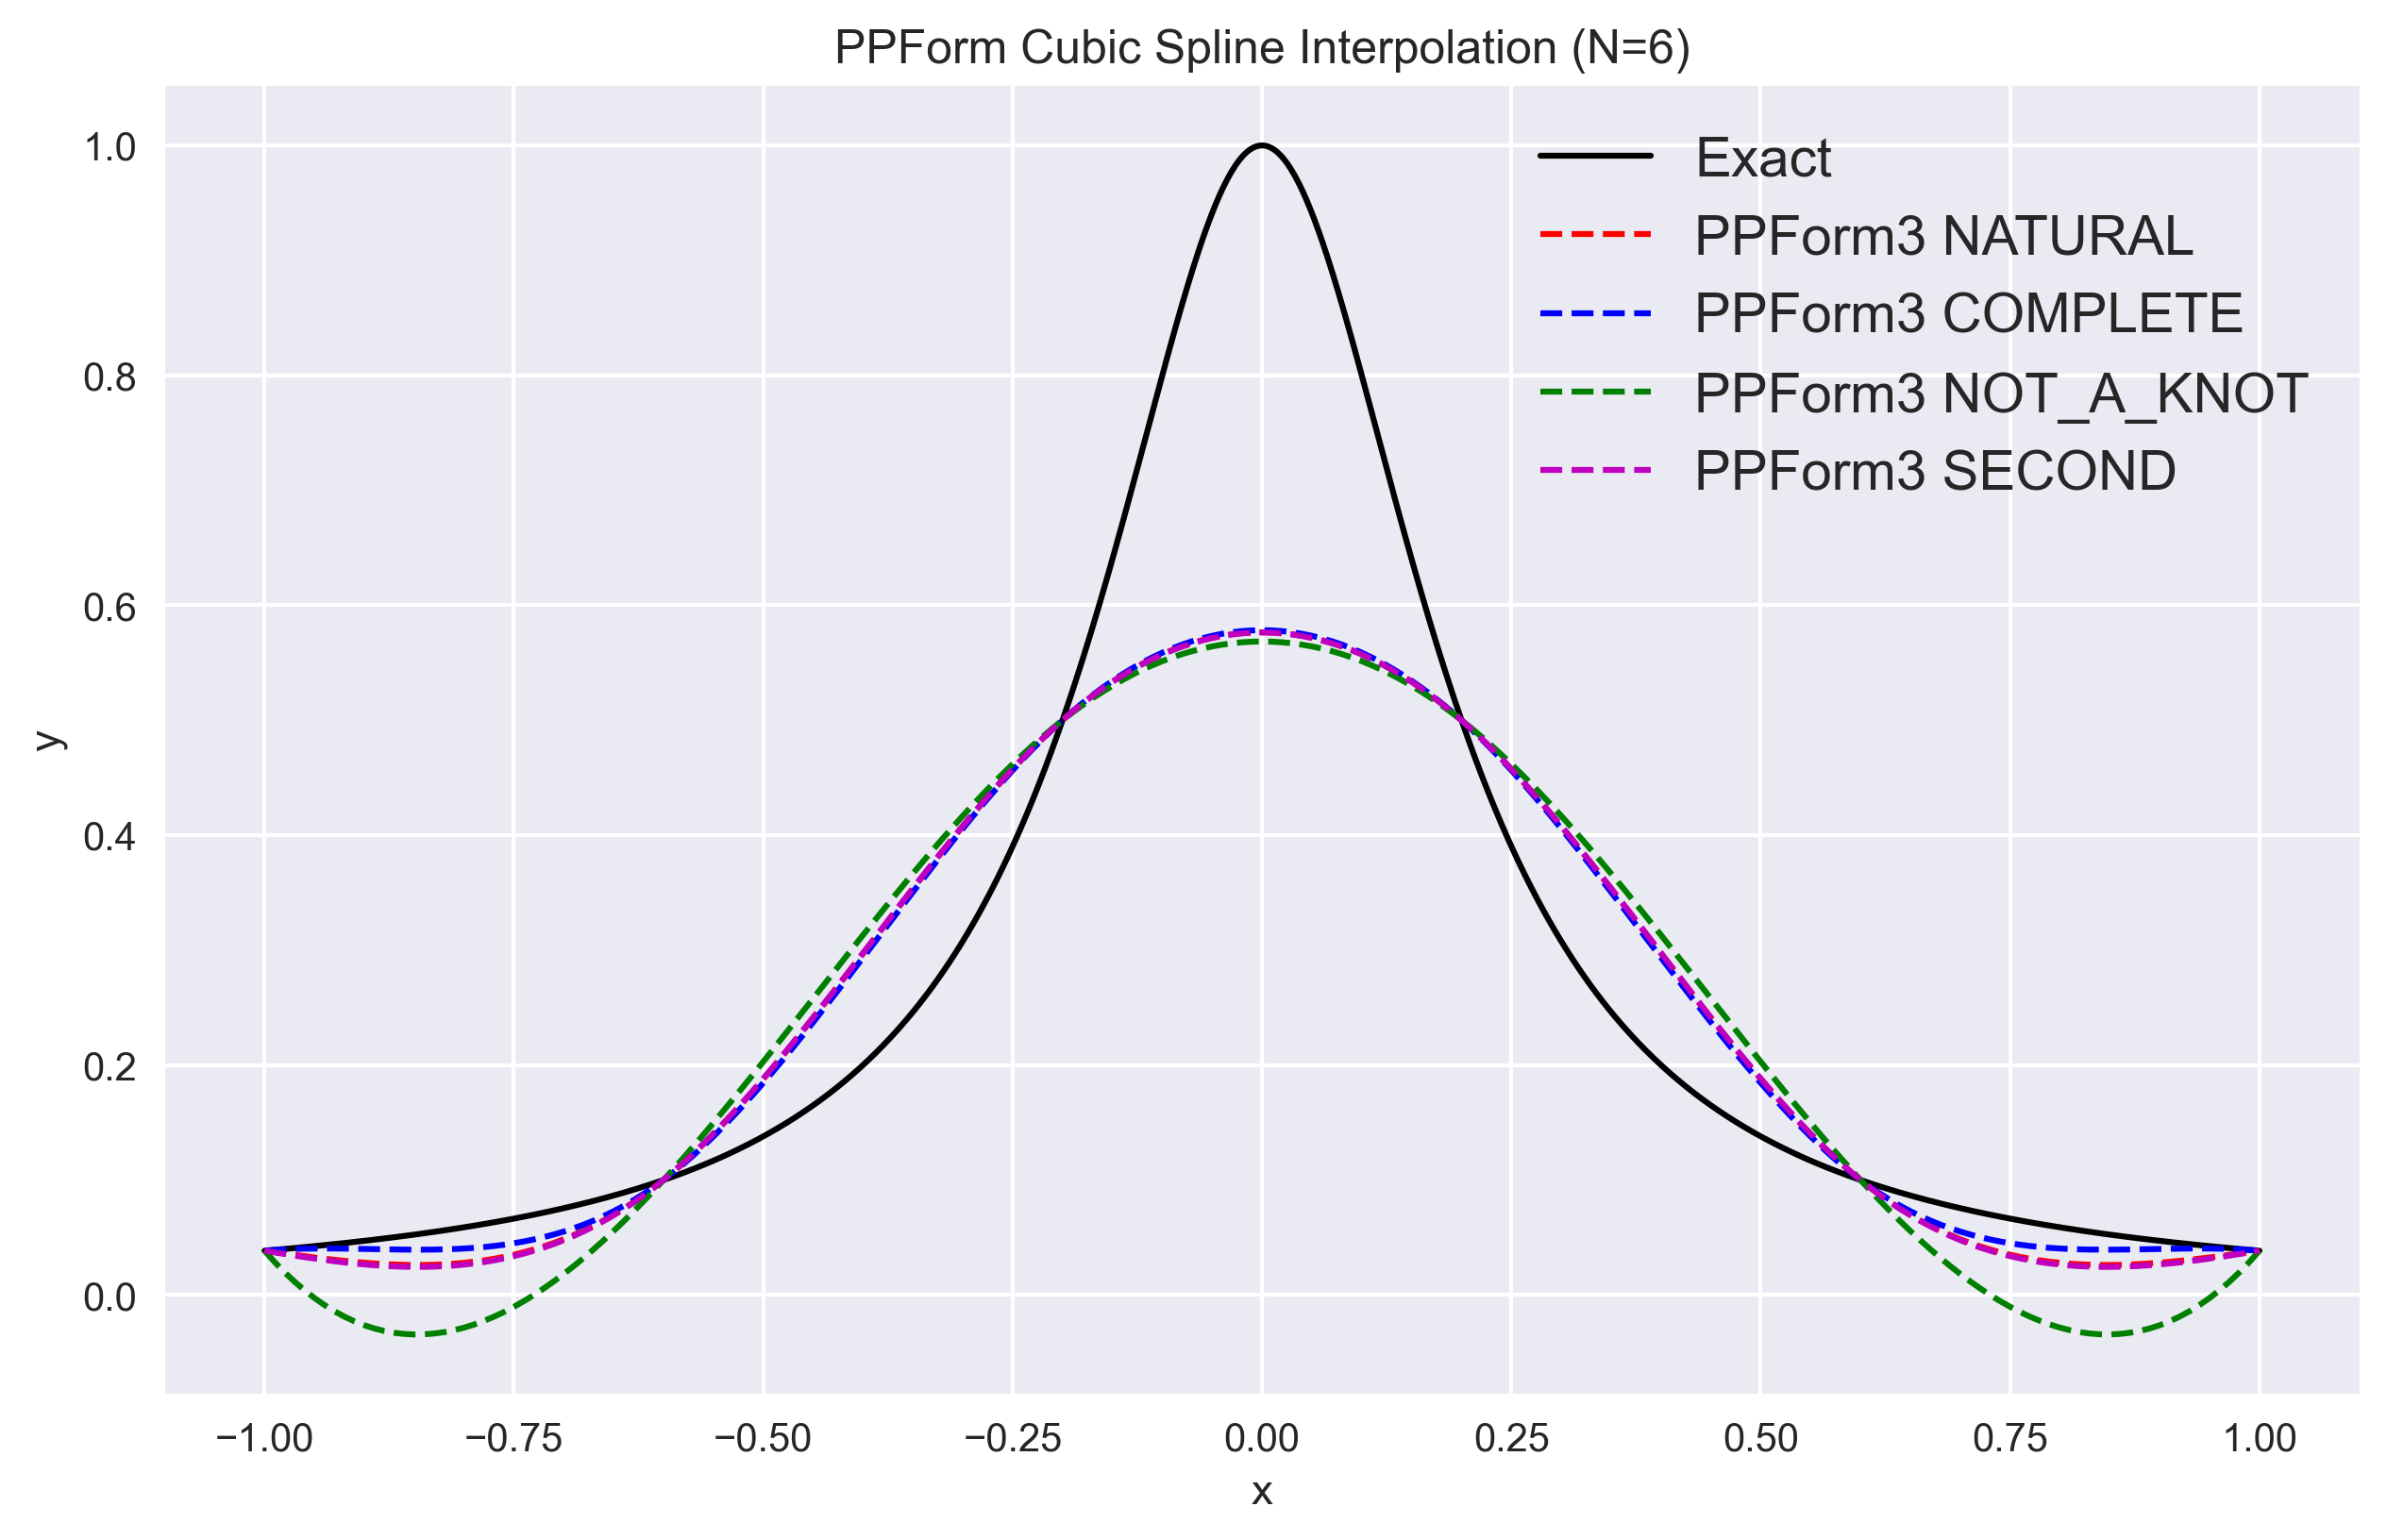
\includegraphics[width=0.45\textwidth]{../figure/problemA/PPForm3_N6.png}  &
    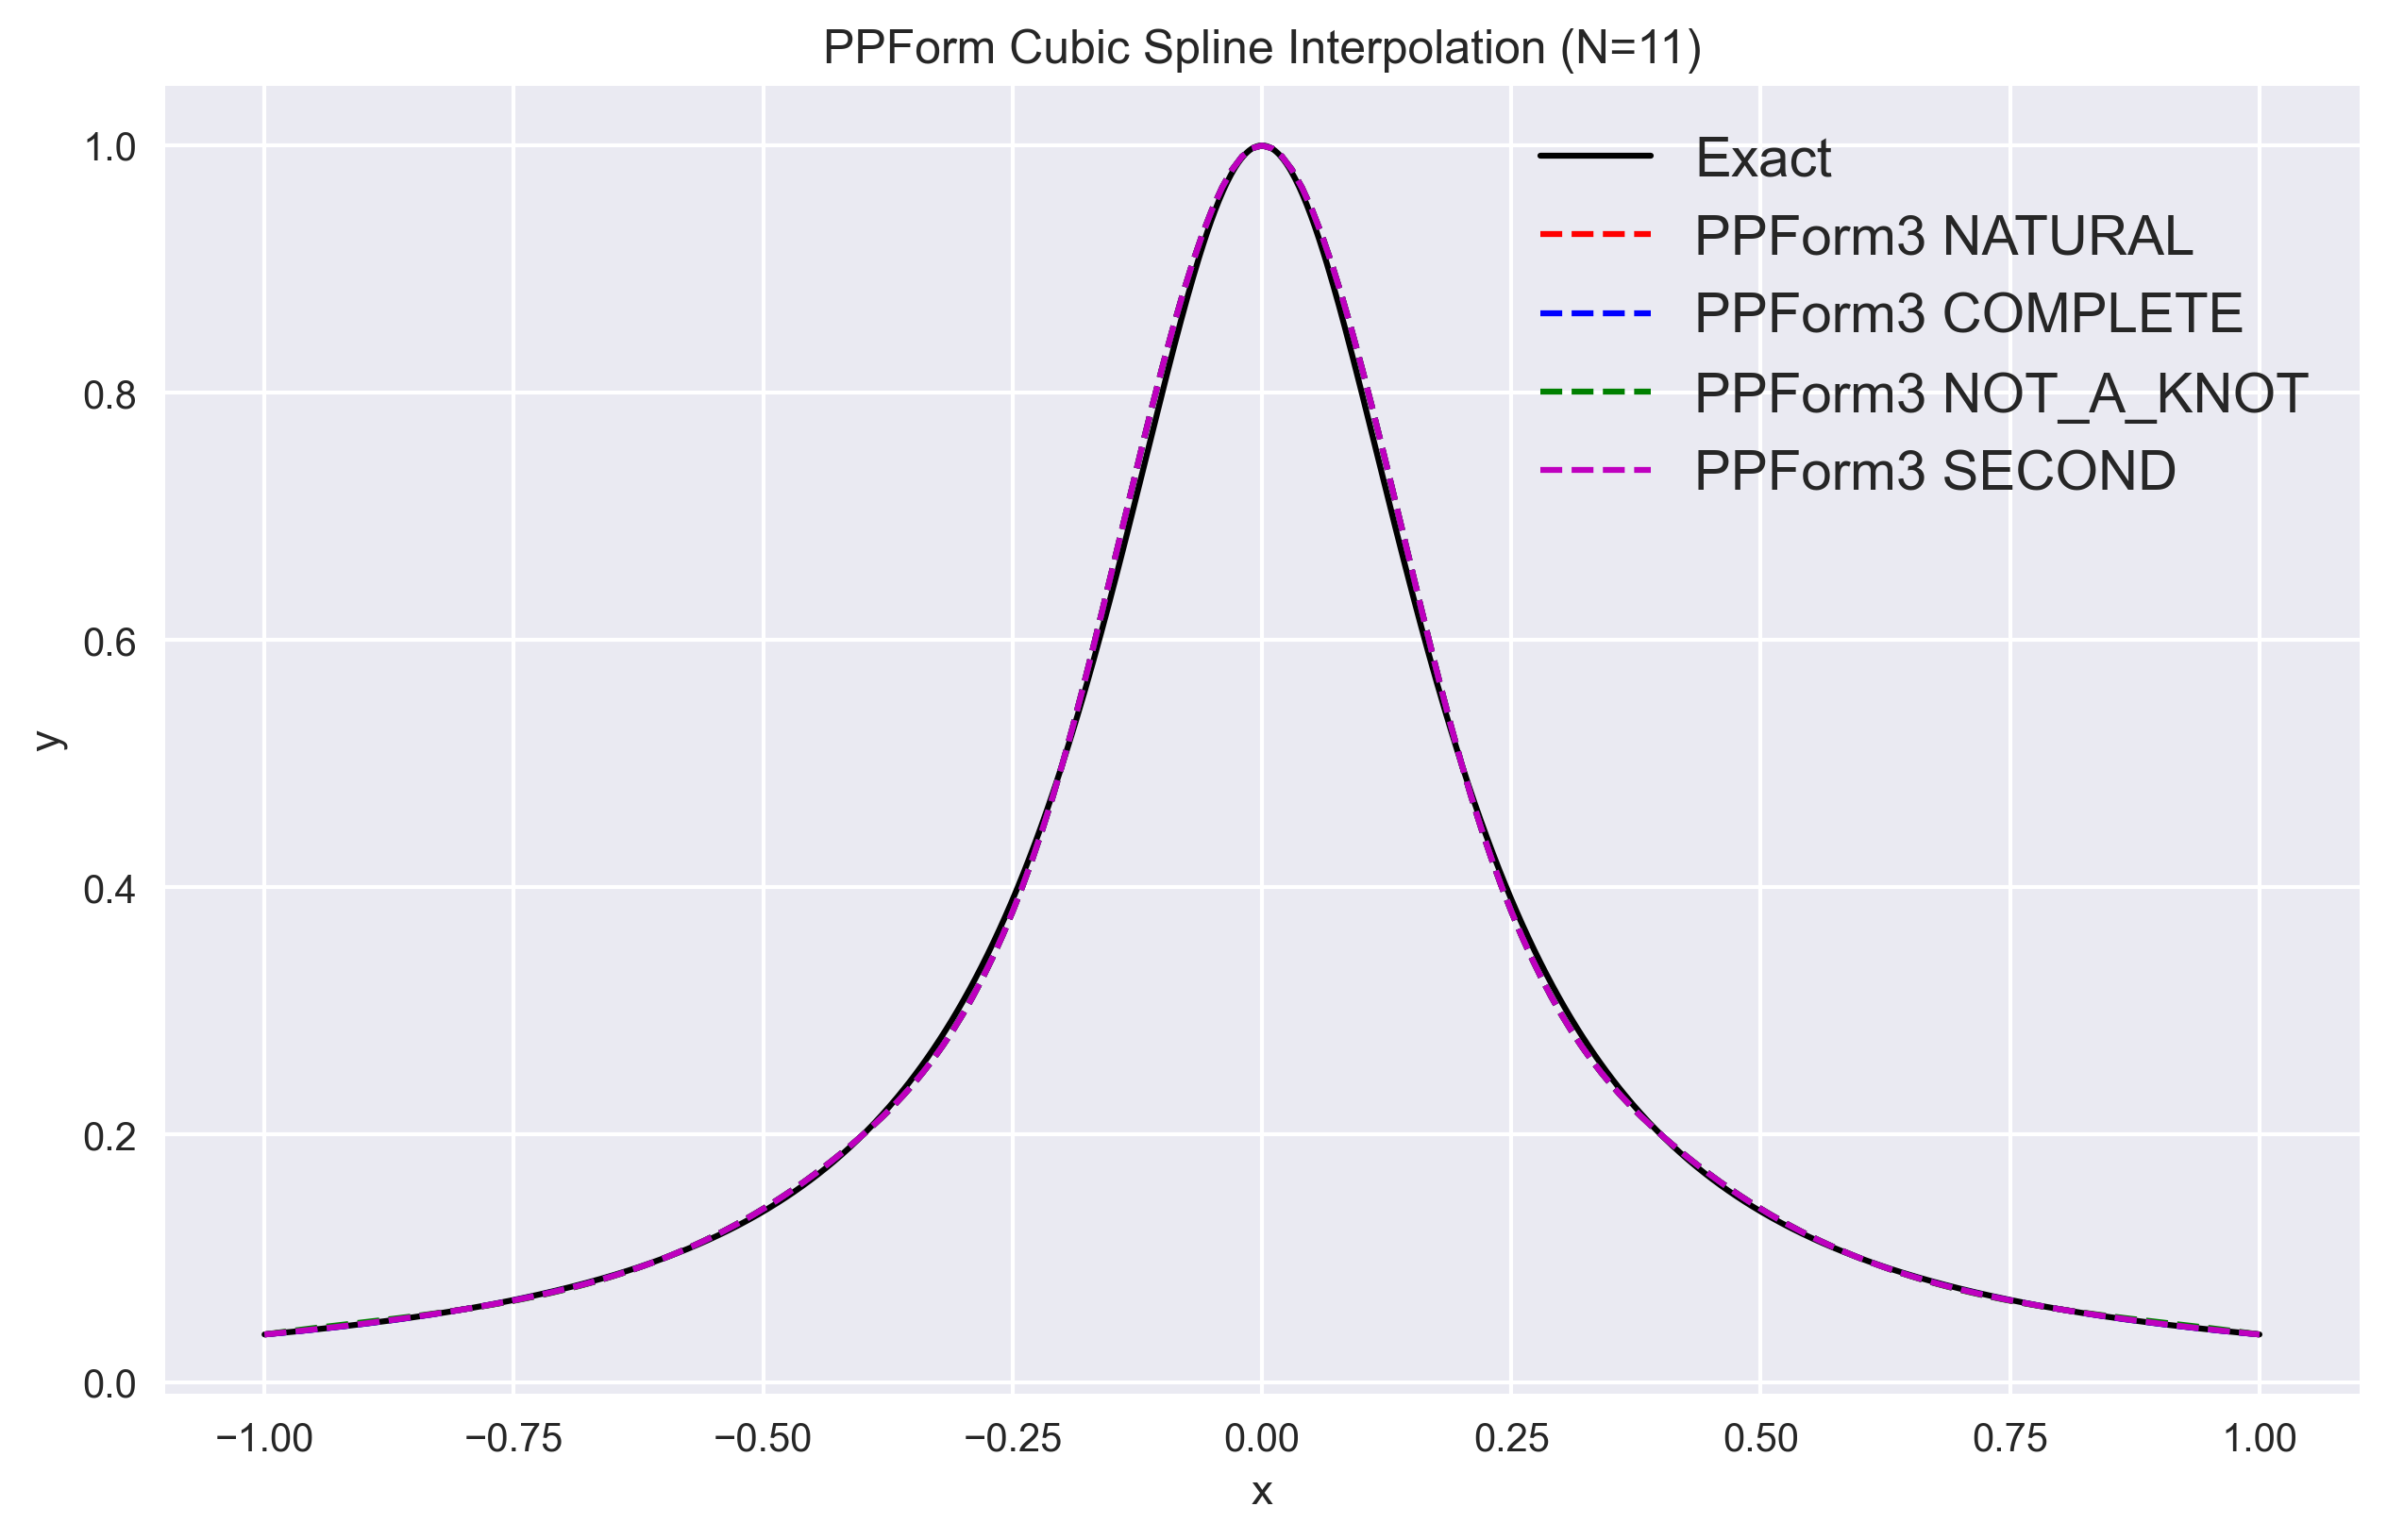
\includegraphics[width=0.45\textwidth]{../figure/problemA/PPForm3_N11.png}   \\
    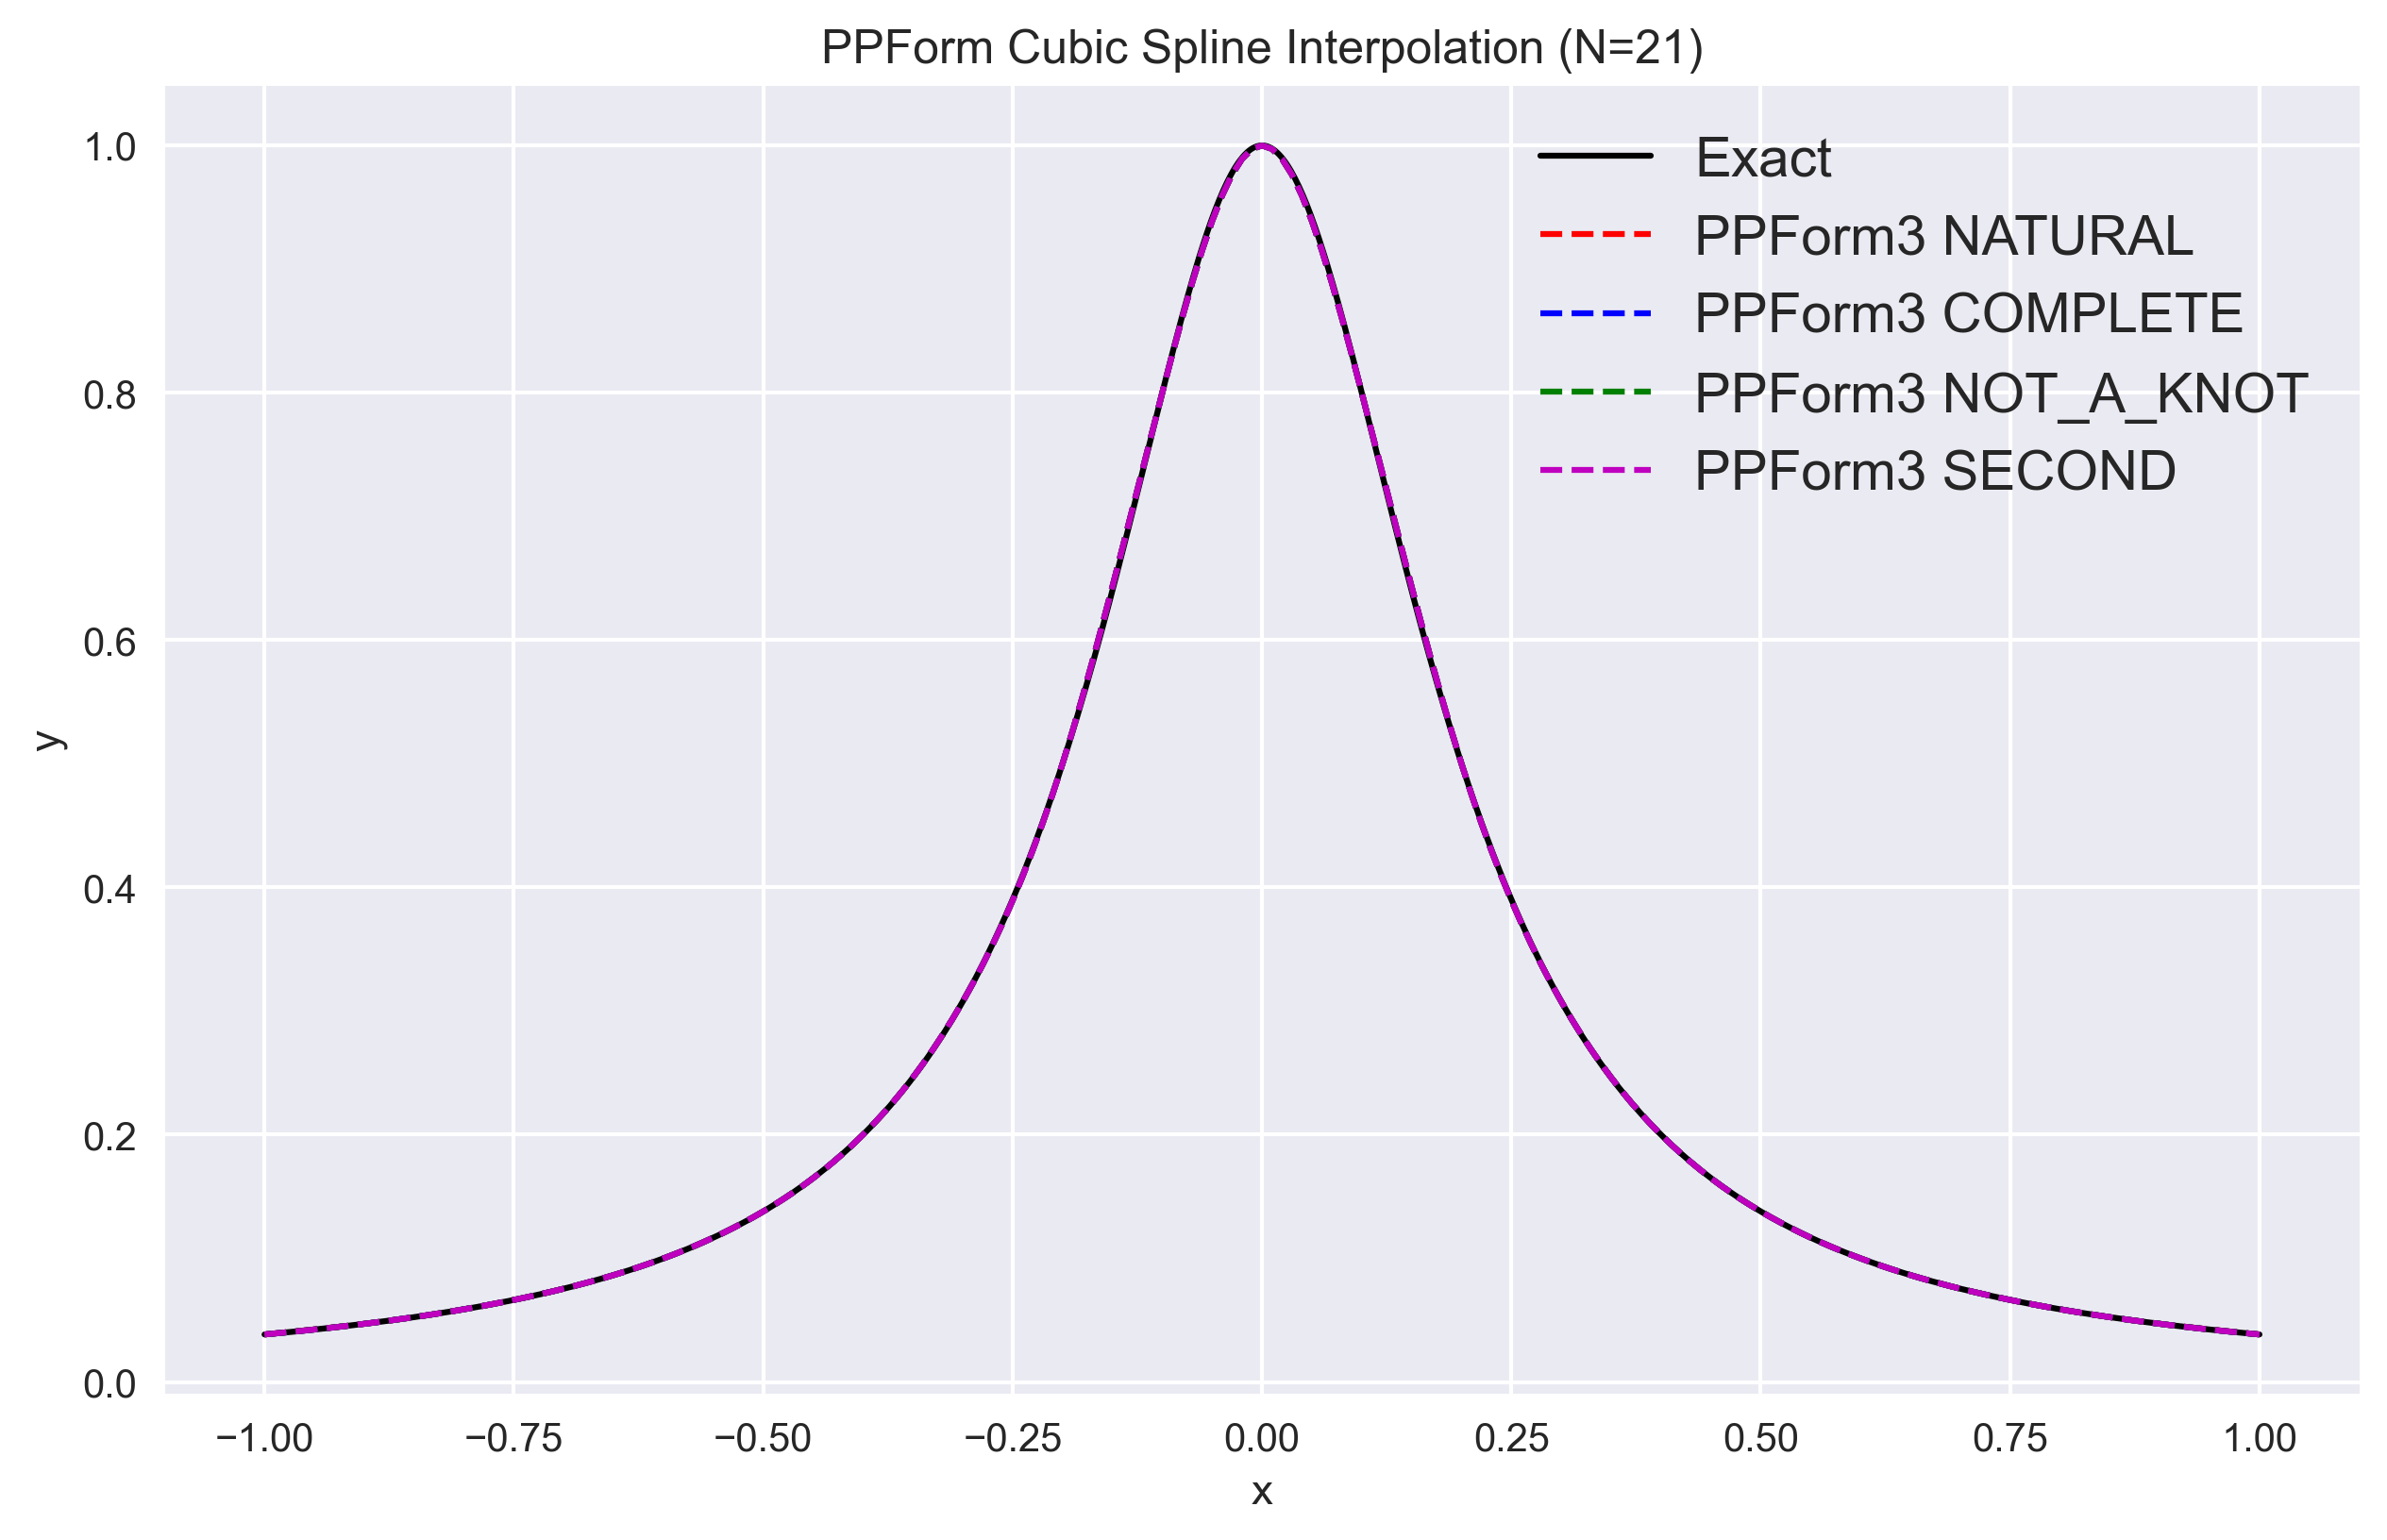
\includegraphics[width=0.45\textwidth]{../figure/problemA/PPForm3_N21.png} &
    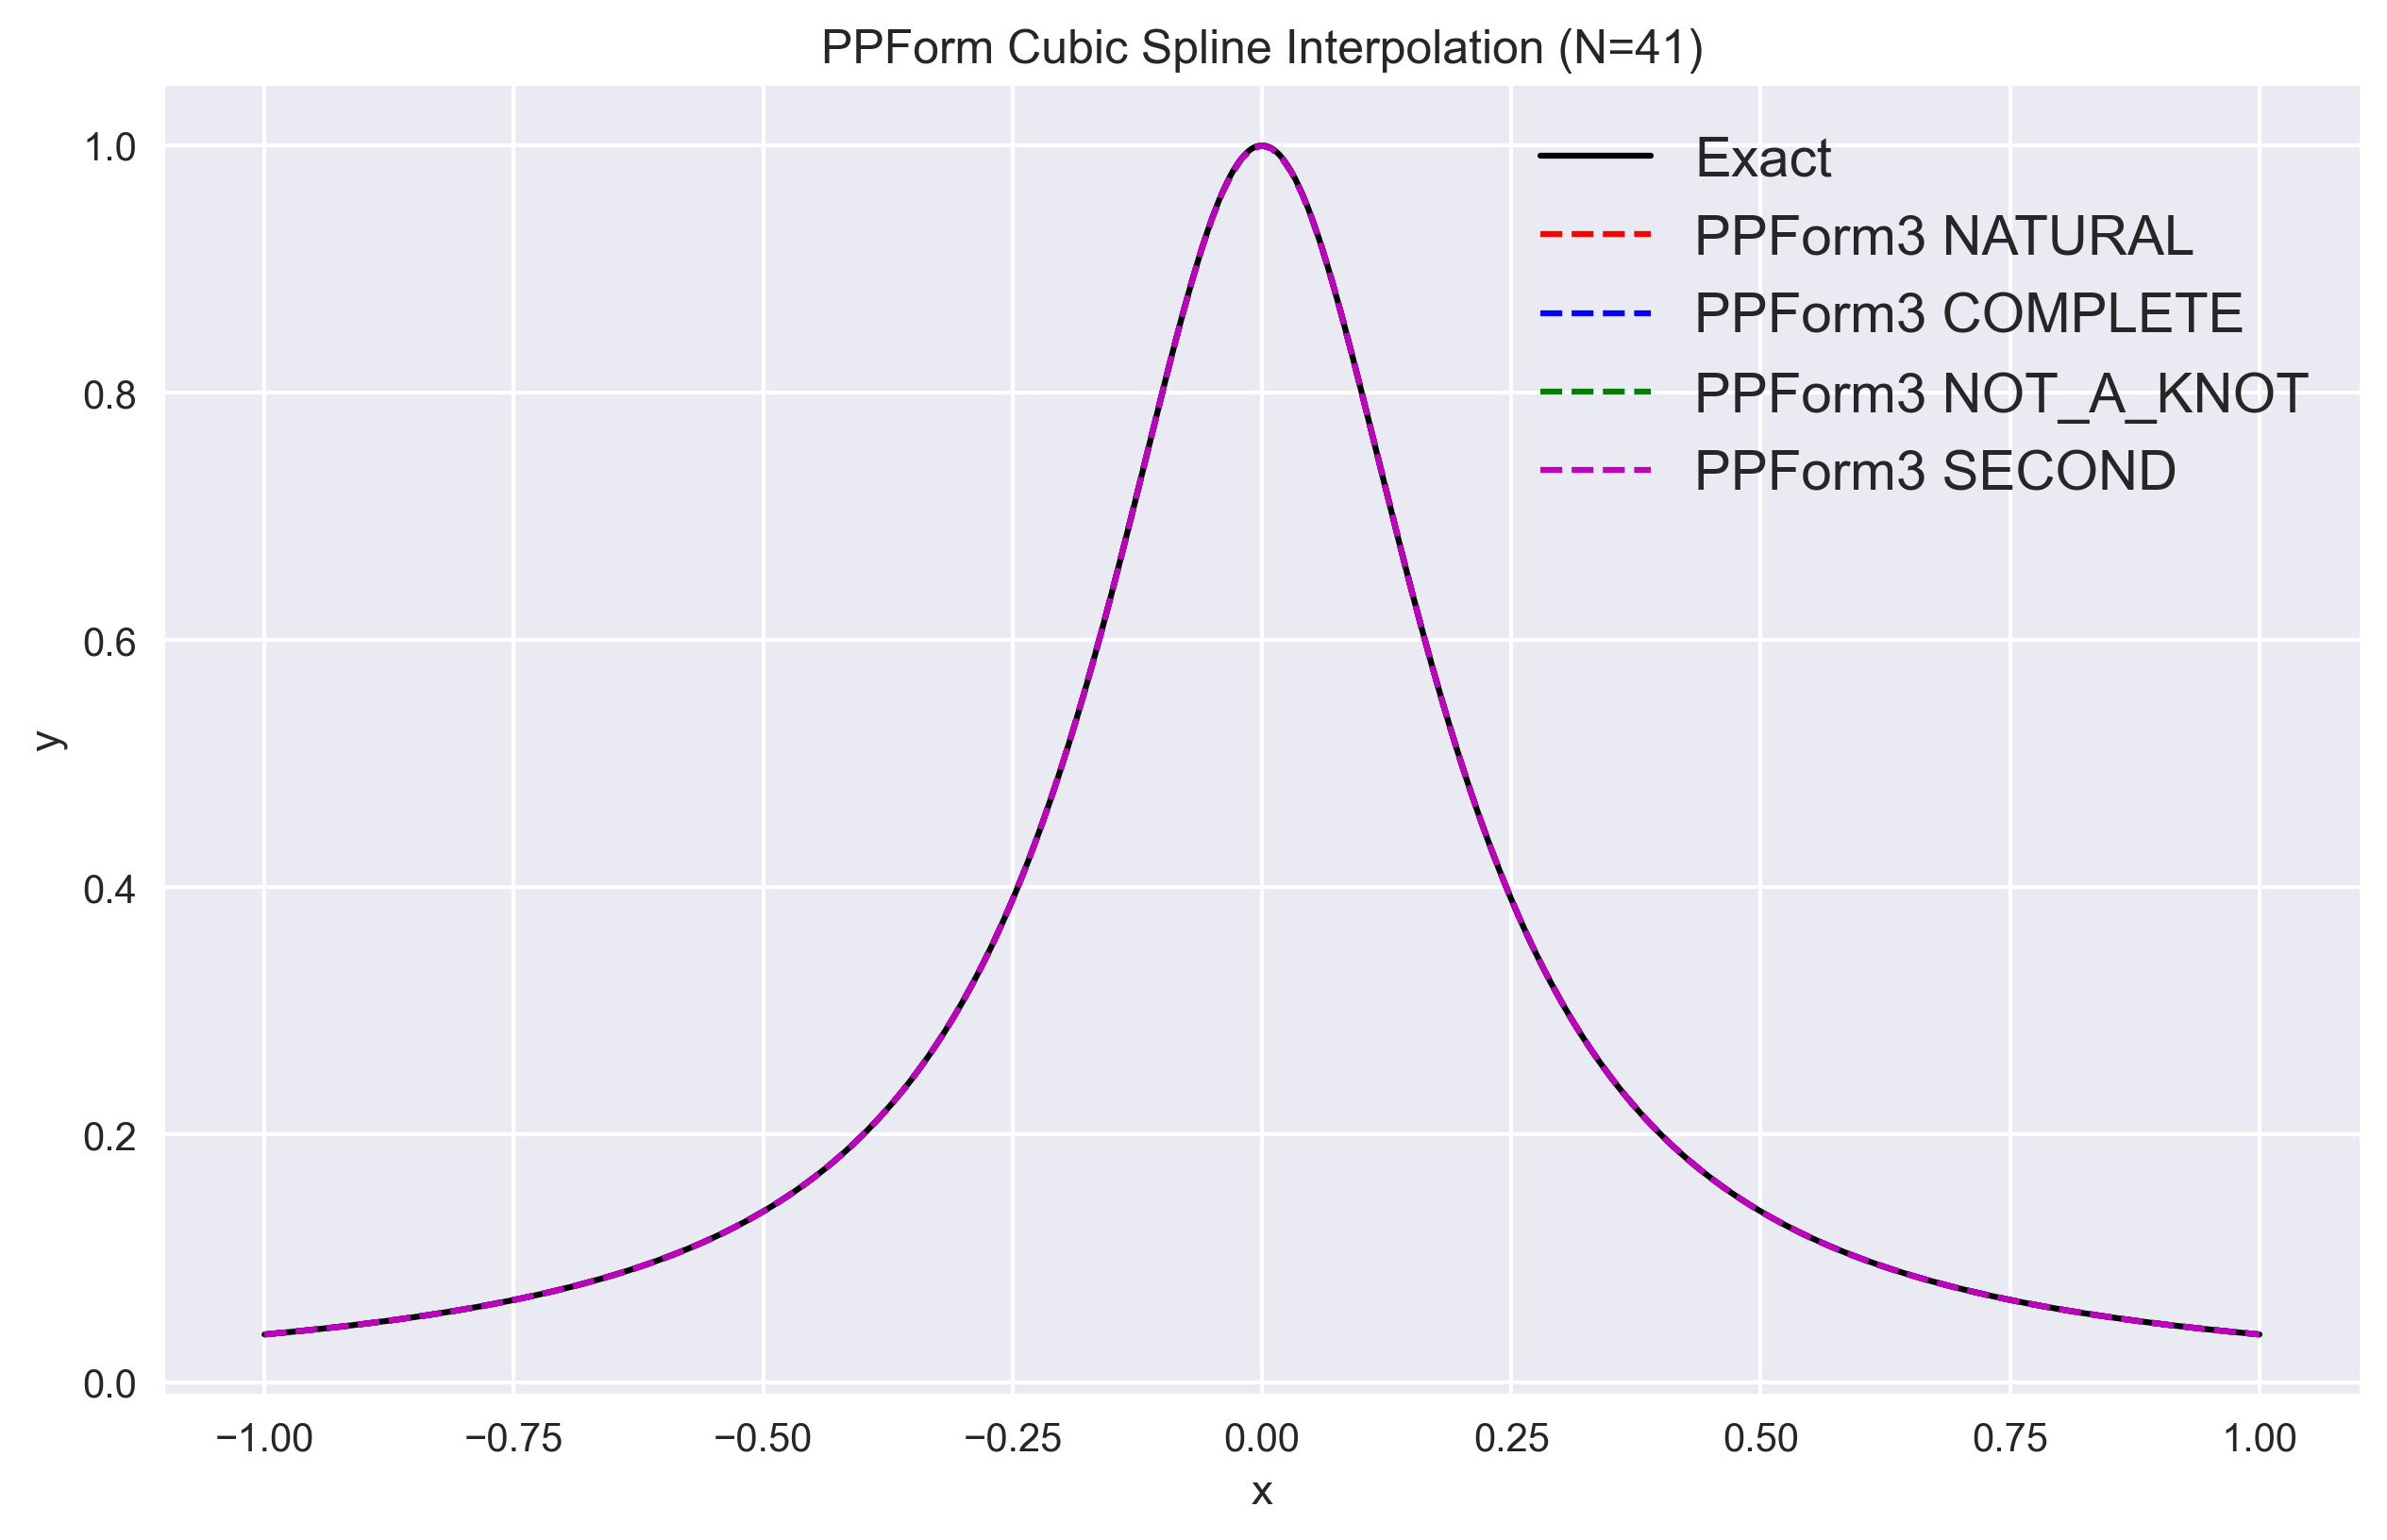
\includegraphics[width=0.45\textwidth]{../figure/problemA/PPForm3_N41.png}   \\
    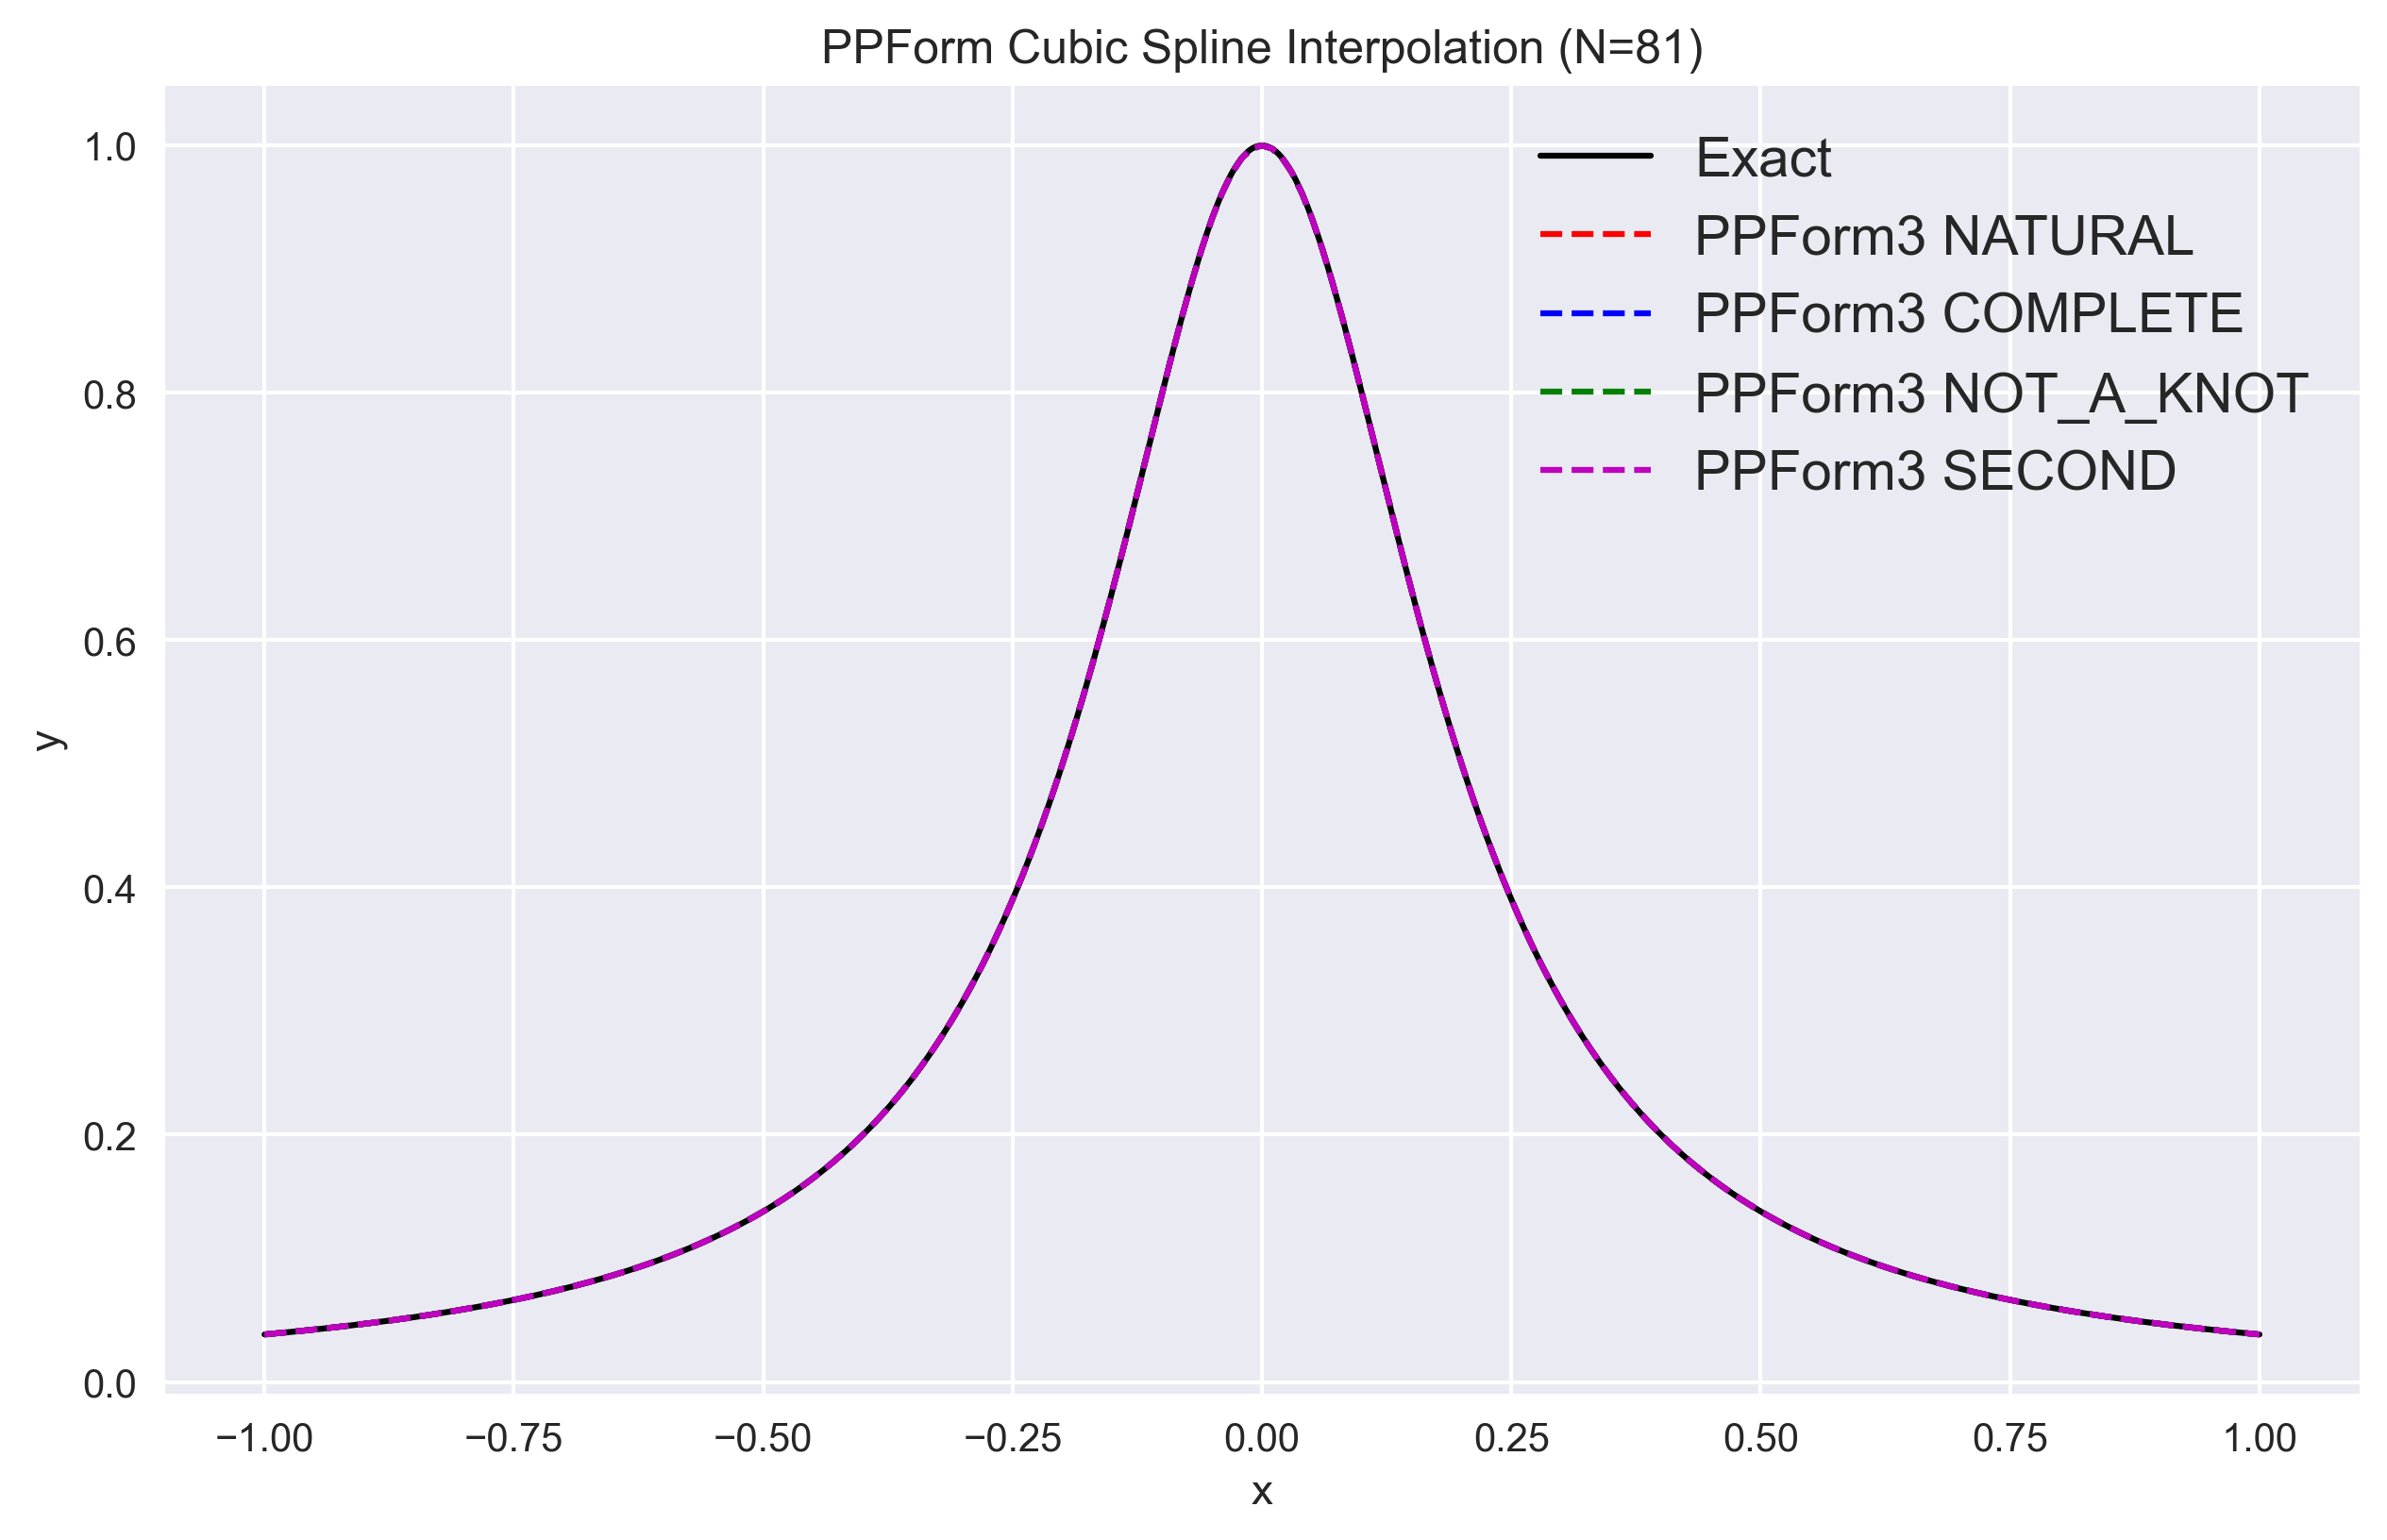
\includegraphics[width=0.45\textwidth]{../figure/problemA/PPForm3_N81.png} &
  \end{tabular}
  \renewcommand{\figurename}{Fig.}
  \caption{Interpolation curves for different boundary conditions by cubic PPForm splines}
  \label{fig:A_ppform3}
\end{figure}

As shown in Fig.\ref{fig:A_linear}, the interpolation curves for linear PPForm
and BSpline splines with different numbers of uniform interpolation points are
displayed.

In fact, from the output interpolation data, it can be seen that both produce
the same curves when using the same interpolation points and boundary
conditions for linear interpolation.

\begin{figure}[H]
  \centering
  \begin{tabular}{cc}
    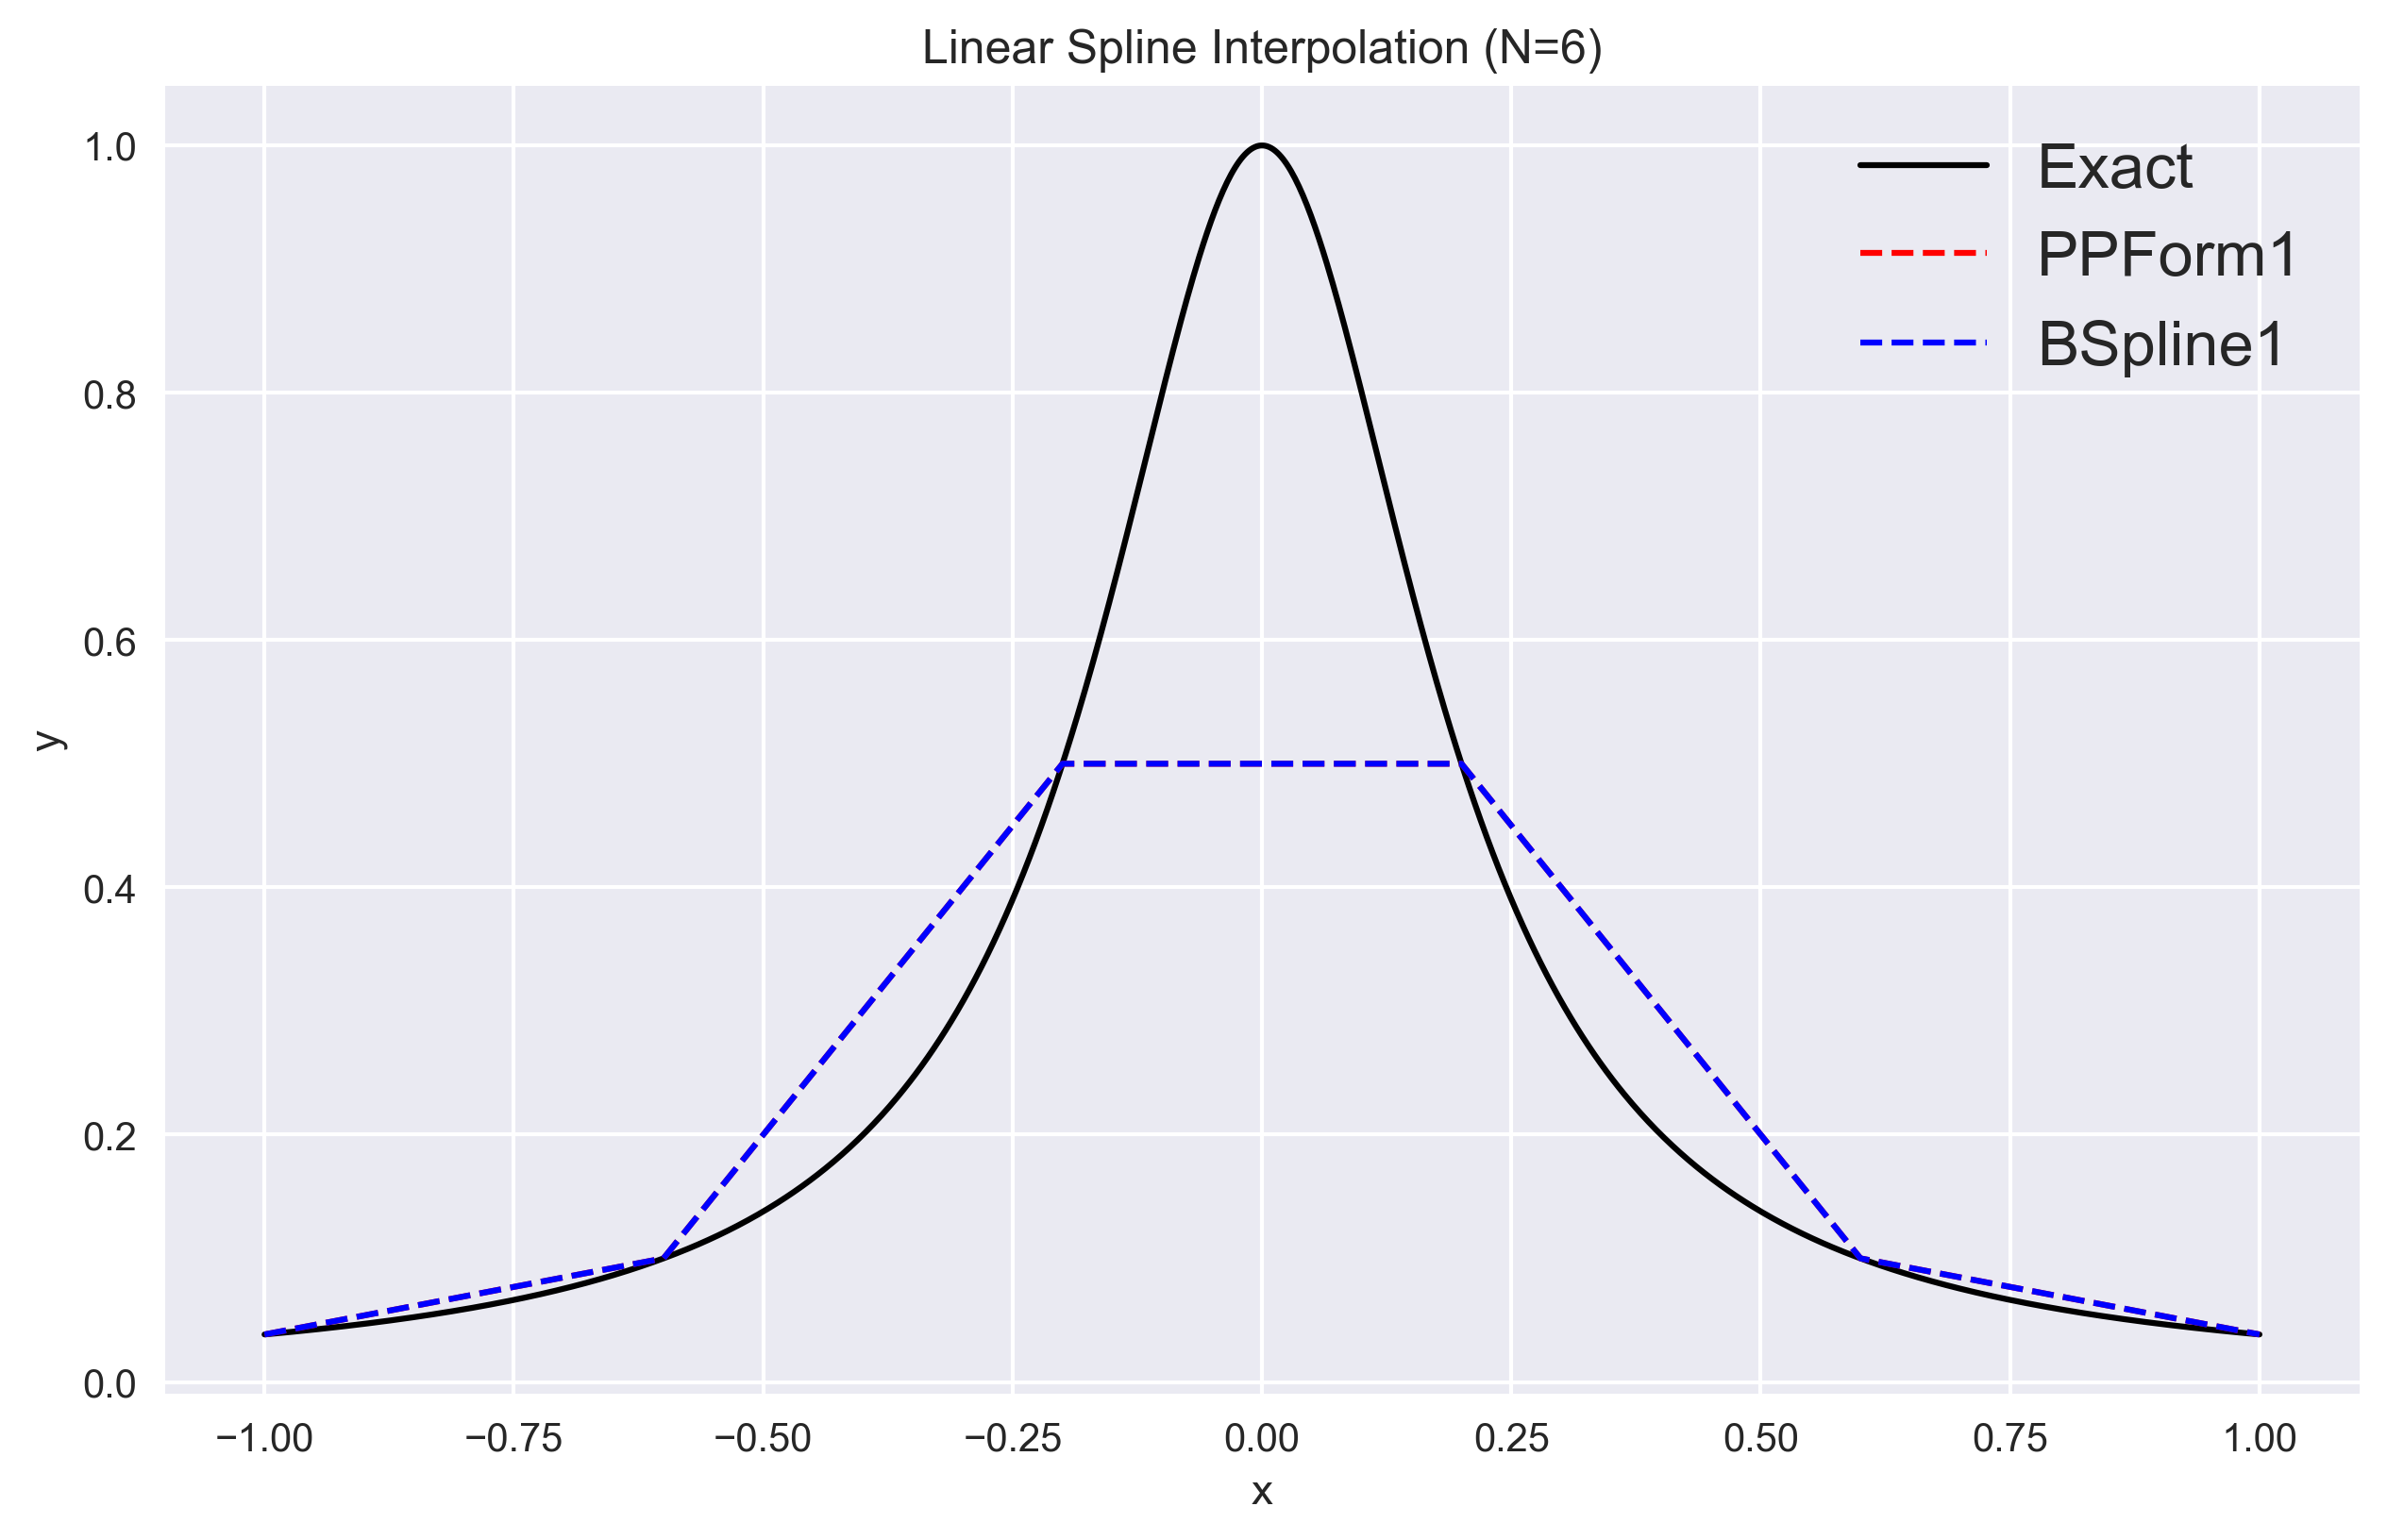
\includegraphics[width=0.45\textwidth]{../figure/problemA/linear_N6.png}  &
    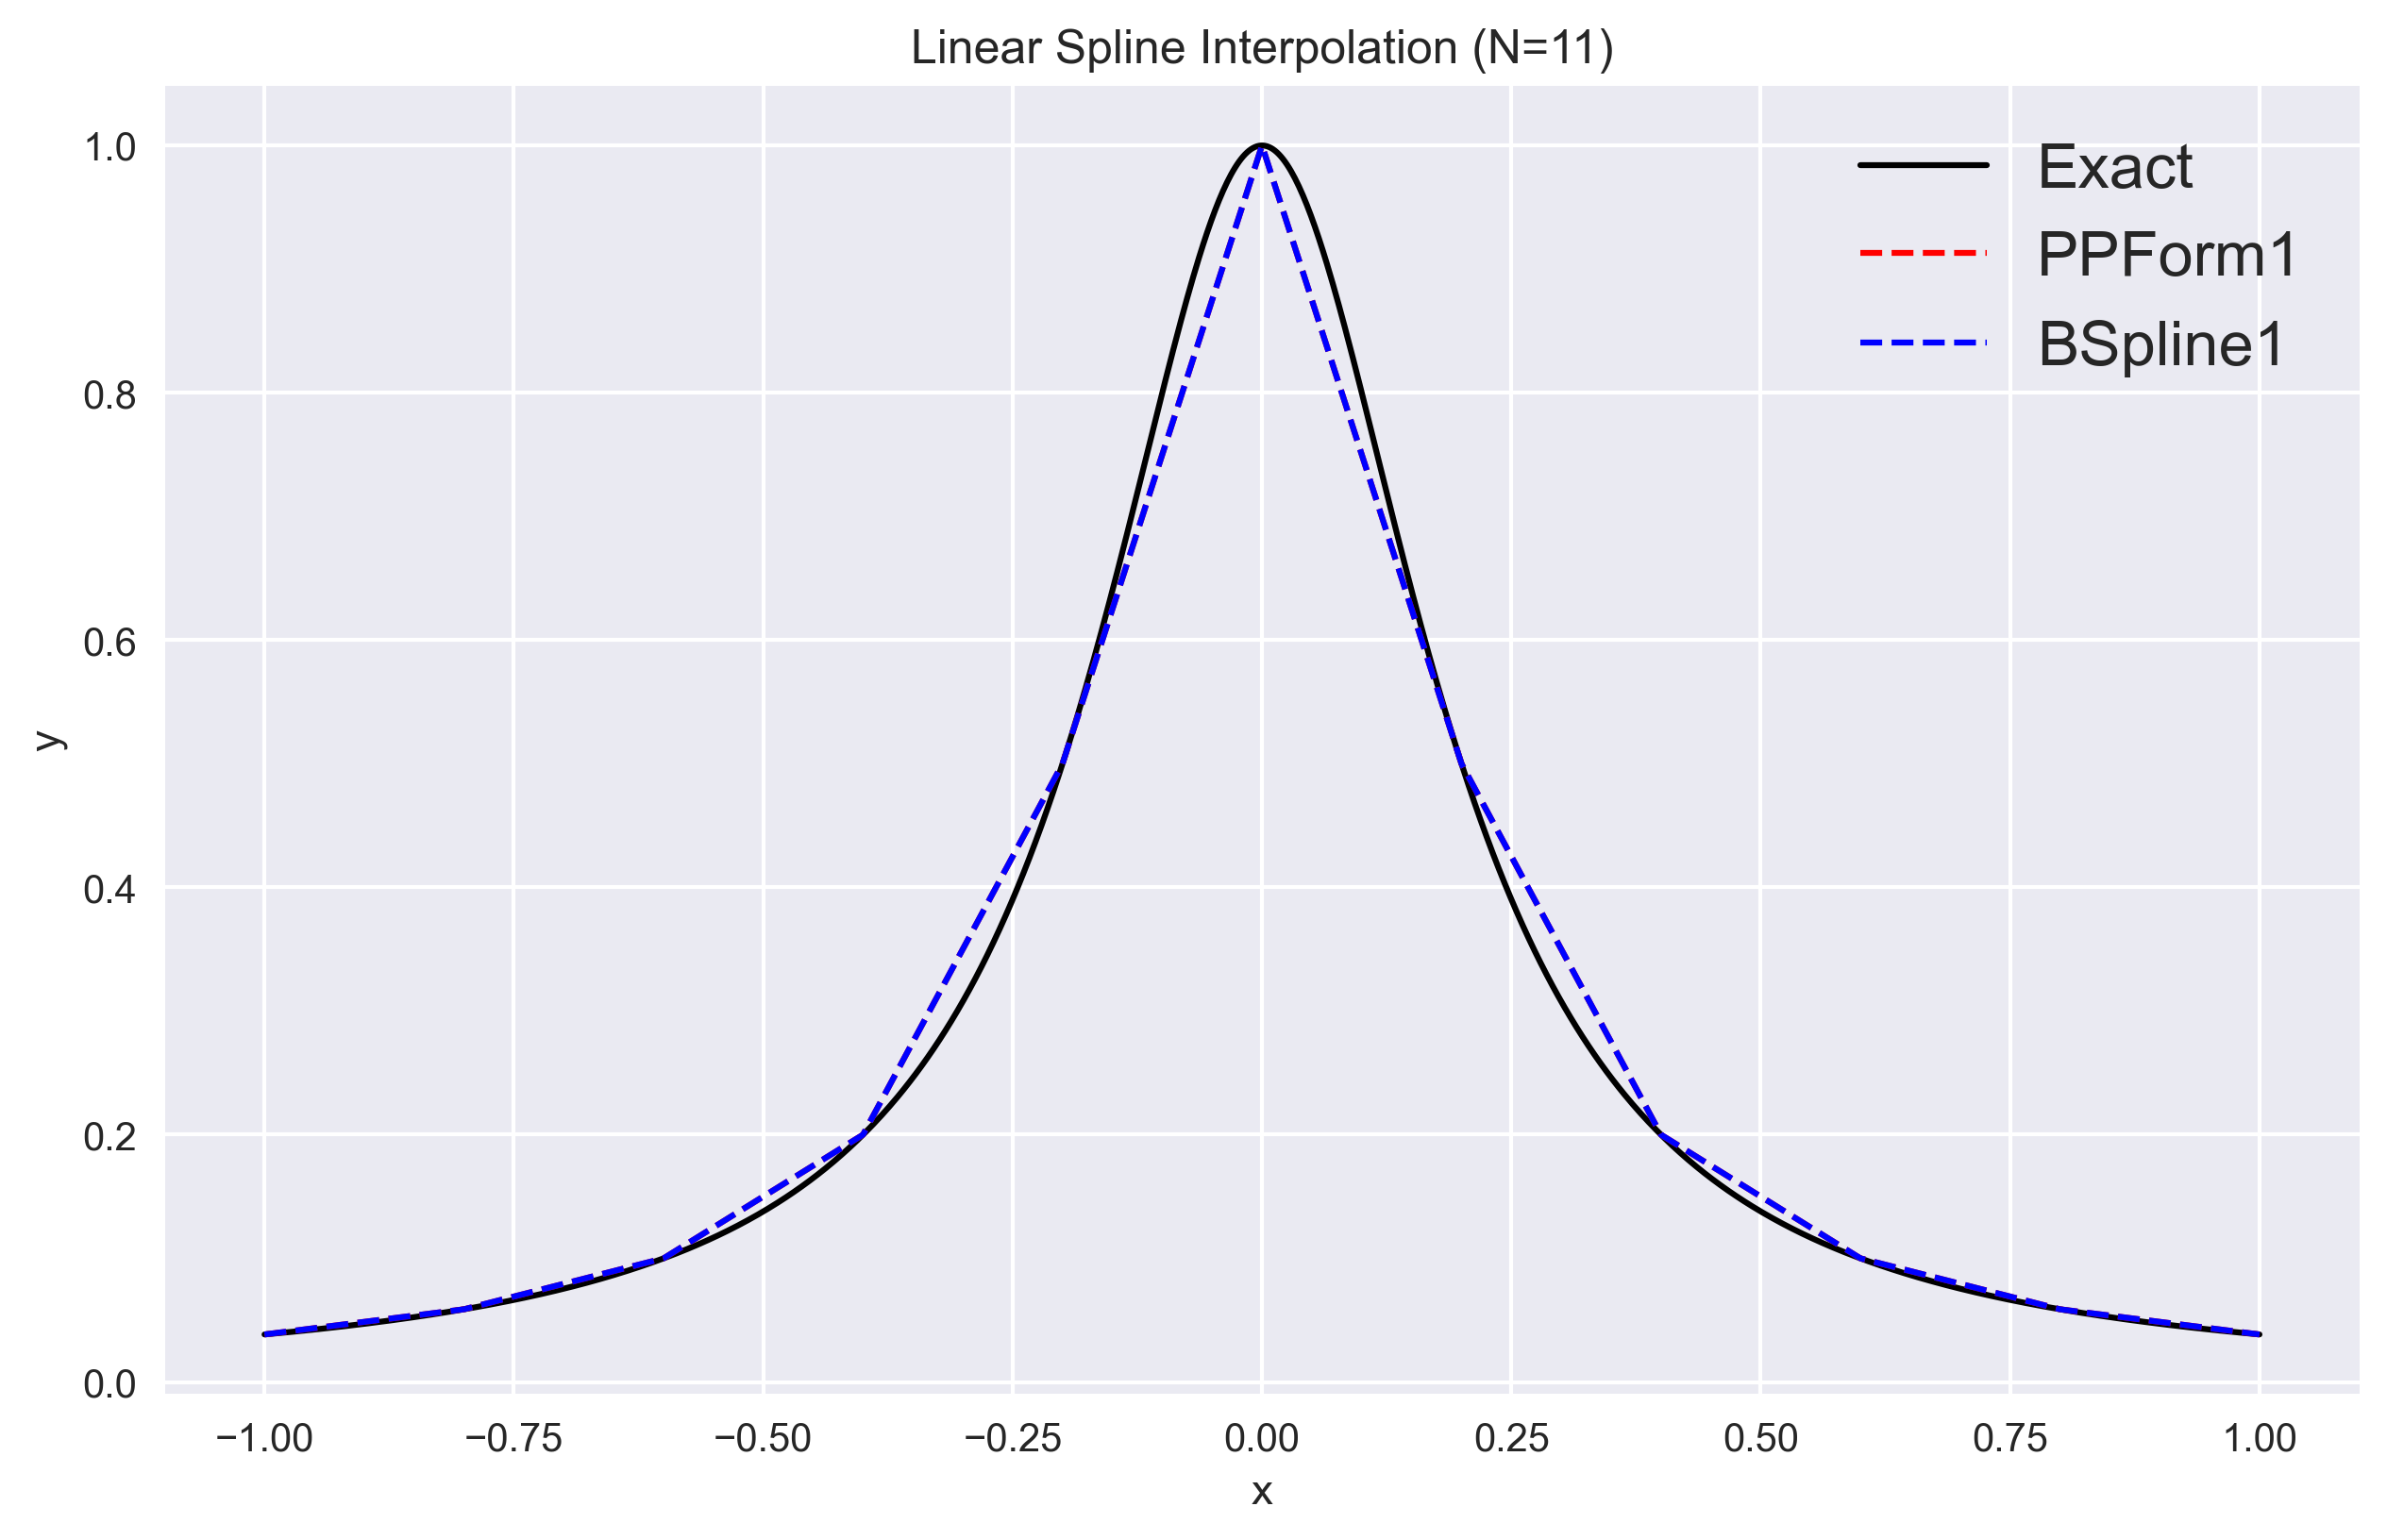
\includegraphics[width=0.45\textwidth]{../figure/problemA/linear_N11.png}   \\
    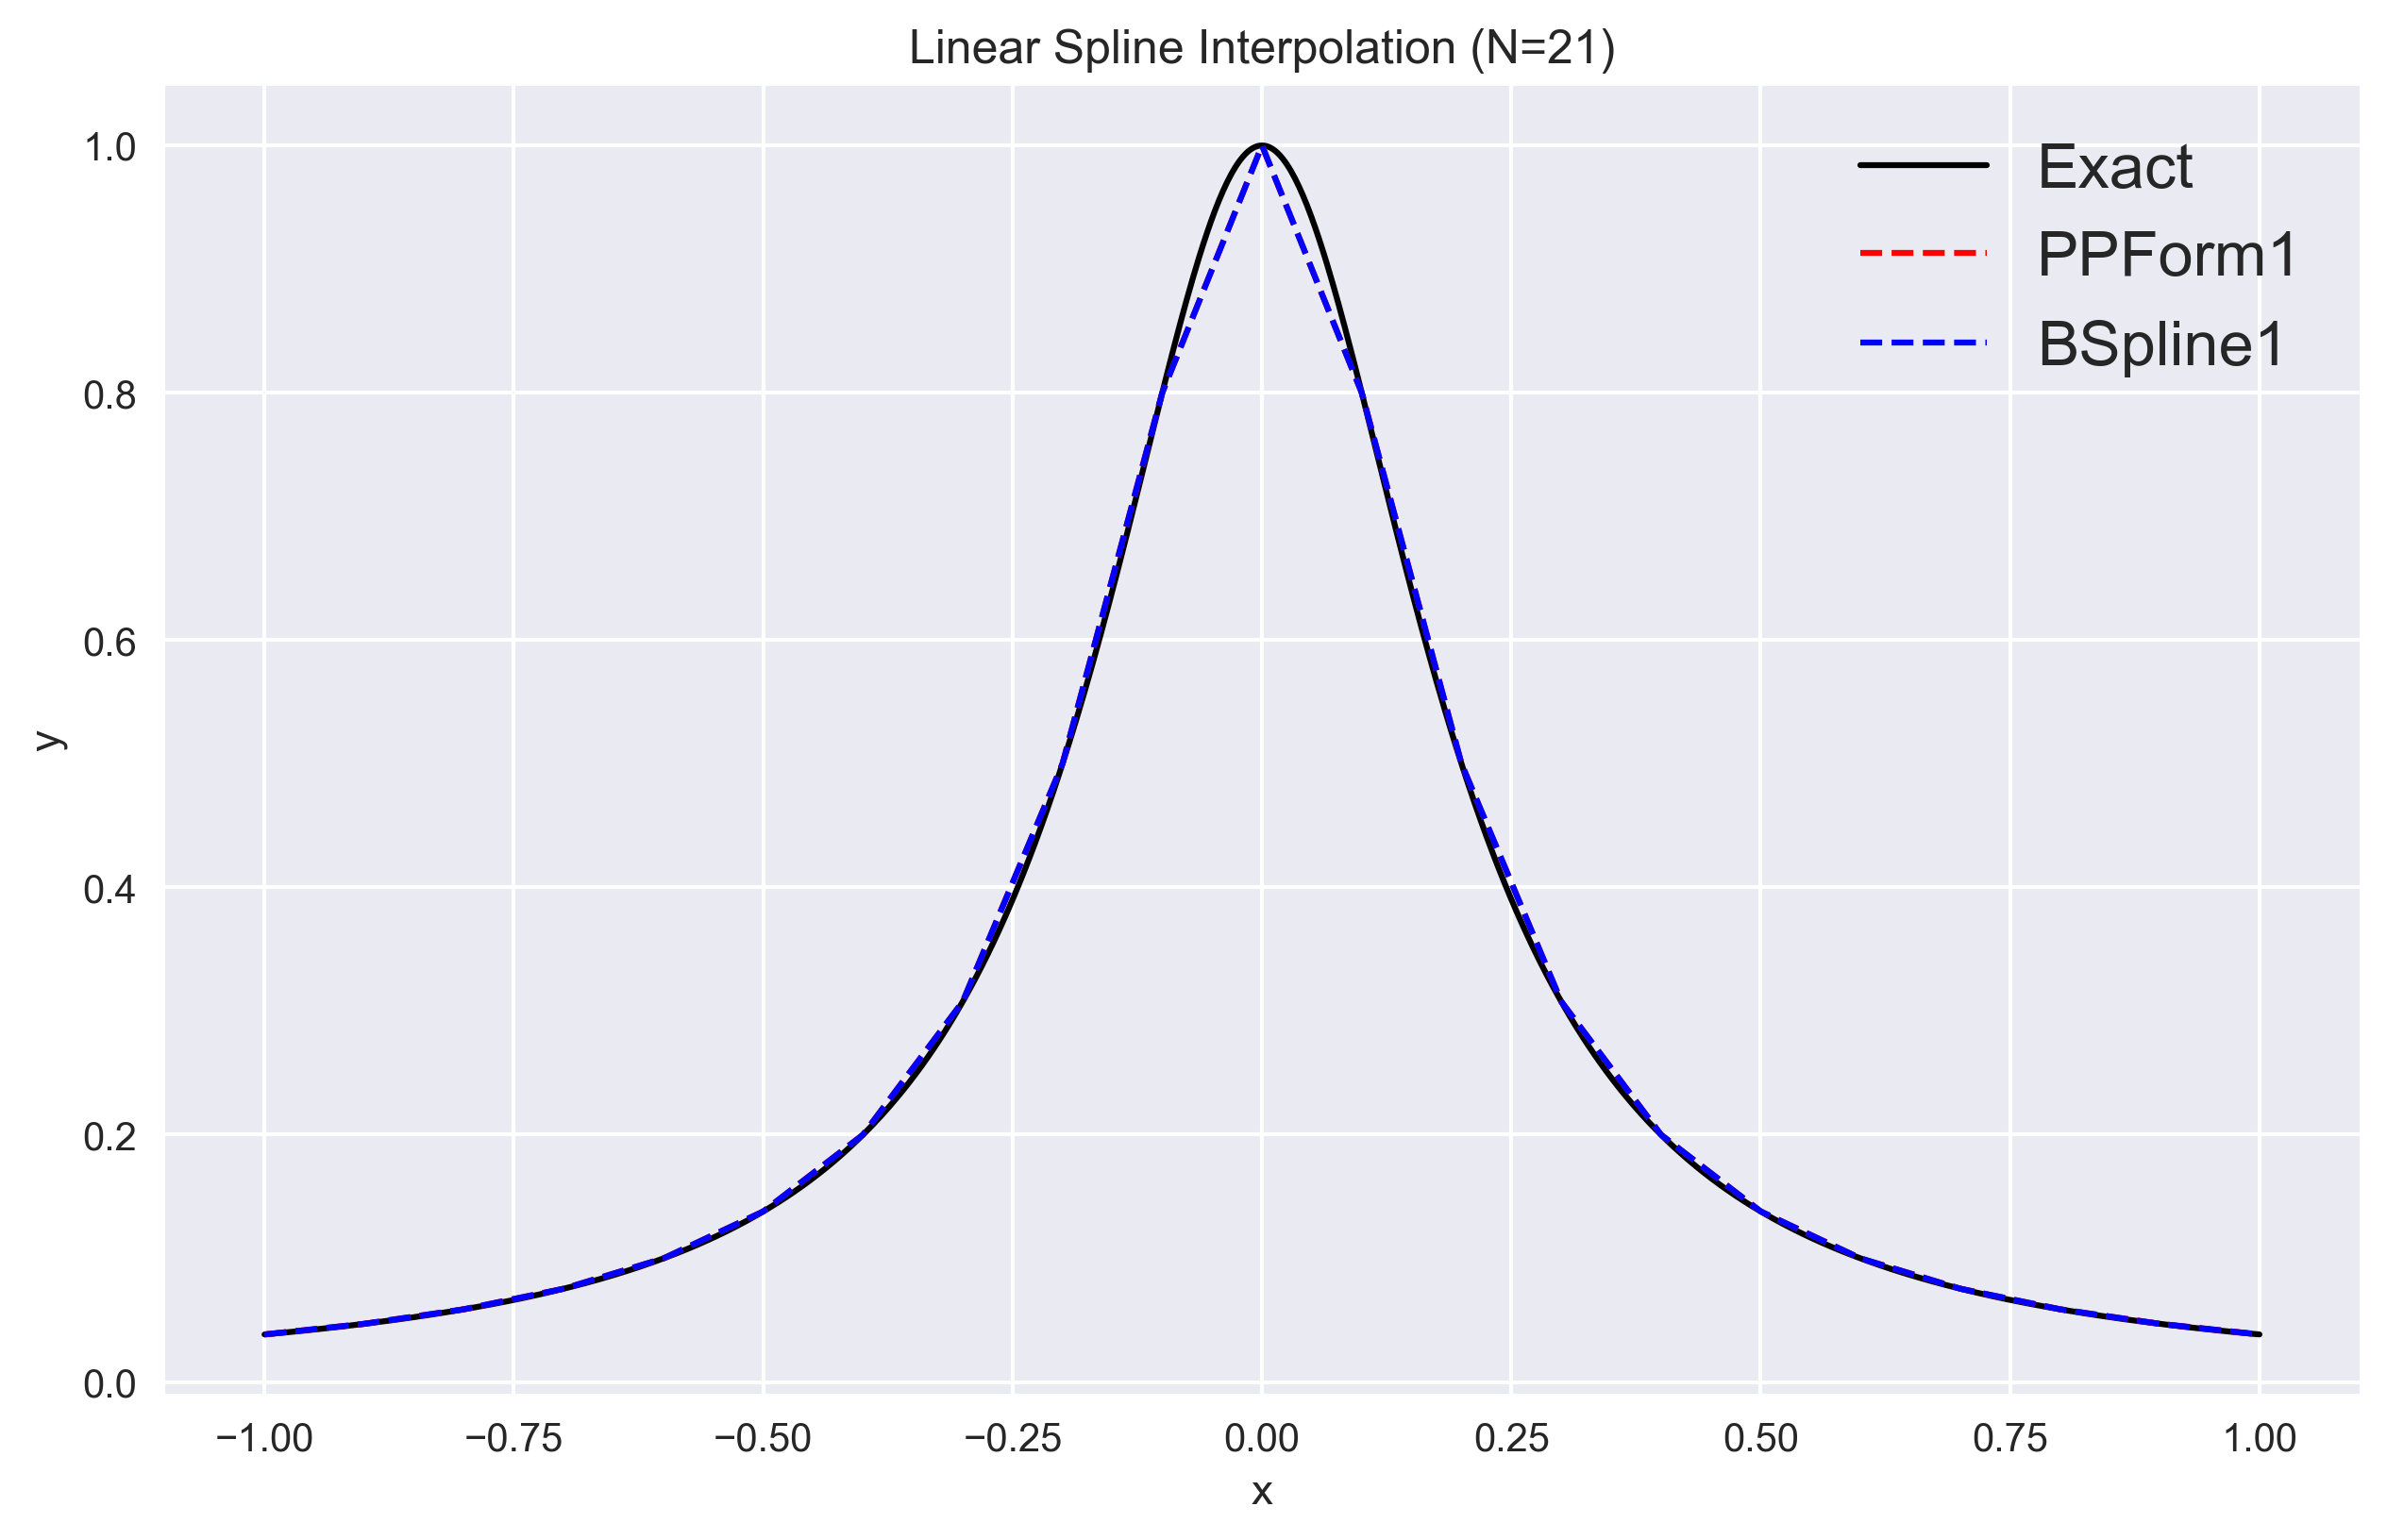
\includegraphics[width=0.45\textwidth]{../figure/problemA/linear_N21.png} &
    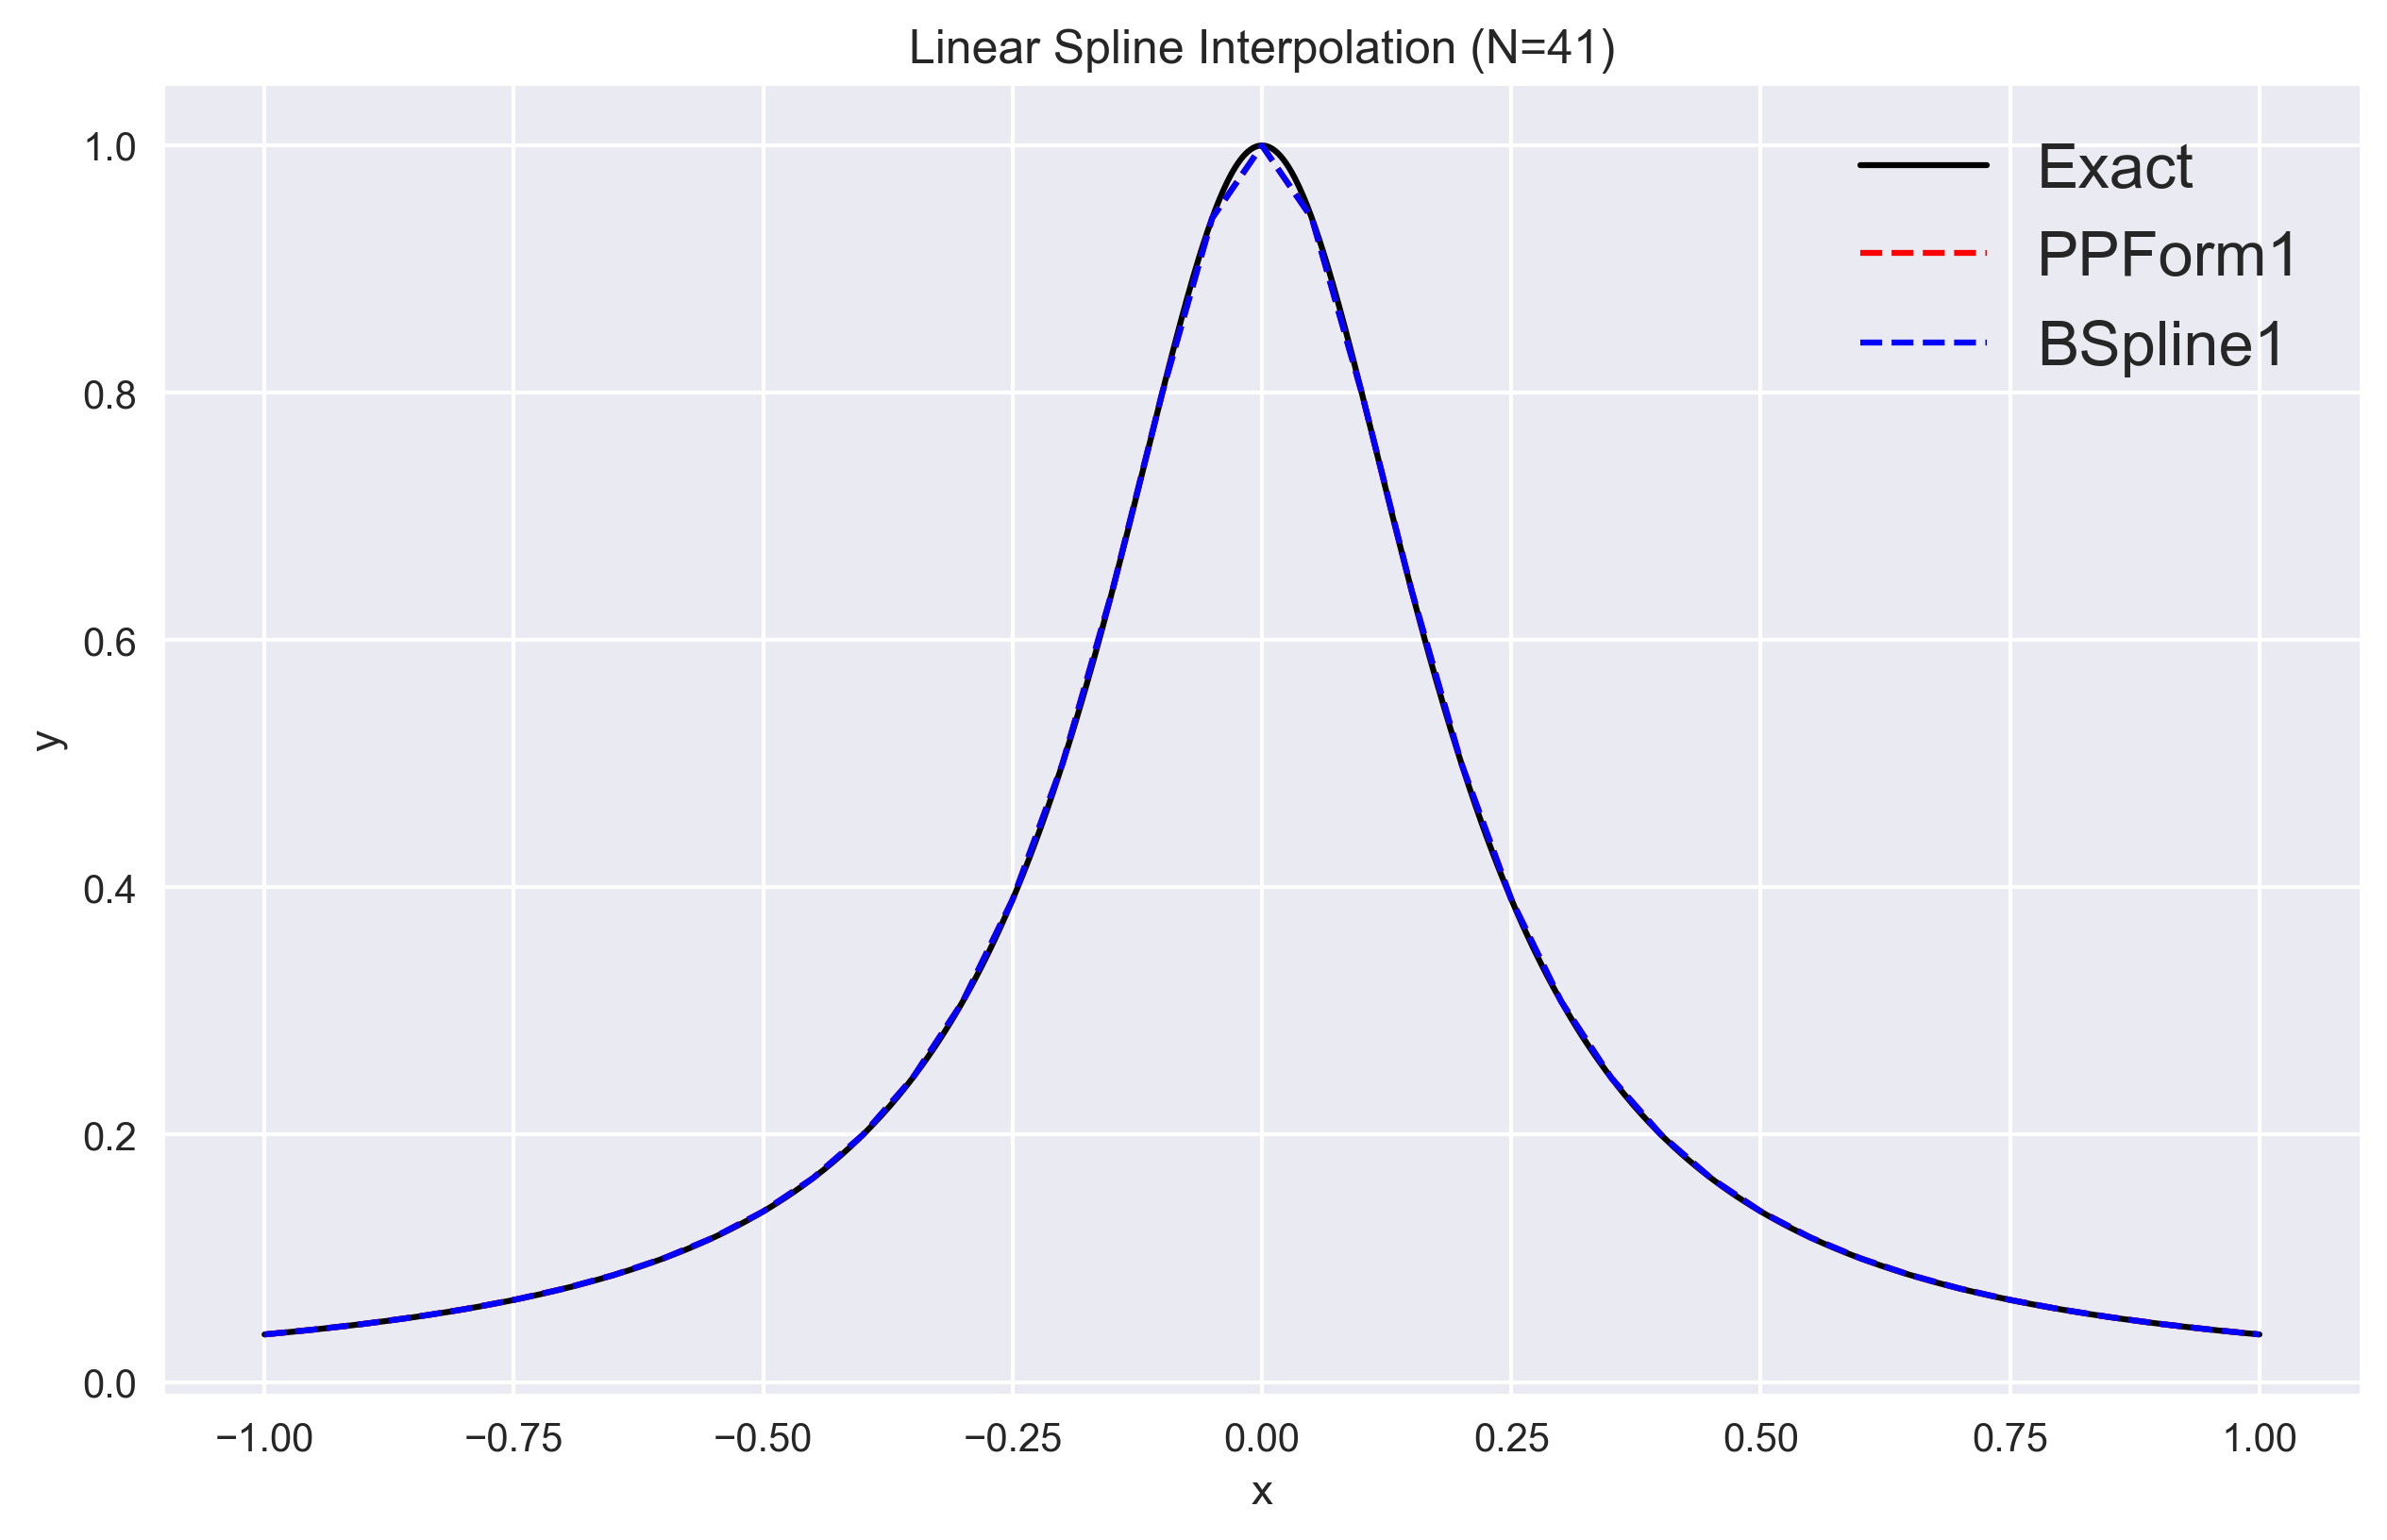
\includegraphics[width=0.45\textwidth]{../figure/problemA/linear_N41.png}   \\
    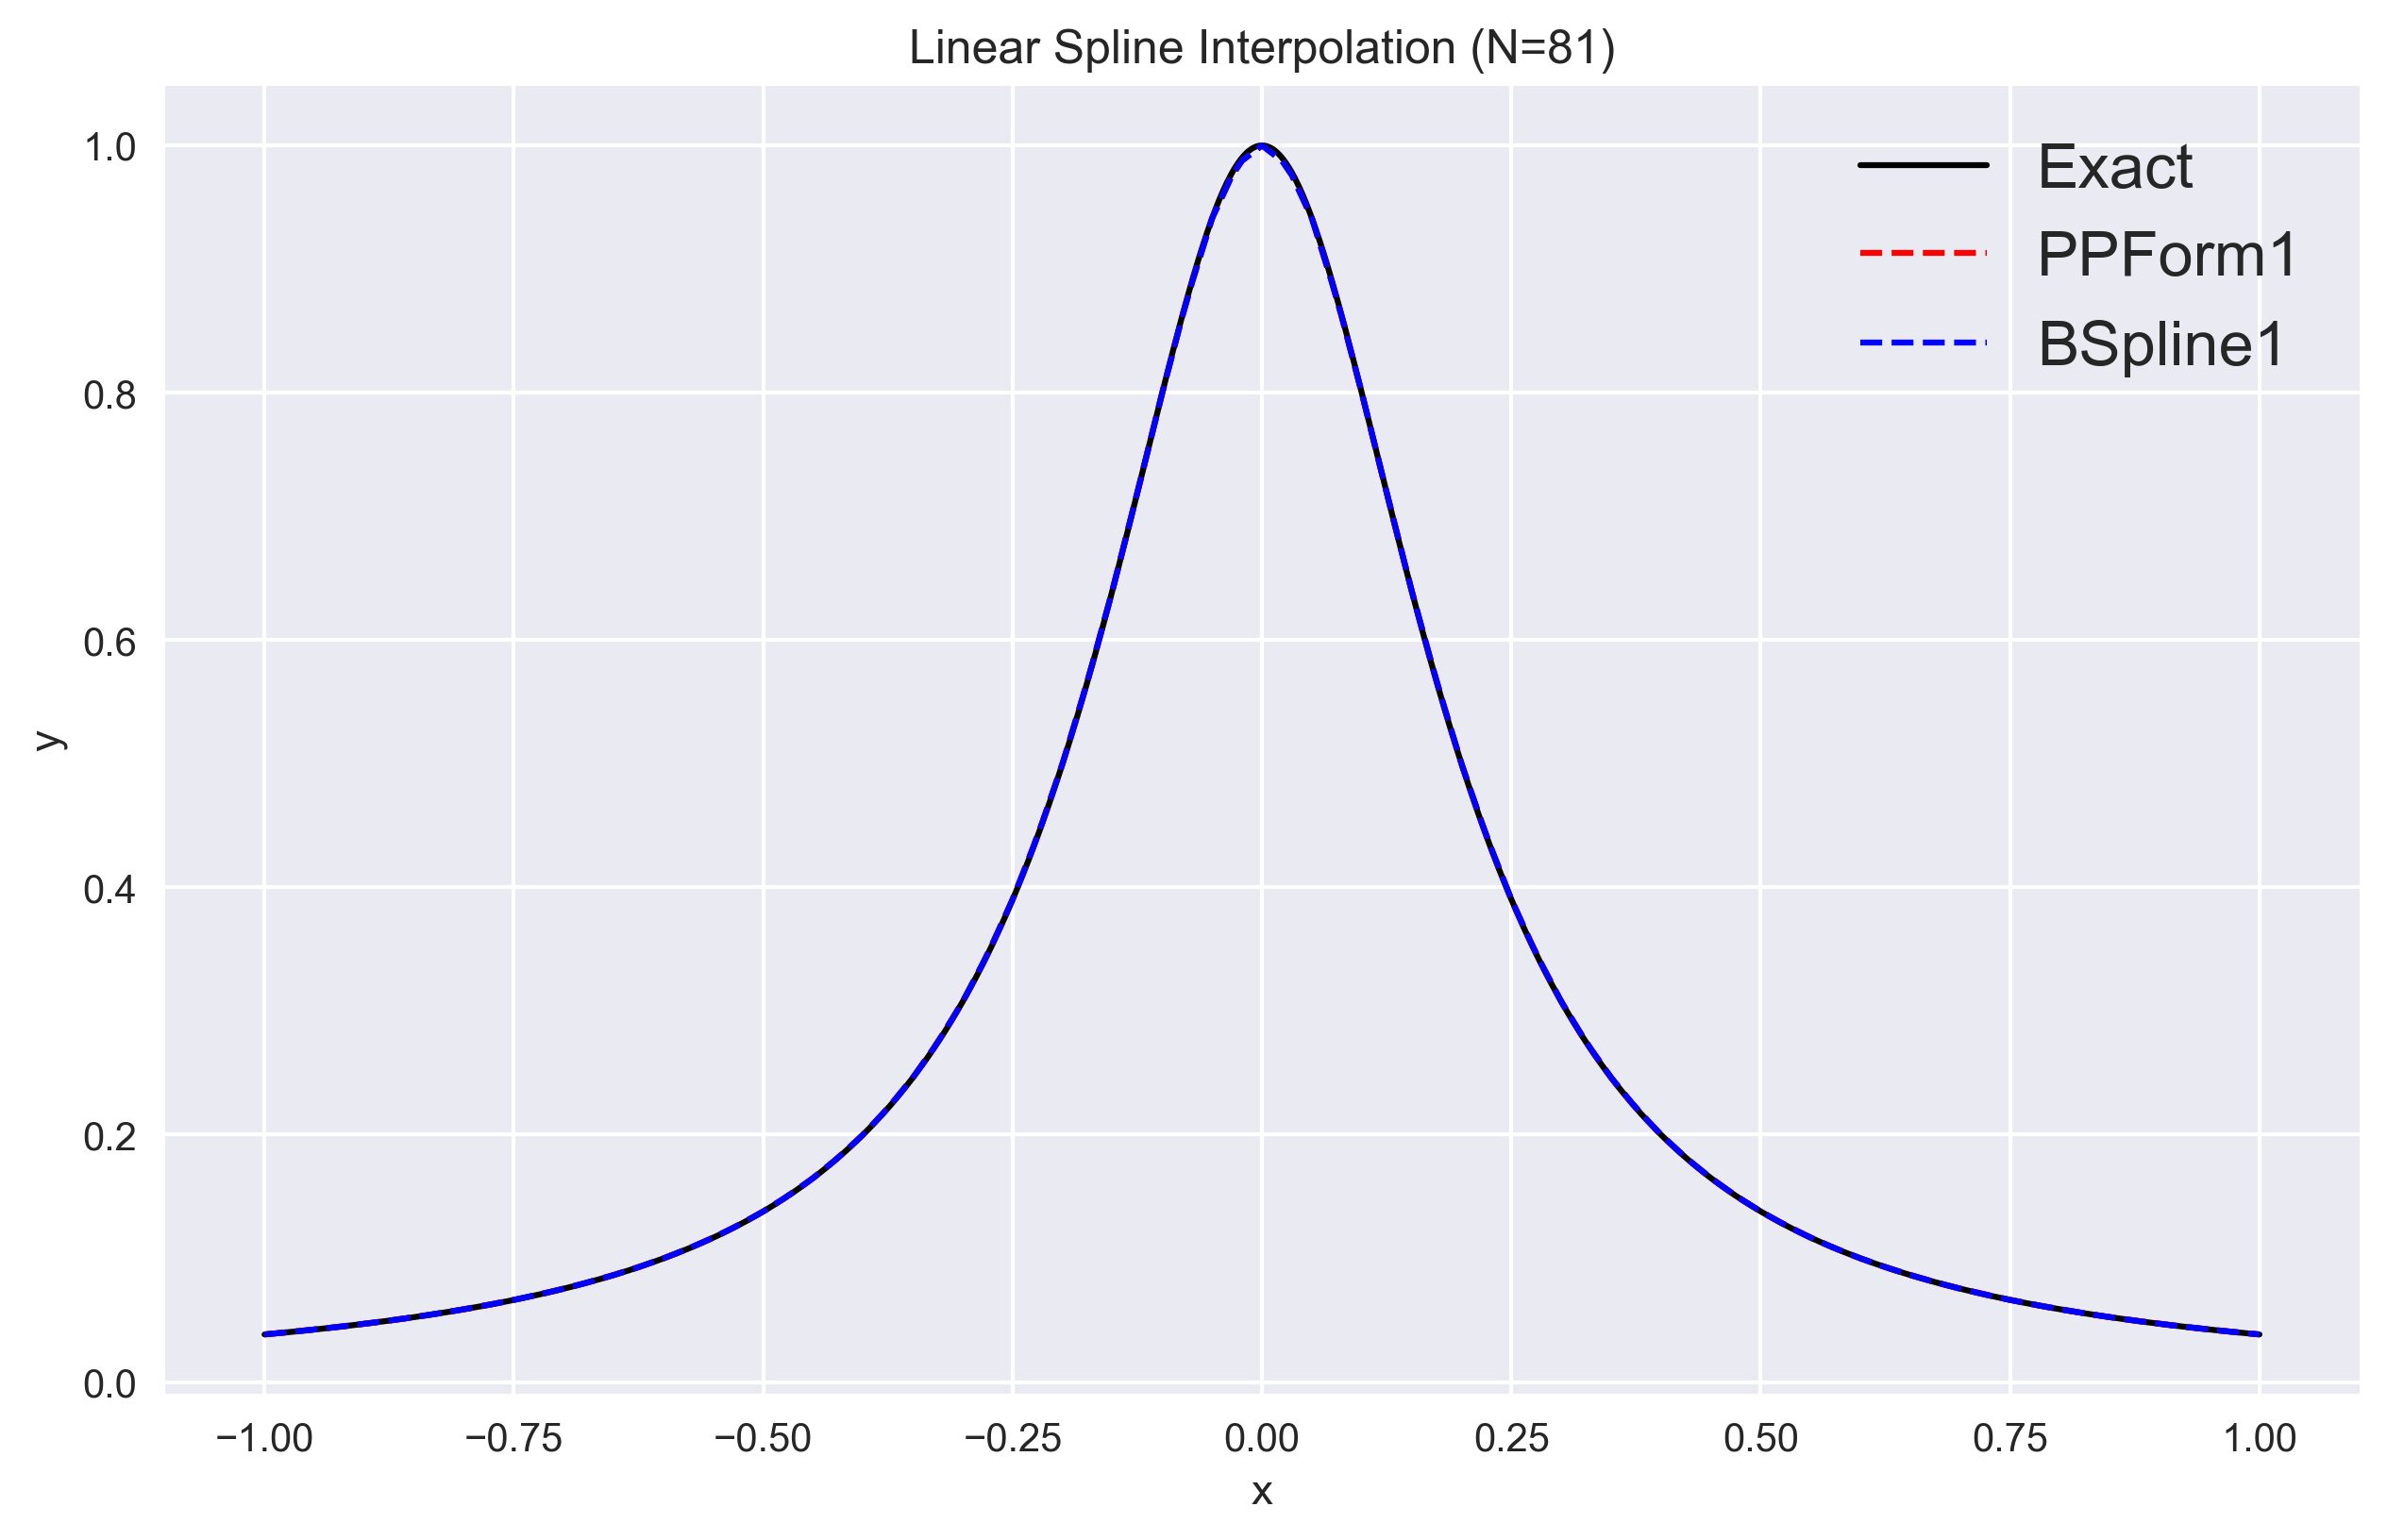
\includegraphics[width=0.45\textwidth]{../figure/problemA/linear_N81.png} &
  \end{tabular}
  \renewcommand{\figurename}{Fig.}
  \caption{Interpolation curves by linear splines}
  \label{fig:A_linear}
\end{figure}

From the above tests, it can be concluded that the two interpolation methods
can correctly implement linear spline functions under uniform node conditions
and cubic spline functions under various boundary conditions. A separate
program will be designed later to test interpolation under non-uniform node
conditions and periodic boundary conditions.

The max norm of the interpolation error vector at mid-points of the subintervals for cubic PPForm with complete boundary
conditions are as shown in Table.\ref{tab:maxnorm_error}:

\begin{table}[H]
  \centering
  \renewcommand{\tablename}{Table.}
  \caption{Max norm of the interpolation error vector at mid-points of the subintervals for cubic PPForm with complete boundary conditions}
  \label{tab:maxnorm_error}
  \begin{tabular}{|c|c|c|c|}
    \hline
    N  & Method  & BoundaryCondition & MaxNorm \\
    \hline
    6  & PPForm3 & COMPLETE          & 0.421705 \\
    11 & PPForm3 & COMPLETE          & 0.0205289 \\
    21 & PPForm3 & COMPLETE          & 0.00316894 \\
    41 & PPForm3 & COMPLETE          & 0.000275356 \\
    81 & PPForm3 & COMPLETE          & 1.609e-005 \\
    \hline
  \end{tabular}
\end{table}

The error and convergence rate data for cubic PPForm with complete boundary
conditions are as shown in Table.\ref{tab:maxerror_convergence}:
\begin{table}[H]
  \centering
  \renewcommand{\tablename}{Table.}
  \caption{Max errors and convergence rates for cubic PPForm with complete boundary conditions}
  \label{tab:maxerror_convergence}
  \begin{tabular}{|c|c|c|c|c|}
    \hline
    N  & Method  & BoundaryCondition & MaxError & ConvergenceRate \\
    \hline
    6  & PPForm3 & COMPLETE          & 0.421705 & 0.000000        \\
    11 & PPForm3 & COMPLETE          & 0.0219704 & -4.2626        \\
    21 & PPForm3 & COMPLETE          & 0.00318271 & -1.39362        \\
    41 & PPForm3 & COMPLETE          & 0.000277684 & -1.17291        \\
    81 & PPForm3 & COMPLETE          & 1.609e-005 & -1.0273        \\
    \hline
  \end{tabular}
\end{table}

The convergence rate is calculated using the formula:
\[
  \text{rate} = \frac{\log\left(\frac{\text{max\_error\_current}}{\text{max\_error\_previous}}\right)}{\log\left(\frac{\frac{2}{N_{\text{current}} - 1}}{\frac{2}{N_{\text{previous}} - 1}}\right)}
\]
where \(\text{max\_error\_current}\) and \(\text{max\_error\_previous}\) are
the maximum errors for the current and previous number of interpolation points
\(N_{\text{current}}\) and \(N_{\text{previous}}\), respectively.

To illustrate this relationship, we can plot \(N\) against the maximum error on
a logarithmic scale. The least squares fit of the error data in logarithmic
coordinates calculated by \verb|src\problemA\plotA_leastSquare.py| is also
shown. It is depicted in Fig.\ref{fig:N_vs_maxerror}.
\begin{figure}[H]
  \centering
  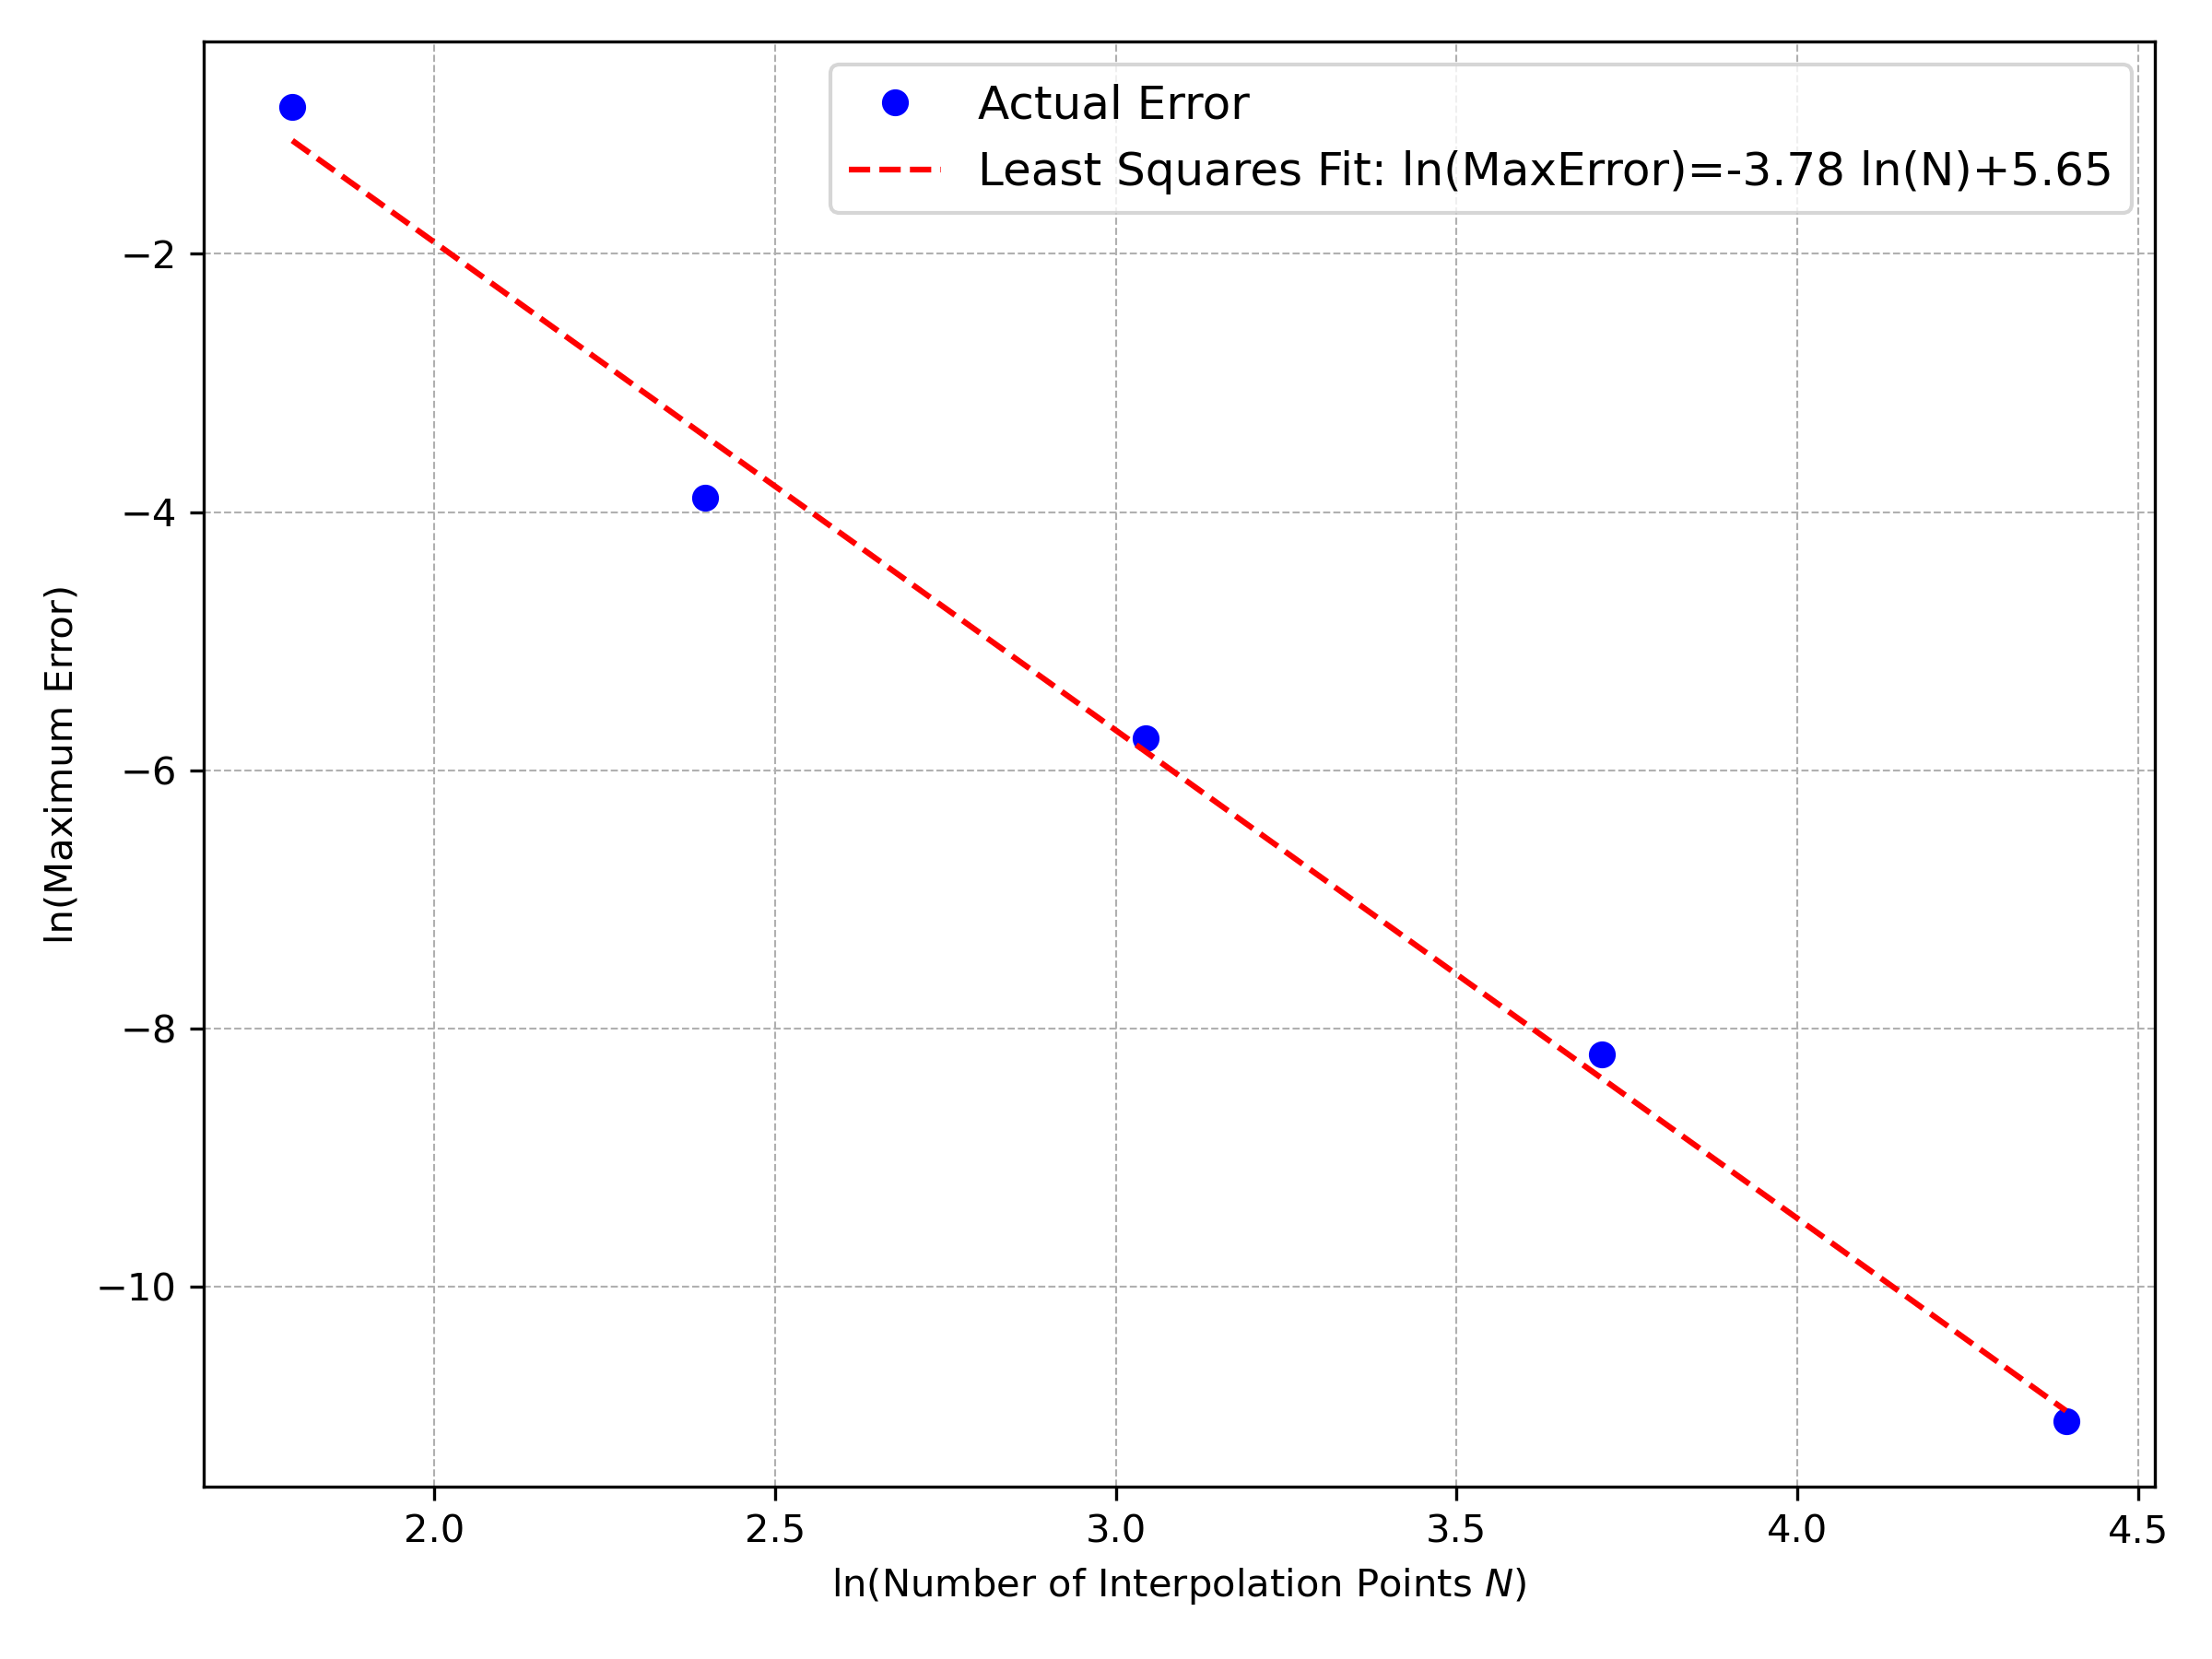
\includegraphics[width=0.8\textwidth]{../figure/problemA/lnN_vs_lnMaxError.png}
  \renewcommand{\figurename}{Fig.}
  \caption{Log-log plot of \(N\) vs. Maximum Error for cubic PPForm splines with complete boundary conditions}
  \label{fig:N_vs_maxerror}
\end{figure}

The relationship between \(N\) and the maximum error can be analyzed from
several aspects:

\begin{enumerate}
  \item \textbf{Small Dataset Behavior (N $\leq$ 11):} \\
        For small \(N\), the convergence rate is notably high (around -4.36), indicating rapid error reduction. This is particularly evident in the transition from \(N=6\) to \(N=11\), where the maximum error drops dramatically from 0.421705 to 0.020529.

  \item \textbf{Large Dataset Behavior (N $\geq$ 41):} \\
        As \(N\) increases, the convergence rate gradually stabilizes near -1, suggesting a more moderate decrease in error. For example, from \(N=41\) to \(N=81\), the convergence rate is approximately -1.02426.
\end{enumerate}

The least squares fit of the error data in logarithmic coordinates yields:
\[
  \ln(\text{MaxError})=-3.78\ln(N)+5.65
\]
or equivalently in exponential form:
\[
  \text{MaxError} = e^{5.65}N^{-3.78} \approx 284.290N^{-3.78}
\]
This confirms that the error decreases approximately as \(O(N^{-3.77})\).

\section{Problem C}
Compile and run the program \verb|C.cpp|. Its output includes the values of the interpolation curves for plotting. The data stores in the directory \verb|output\problemC|.

Compile and run the program \verb|plotC.py| to plot the interpolation curves
and the original function. The figure is shown in
Fig.\ref{fig:BSpline_interpolation_C}.

\begin{figure}[H]
  \centering
  \begin{tabular}{c}
    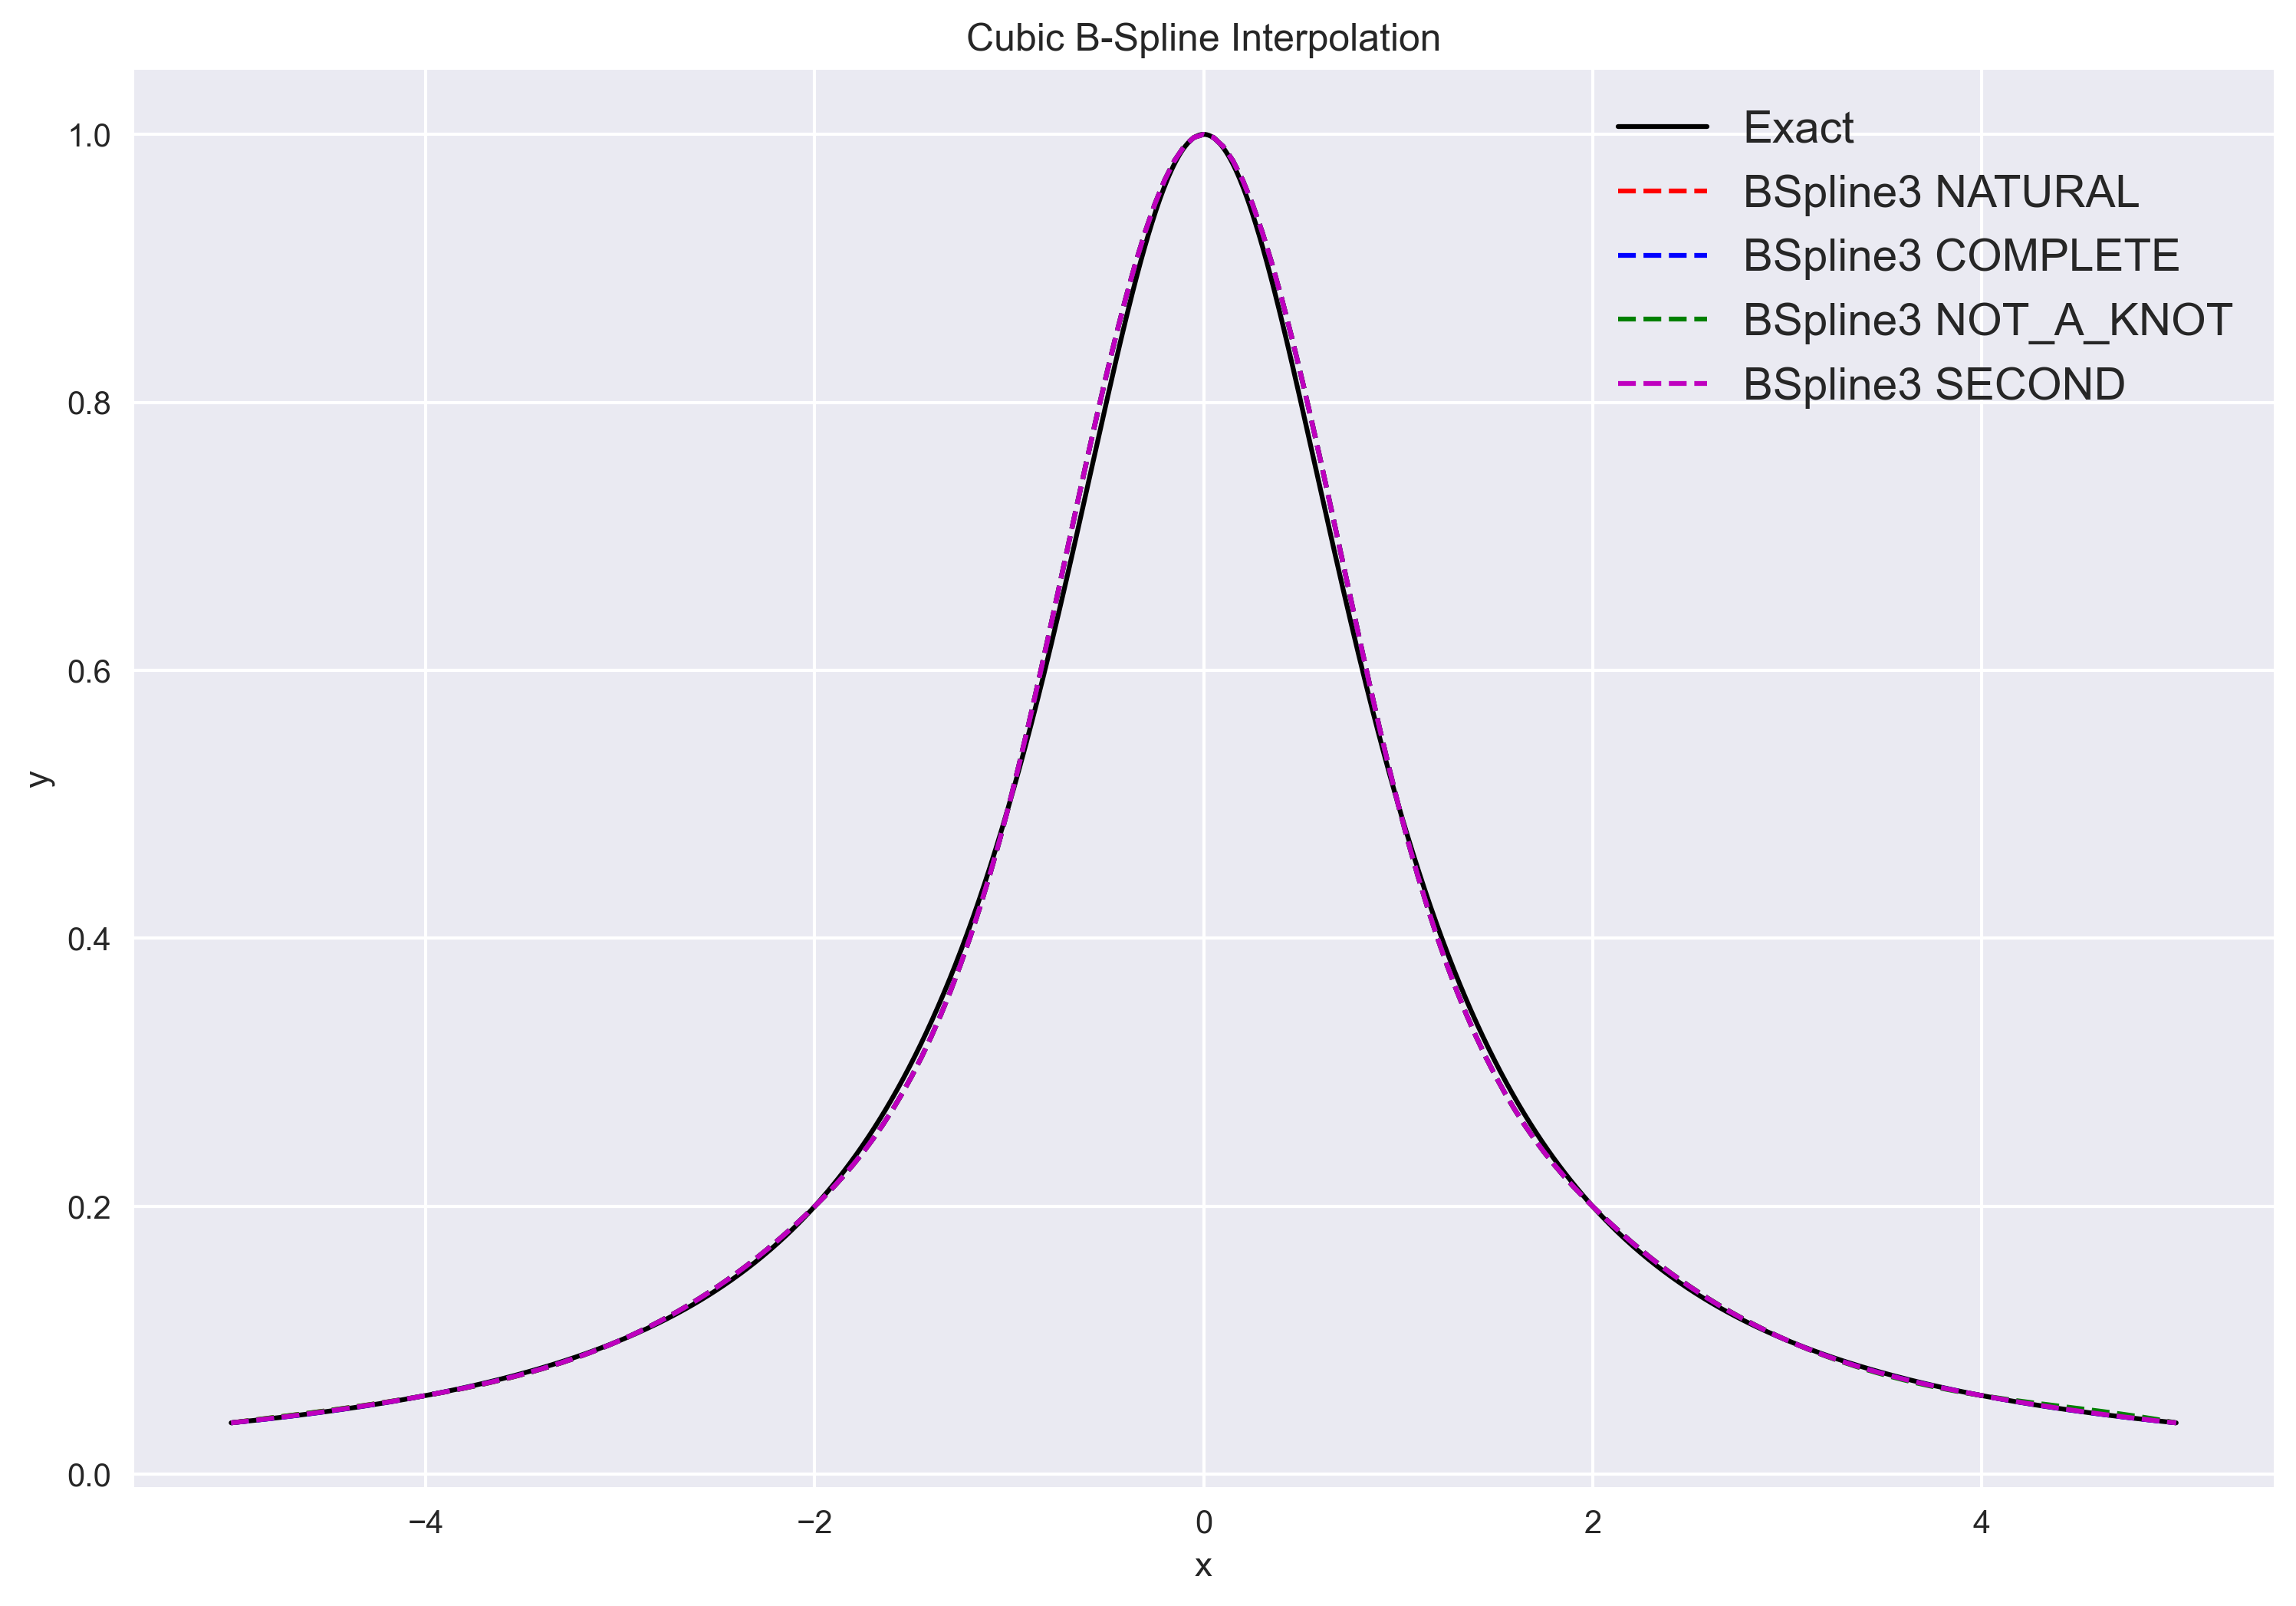
\includegraphics[width=0.6\textwidth]{../figure/problemC/Cubic_BSpline_interpolation.png} \\
    \includegraphics[width=0.6\textwidth]{../figure/problemC/Quadratic_BSpline_interpolation.png}
  \end{tabular}
  \renewcommand{\figurename}{Fig.}
  \caption{Quadratic and cubic BSpline interpolation for Problem C}
  \label{fig:BSpline_interpolation_C}
\end{figure}

The program tests quadratic B-spline curve fitting for the target function and
cubic B-spline curve fitting under various boundary conditions and linear
B-spline curve fitting.

The implementation of the quadratic B-spline curve follows the relevant
theorems in the textbook. In the actual implementation, it is ensured that the
quadratic spline passes through all control points and that the first
derivative is continuous at the internal nodes, except for the first two and
the last two nodes.

The linear B-spline curve uses the same interpolation points as the cubic
B-spline, mainly to test whether the B-spline linear interpolation can be
correctly implemented. The figure is shown in
Fig.\ref{fig:Linear_BSpline_interpolation_C}.

\begin{figure}[H]
  \centering
  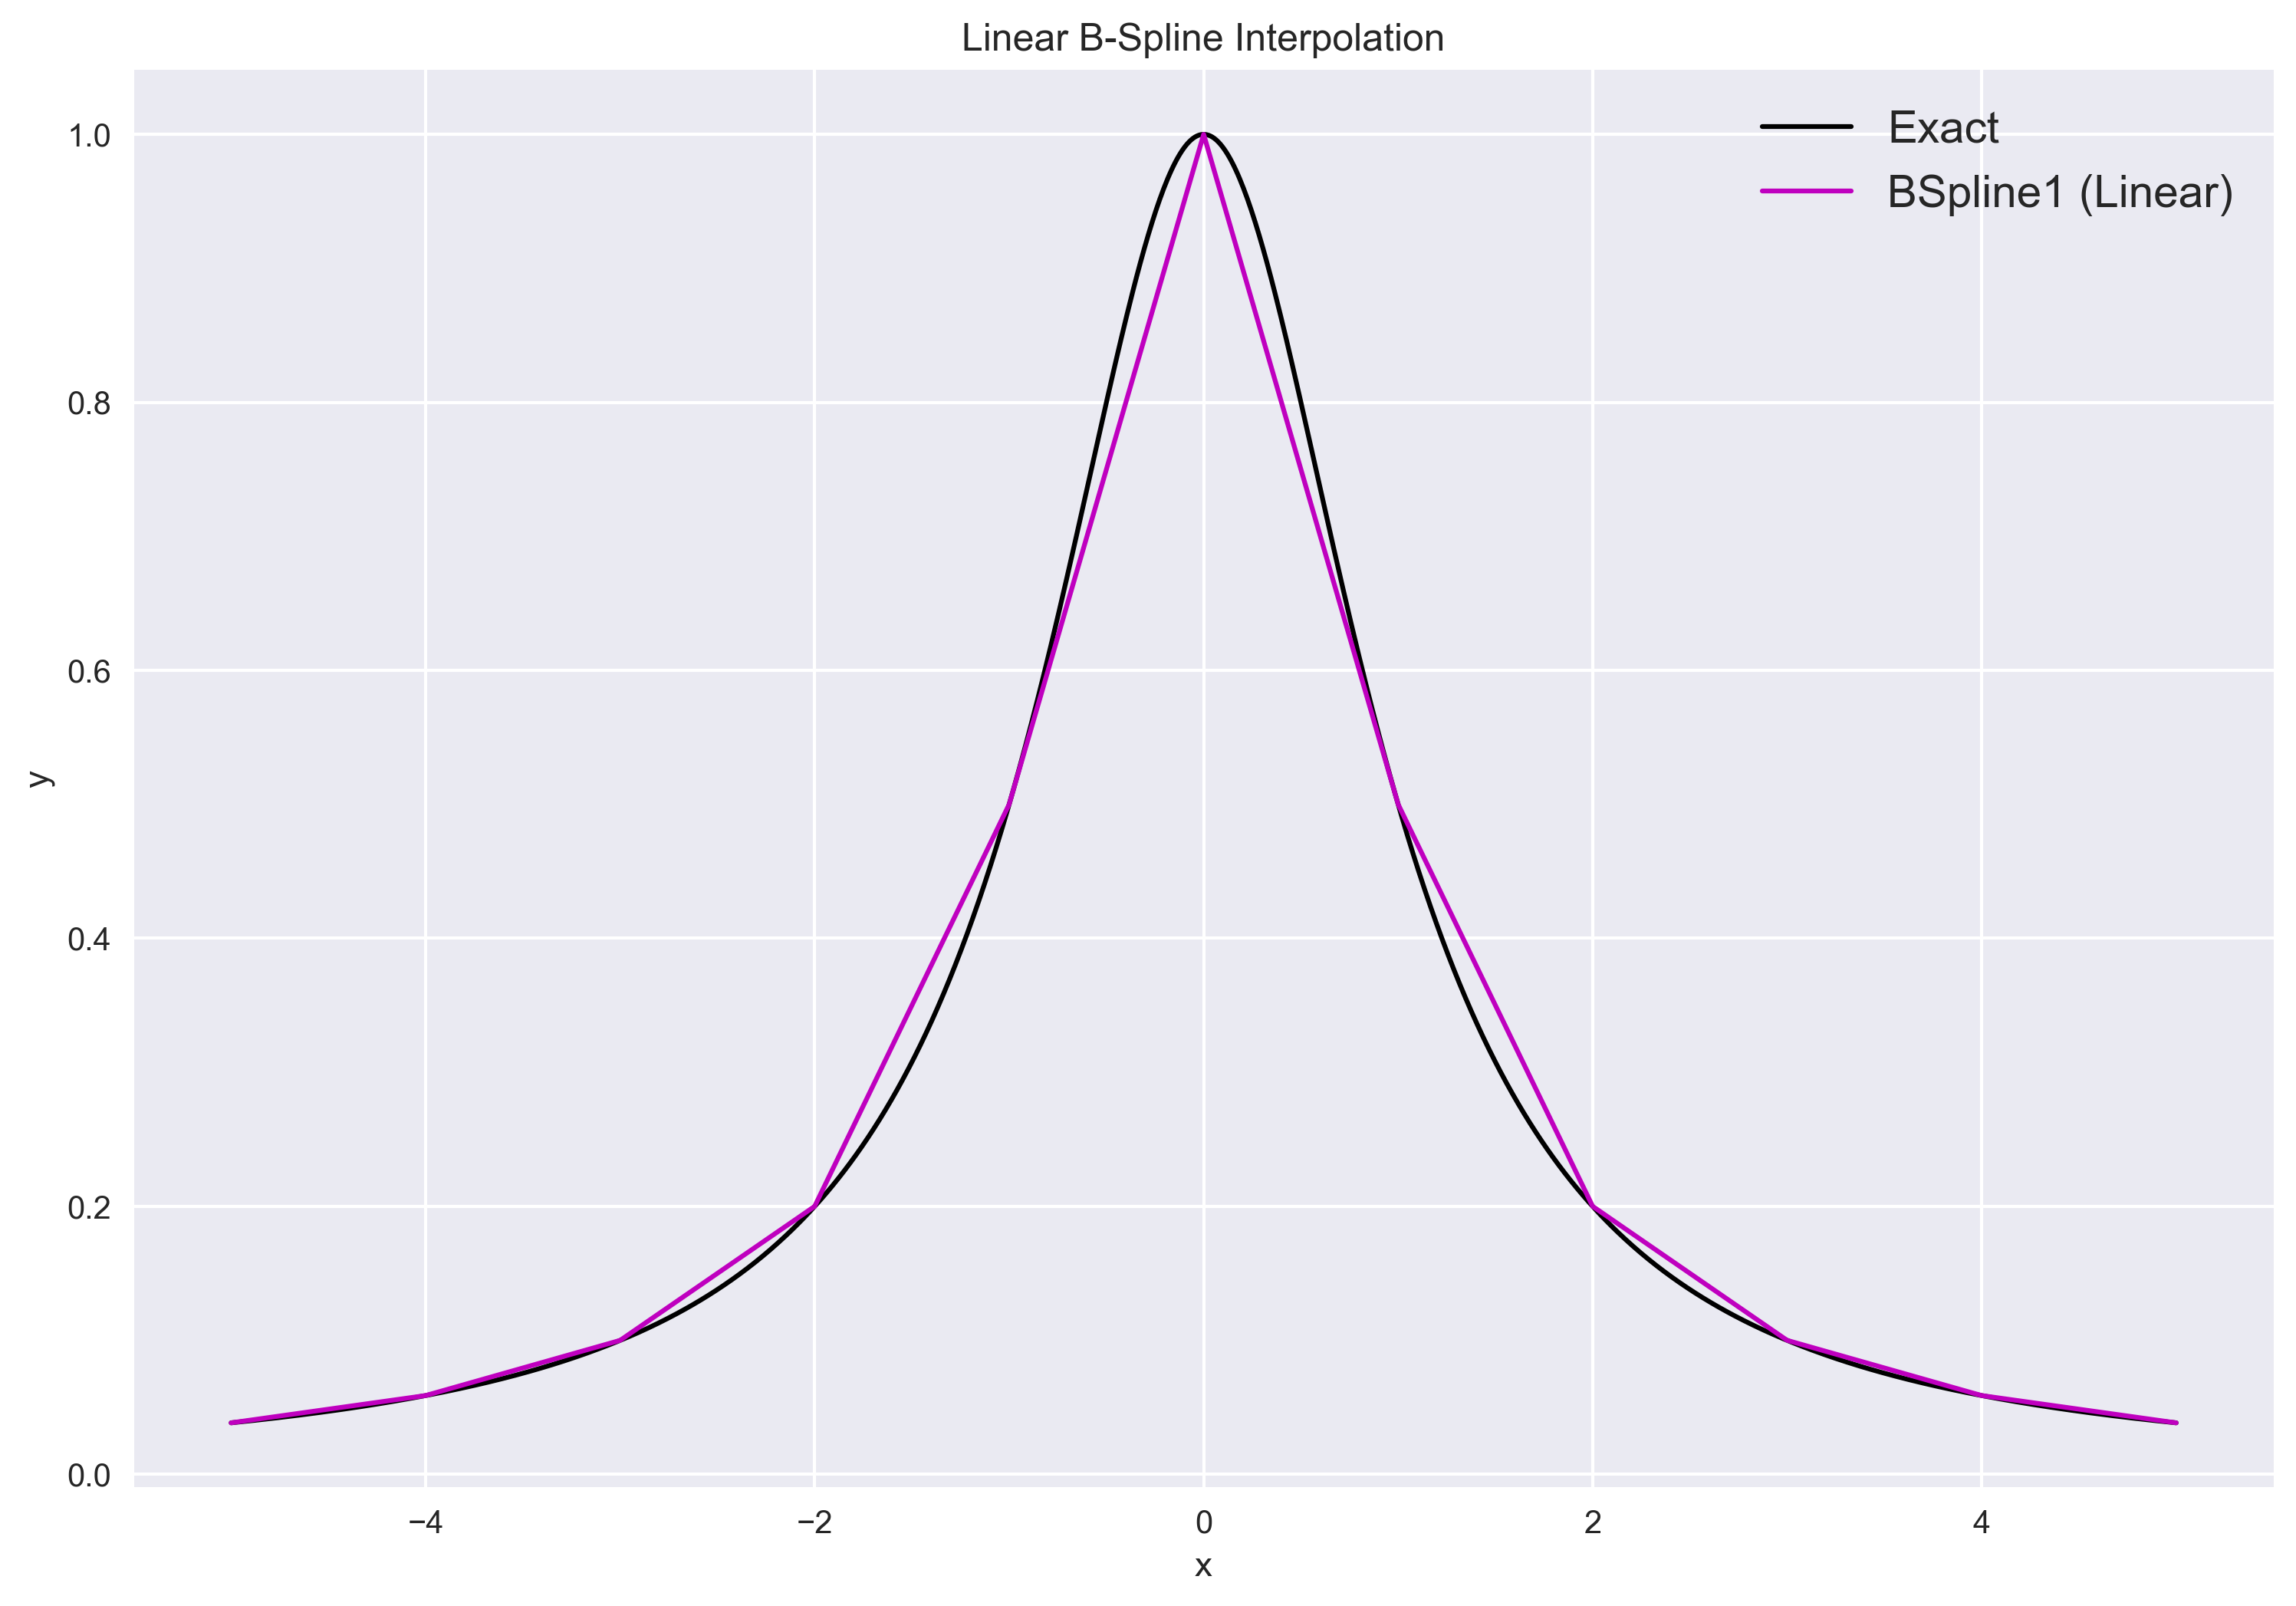
\includegraphics[width=0.6\textwidth]{../figure/problemC/Linear_BSpline_interpolation.png}
  \renewcommand{\figurename}{Fig.}
  \caption{Linear BSpline interpolation for Problem C}
  \label{fig:Linear_BSpline_interpolation_C}
\end{figure}

As can be seen from the figure, the fitting effect of the quadratic B-spline
curve is worse than that of the cubic B-spline curve. This is because the
locality of the quadratic spline is stronger than that of the cubic spline,
which weakens the fitting effect. The linear B-spline curve fitting effect is
also worse than the cubic B-spline curve, which is consistent with the
theoretical analysis.

\section{Problem D}
Compile and run the program \verb|D.cpp|. Its output includes the error data of specific points and max errors data for different B-spline methods and the values of the interpolation curves for plotting. The data stores in the directory \verb|output\problemD|.

In the bspline package, the relevant functions for the 2nd-order cardinal
B-spline have been implemented separately. Since the 3rd-order cardinal
B-spline required by the problem can be implemented by the existing 3rd-order
B-spline with arbitrary nodes, the 3rd-order cardinal B-spline has not been
implemented separately in the program.

I added first-order B-splines to test whether the first-order B-spline
interpolation algorithm is correct, using the same interpolation points as the
third-order B-splines.

The error data of specific points for different B-spline methods is shown in
Table.\ref{tab:error_data}.

\begin{table}[H]
  \centering
  \renewcommand{\tablename}{Table.}
  \caption{Error Data for Different B-spline Methods}
  \label{tab:error_data}
  \pgfplotstabletypeset[
    col sep=comma,
    string type,
    columns/x/.style={
        column name=x,
        column type={|c}
      },
    columns/BSpline1/.style={
        column name=BSpline1,
        column type={|c}
      },
    columns/BSpline2/.style={
        column name=BSpline2,
        column type={|c}
      },
    columns/BSpline3_NATURAL/.style={
        column name=\makecell{BSpline3\\NATURAL},
        column type={|c}
      },
    columns/BSpline3_COMPLETE/.style={
        column name=\makecell{BSpline3\\COMPLETE},
        column type={|c}
      },
    columns/BSpline3_NOT_A_KNOT/.style={
        column name=\makecell{BSpline3\\NOT A KNOT},
        column type={|c}
      },
    columns/BSpline3_SECOND/.style={
        column name=\makecell{BSpline3\\SECOND},
        column type={|c|} % Ensures the last column has a right border
      },
    every head row/.style={
        before row=\hline,
        after row=\hline
      },
    every last row/.style={
        after row=\hline
      },
  ]{../output/problemD/error.csv}
\end{table}

It was observed that some of the errors close to machine precision. At -3.0 and
3.0, the error between the first-order B-spline and the actual function is
close to machine precision $2.2e^{-16}$. This is because these points are
control points, and the curve must pass through these points. At -3.5, -0.5,
0.5, and 3.5, the error between the second-order B-spline and the actual
function is close to machine precision $2.2e^{-16}$, for the same reason.

Additionally, it may also be due to the inevitable floating-point errors in the
computer's calculation when computing the actual function values, the fitted
curve values and the interpolation points.

From the max errors data shown in Table.\ref{tab:maxerror_data} and the images
of the interpolation curve shown in Fig.\ref{fig:BSpline_interpolation_C} and
Fig.\ref{fig:Linear_BSpline_interpolation_C}, it can be seen that under the
same node conditions, the cubic B-spline interpolation is more accurate than
the linear B-spline interpolation. Comparing the quadratic cardinal B-spline
with the cubic cardinal B-spline, the cubic cardinal B-spline provides a better
fitting effect.

\begin{table}[H]
  \centering
  \renewcommand{\tablename}{Table.}
  \caption{Max Errors for Different B-spline Methods}
  \label{tab:maxerror_data}
  \pgfplotstabletypeset[
    col sep=comma,
    string type,
    columns/Method/.style={
        column name=Method,
        column type={|c}
      },
    columns/BSpline1/.style={
        column name=BSpline1,
        column type={|c}
      },
    columns/BSpline2/.style={
        column name=BSpline2,
        column type={|c}
      },
    columns/BSpline3_NATURAL/.style={
        column name=\makecell{BSpline3\\NATURAL},
        column type={|c}
      },
    columns/BSpline3_COMPLETE/.style={
        column name=\makecell{BSpline3\\COMPLETE},
        column type={|c}
      },
    columns/BSpline3_NOT_A_KNOT/.style={
        column name=\makecell{BSpline3\\NOT A KNOT},
        column type={|c}
      },
    columns/BSpline3_SECOND/.style={
        column name=\makecell{BSpline3\\SECOND},
        column type={|c|} % Ensures the last column has a right border
      },
    every head row/.style={
        before row=\hline,
        after row=\hline
      },
    every last row/.style={
        after row=\hline
      },
  ]{../output/problemD/maxerror.csv}
\end{table}

\section{Problem E}
Compile and run the program \verb|E.cpp|. Its output includes max errors data for B-spline in \verb|maxerror.csv| and PPForm methods of different boundary conditions and the values of the fitted and actual curves for plotting. It also outputs a file \verb|compare.csv| that compares whether the curves obtained with the same interpolation points and boundary conditions under equidistant node conditions are consistent between PPForm and B-spline methods. The data is stored in the directory \verb|output\problemE|.

Compile and run the program \verb|plotE.py| to plot the interpolation curves
and the original function. The figures are stored in the directory
\verb|figure\problemE|.

Compile and run the program \verb|plotE_error.py| to plot the least squares fit
of the maximum errors of different curves under different methods with
equidistant nodes. The cumulative chordal length method's error is not
calculated because there is no good method to compute it. The error of 2D
curves is calculated using Euclidean distance, and the error on the 3D unit
sphere is calculated using spherical angular distance.

Reviewing the problem, the required curves are as follows: The heart-shaped
curve \(r_1\) is given by $$ r_1(t)=(x(t),y(t))=\left(\sqrt{3} \sin t, \frac{2
    \sqrt{3}}{3} \cos t + \frac{2}{3} \sqrt{\sqrt{3} |\sin t|}\right),\ t\in
  [0,2\pi]. $$

The spiral curve \(r_2\) is given by $$ r_2(t)=(x(t),y(t))=(\sin t+t\cos t,\cos
  t-t\sin t),\ t\in[0,6\pi]. $$

The curve \(r_3\) is given by $$
  r_3(t)=(x(t),y(t),z(t))=(\sin(u(t))\cos(v(t)),\sin u(t)\sin v(t),\cos u(t)),\
  t\in[0,2\pi] $$ where \(u(t)=\cos t,\:v(t)=\sin t\).

According to the coordinate data files of the fitted curves, as shown in
Table.\ref{tab:compare_ppform_bspline}, the curves obtained by PPForm and
B-spline methods with the same interpolation points and boundary conditions are
consistent within the allowable error range.

\begin{table}[H]
  \centering
  \renewcommand{\tablename}{Table.}
  \caption{Comparison of PPForm and B-Spline Methods}
  \label{tab:compare_ppform_bspline}
  \pgfplotstabletypeset[
    col sep=comma,
    string type,
    columns/curve/.style={
        column name=Curve,
        column type={|c}
      },
    columns/N/.style={
        column name=N,
        column type={|c}
      },
    columns/boundary/.style={
        column name=Boundary,
        column type={|c},
        string replace*={_}{\_}
      },
    columns/isTheSame/.style={
        column name=Is The Same,
        column type={|c|}, % Ensures the last column has a right border
        string replace*={_}{\_}
      },
    every head row/.style={
        before row=\hline,
        after row=\hline
      },
    every last row/.style={
        after row=\hline
      },
  ]{../output/problemE/compare.csv}
\end{table}

Therefore, the following discussion only considers the fitted curves under the
BSpline method.

The least squares fit of the maximum errors of different curves under different
methods with equidistant nodes is shown in Fig.\ref{fig:leastSquare_fit}.

\begin{figure}[H]
  \centering
  \begin{tabular}{cc}
    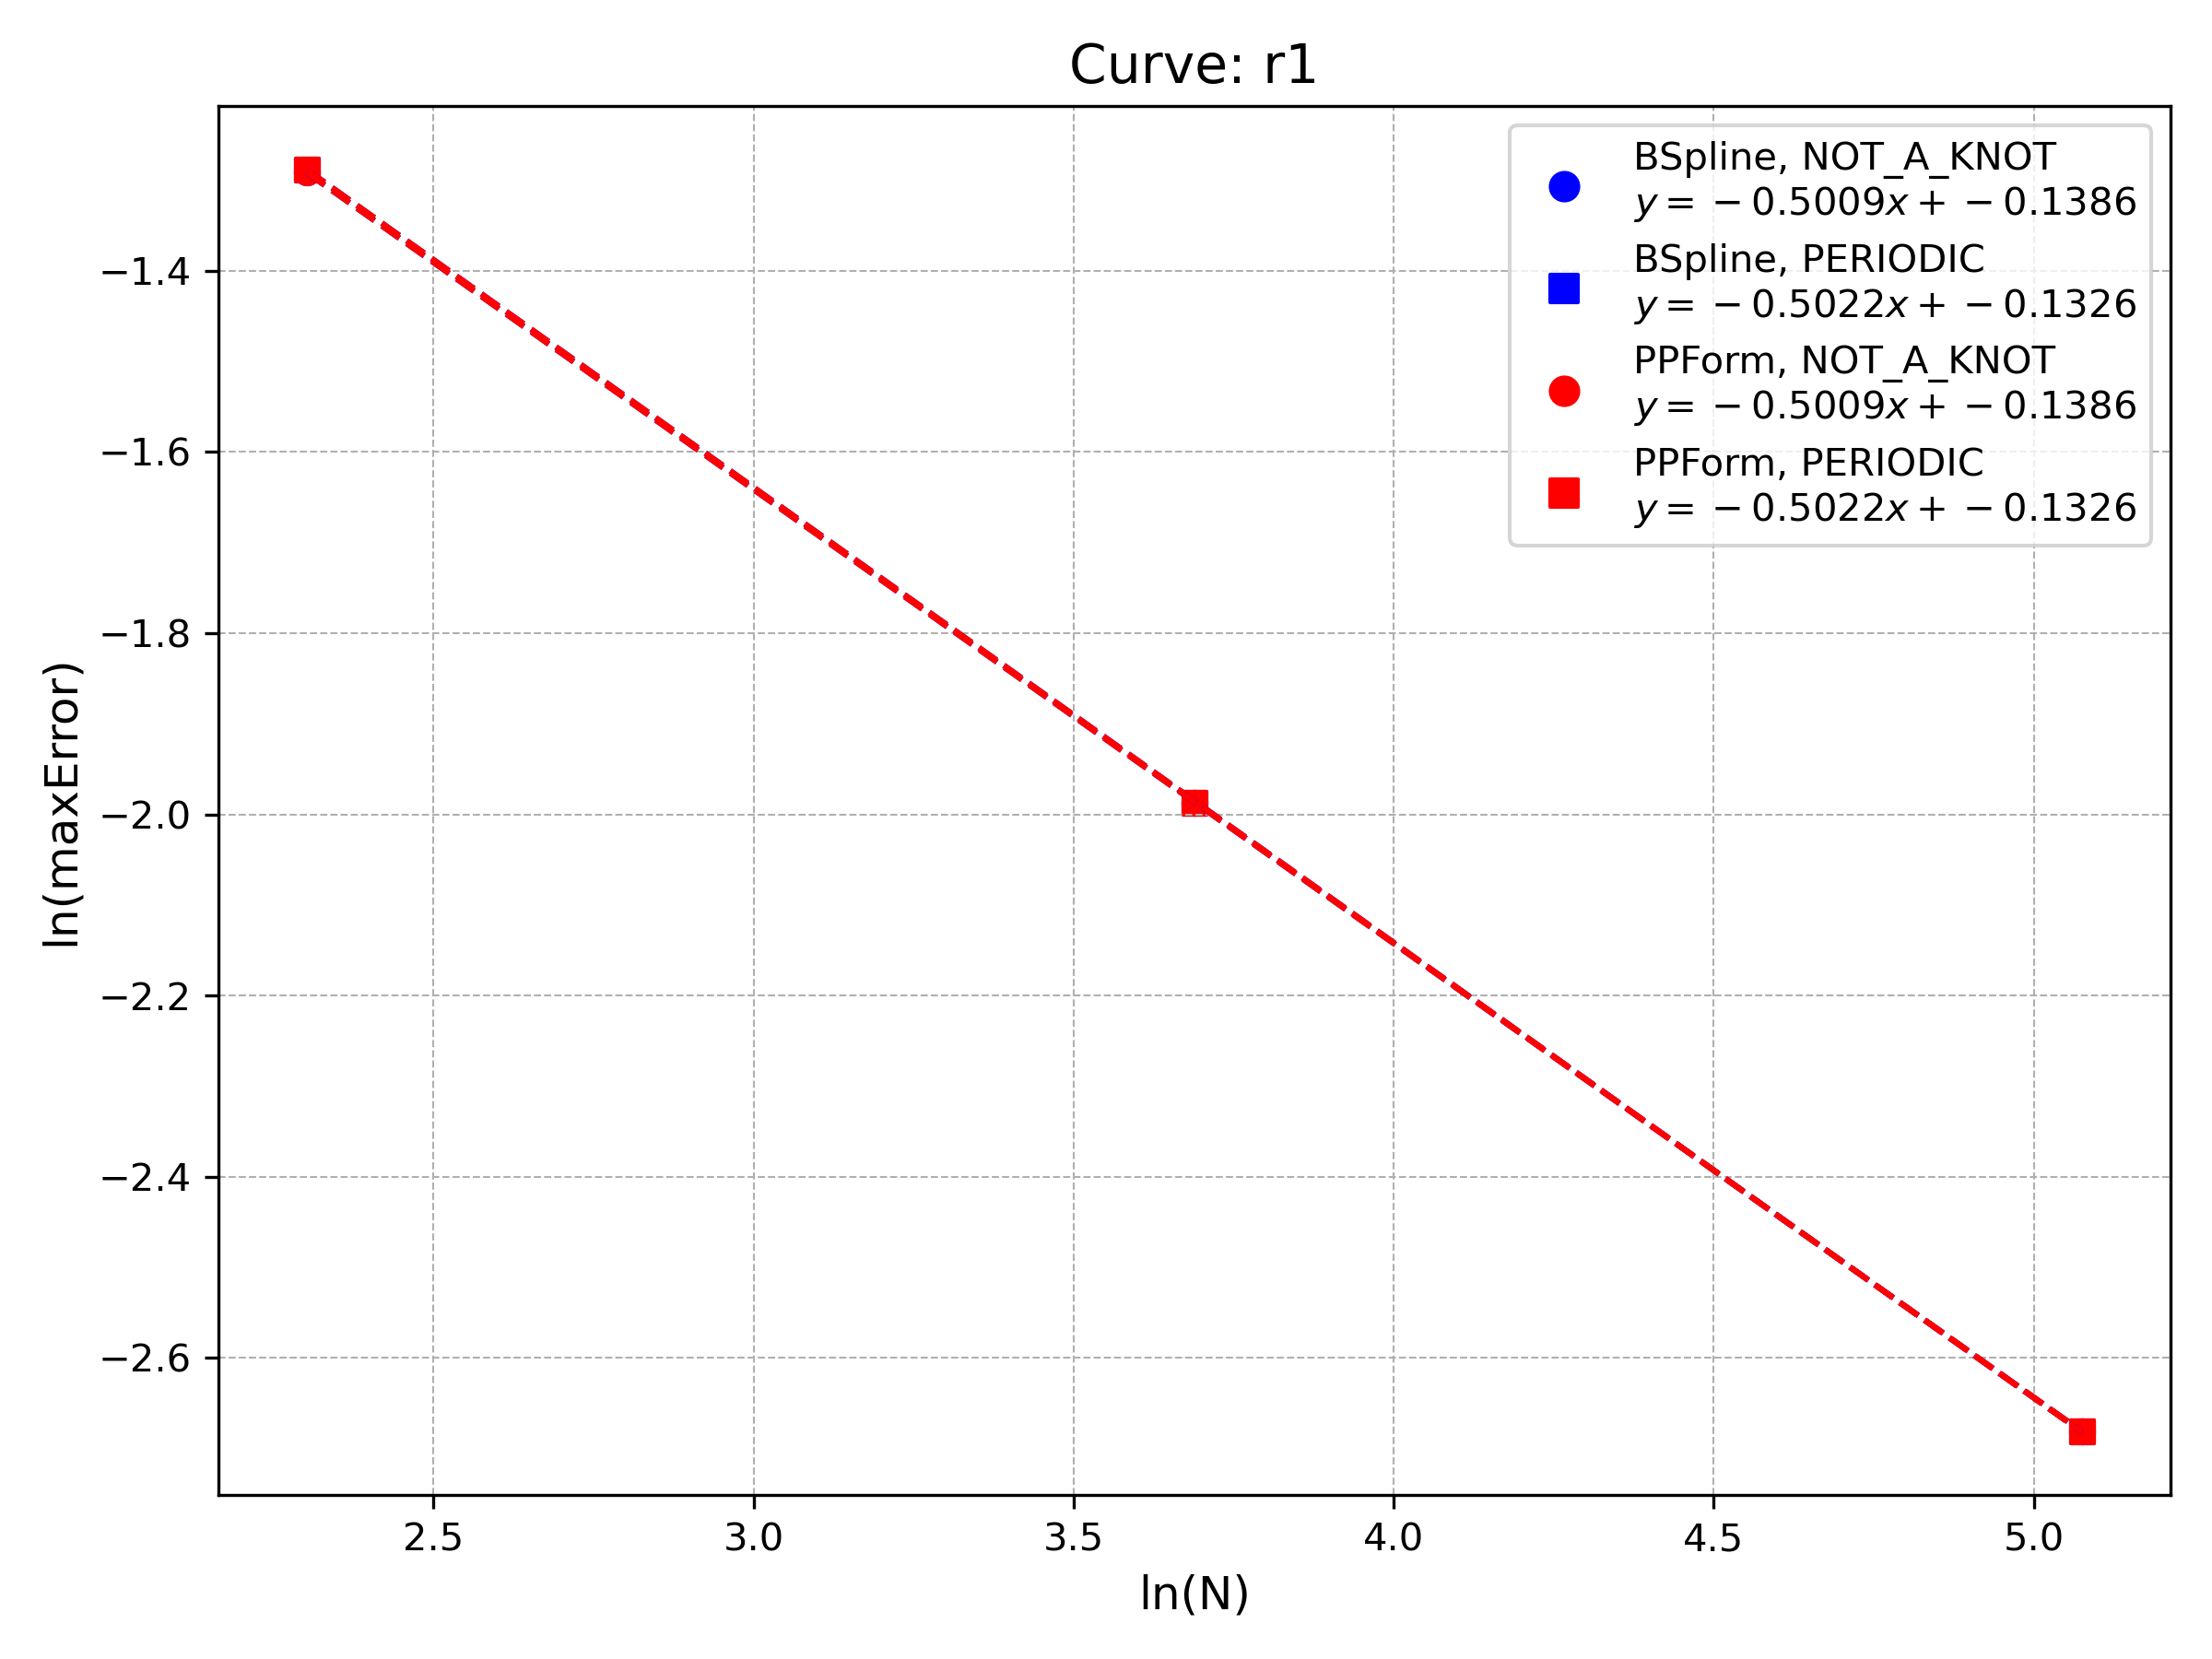
\includegraphics[width=0.45\textwidth]{../figure/problemE/r1_lnMaxError_vs_lnN.png} &
    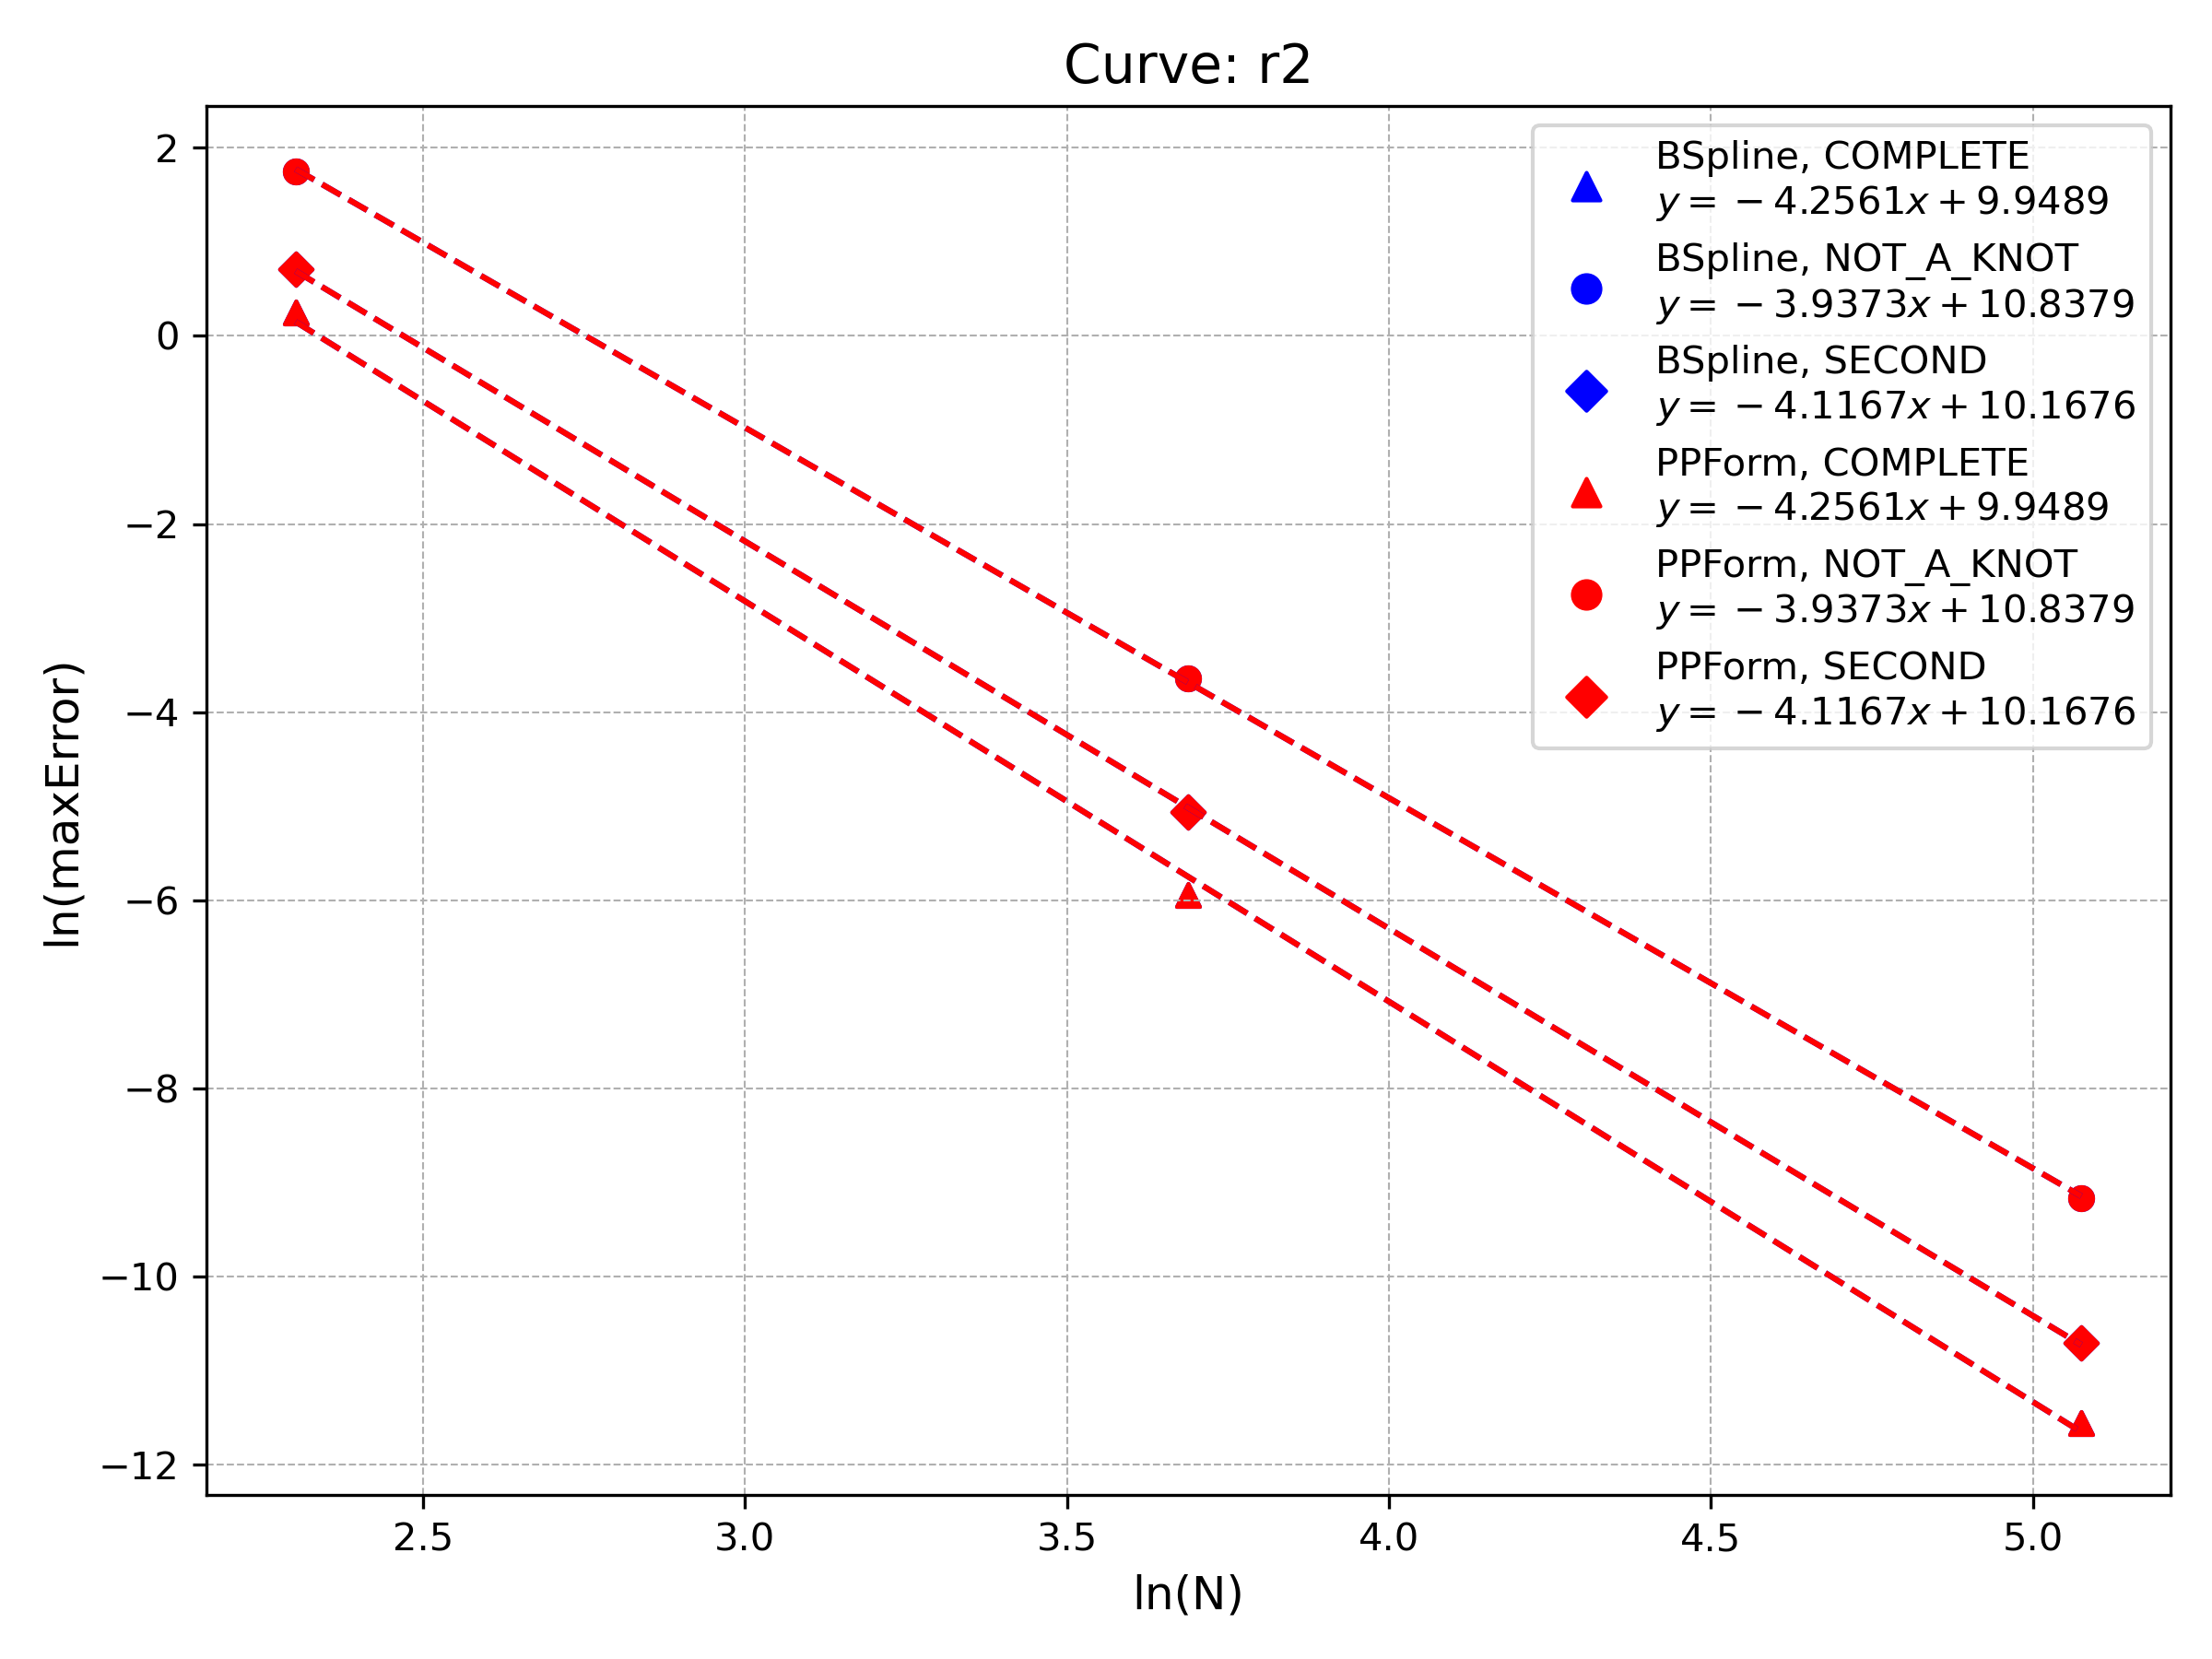
\includegraphics[width=0.45\textwidth]{../figure/problemE/r2_lnMaxError_vs_lnN.png}   \\
    \multicolumn{2}{c}{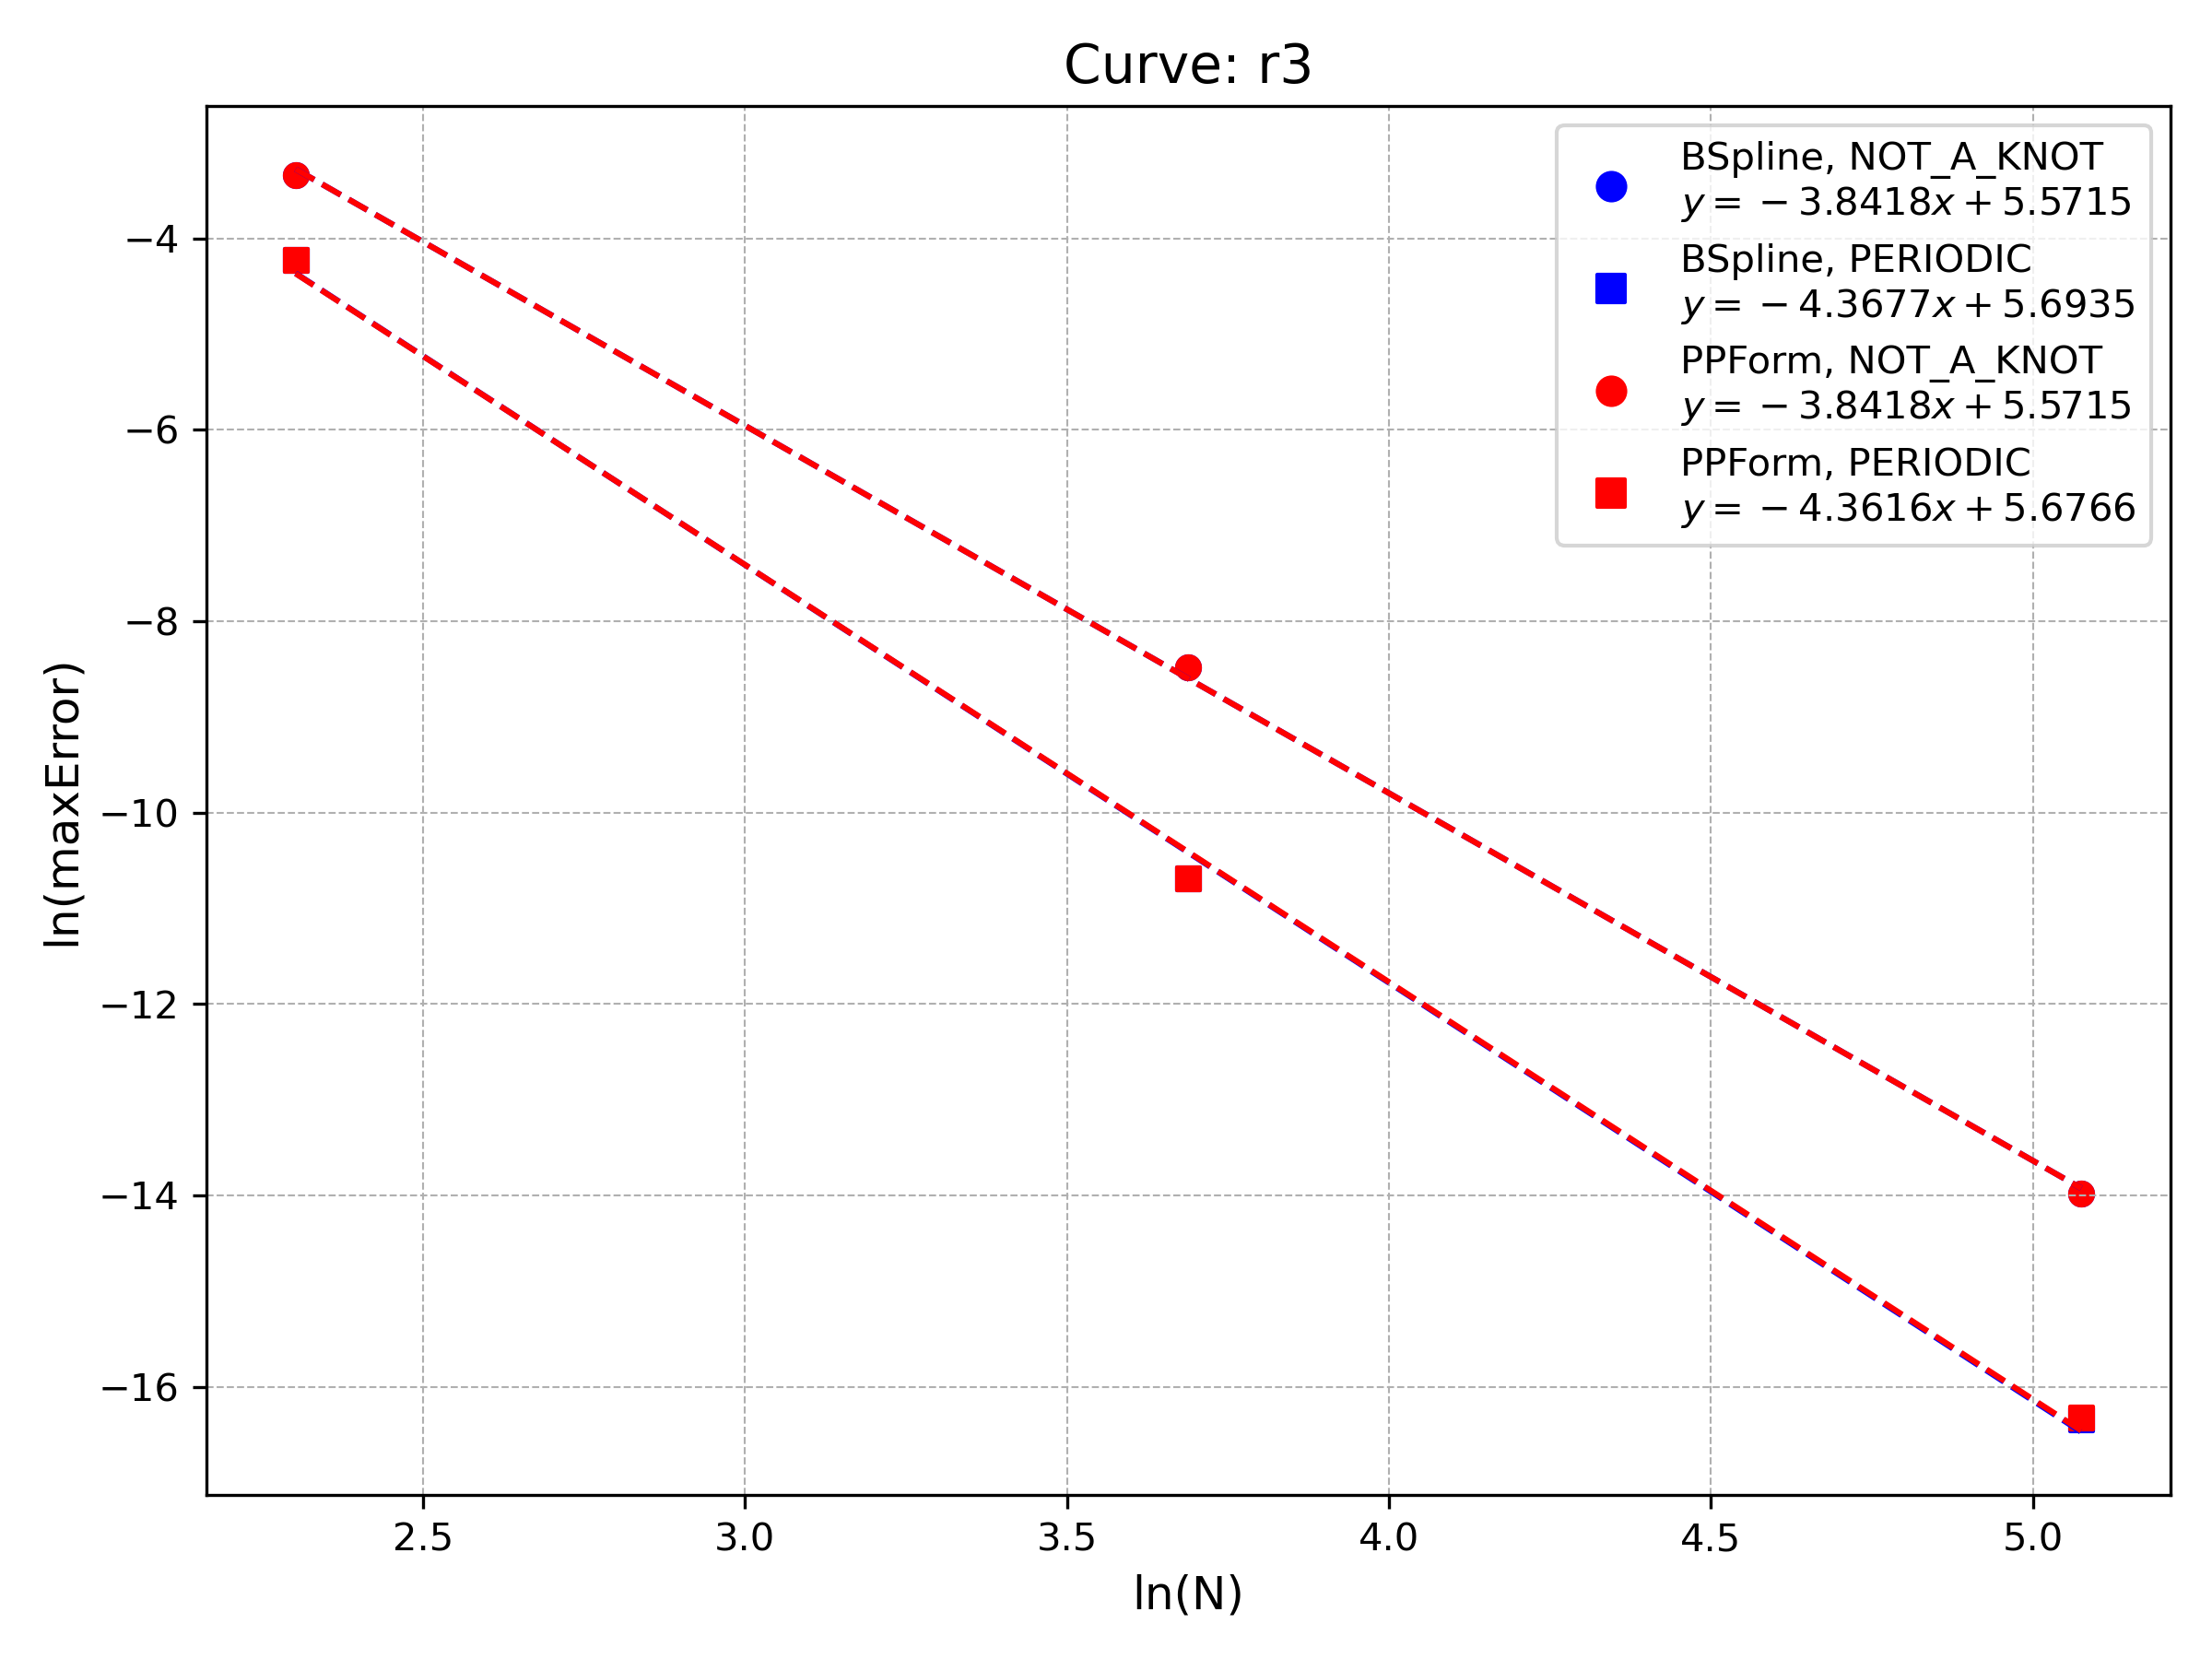
\includegraphics[width=0.45\textwidth]{../figure/problemE/r3_lnMaxError_vs_lnN.png}}
  \end{tabular}
  \renewcommand{\figurename}{Fig.}
  \caption{Least squares fit of the maximum errors of different curves under different methods with equidistant nodes}
  \label{fig:leastSquare_fit}
\end{figure}

It can be concluded that for the curve \(r_2\), the Complete boundary
condition, which provides the velocity information at both ends of the curve,
gives the best fitting effect, with the smallest error and the steepest slope.
For the curve \(r_1\), the Not-a-Knot boundary condition performs well in terms
of smoothness and accuracy. The Periodic boundary condition also provides a
similar effect to the Not-a-Knot boundary condition, ensuring smoothness and
continuity. For the curve \(r_3\), the periodic boundary condition provides the
best fitting effect. This is because the curve is inherently periodic, and
using periodic boundary conditions ensures that the curve is smooth and
continuous at the boundaries, avoiding any abrupt changes or discontinuities.

Special attention should be paid to the fitting of curve \(r_1\), as there are
two sharp extrema points, resulting in larger errors near these points. In
practical curve fitting, segmented fitting around these points can be used to
improve the fitting effect.

The max errors analysis of different boundary conditions for B-spline
interpolation reveals the following insights:

\textbf{Clamped or Complete Boundary}
\begin{itemize}
  \item \textbf{Suitable for:} Scenarios where boundary derivatives (e.g., slope or velocity) are known, such as when the slope of the interpolating curve is determined by physical conditions.
  \item \textbf{Advantages:} Allows precise control over boundary behavior, suitable for well-constrained situations.
  \item \textbf{Disadvantages:} If the specified derivative values are inaccurate, the overall interpolation quality may degrade.
\end{itemize}

\textbf{Second Derivative Boundary}
\begin{itemize}
  \item \textbf{Suitable for:} Scenarios where boundary curvature is known, such as in certain mechanical modeling applications.
  \item \textbf{Advantages:} Suitable for scenarios sensitive to boundary curvature, allowing more accurate simulation of boundary behavior.
  \item \textbf{Disadvantages:} Requires accurate second derivative values.
\end{itemize}

\textbf{Not-a-Knot Boundary}
\begin{itemize}
  \item \textbf{Suitable for:} Data without distinct boundary features, requiring higher-order continuity without imposing excessive constraints.
  \item \textbf{Advantages:} Produces curves with better global continuity, automatically smoothing the curve.
  \item \textbf{Disadvantages:} Boundary behavior may not always meet expectations.
\end{itemize}

\textbf{Periodic Boundary:}
\begin{itemize}
  \item \textbf{Suitable for:} Inherently periodic data, such as 24-hour temperature distributions in time series.
  \item \textbf{Advantages:} Naturally closed curves without abrupt boundary behavior.
  \item \textbf{Disadvantages:} Forcing non-periodic data into a periodic boundary may result in unnatural fitting.
\end{itemize}

This explains why, in the above curve fitting, different boundary conditions
can be theoretically selected based on the nature of the curve and initial
conditions to achieve the best fitting effect.

Finally, I will show the B-spline fitting curves of the three curves under the
best boundary conditions with different data points, to compare and analyze the
fitting effects of cumulative chordal length and equidistant nodes.

\begin{figure}[H]
  \centering
  \begin{tabular}{cc}
    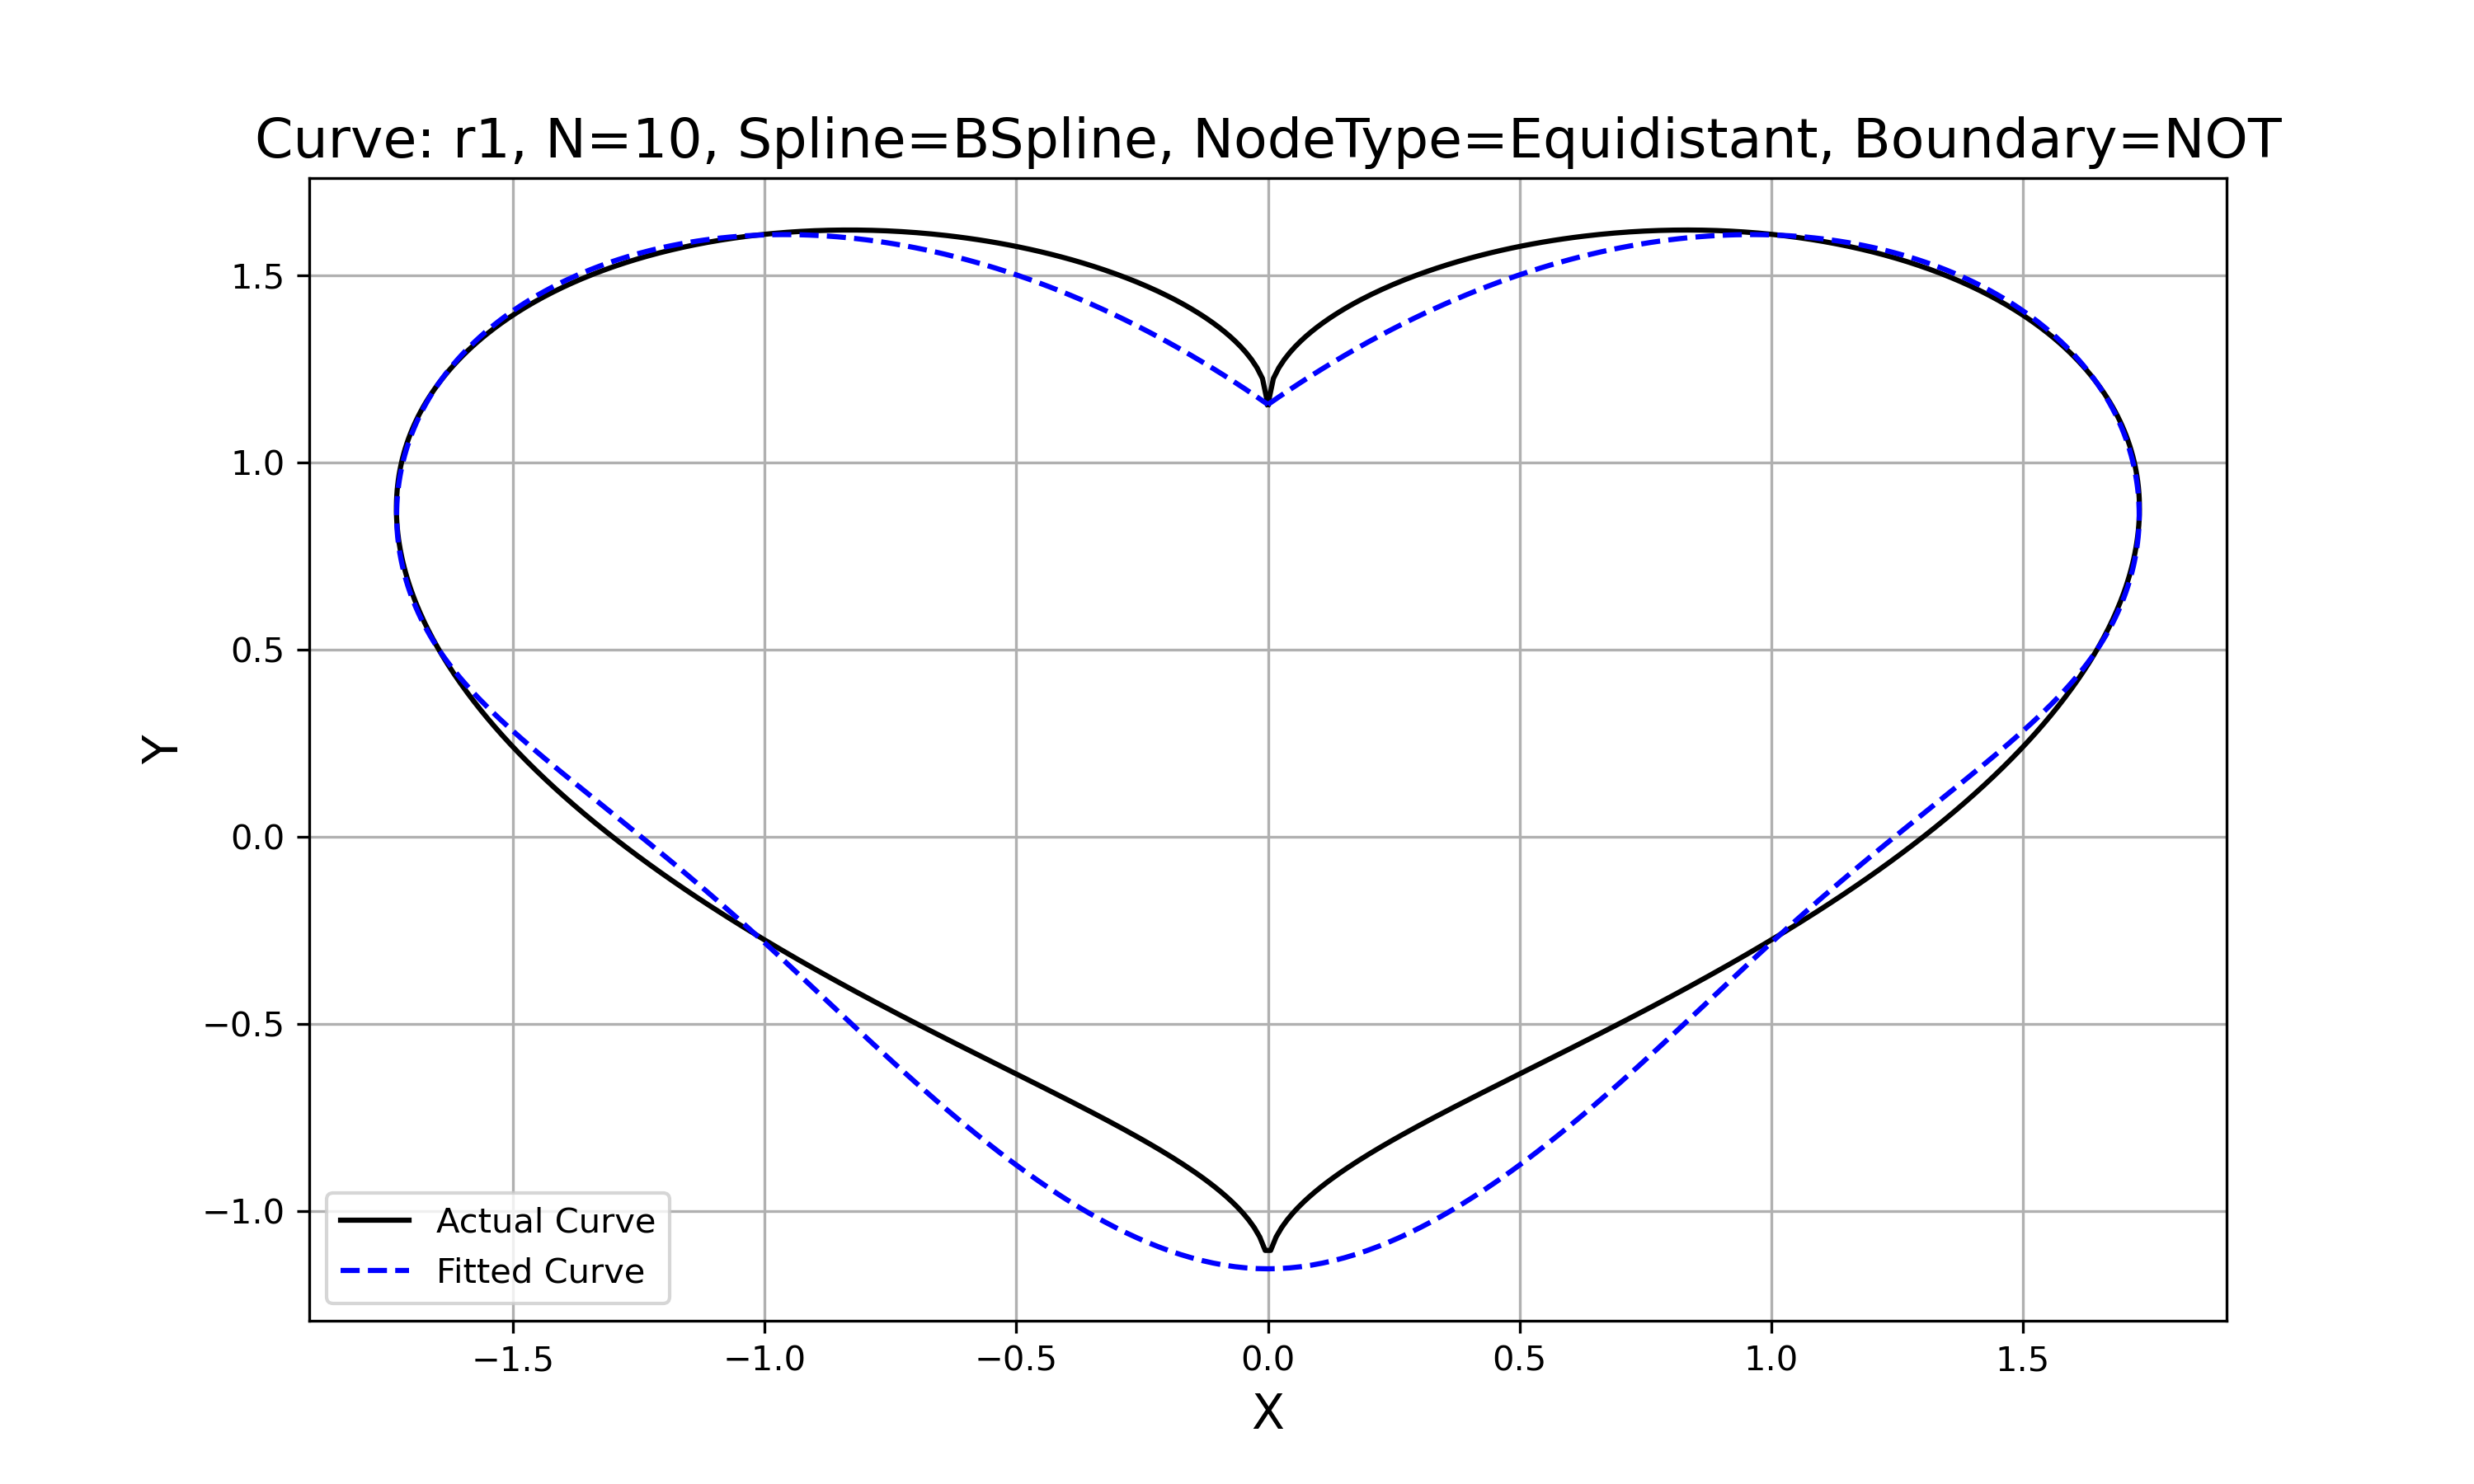
\includegraphics[width=0.45\textwidth]{../figure/problemE/N_10_r1_BSpline_Equidistant_NOT.png}  &
    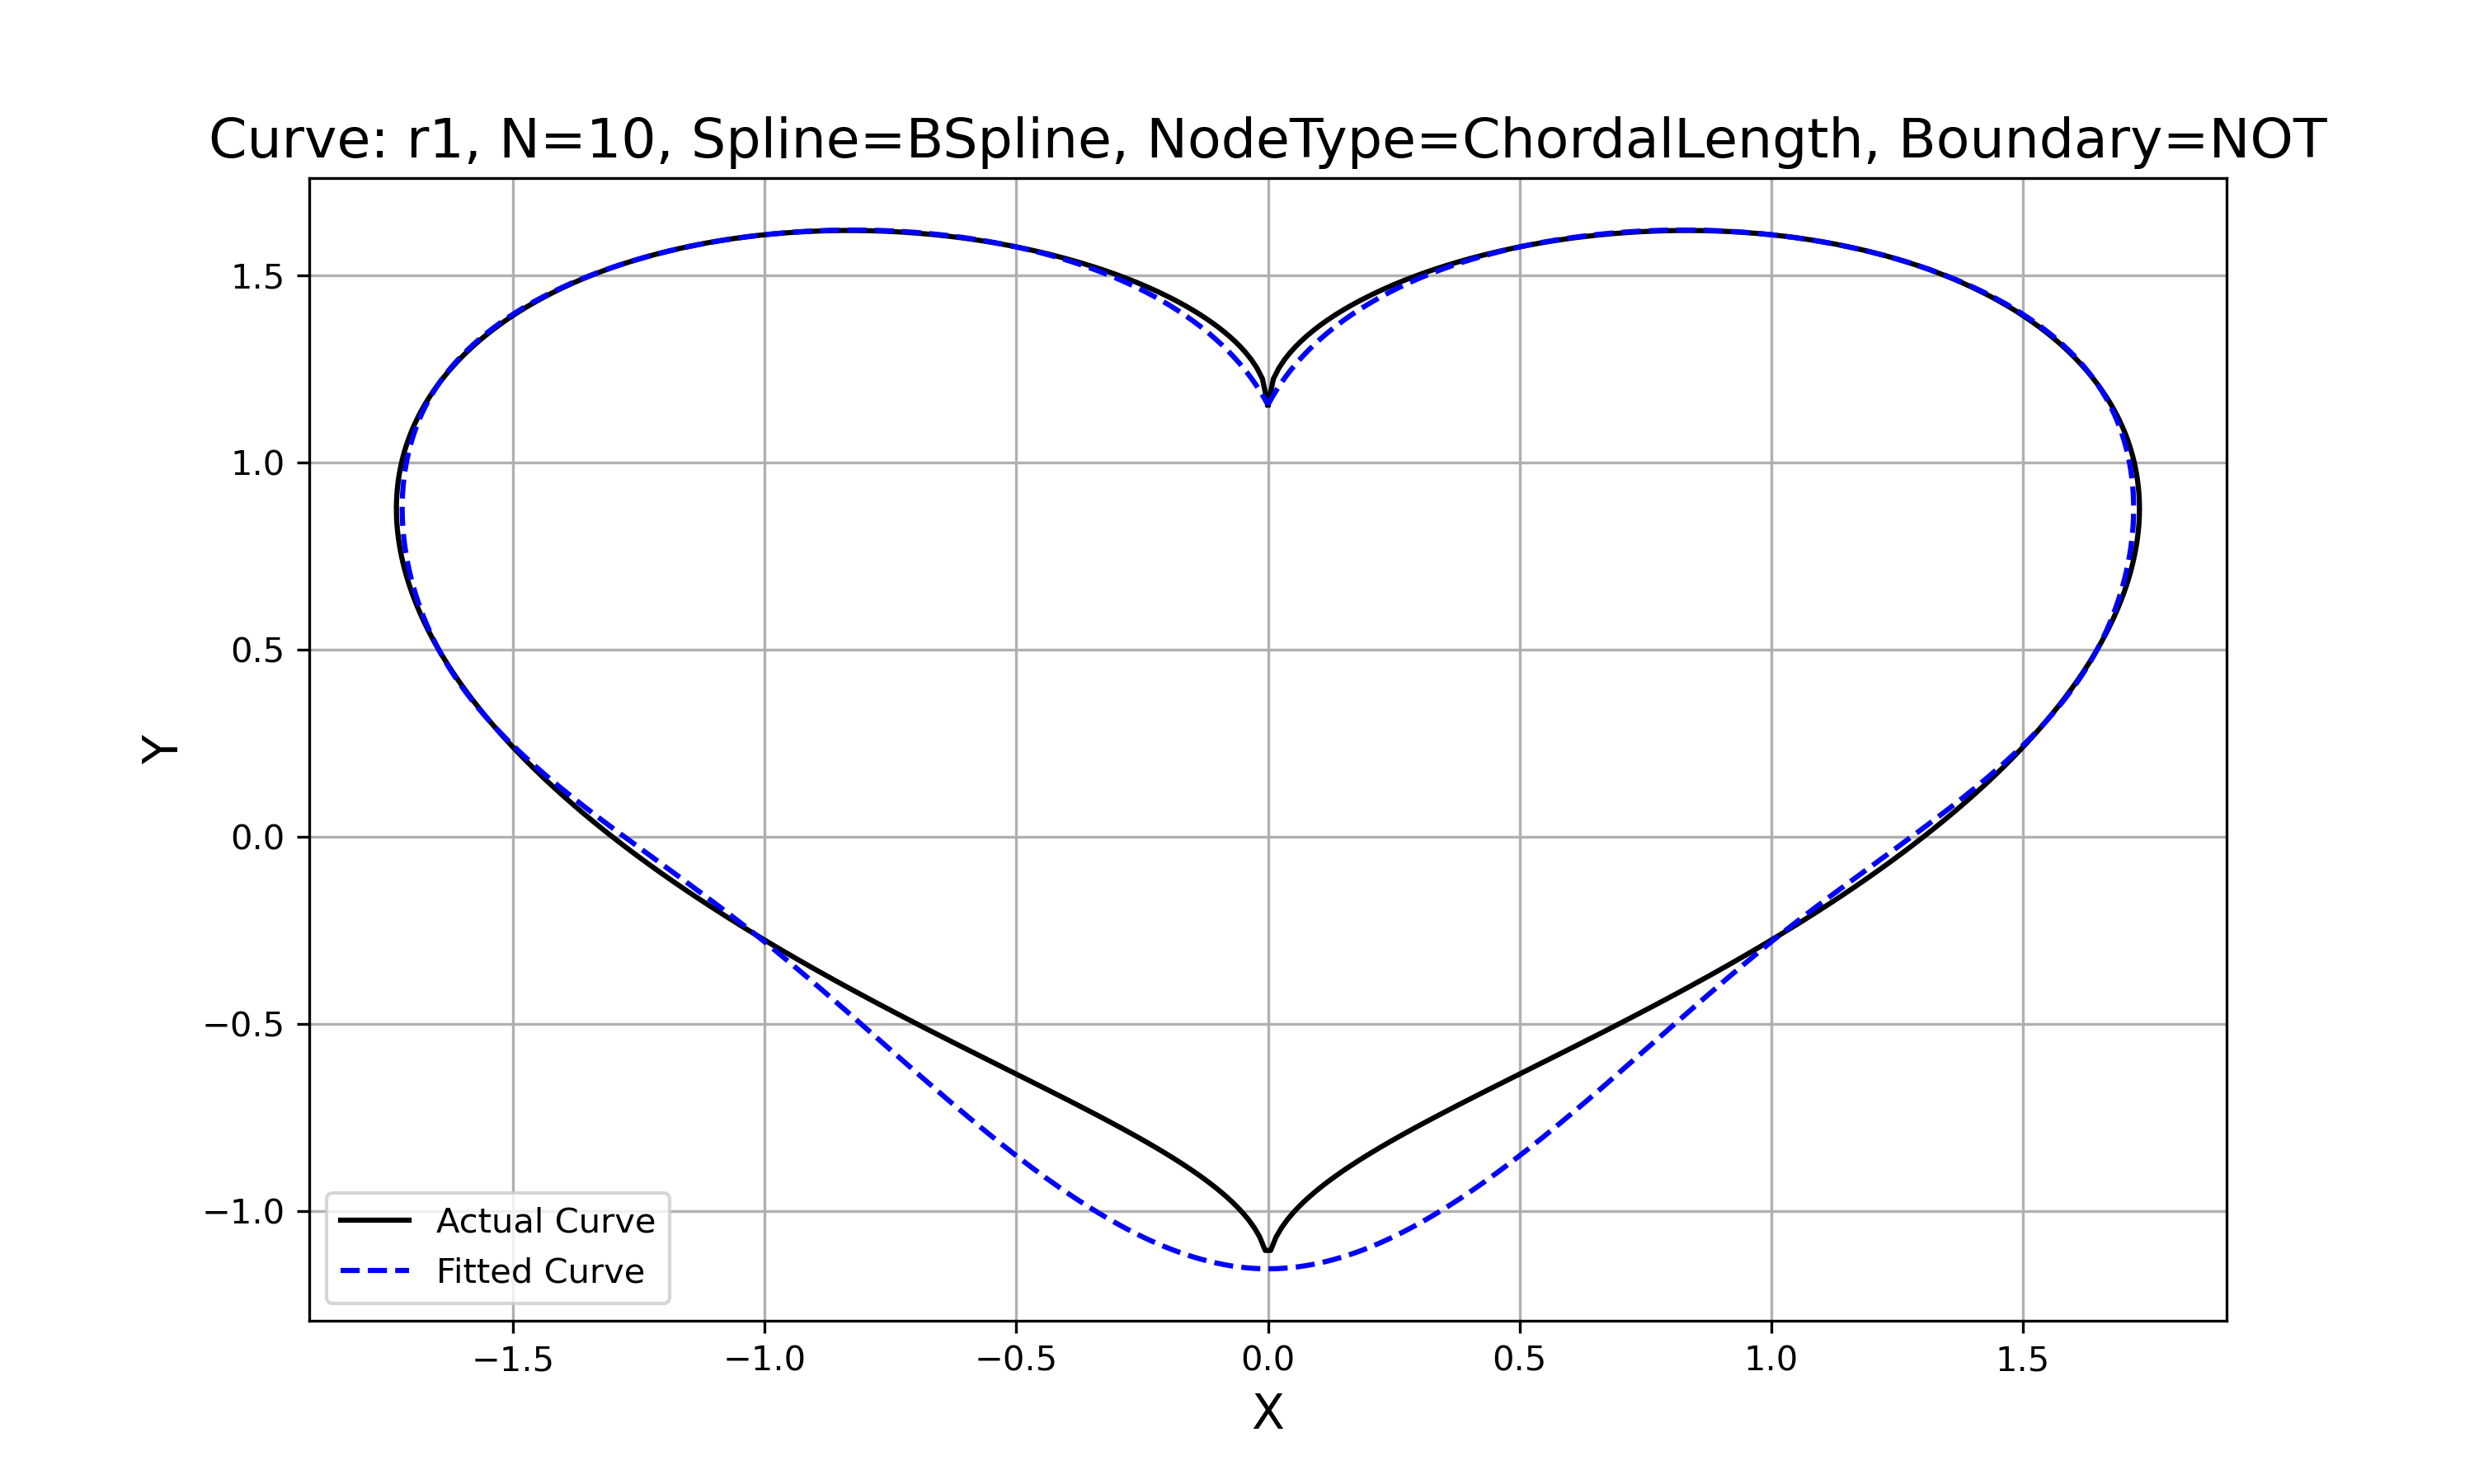
\includegraphics[width=0.45\textwidth]{../figure/problemE/N_10_r1_BSpline_ChordalLength_NOT.png}  \\
    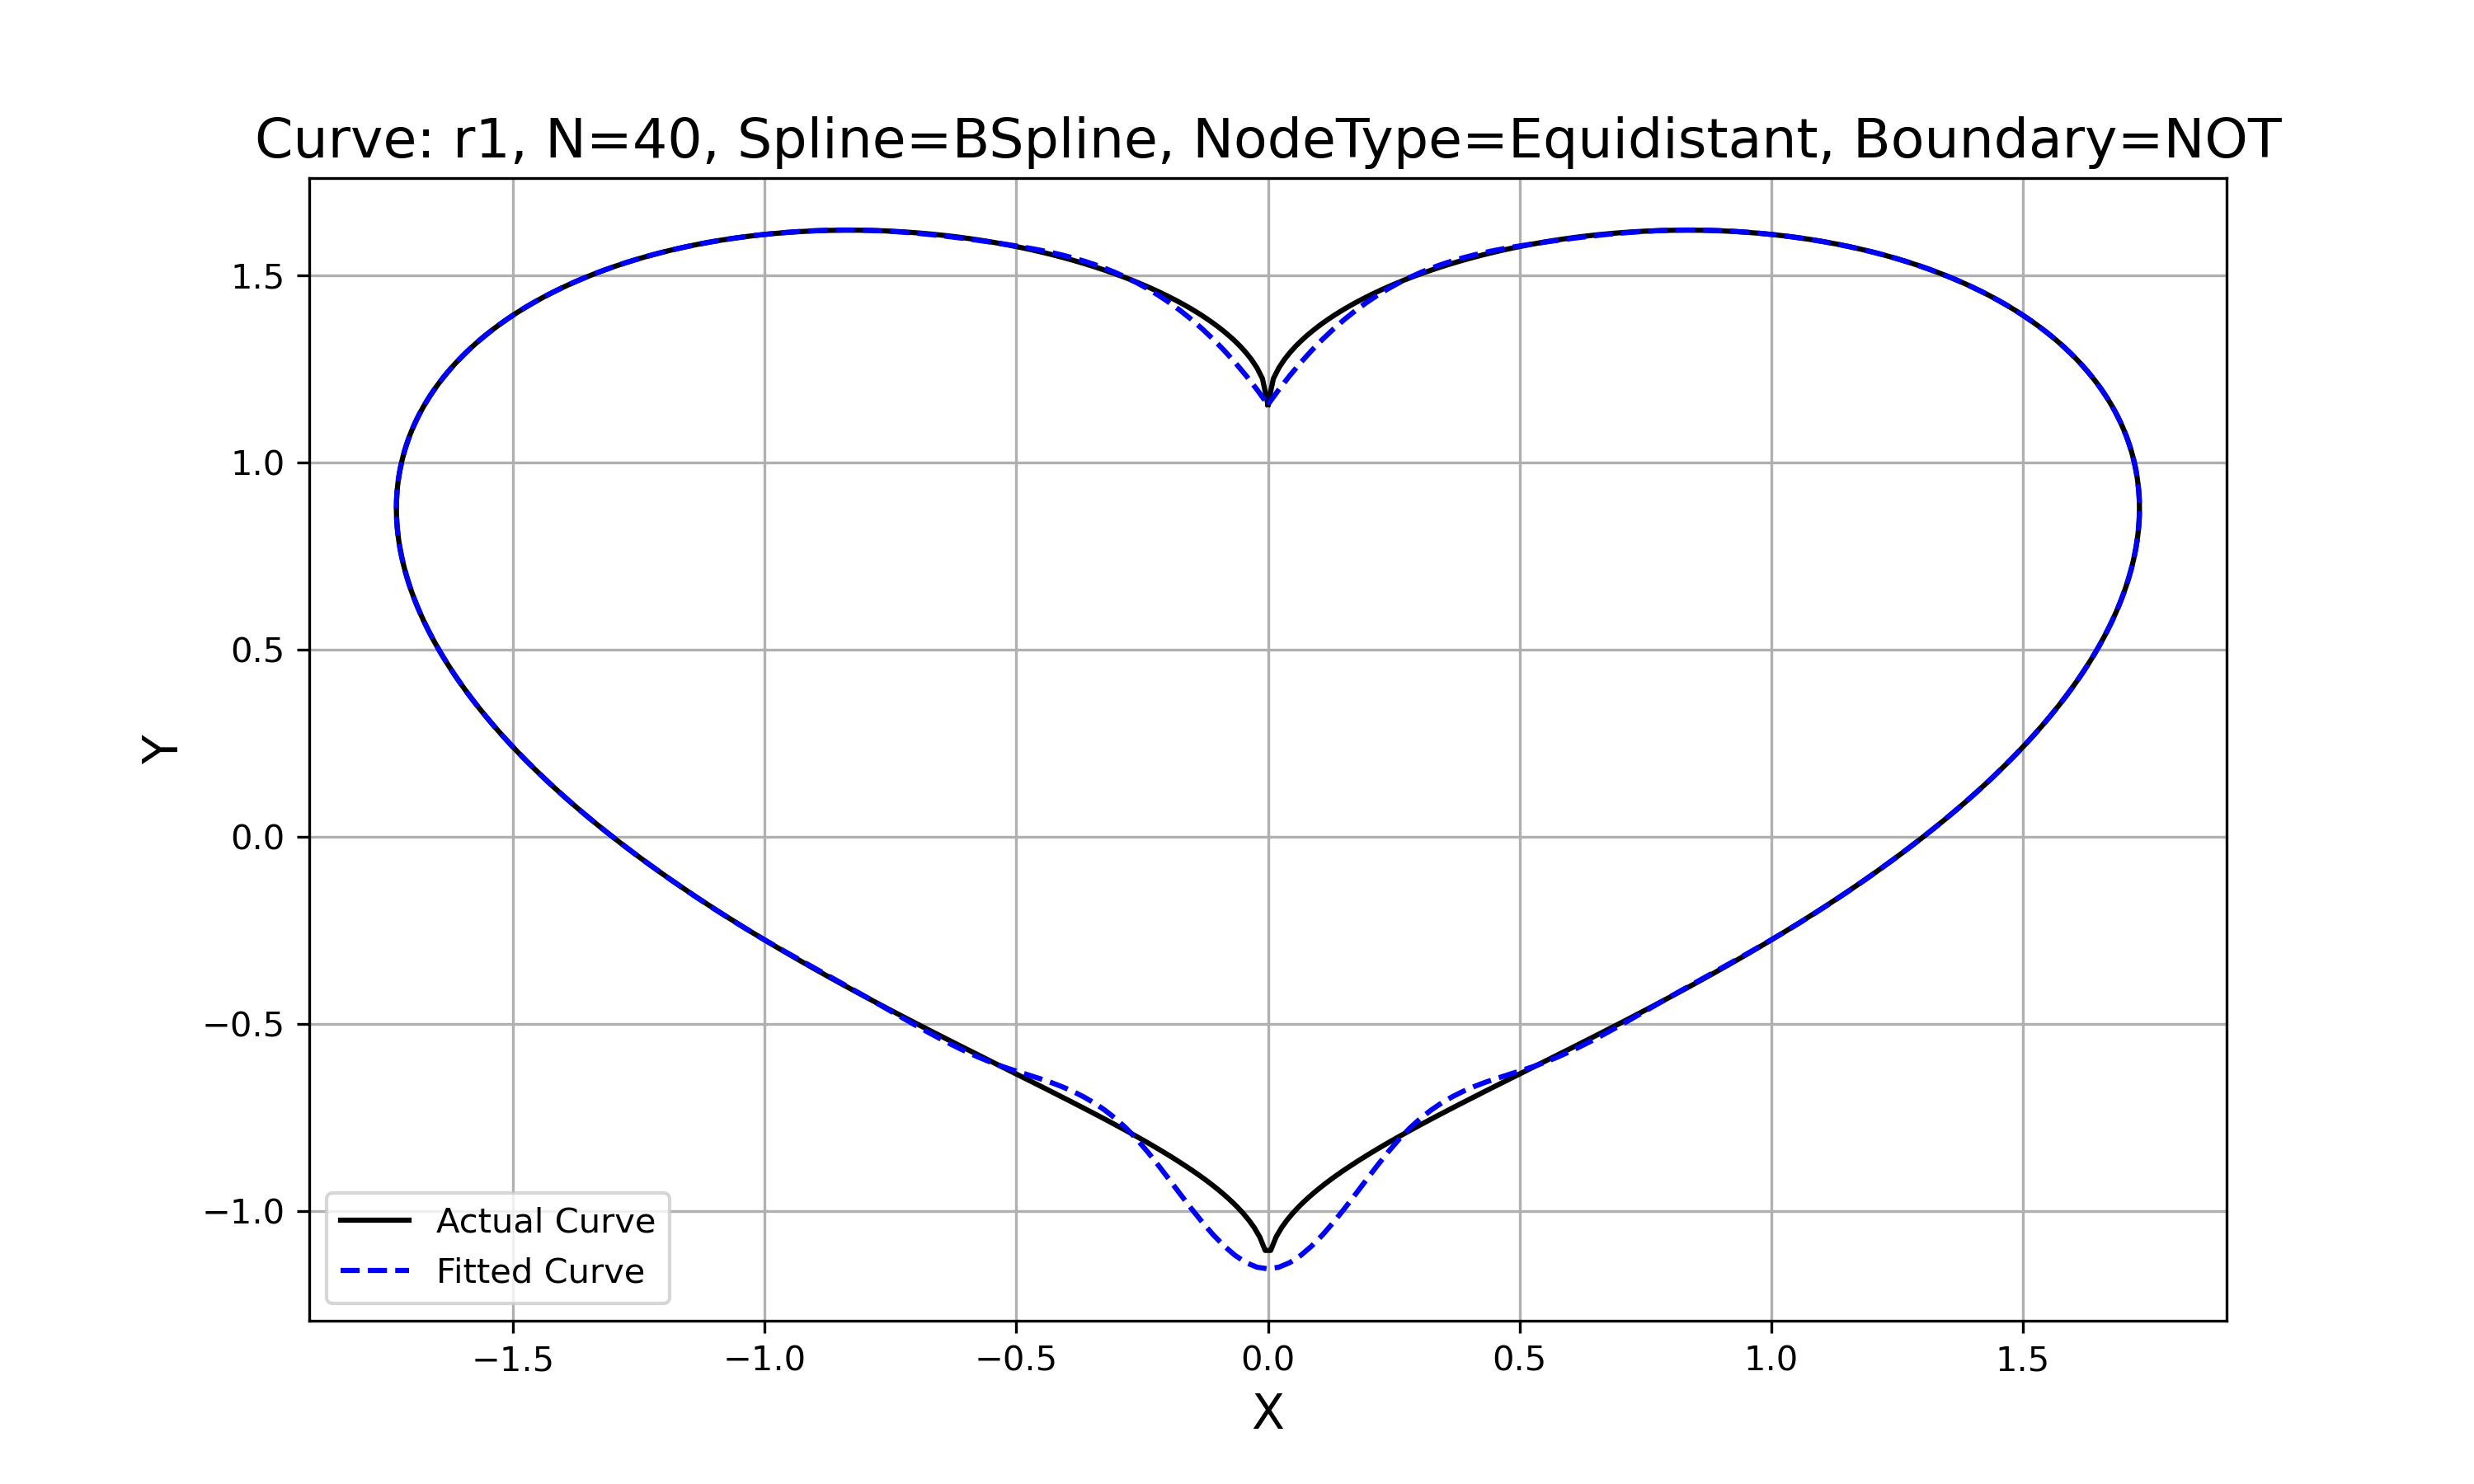
\includegraphics[width=0.45\textwidth]{../figure/problemE/N_40_r1_BSpline_Equidistant_NOT.png}  &
    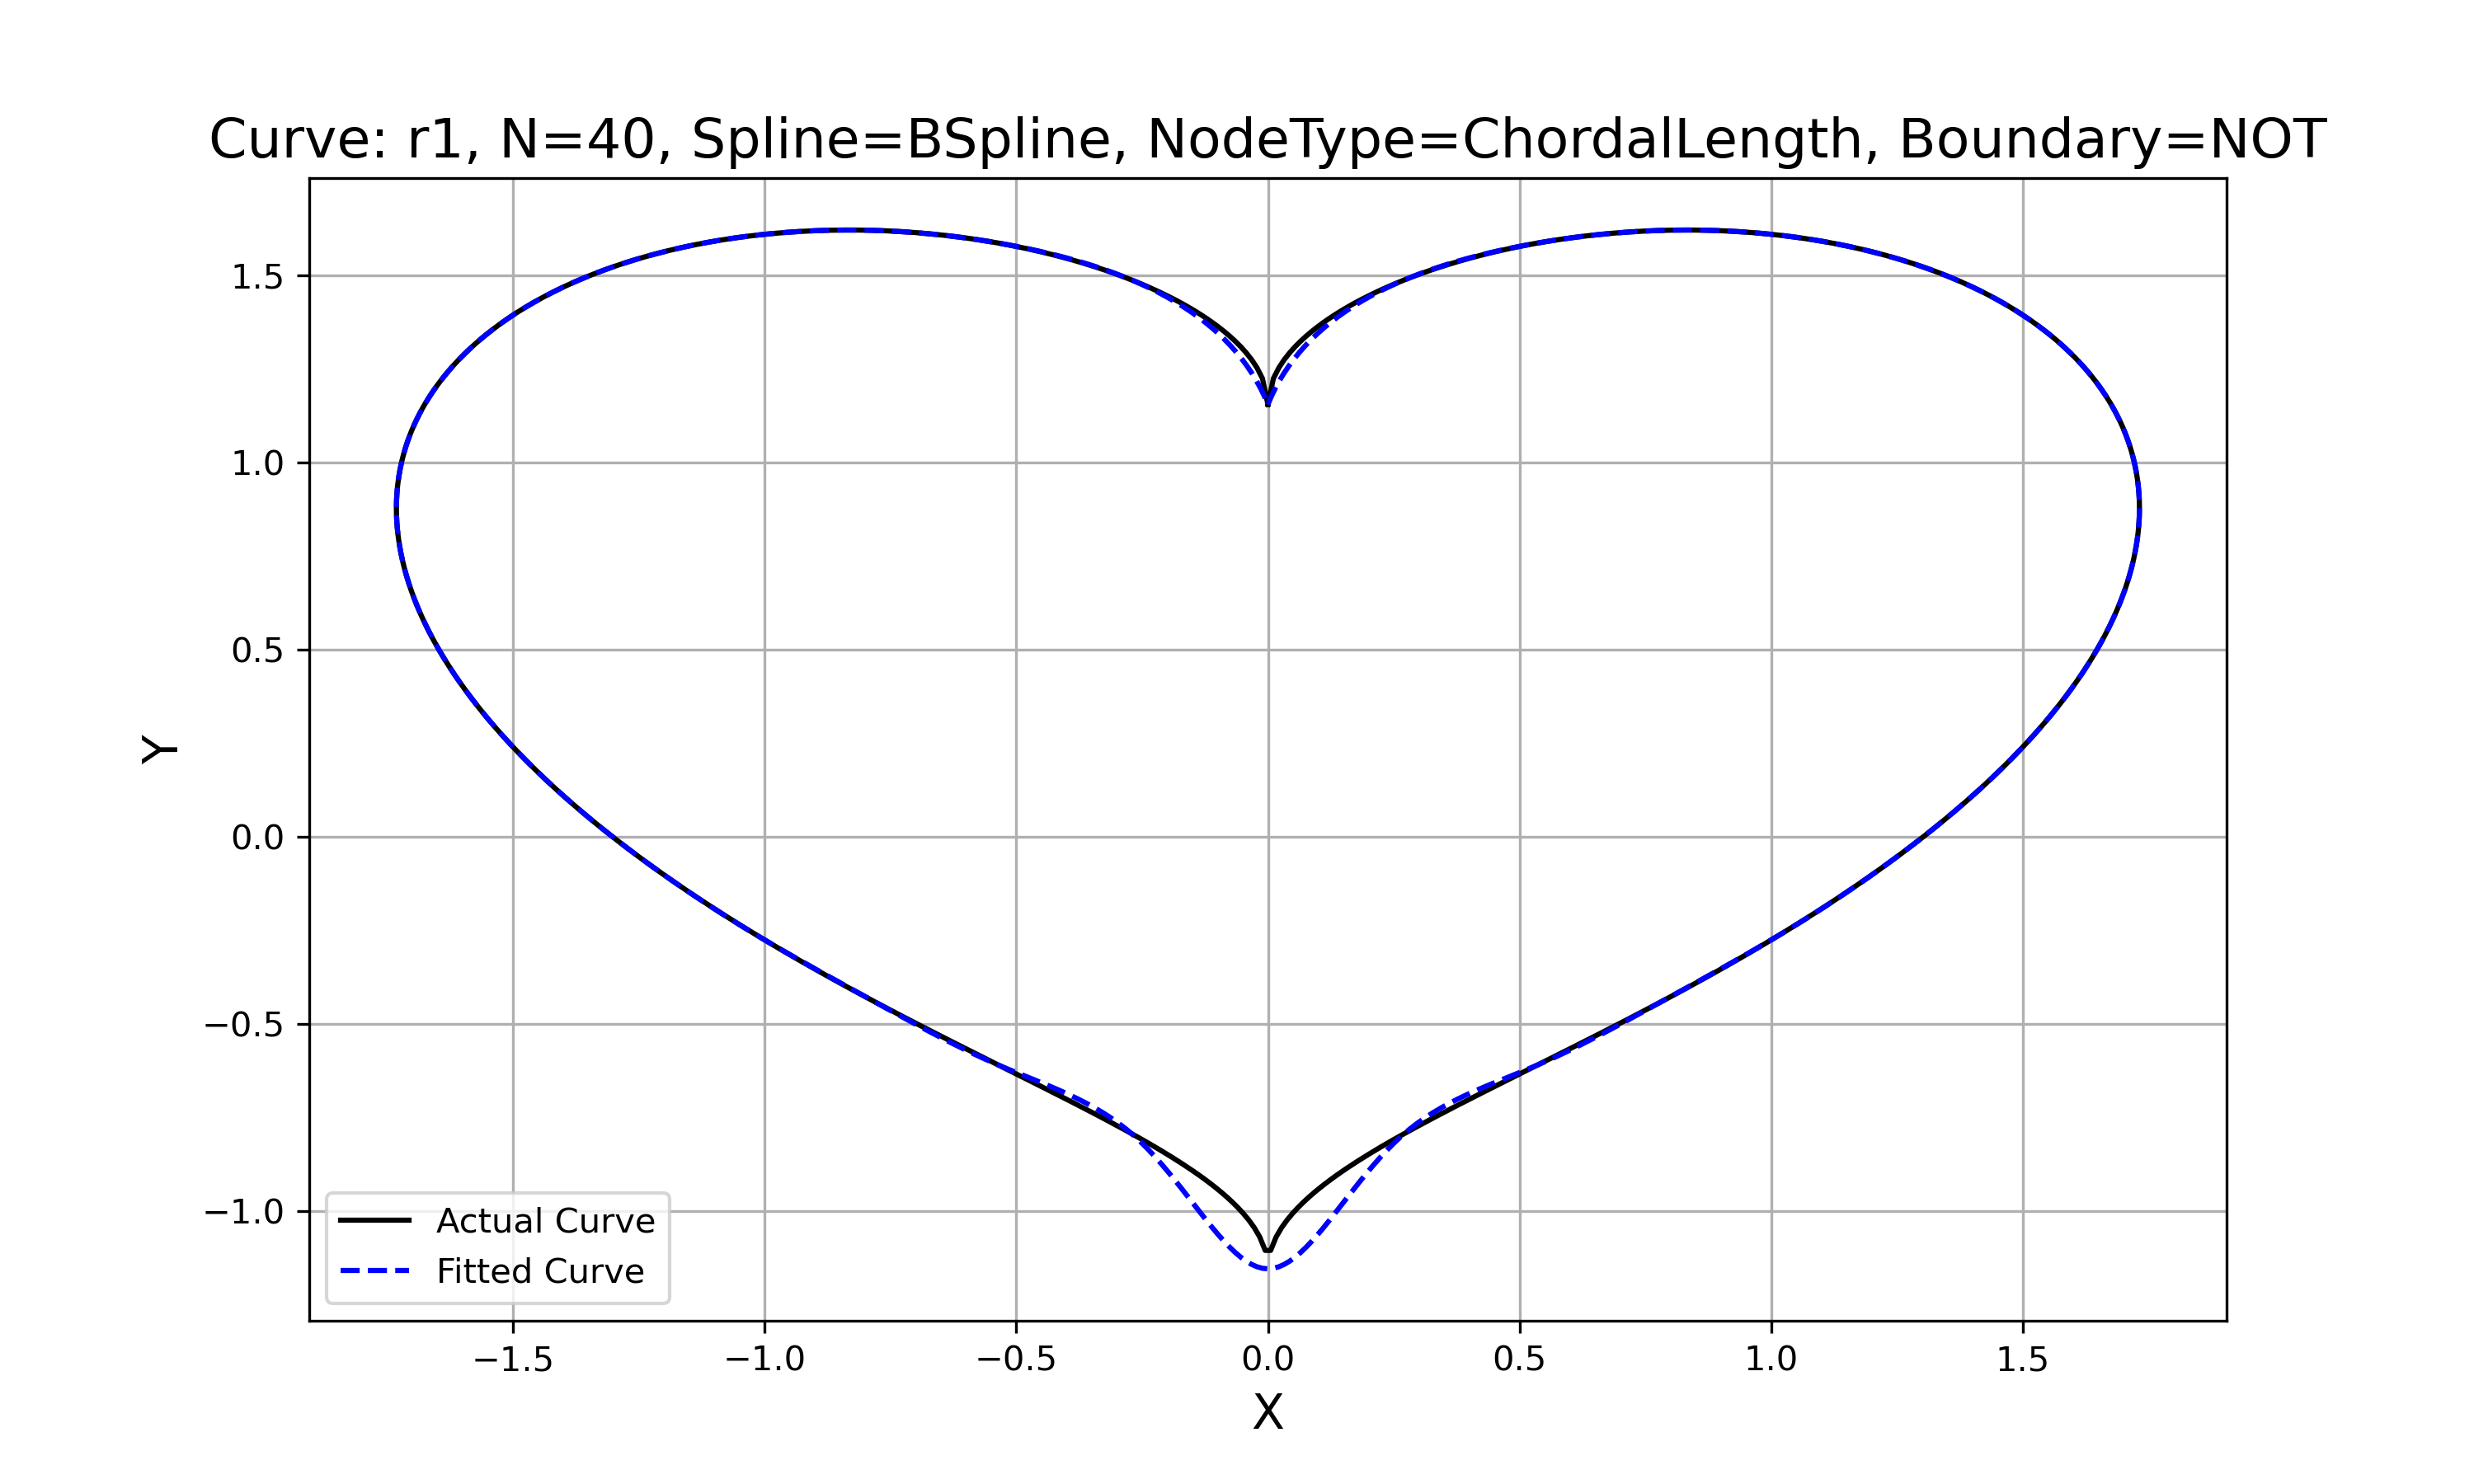
\includegraphics[width=0.45\textwidth]{../figure/problemE/N_40_r1_BSpline_ChordalLength_NOT.png}  \\
    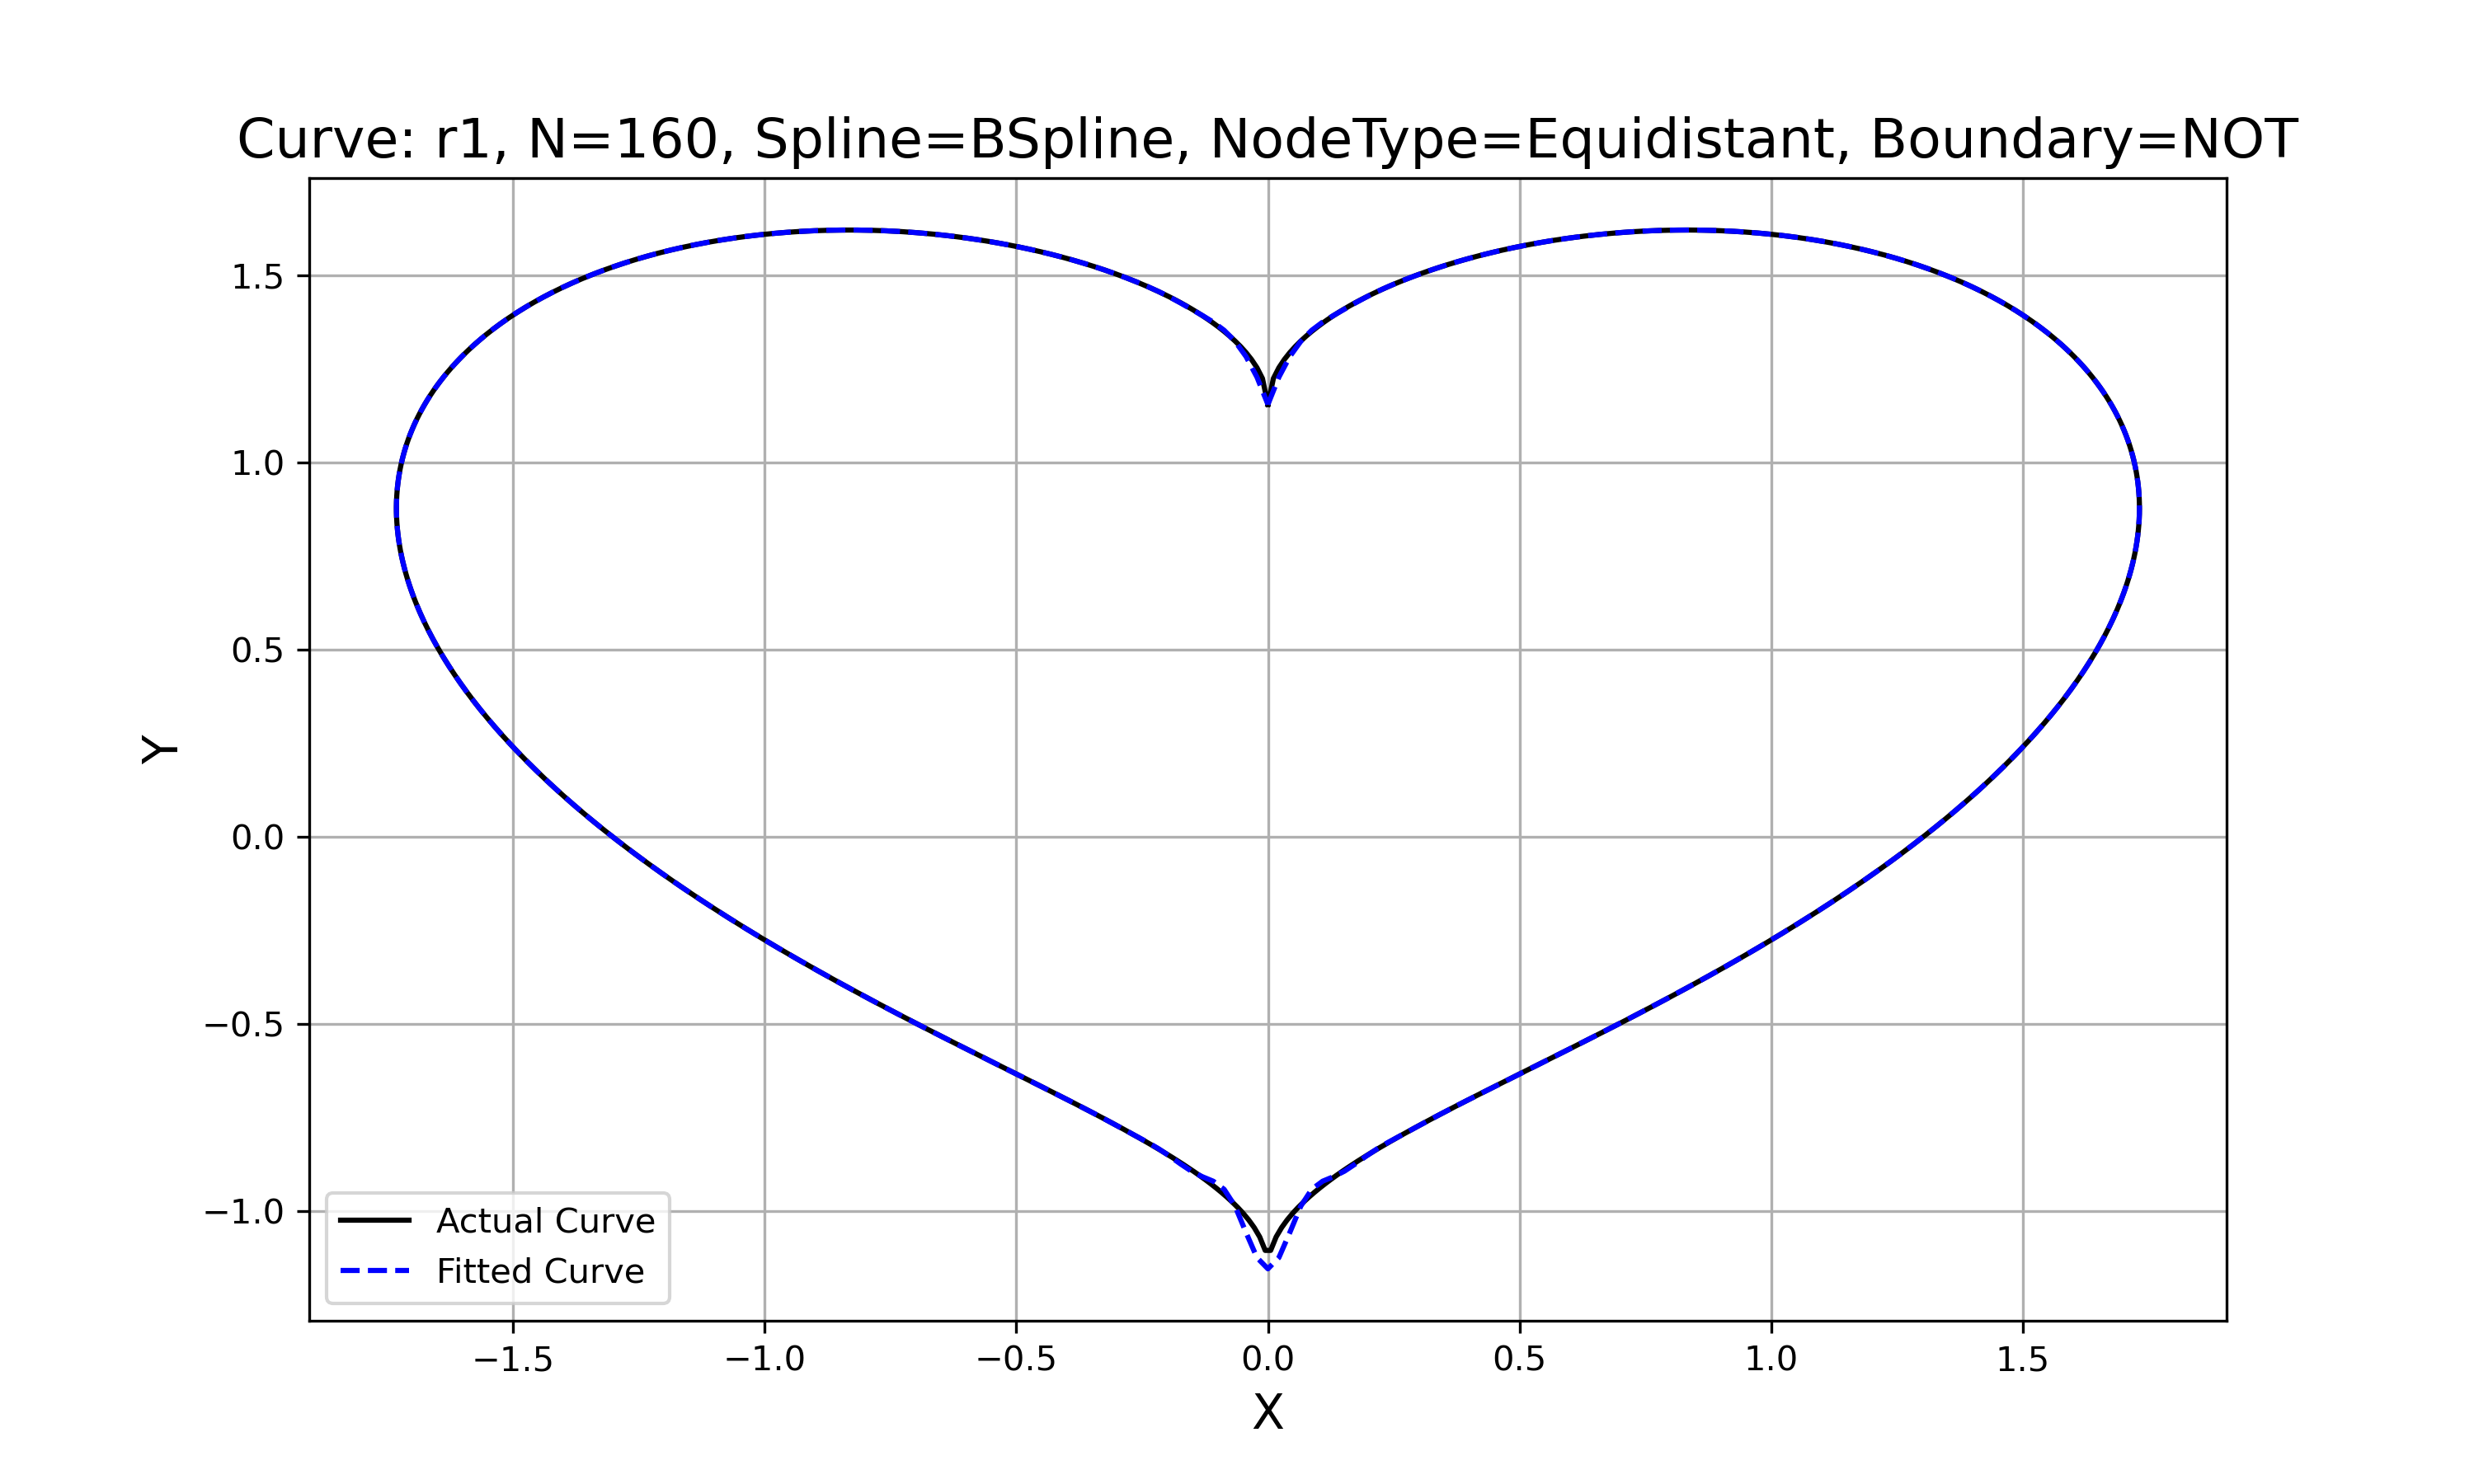
\includegraphics[width=0.45\textwidth]{../figure/problemE/N_160_r1_BSpline_Equidistant_NOT.png} &
    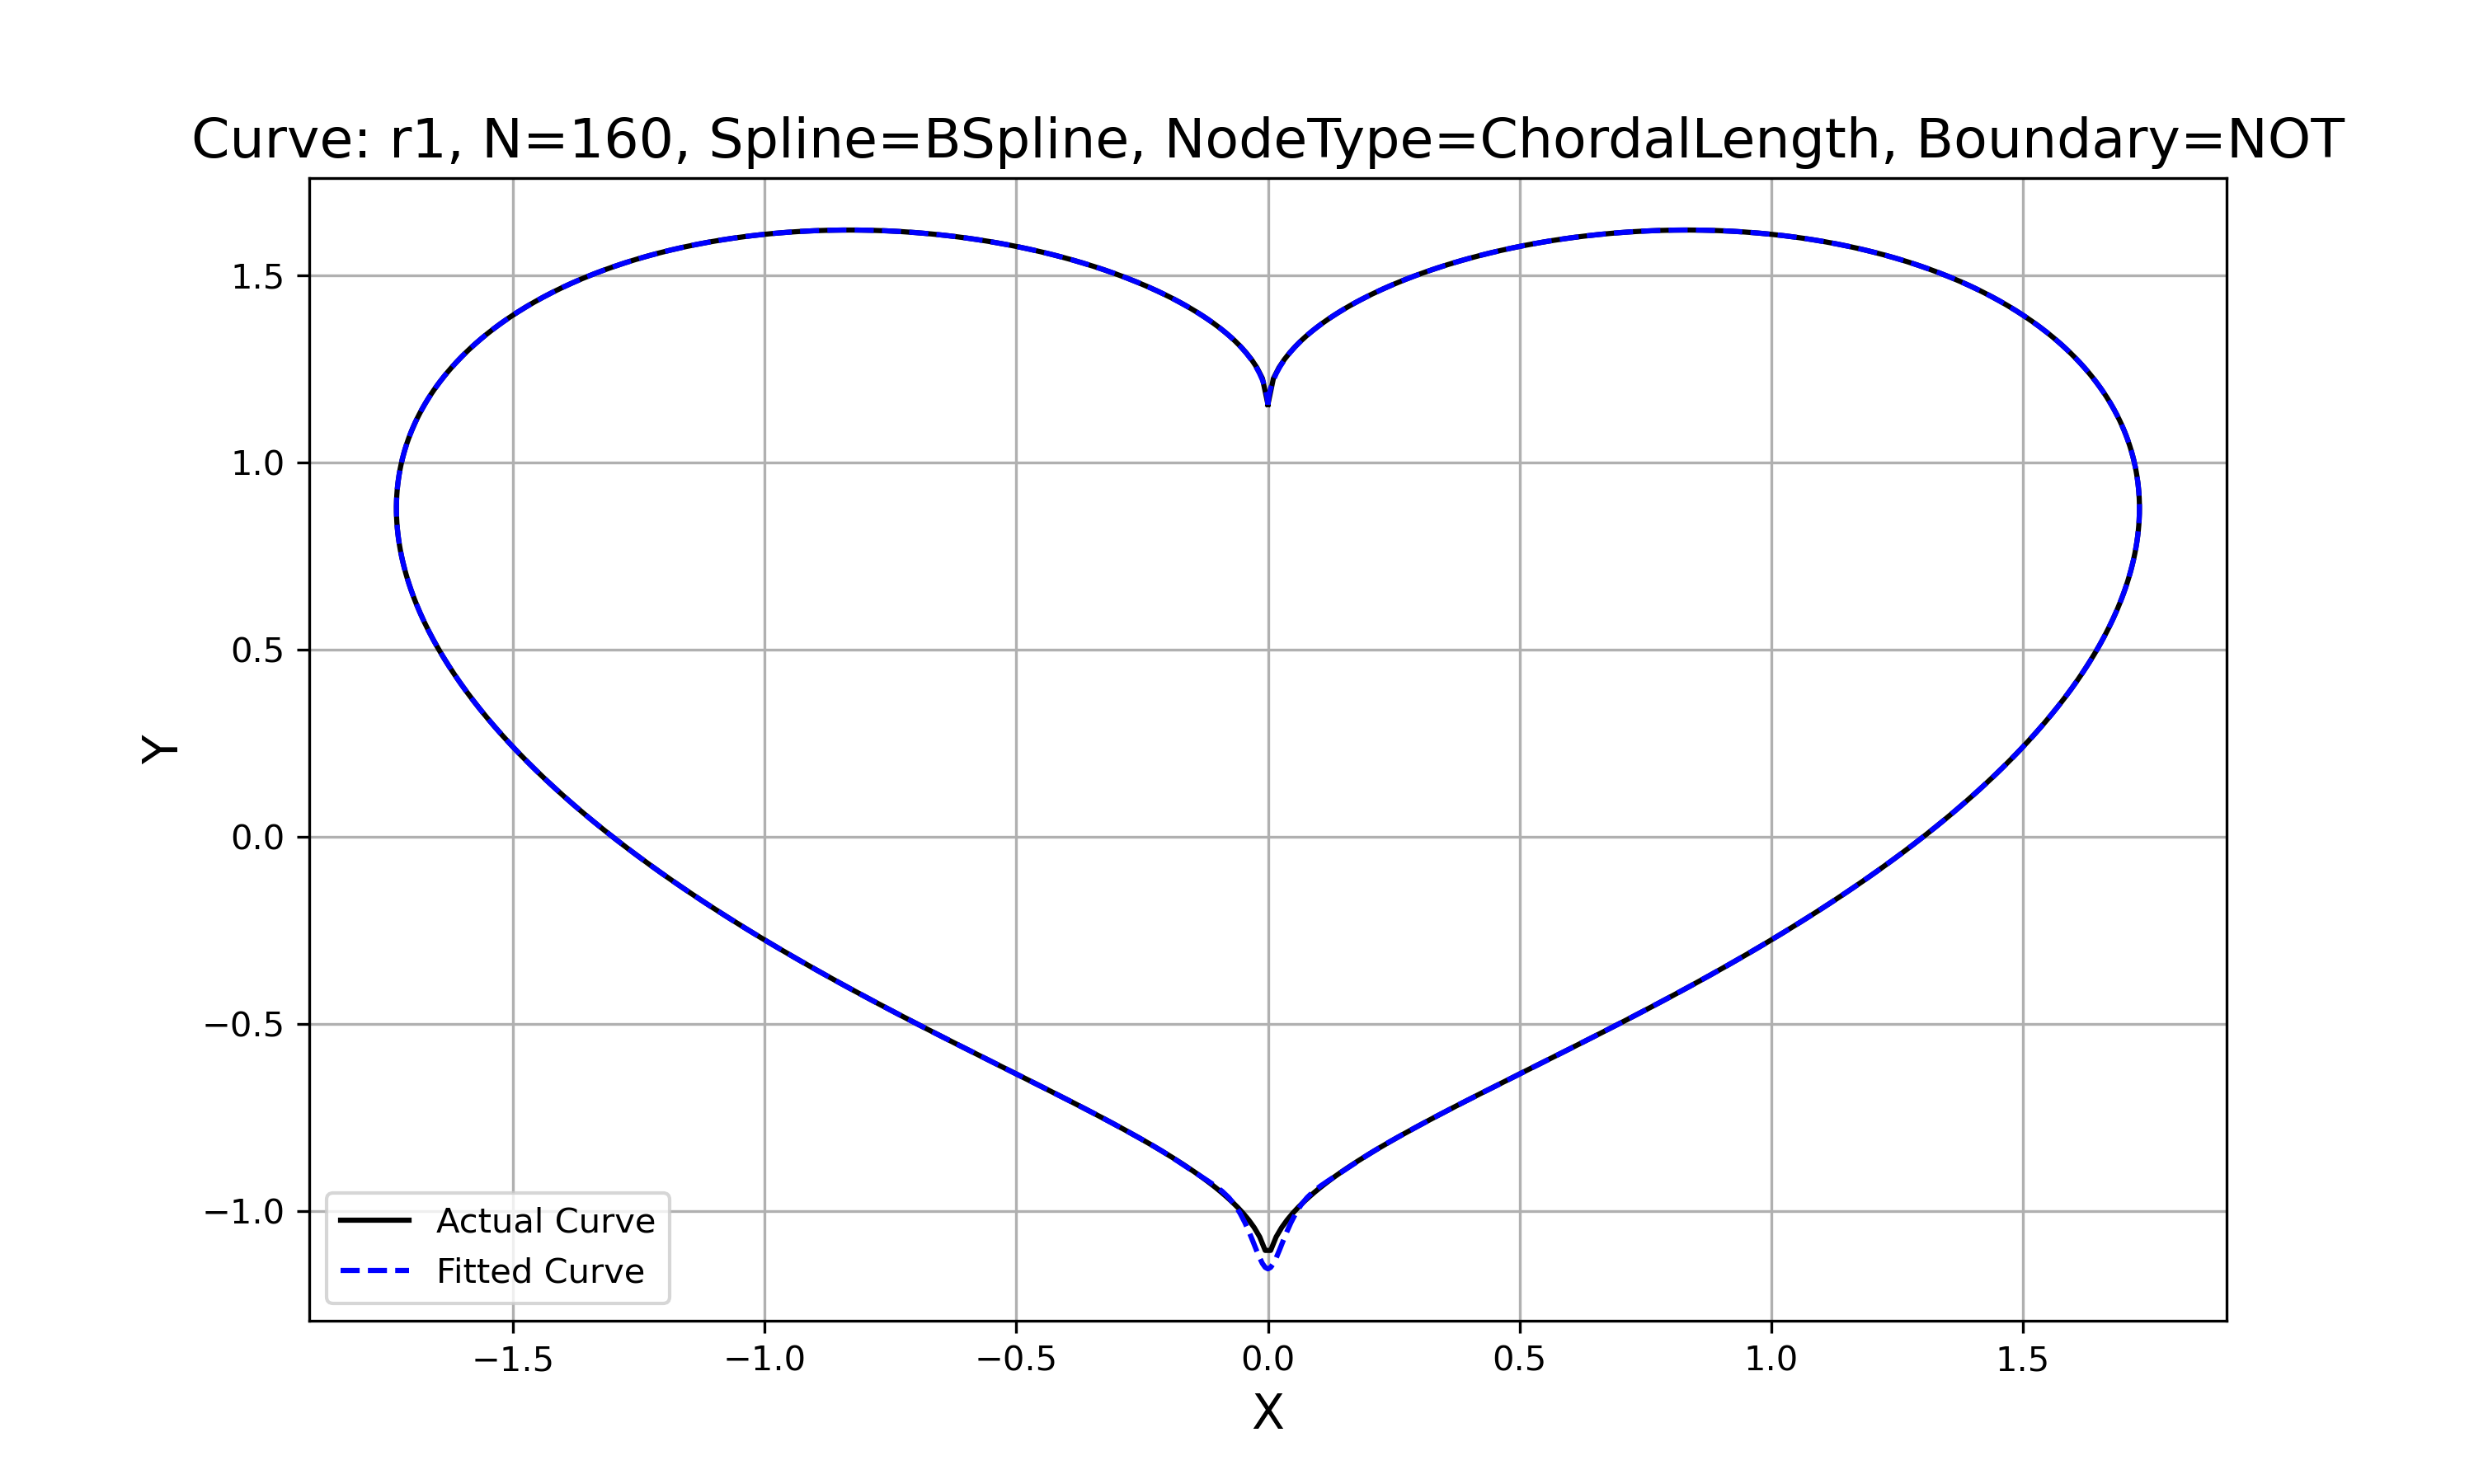
\includegraphics[width=0.45\textwidth]{../figure/problemE/N_160_r1_BSpline_ChordalLength_NOT.png} \\
  \end{tabular}
  \renewcommand{\figurename}{Fig.}
  \caption{Comparison of Equidistant and Chordal Length for curve \(r_1\) with NOT boundary condition}
  \label{fig:r1_nodeType_compare}
\end{figure}

The fitting effect of curve \(r_1\) is shown in
Fig.\ref{fig:r1_nodeType_compare}. The left column is for equidistant nodes,
and the right column is for cumulative chordal length. Each row corresponds to
a different number of data points. It can be seen that the cumulative chordal
length method performs better in areas with sharp changes, such as the tip of
the heart, while the equidistant nodes perform better in smoother areas.

\begin{figure}[H]
  \centering
  \begin{tabular}{cc}
    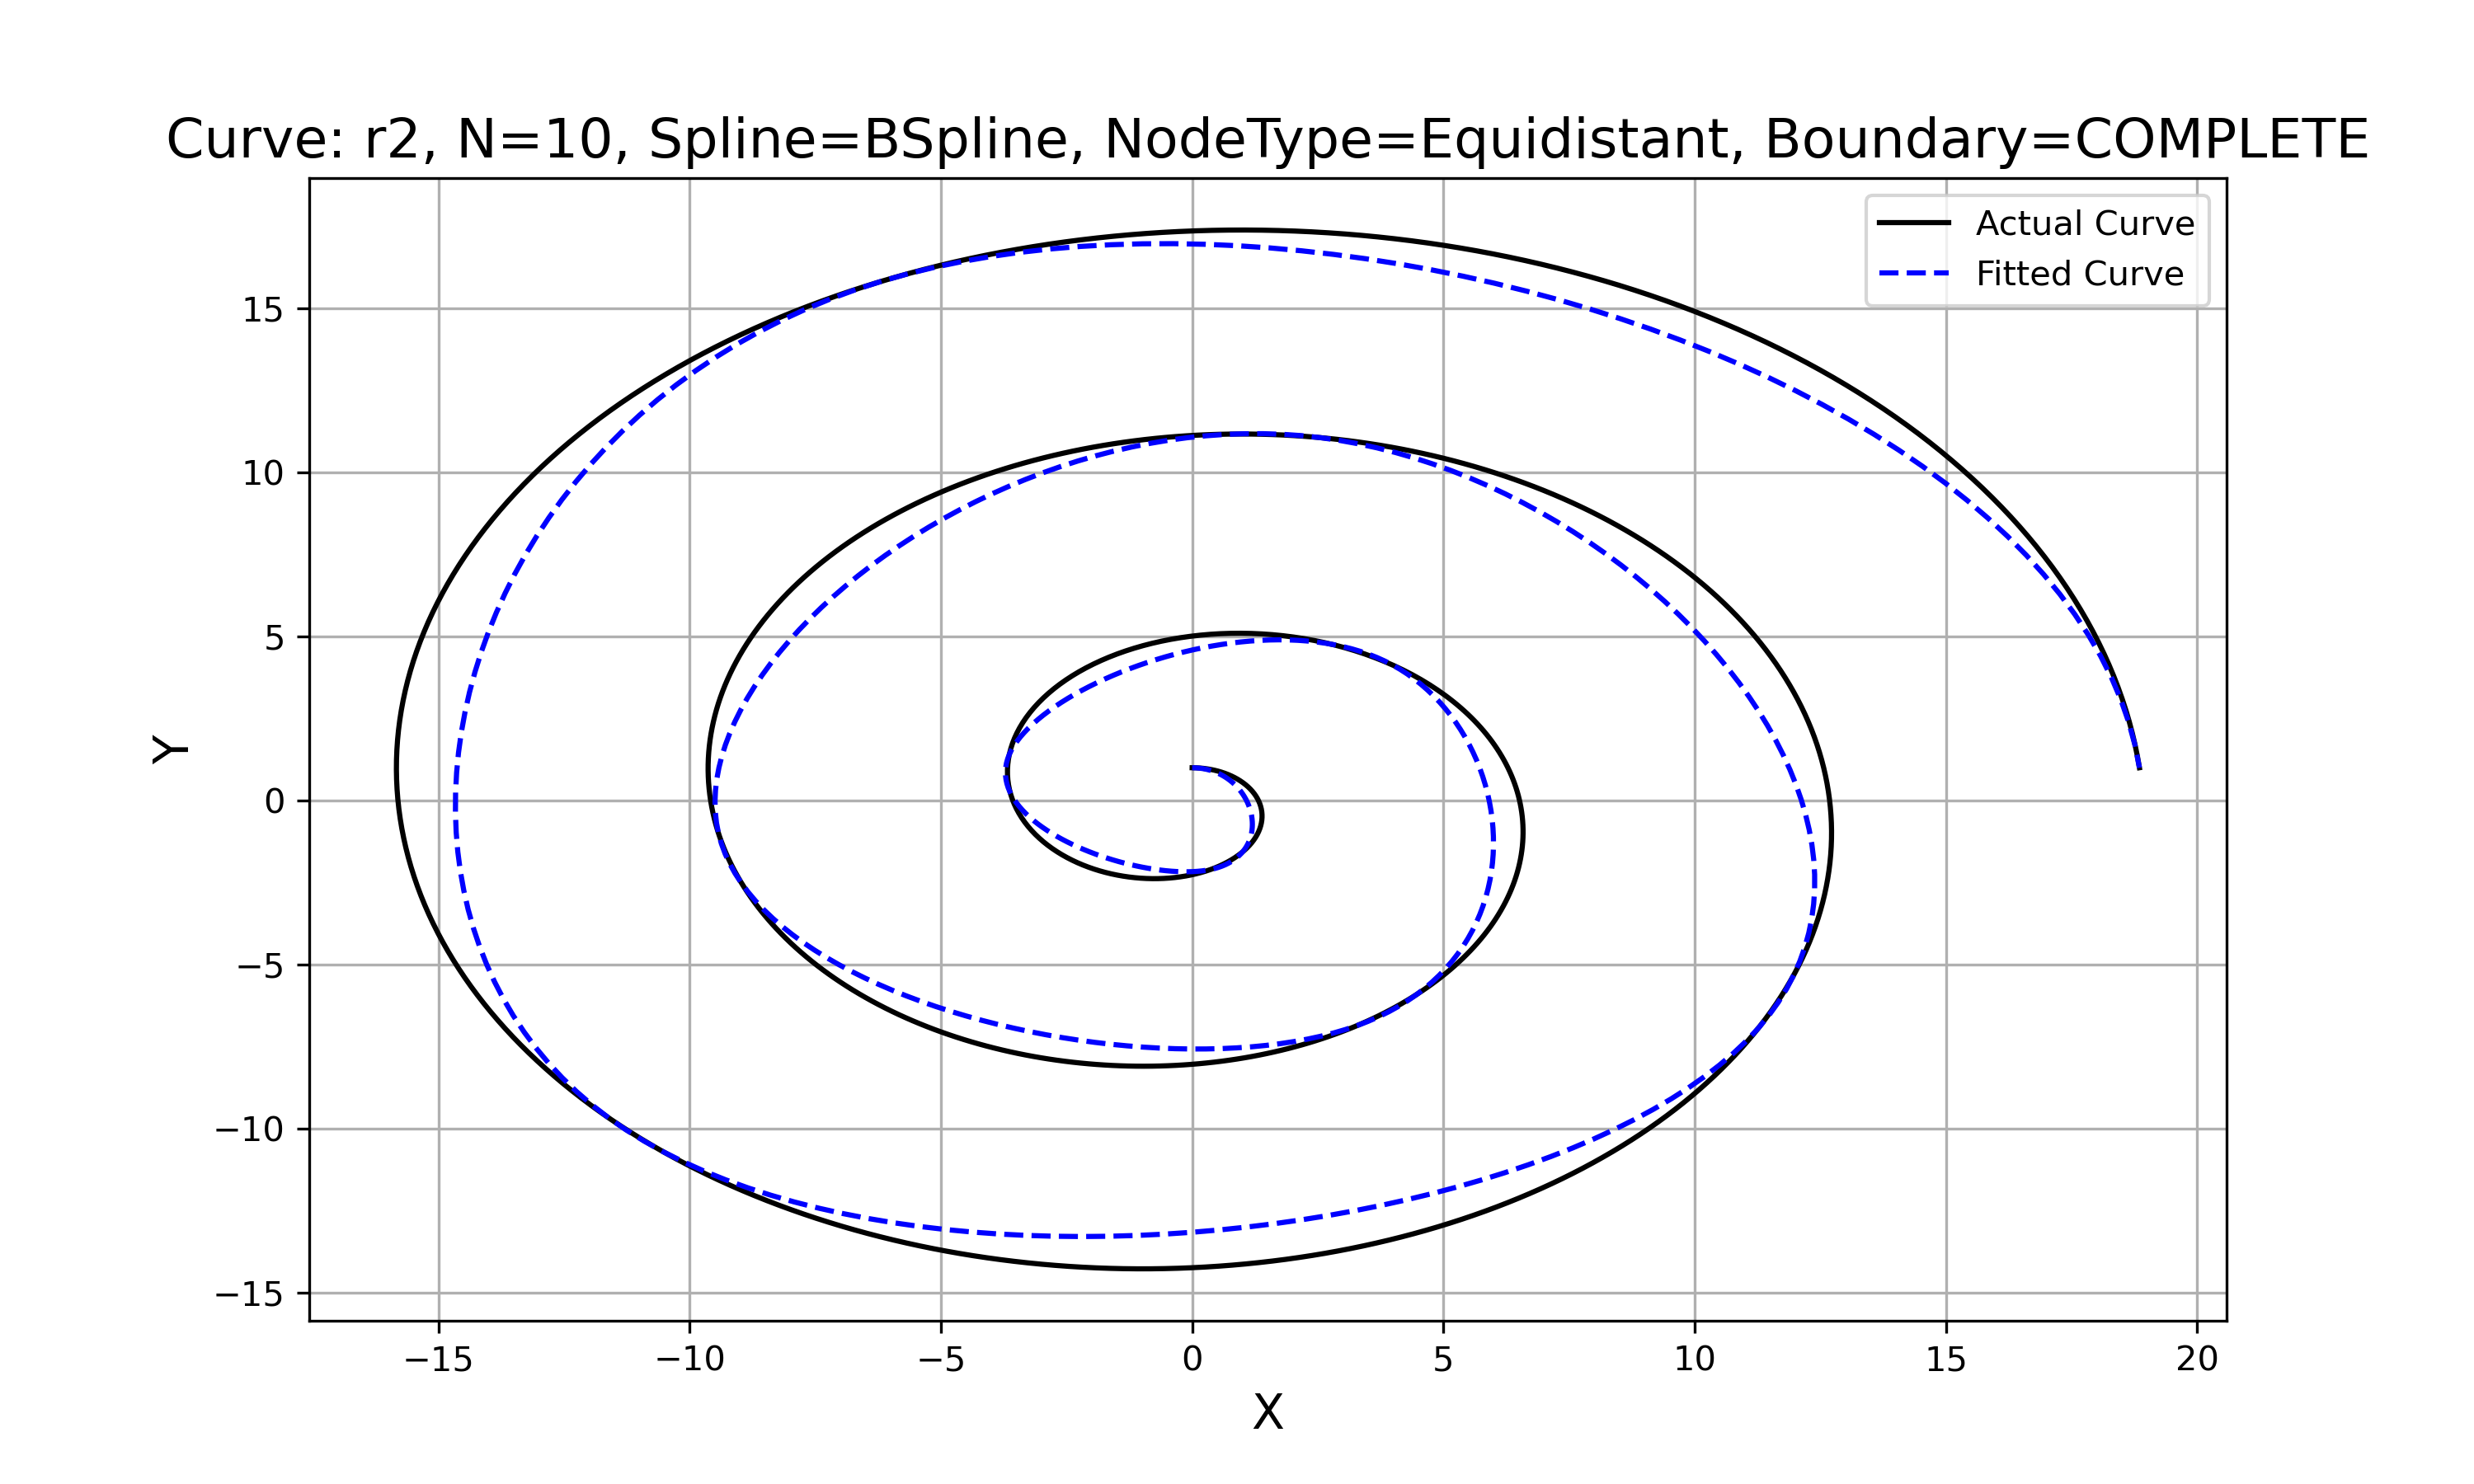
\includegraphics[width=0.45\textwidth]{../figure/problemE/N_10_r2_BSpline_Equidistant_COMPLETE.png}  &
    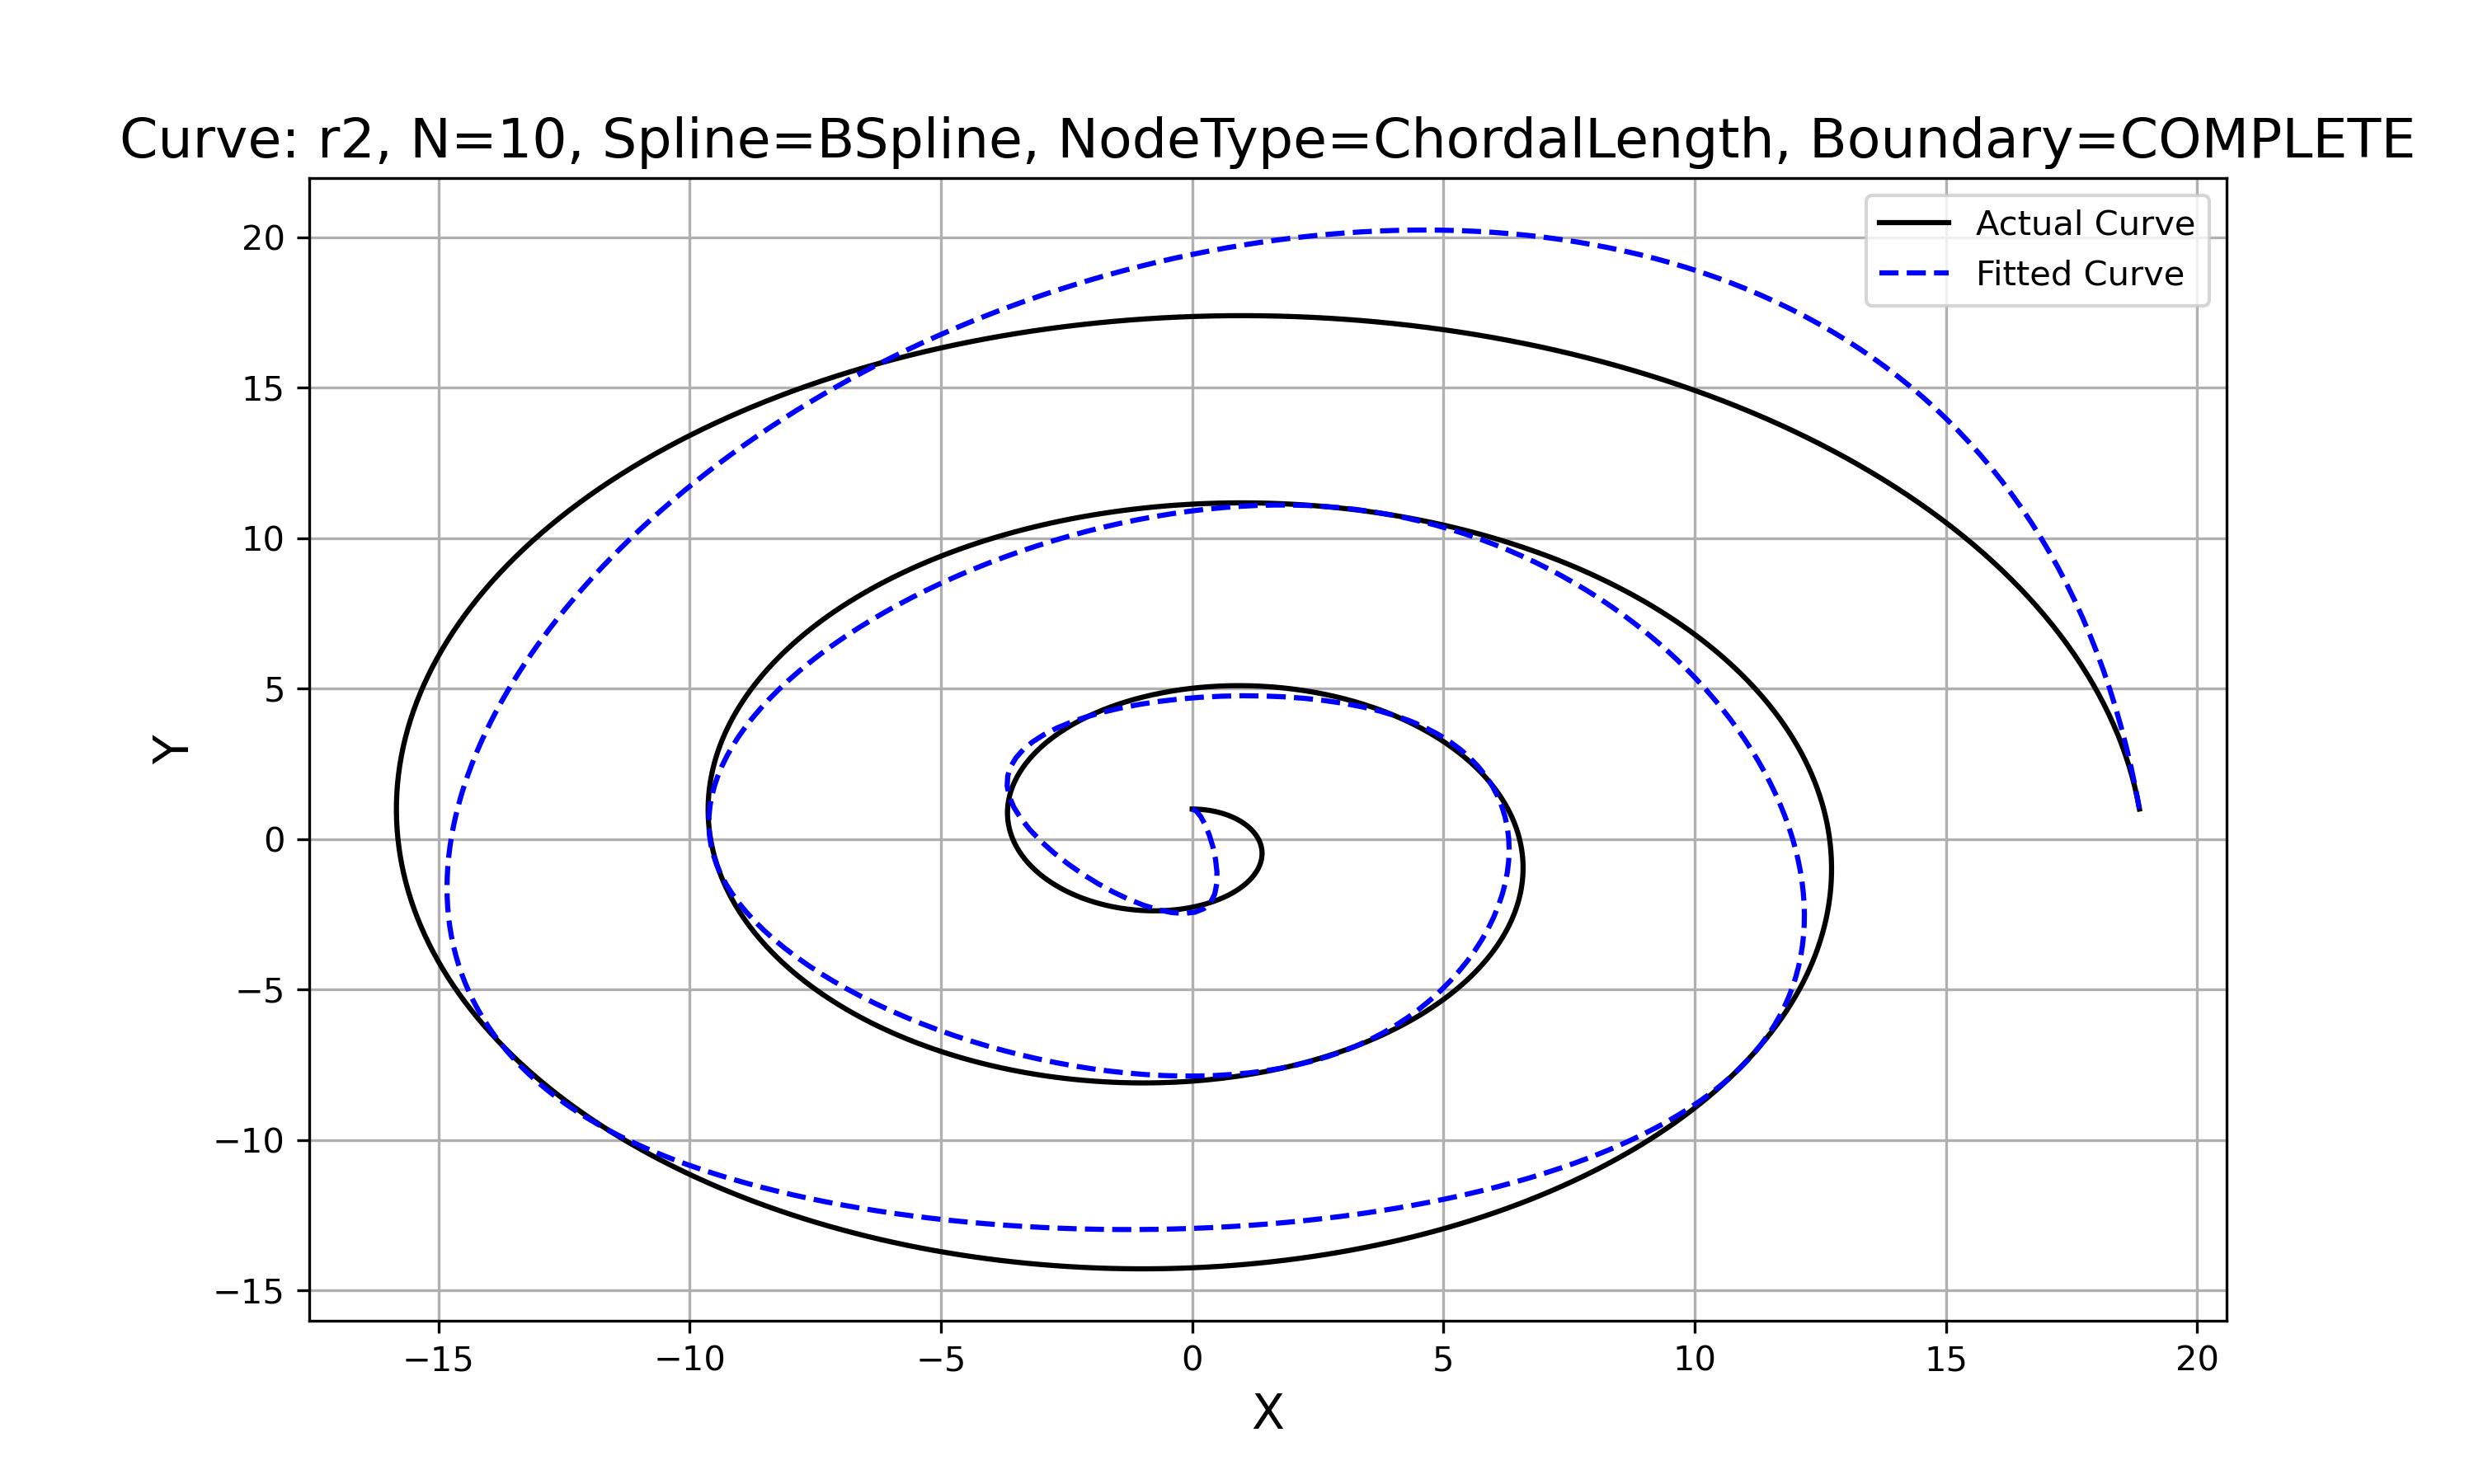
\includegraphics[width=0.45\textwidth]{../figure/problemE/N_10_r2_BSpline_ChordalLength_COMPLETE.png}  \\
    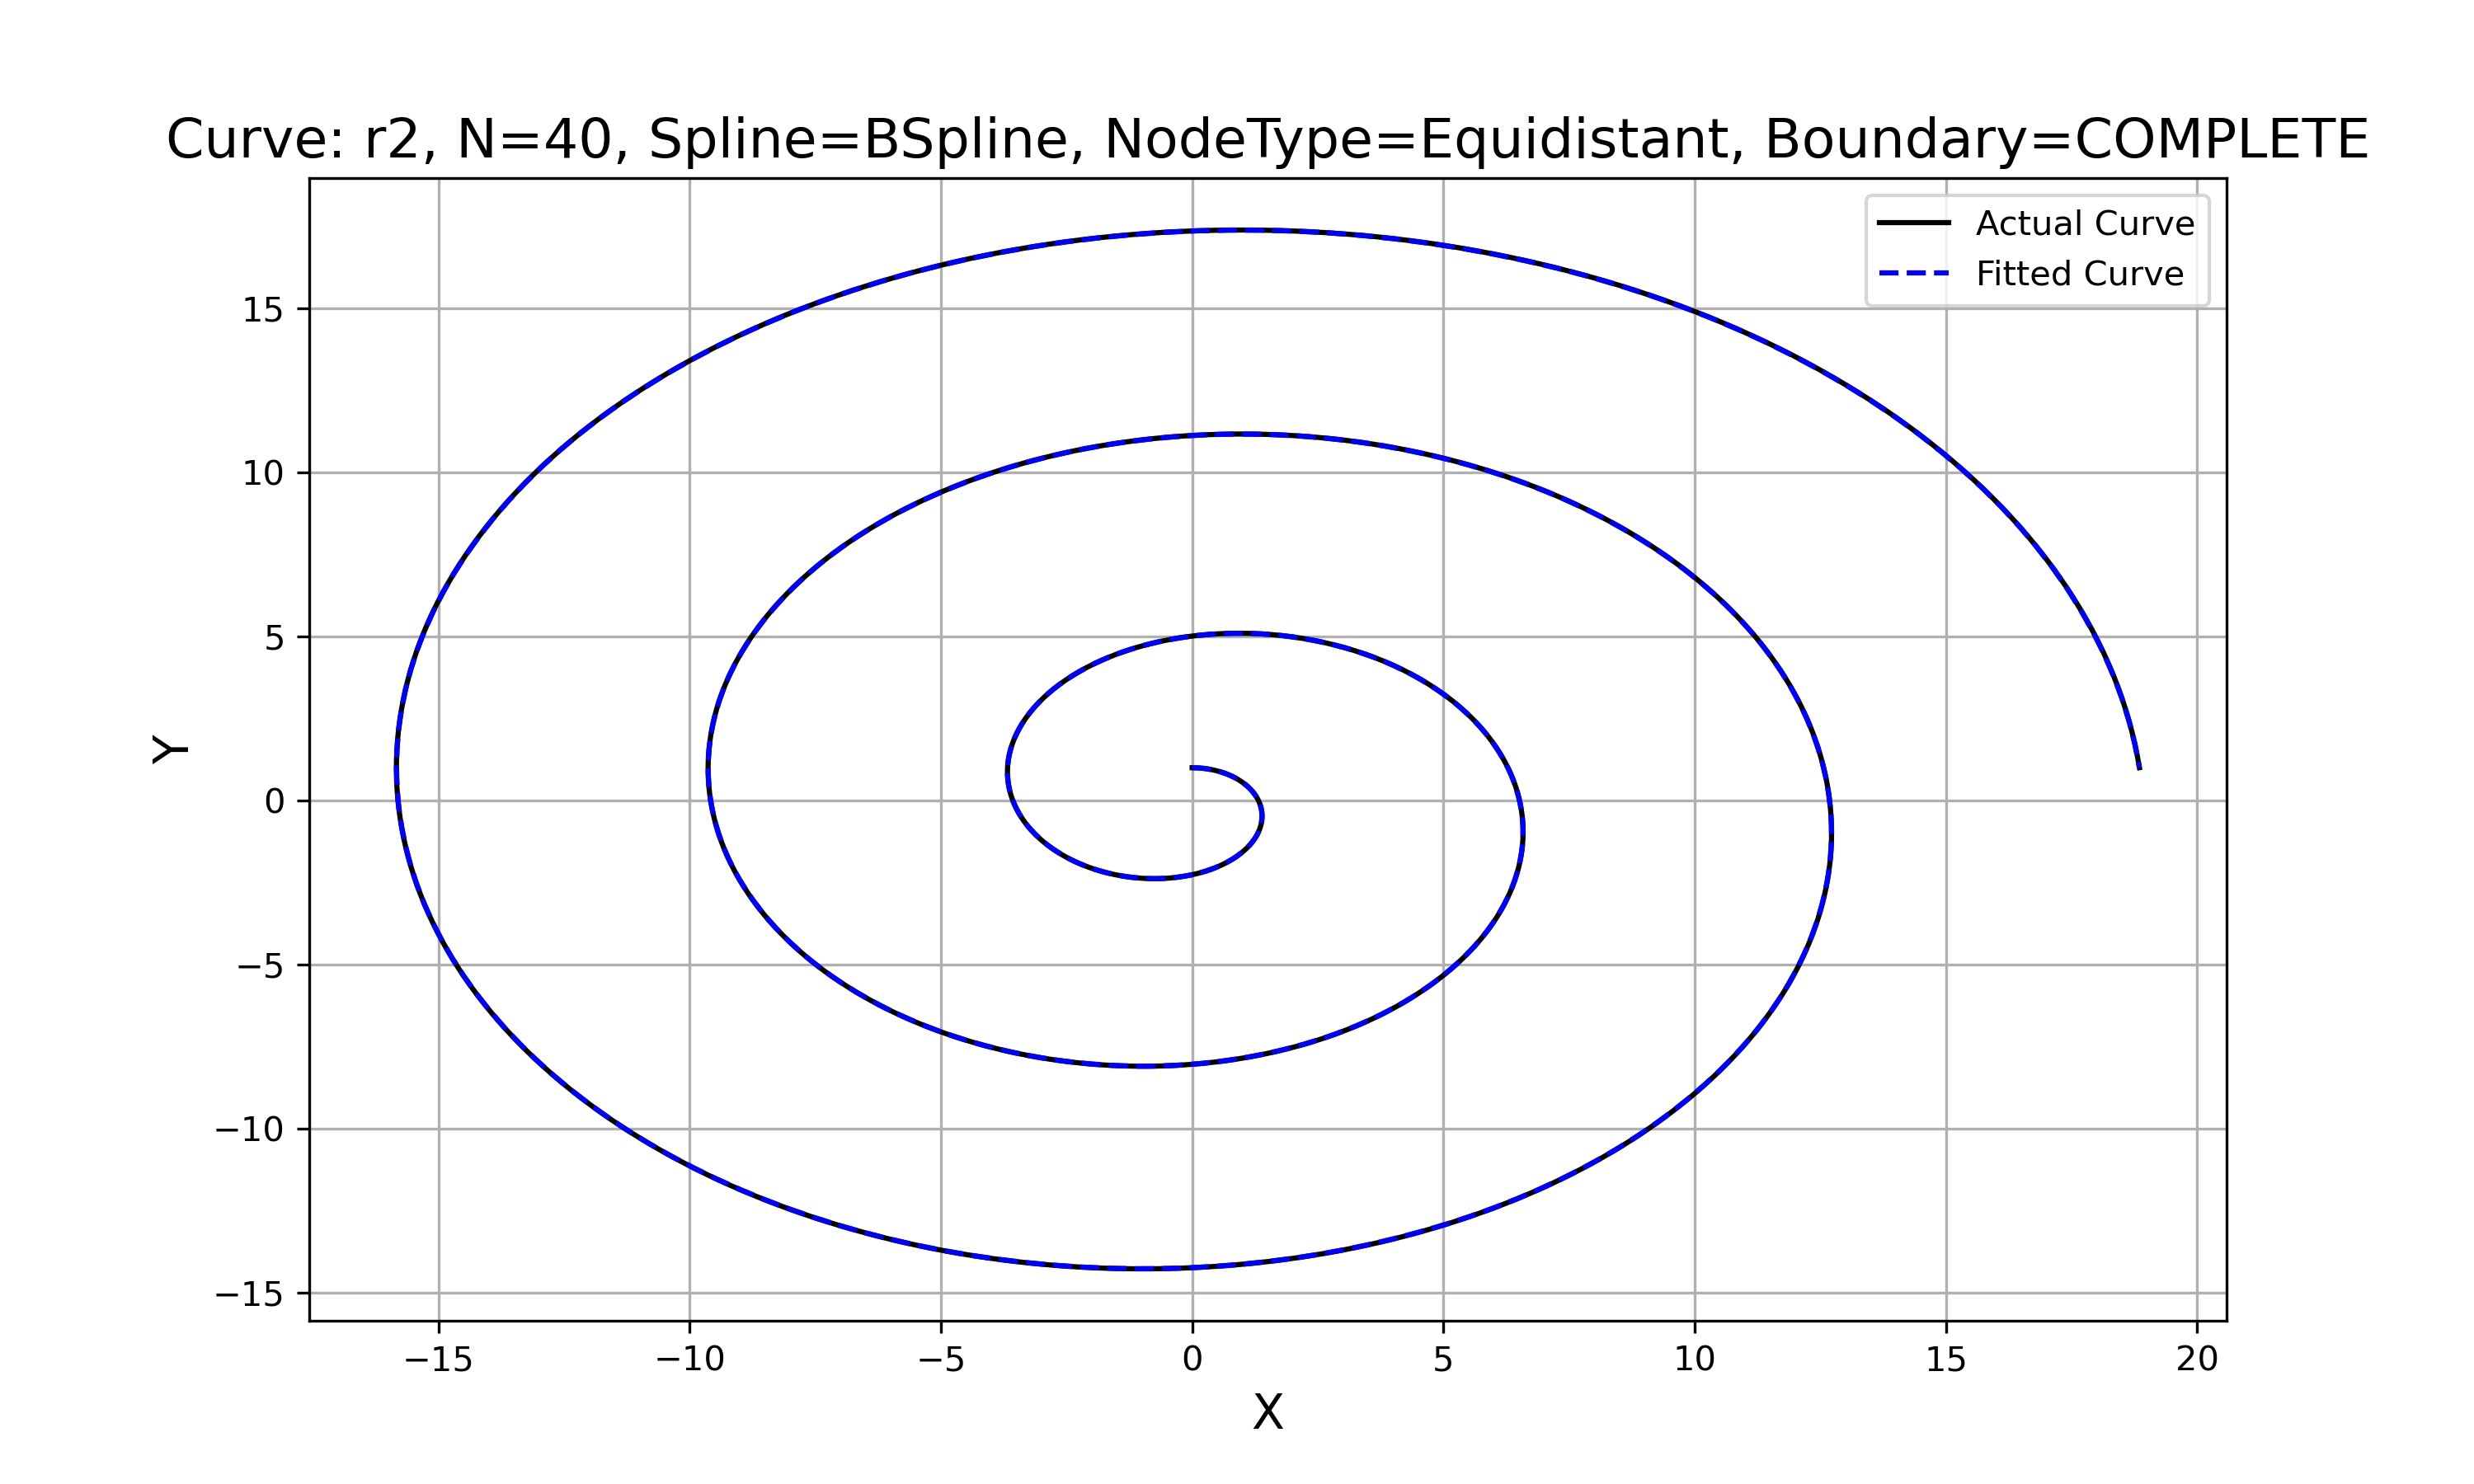
\includegraphics[width=0.45\textwidth]{../figure/problemE/N_40_r2_BSpline_Equidistant_COMPLETE.png}  &
    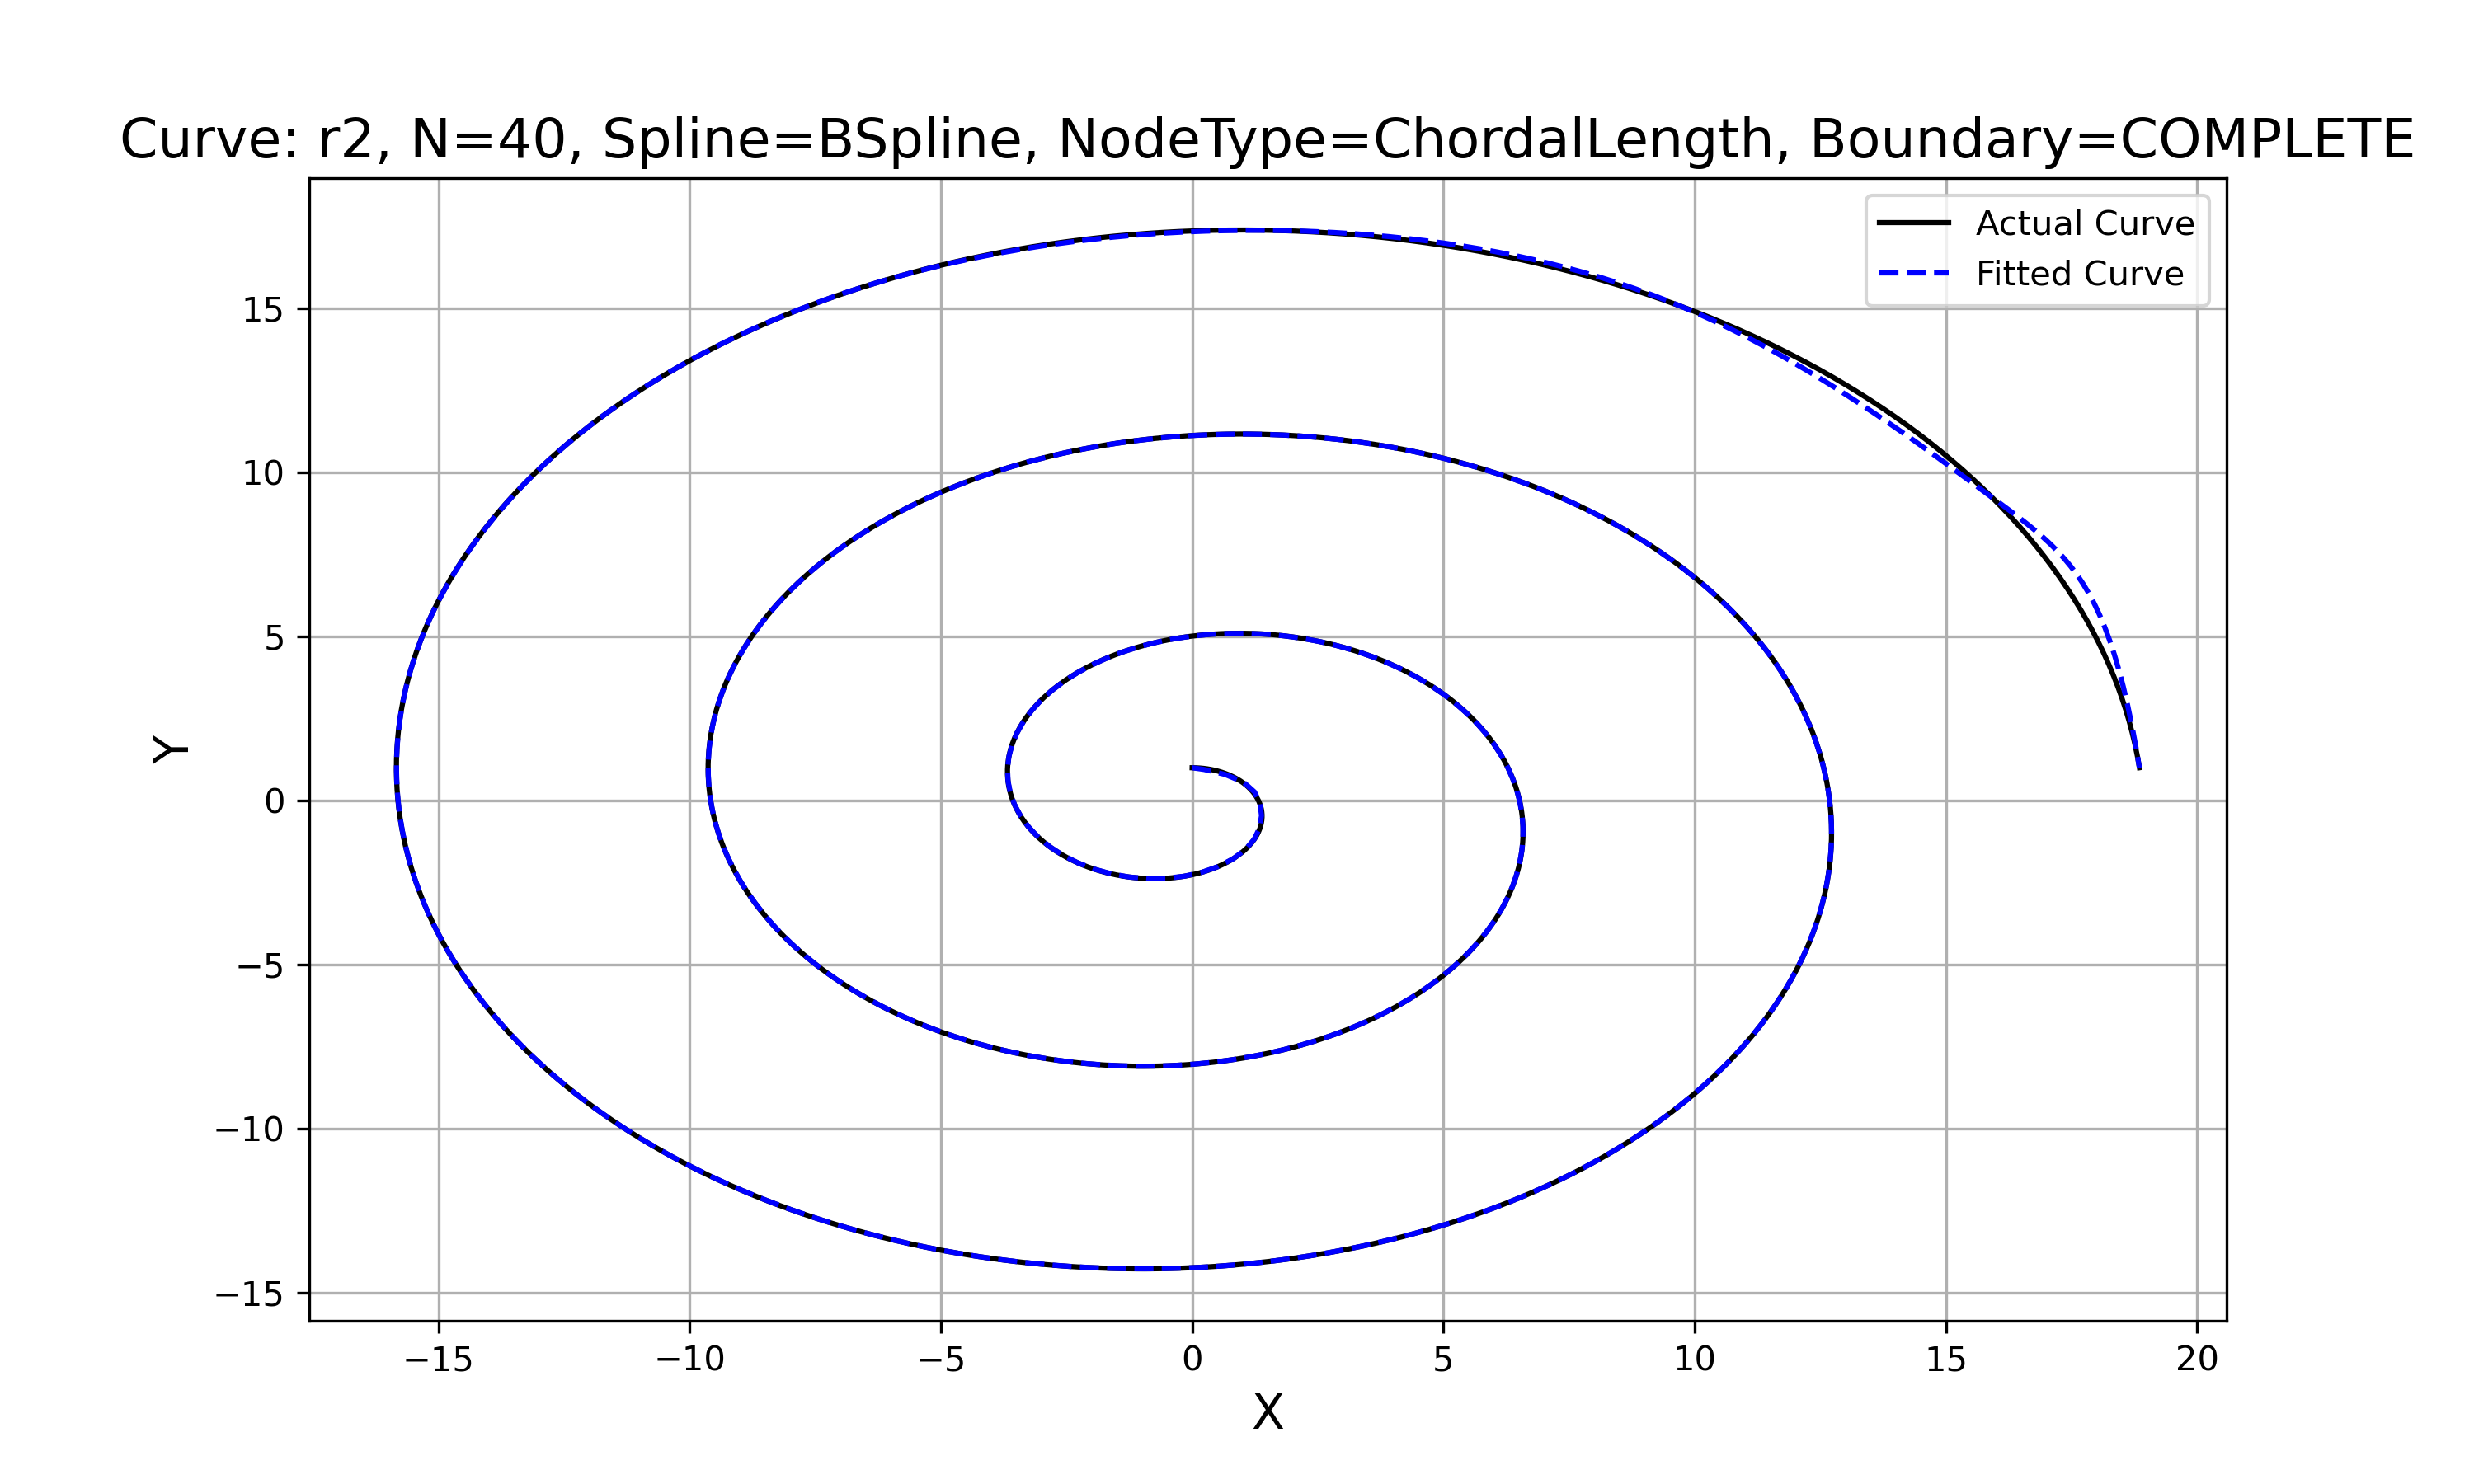
\includegraphics[width=0.45\textwidth]{../figure/problemE/N_40_r2_BSpline_ChordalLength_COMPLETE.png}  \\
    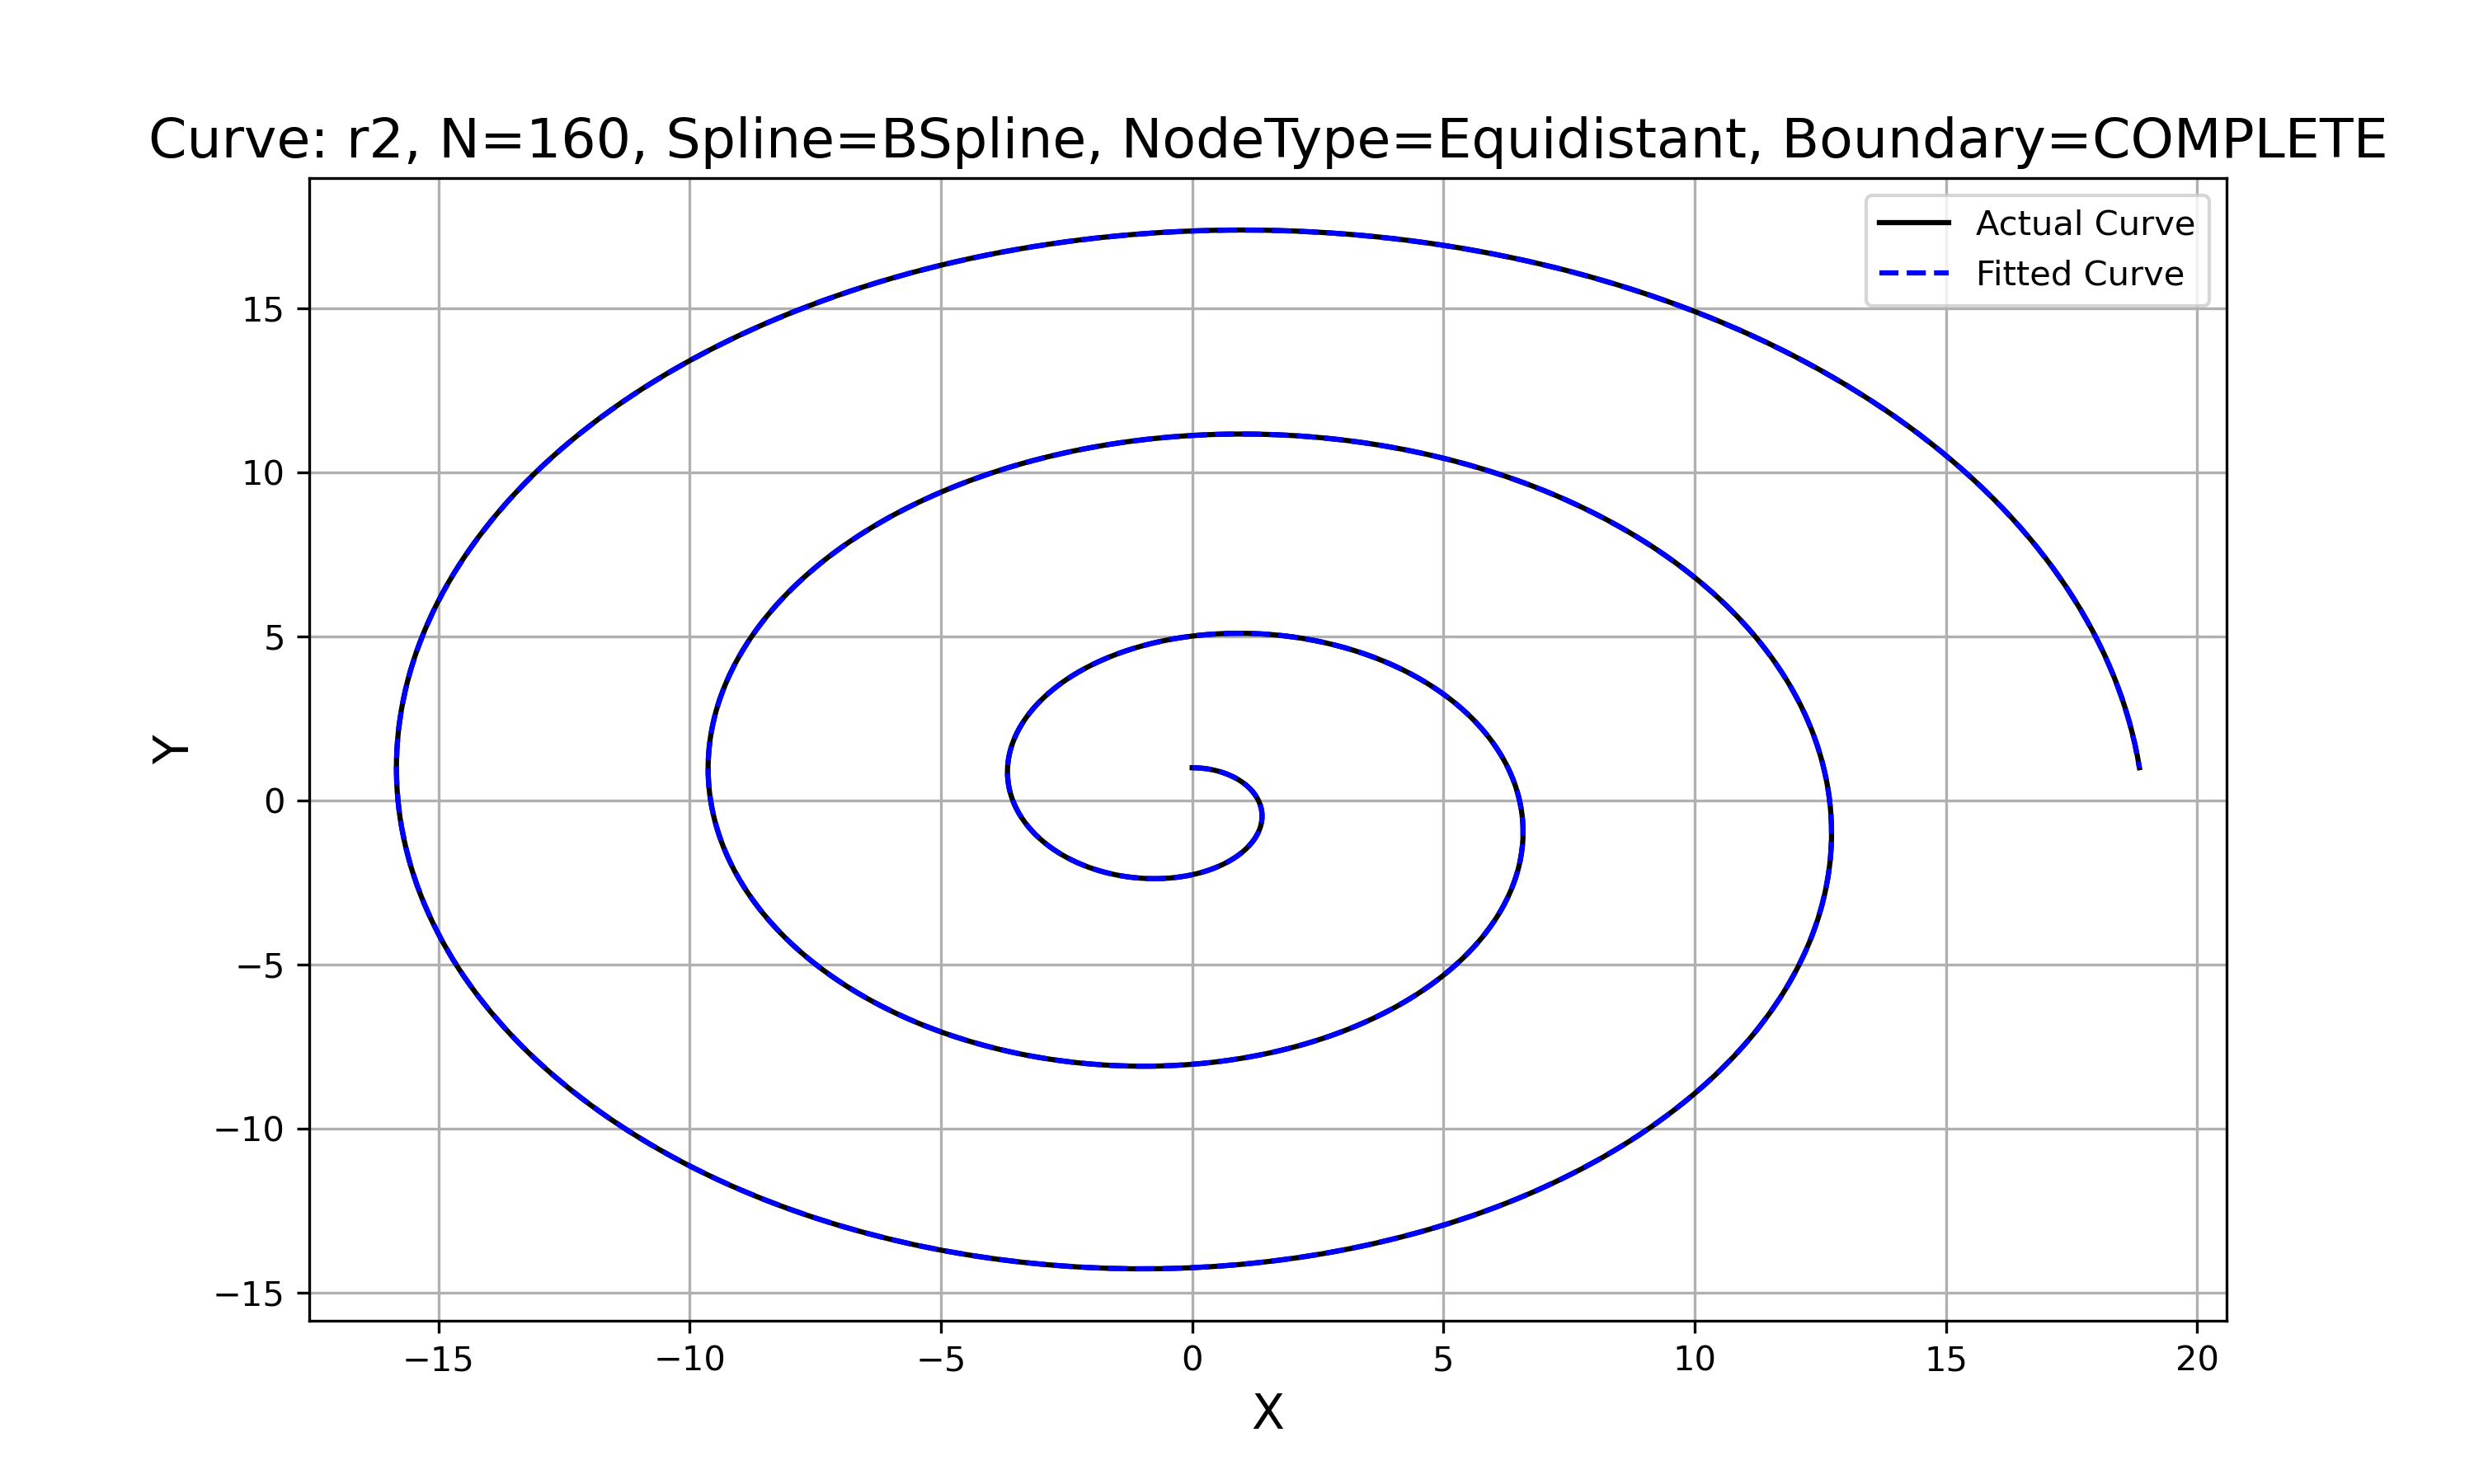
\includegraphics[width=0.45\textwidth]{../figure/problemE/N_160_r2_BSpline_Equidistant_COMPLETE.png} &
    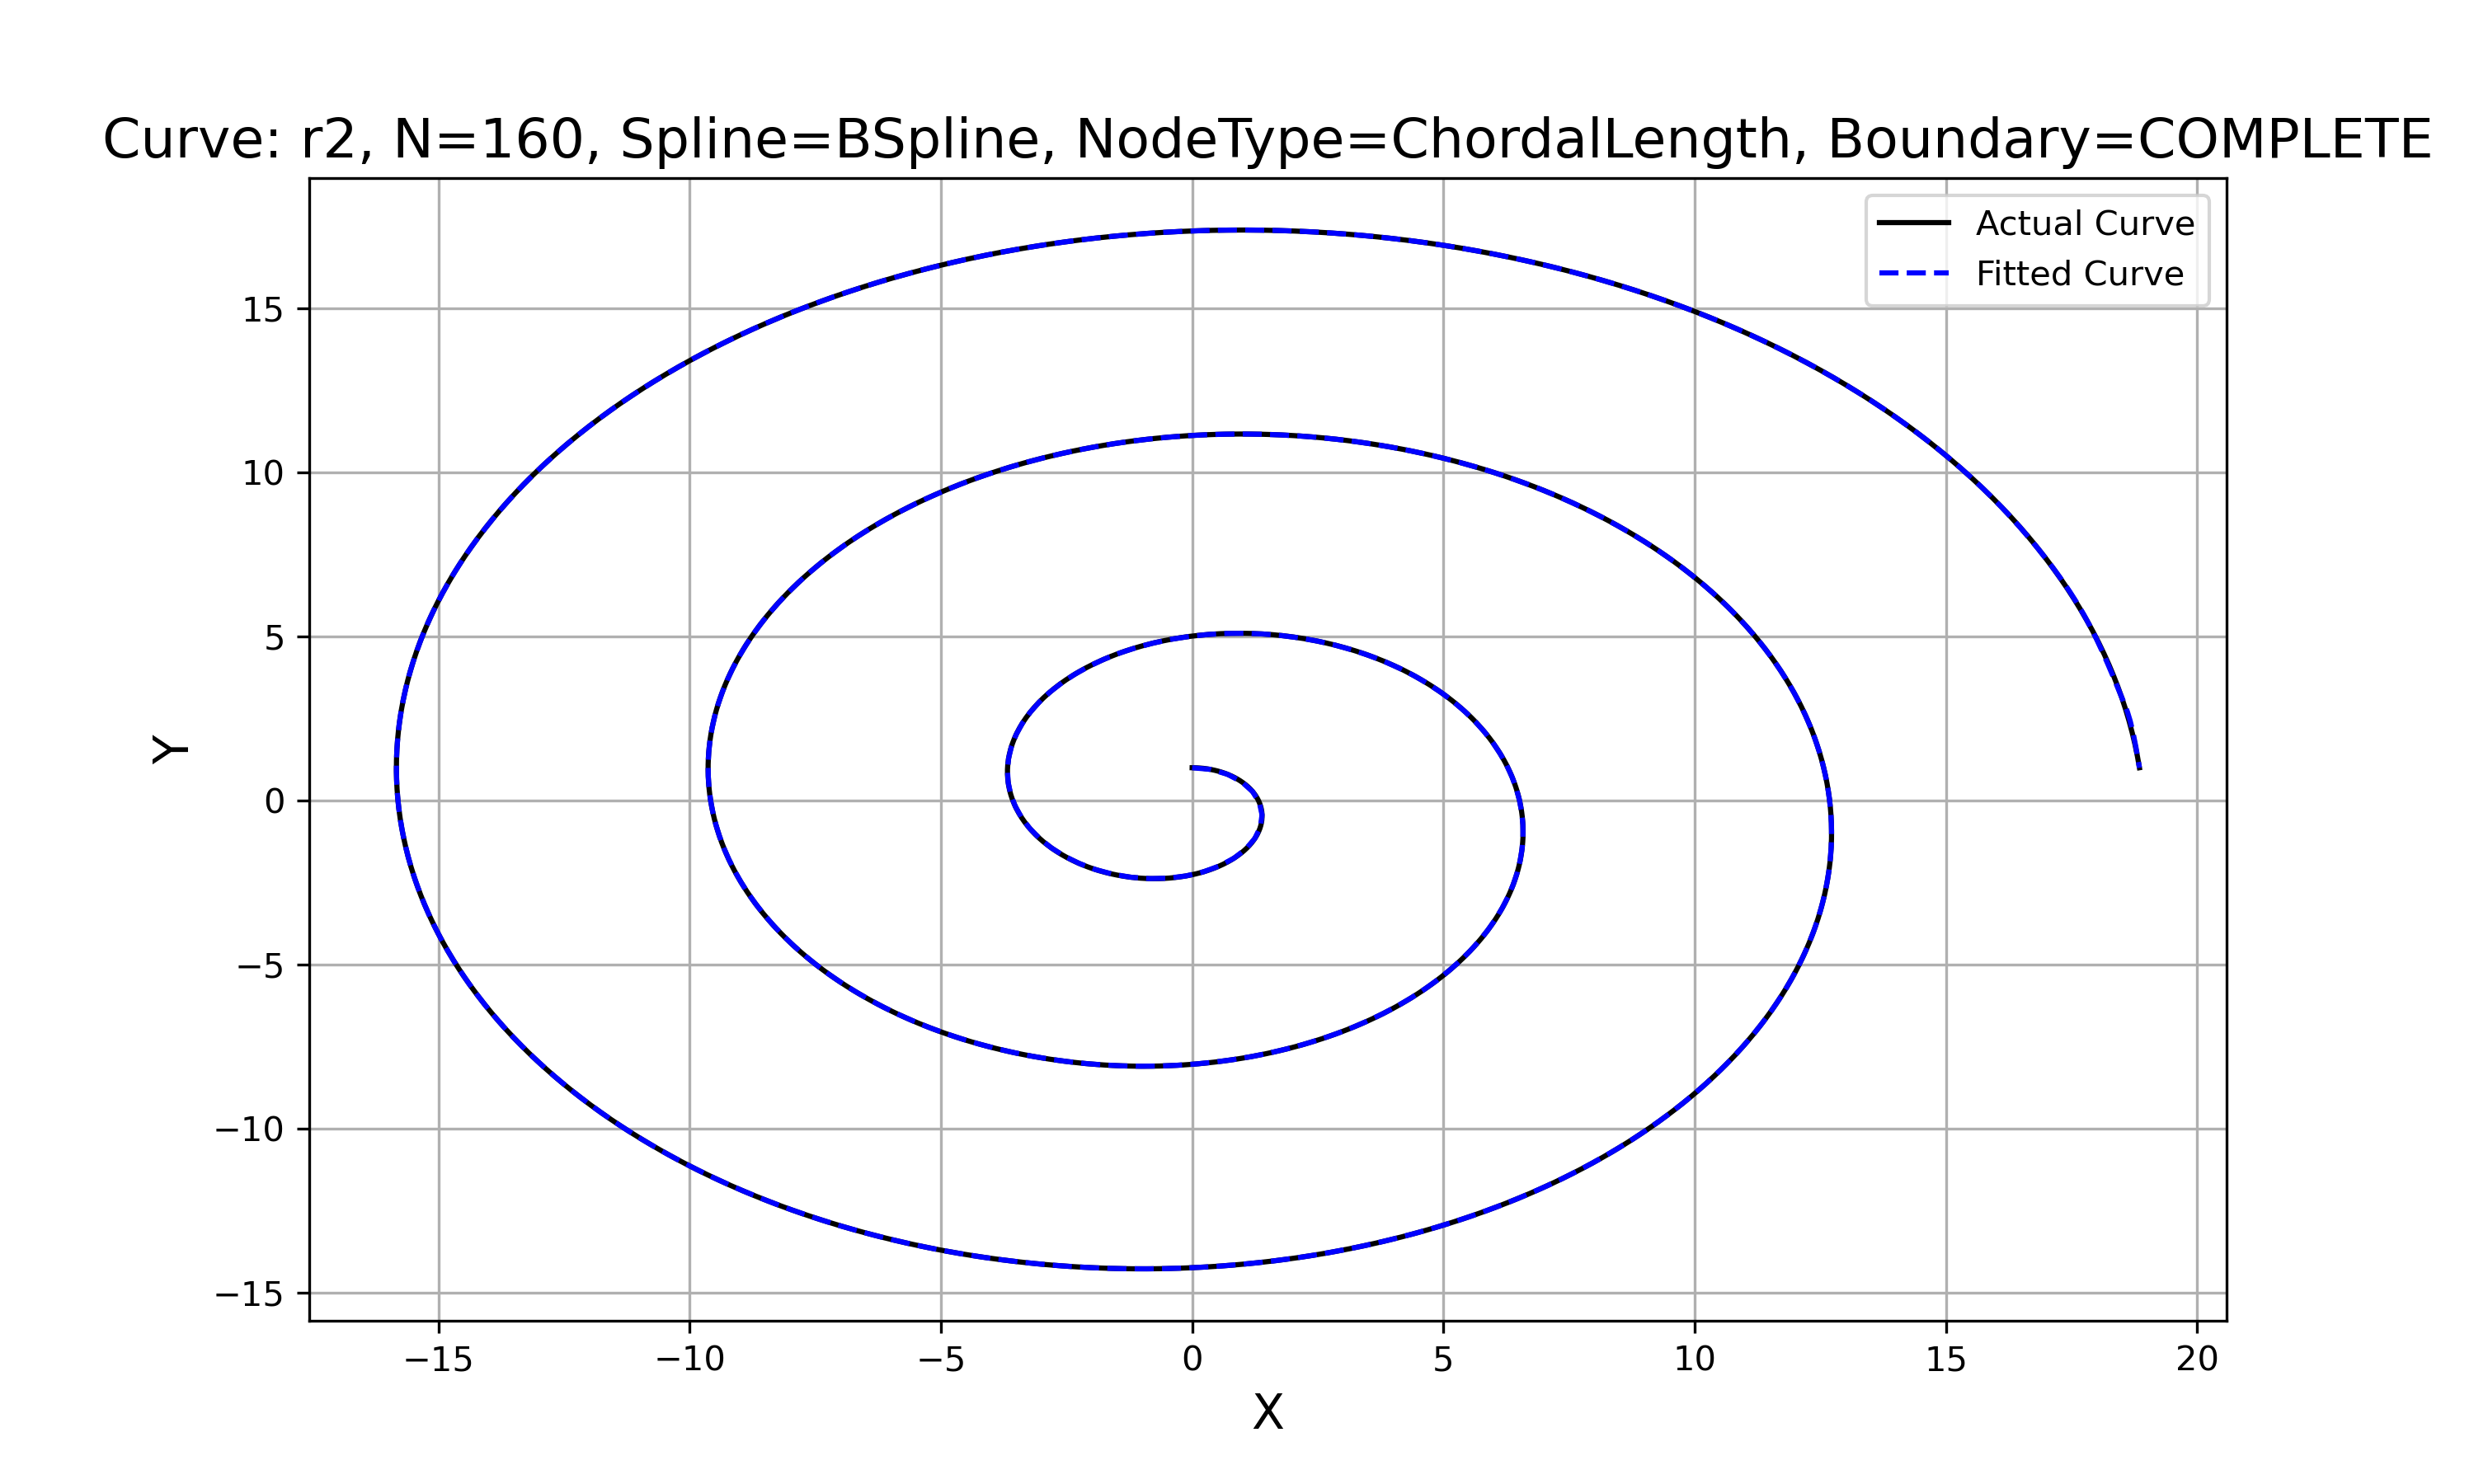
\includegraphics[width=0.45\textwidth]{../figure/problemE/N_160_r2_BSpline_ChordalLength_COMPLETE.png} \\
  \end{tabular}
  \renewcommand{\figurename}{Fig.}
  \caption{Comparison of Equidistant and Chordal Length for curve \(r_2\) with COMPLETE boundary condition}
  \label{fig:r2_nodeType_compare}
\end{figure}

The fitting effect of curve \(r_2\) is shown in
Fig.\ref{fig:r2_nodeType_compare}. This spiral curve is relatively smooth, so a
small number of equidistant nodes can achieve a good fitting effect. However,
for the cumulative chordal length method, due to the approximation errors in
calculating the chord length, the fitting effect at the ends is poor when the
number of data points is small. Therefore, more data points are needed to
ensure a good fitting effect.

\begin{figure}[H]
  \centering
  \begin{tabular}{cc}
    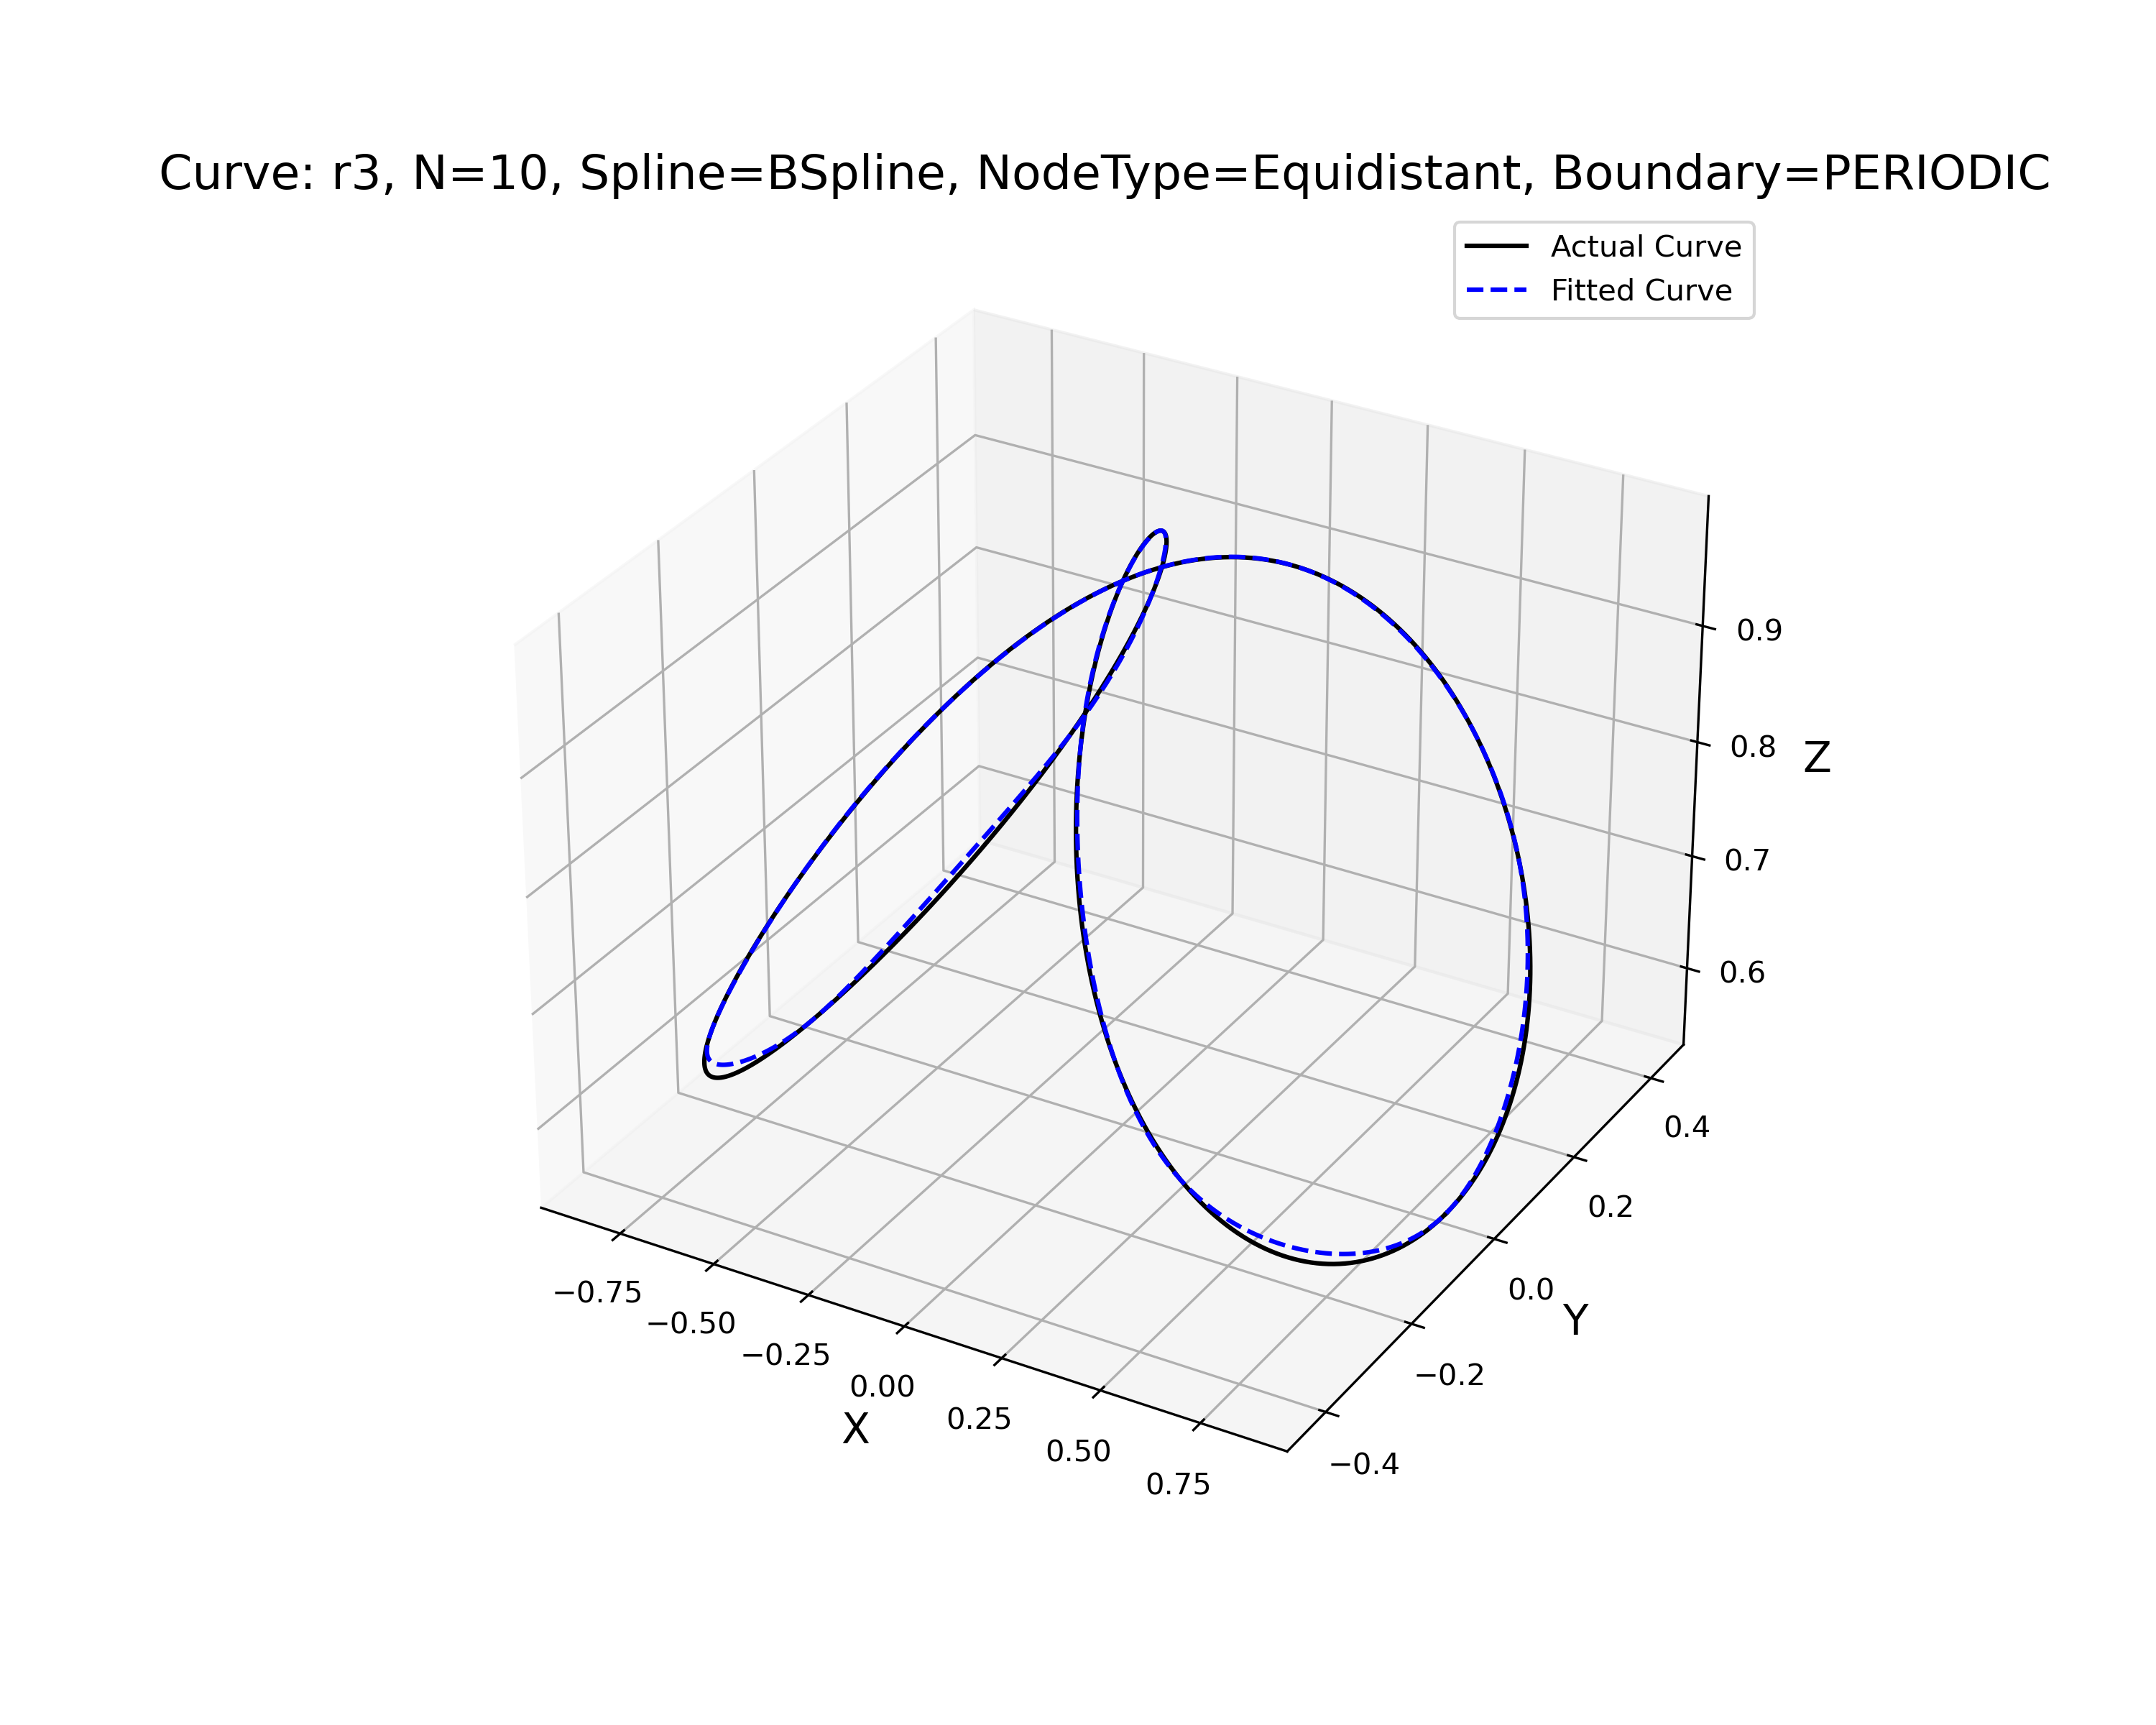
\includegraphics[width=0.45\textwidth]{../figure/problemE/N_10_r3_BSpline_Equidistant_PERIODIC_3D.png}  &
    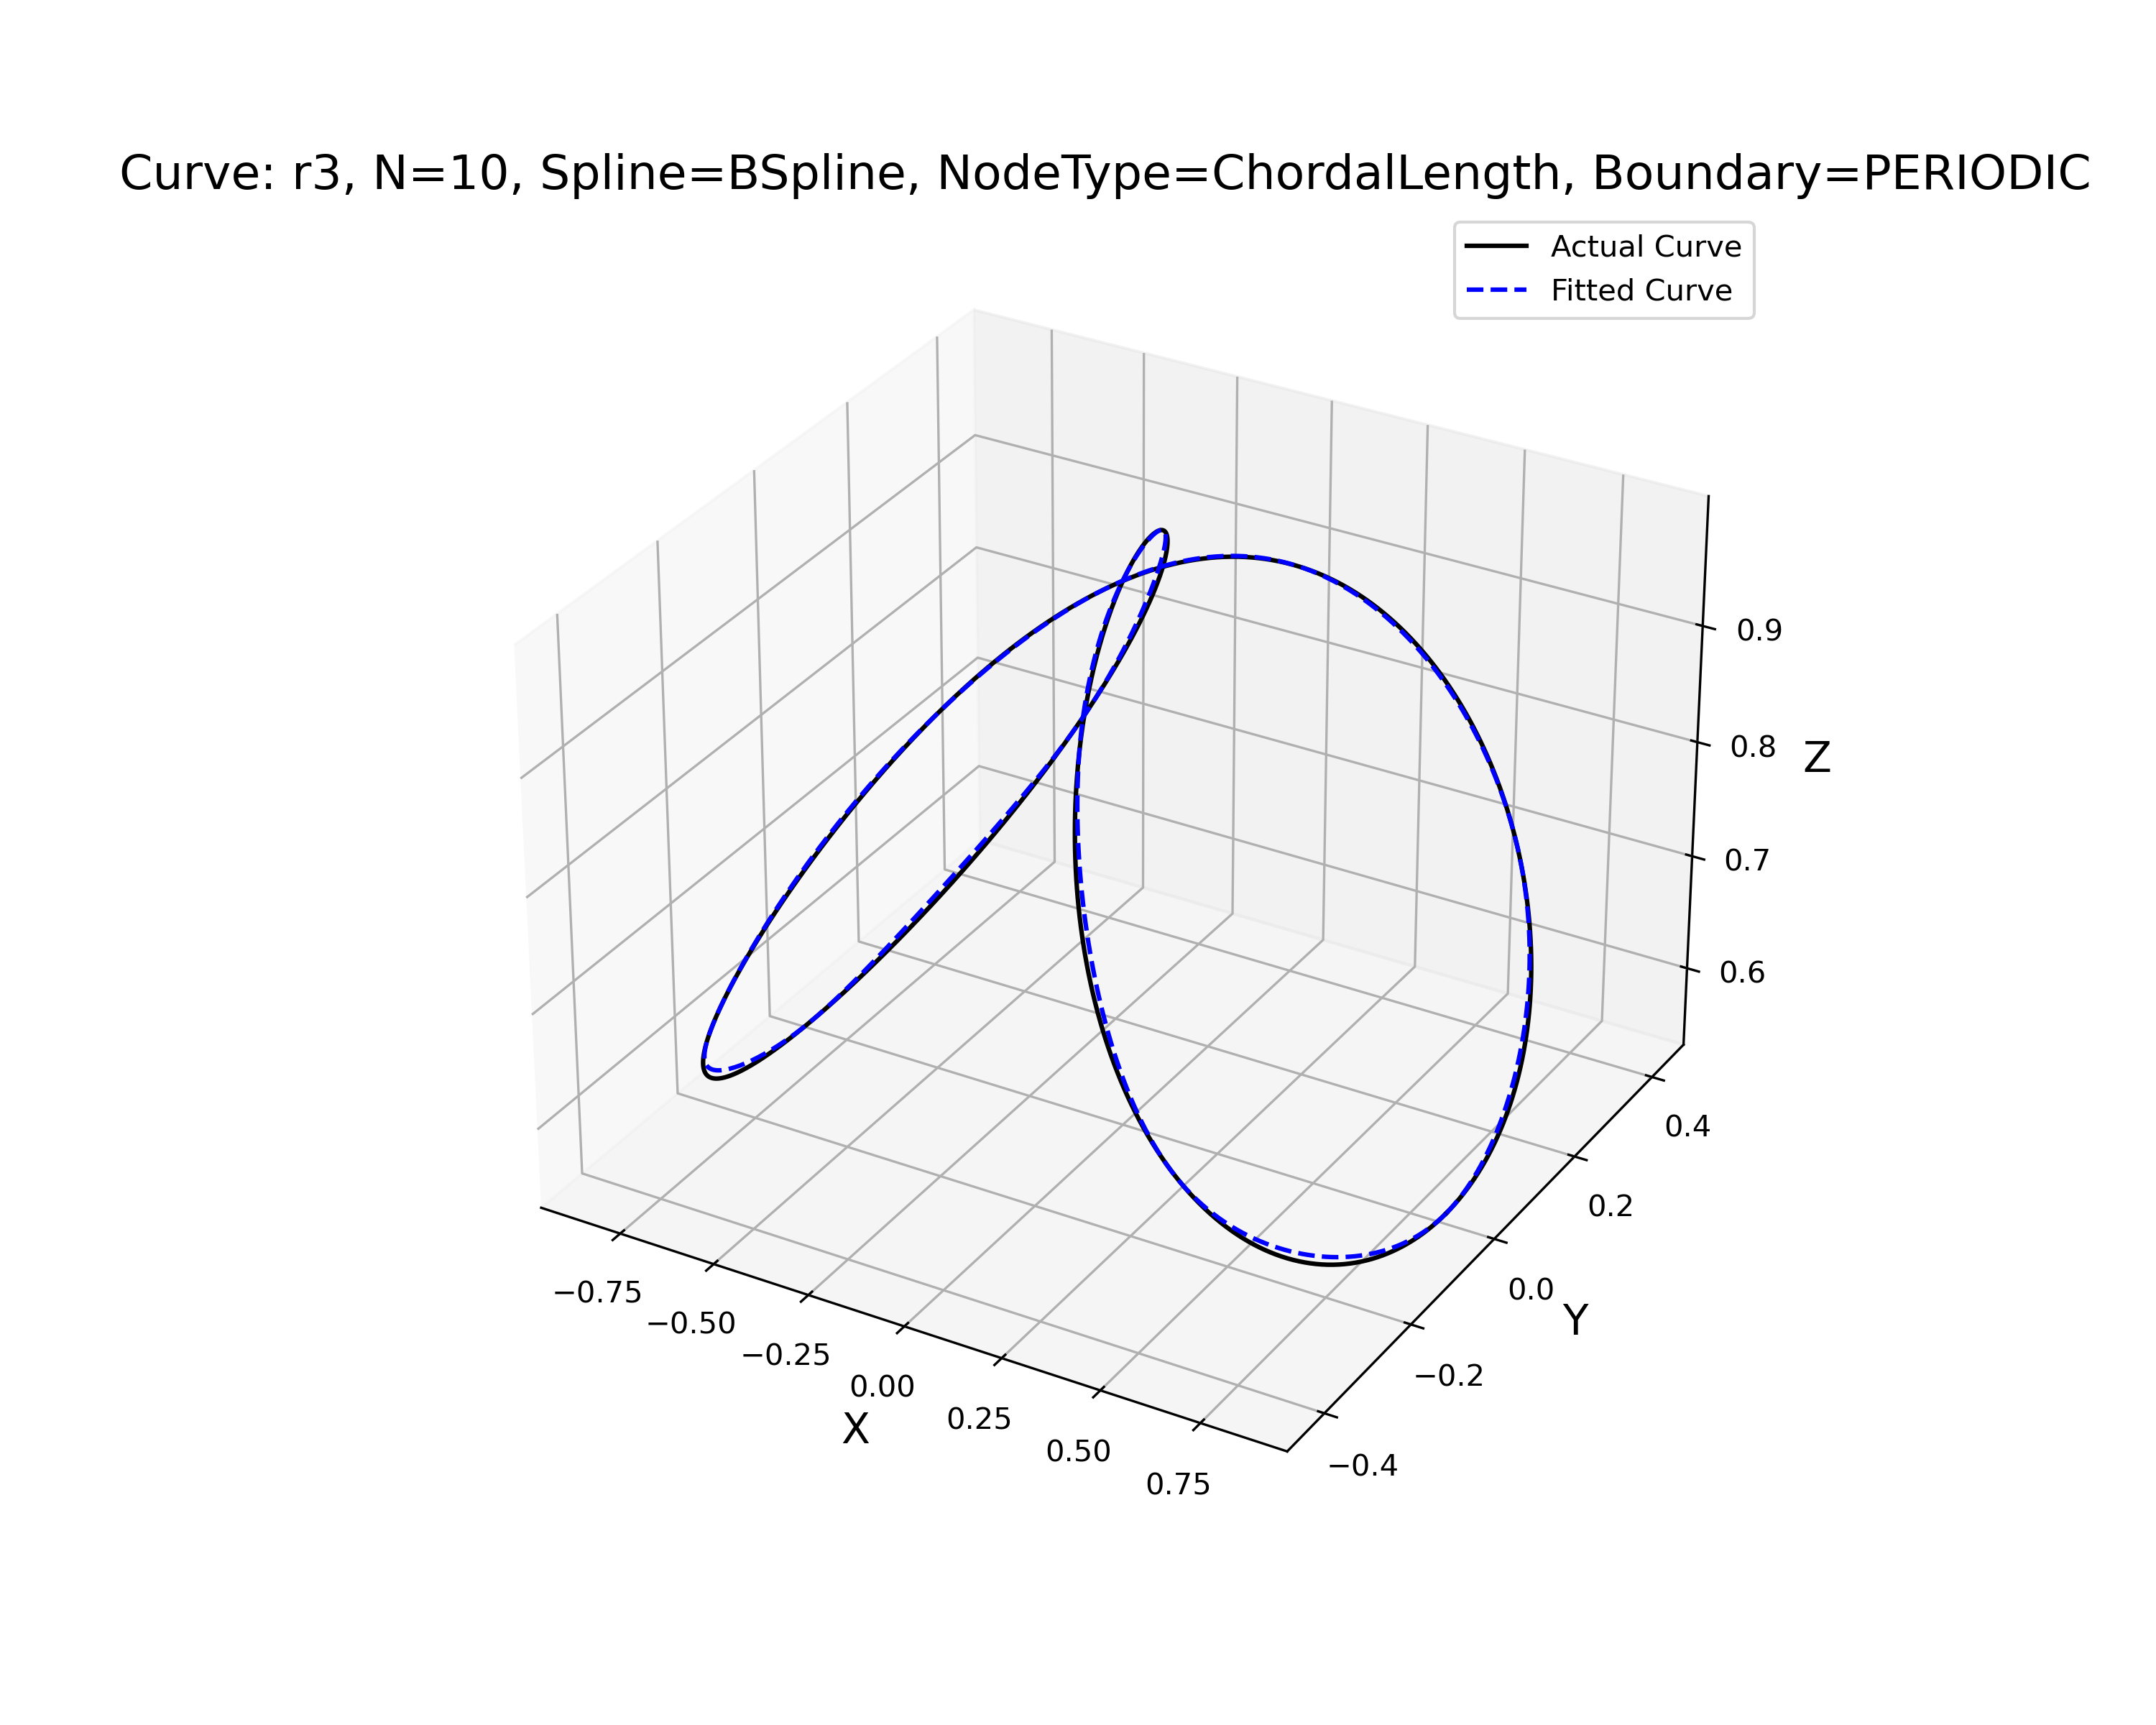
\includegraphics[width=0.45\textwidth]{../figure/problemE/N_10_r3_BSpline_ChordalLength_PERIODIC_3D.png}  \\
    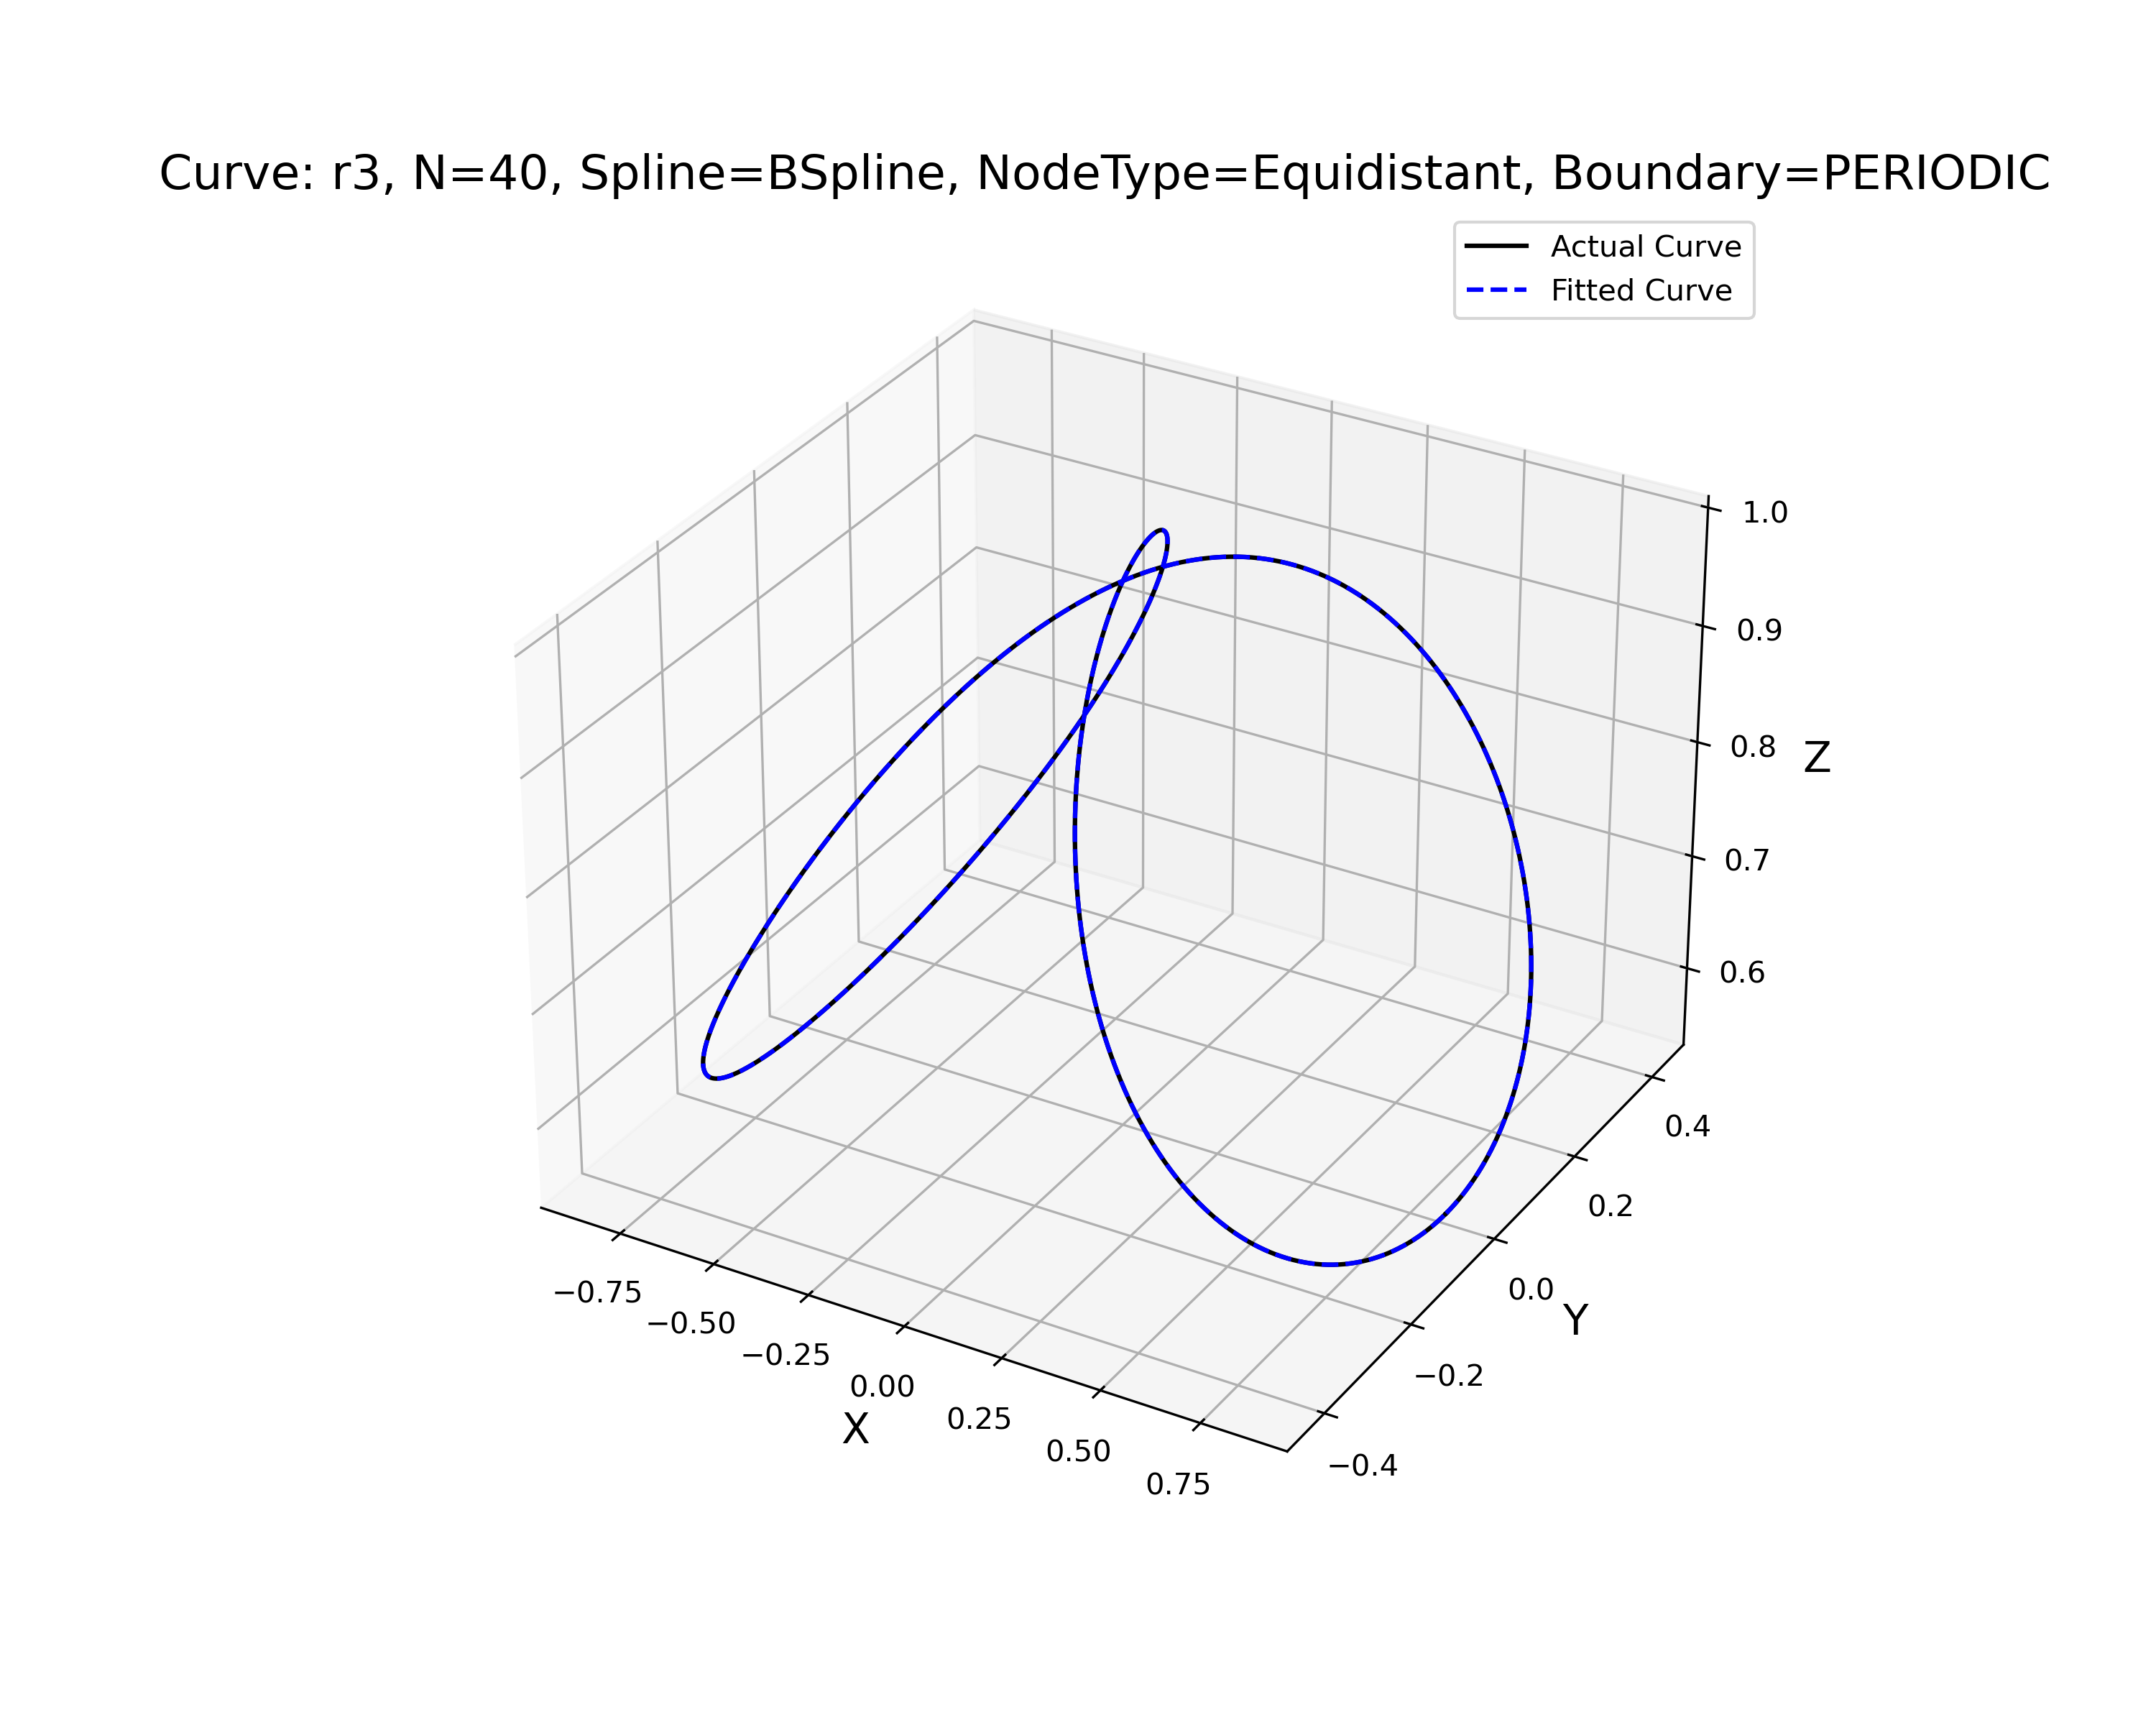
\includegraphics[width=0.45\textwidth]{../figure/problemE/N_40_r3_BSpline_Equidistant_PERIODIC_3D.png}  &
    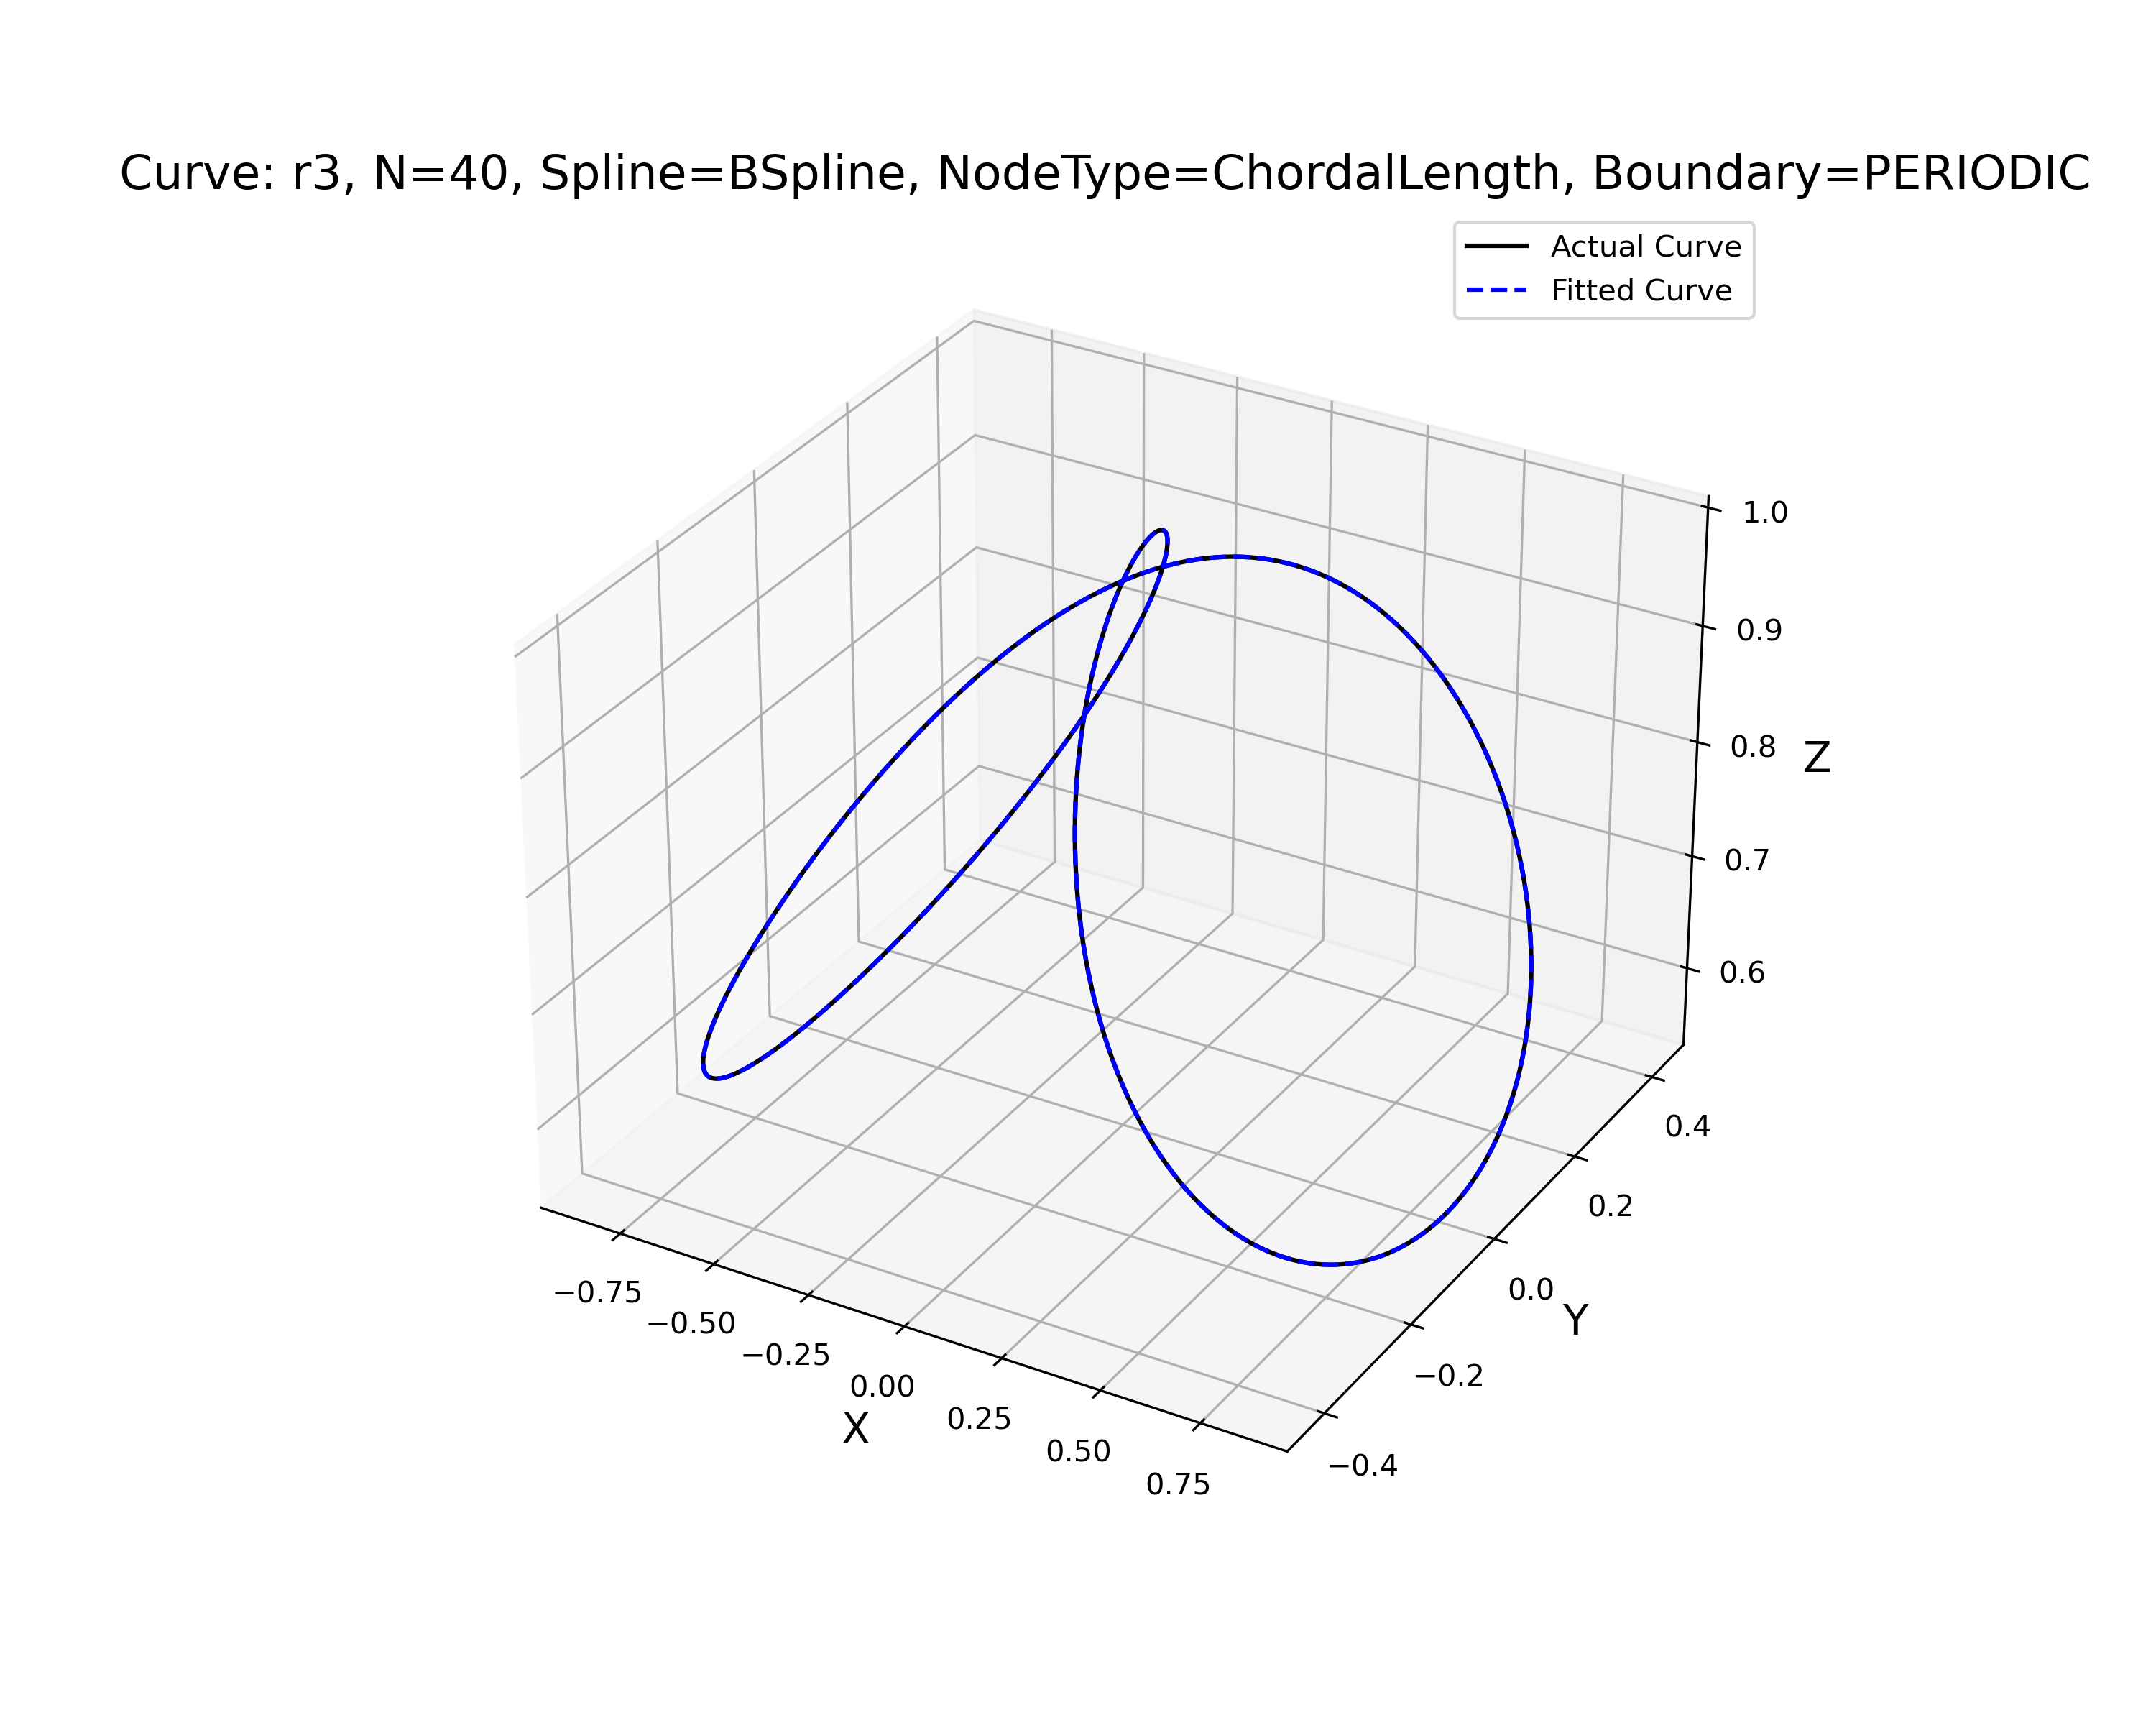
\includegraphics[width=0.45\textwidth]{../figure/problemE/N_40_r3_BSpline_ChordalLength_PERIODIC_3D.png}  \\
    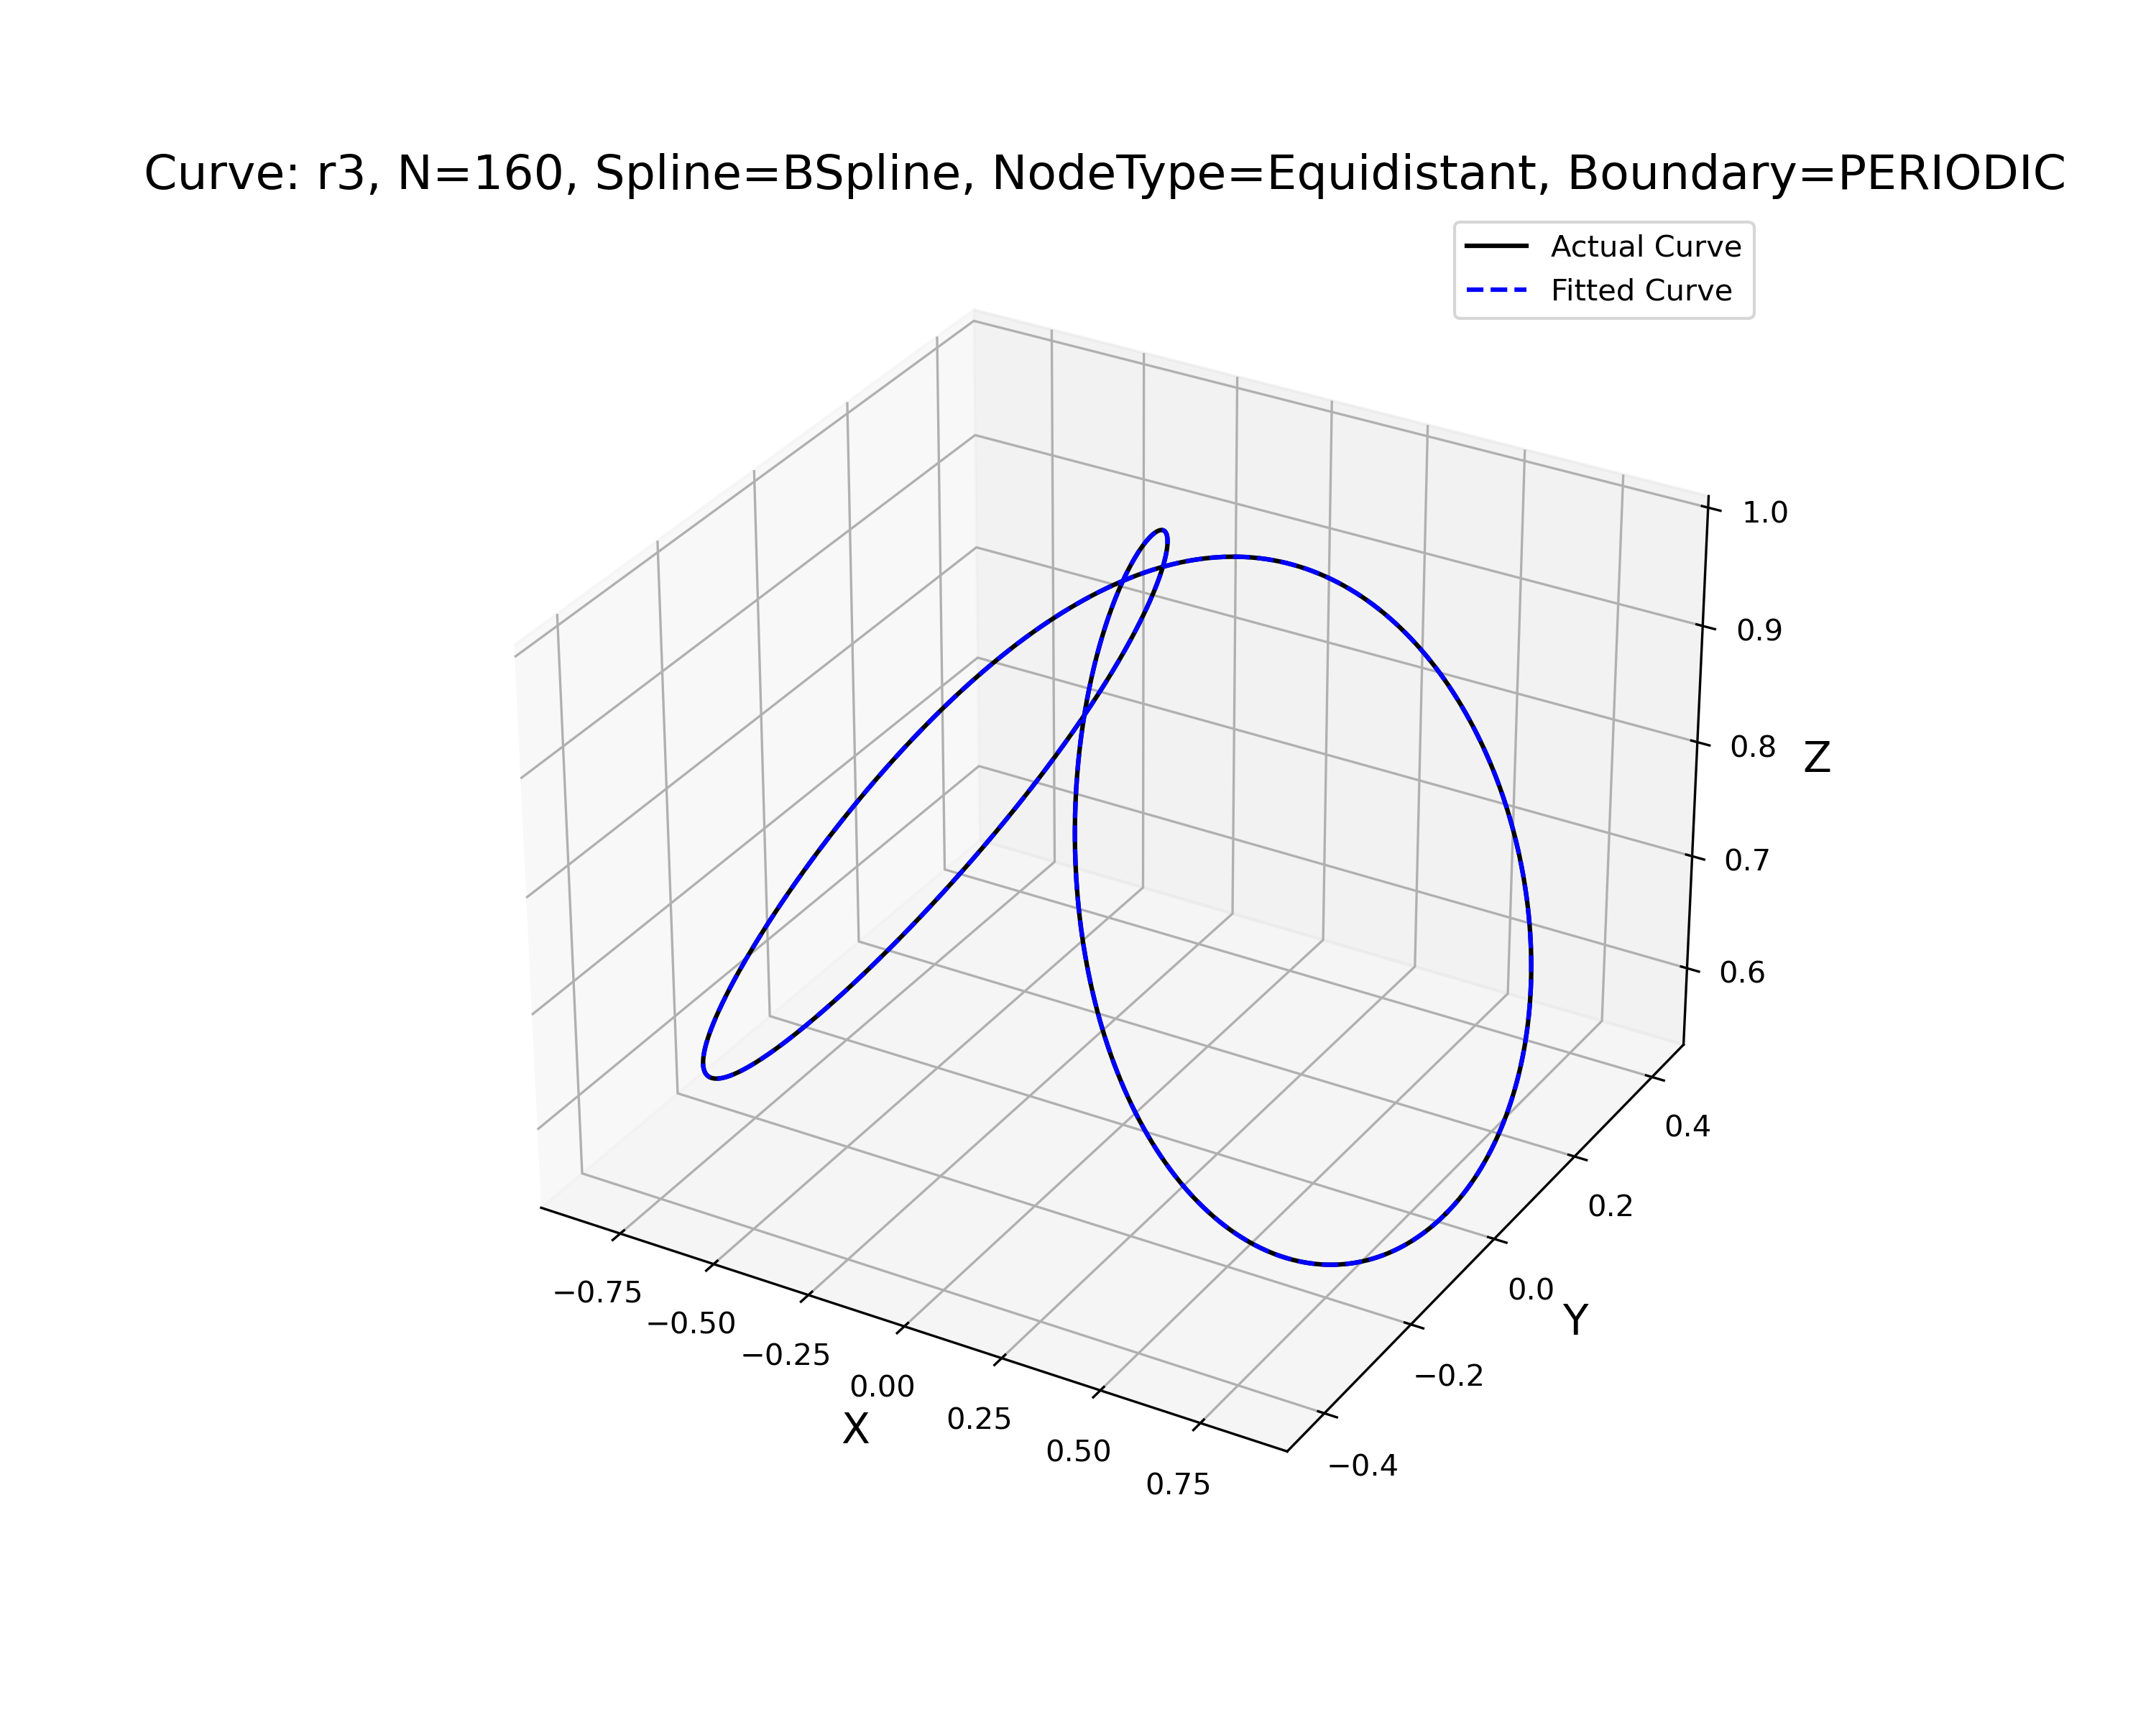
\includegraphics[width=0.45\textwidth]{../figure/problemE/N_160_r3_BSpline_Equidistant_PERIODIC_3D.png} &
    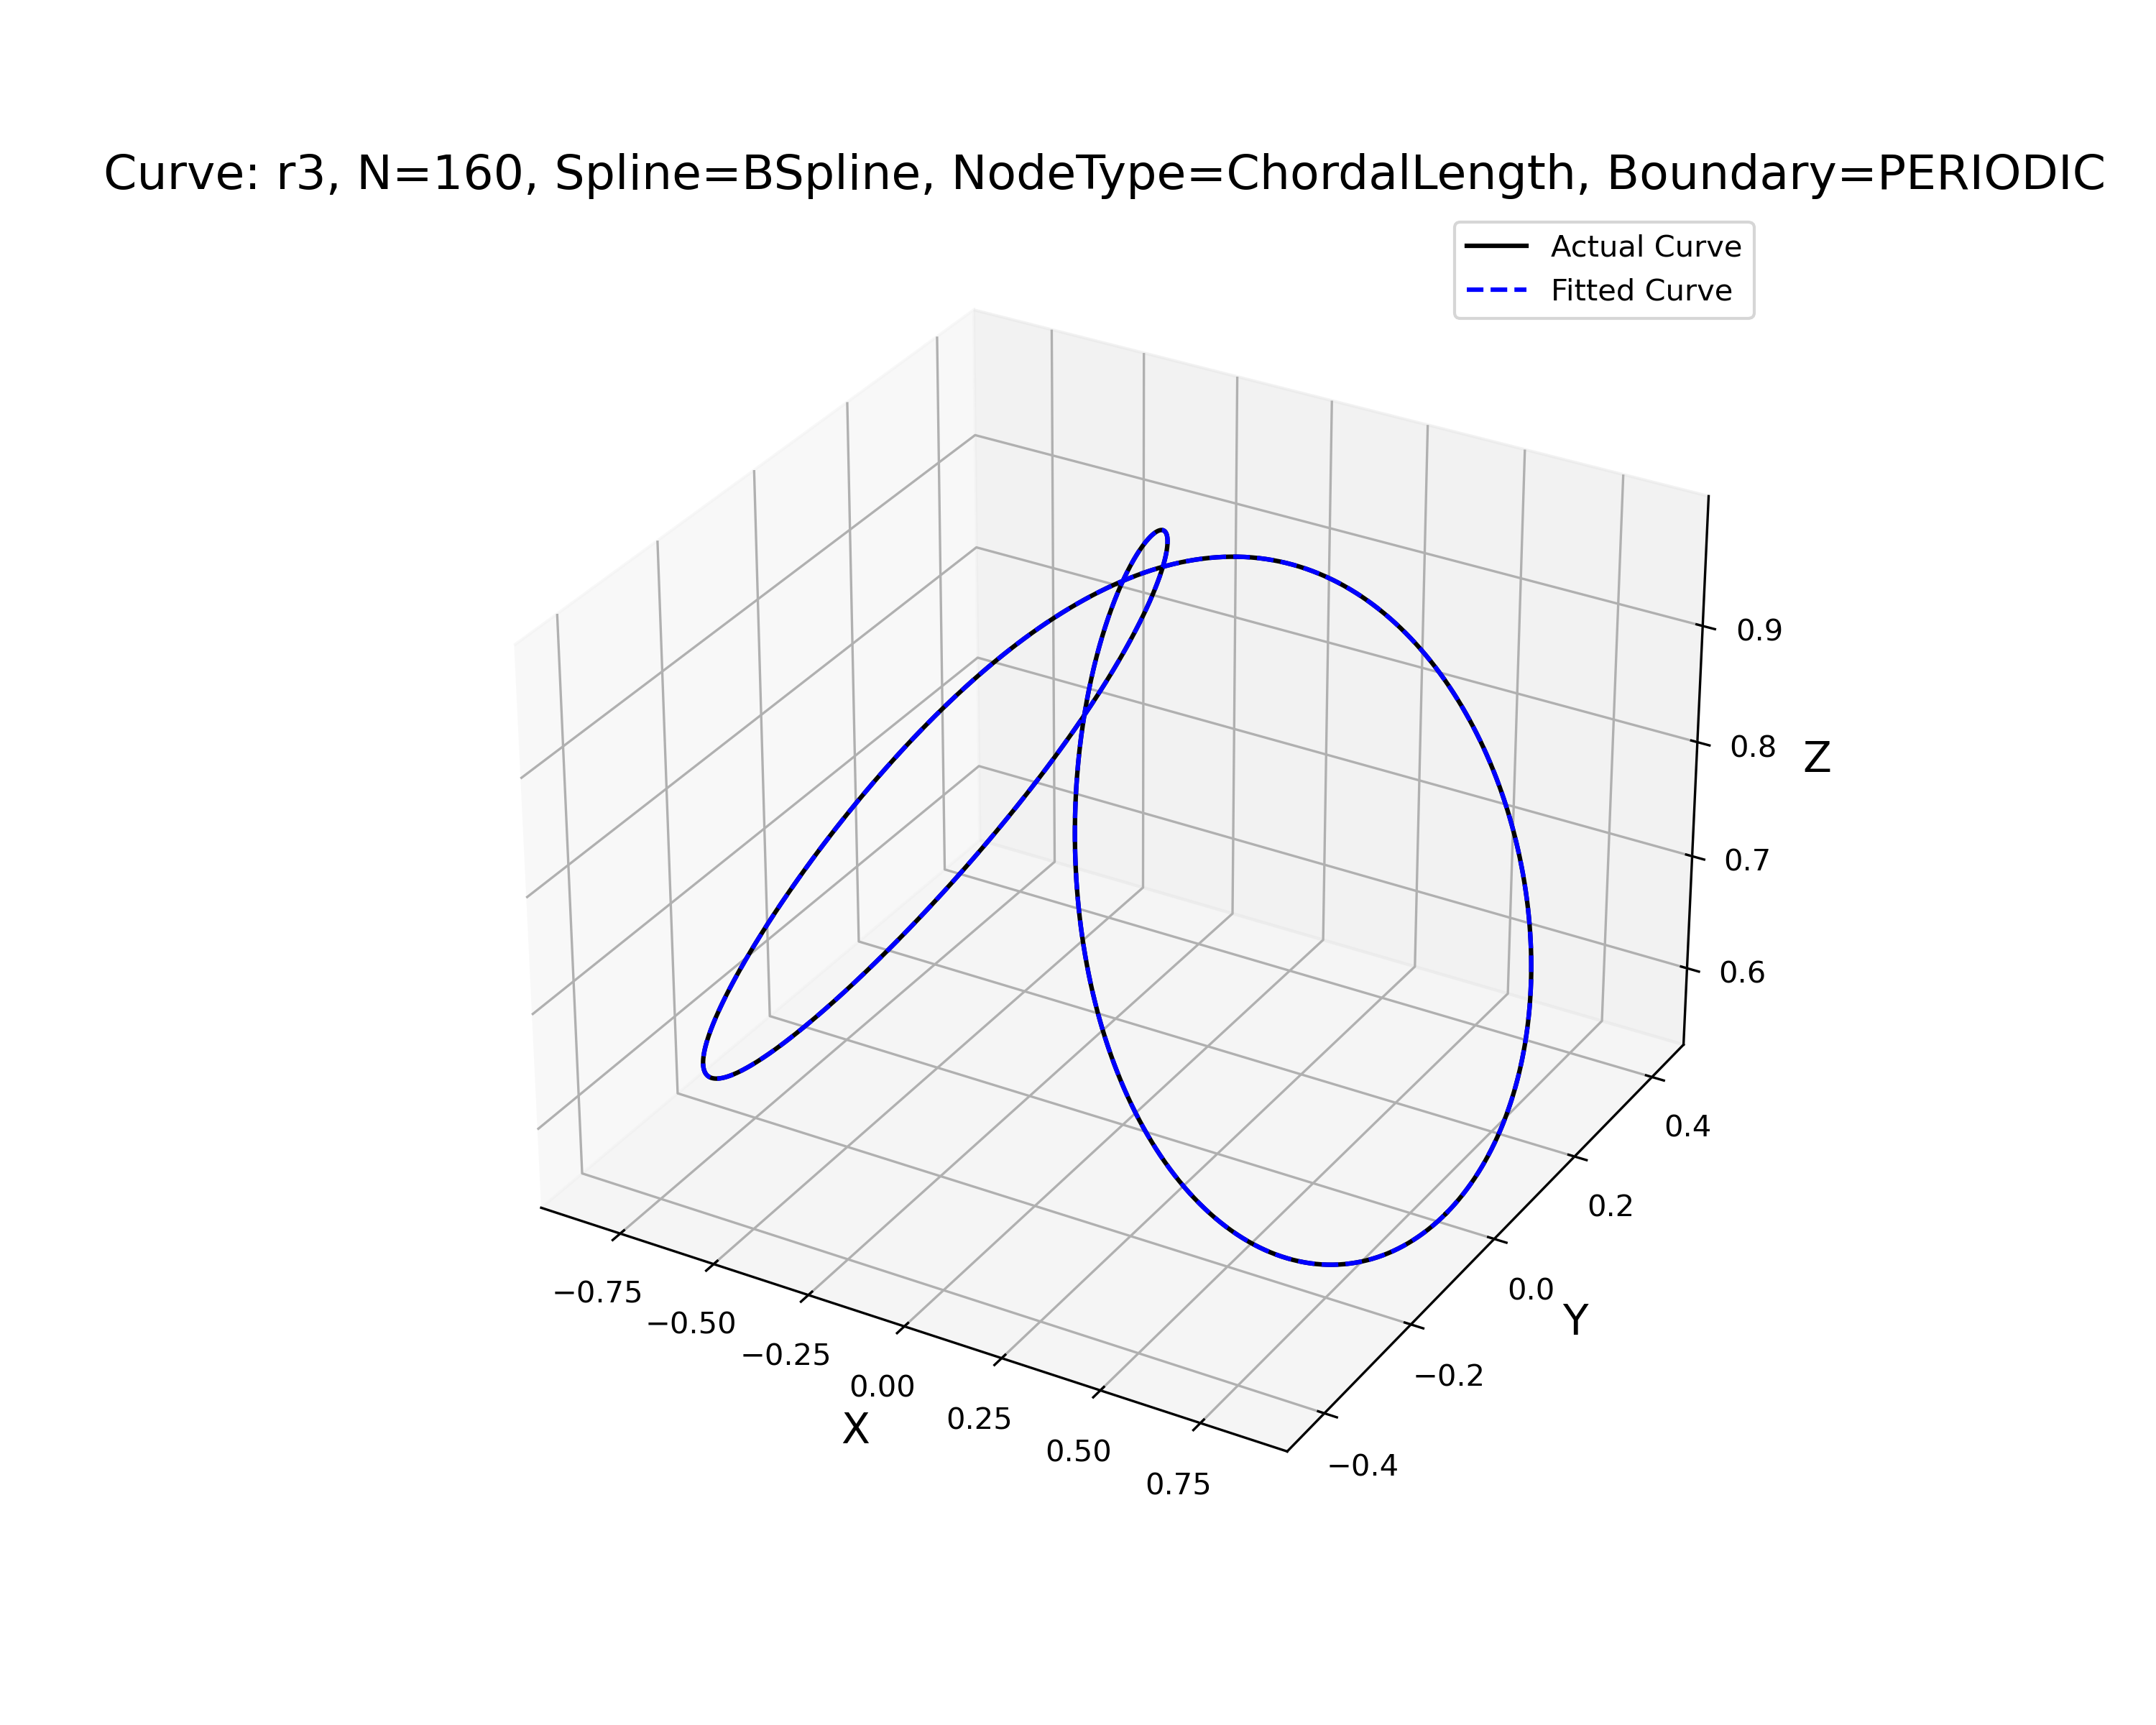
\includegraphics[width=0.45\textwidth]{../figure/problemE/N_160_r3_BSpline_ChordalLength_PERIODIC_3D.png} \\
  \end{tabular}
  \renewcommand{\figurename}{Fig.}
  \caption{Comparison of Equidistant and Chordal Length for curve \(r_3\) with PERIODIC boundary condition}
  \label{fig:r3_nodeType_compare}
\end{figure}

The fitting effect of curve \(r_3\) is shown in
Fig.\ref{fig:r3_nodeType_compare}. This is also a smooth curve without rapid
changes, so both equidistant nodes and cumulative chordal length methods can
achieve good fitting results.

Combining theory and the practical analysis of the cumulative chordal length
method and equidistant nodes method as above, the following conclusions can be
drawn:

\textbf{Cumulative Chordal Length Method}
\begin{itemize}
  \item \textbf{Advantages:}
        \begin{itemize}
          \item Better adapts to the geometric shape of the curve.
          \item Nodes are densely distributed in regions with rapid changes (e.g., curve turns
                or high curvature areas), improving fitting accuracy.
          \item Avoids the "oscillation" phenomenon (Runge phenomenon), especially in
                polynomial interpolation.
        \end{itemize}
  \item \textbf{Disadvantages:}
        \begin{itemize}
          \item Node distribution requires calculating cumulative chord length, increasing
                computational complexity.
          \item Suitable for complex curves but may lead to overly dense distribution for very
                smooth curves.
        \end{itemize}
\end{itemize}

\textbf{Equidistant Nodes Method}
\begin{itemize}
  \item \textbf{Advantages:}
        \begin{itemize}
          \item Simple node distribution, easy to implement.
          \item Provides uniform coverage for smooth curves or regions with small changes.
          \item High computational efficiency, especially suitable for uniformly distributed
                data.
        \end{itemize}
  \item \textbf{Disadvantages:}
        \begin{itemize}
          \item For curves with rapid changes, fitting errors may be significant as rapidly
                changing regions are not sufficiently sampled.
          \item Prone to the "oscillation" phenomenon, especially at the ends of the curve.
        \end{itemize}
\end{itemize}

\section{Problem F}
Compile and run the program \verb|F.cpp|. Its output includes the values of the interpolation curves for plotting. The data stores in the directory \verb|output\problemF|.
It will also run the program \verb|plotF_trunc.py| and \verb|plotF_divide.py| to plot the truncated power function and divided truncated power function. The figures are stored in the directory \verb|figure\problemF|.

First, the calculation and plotting of the first-order truncated power function
were tested, as shown in Fig.\ref{fig:trunc_power_1}.
\begin{figure}[H]
  \centering
  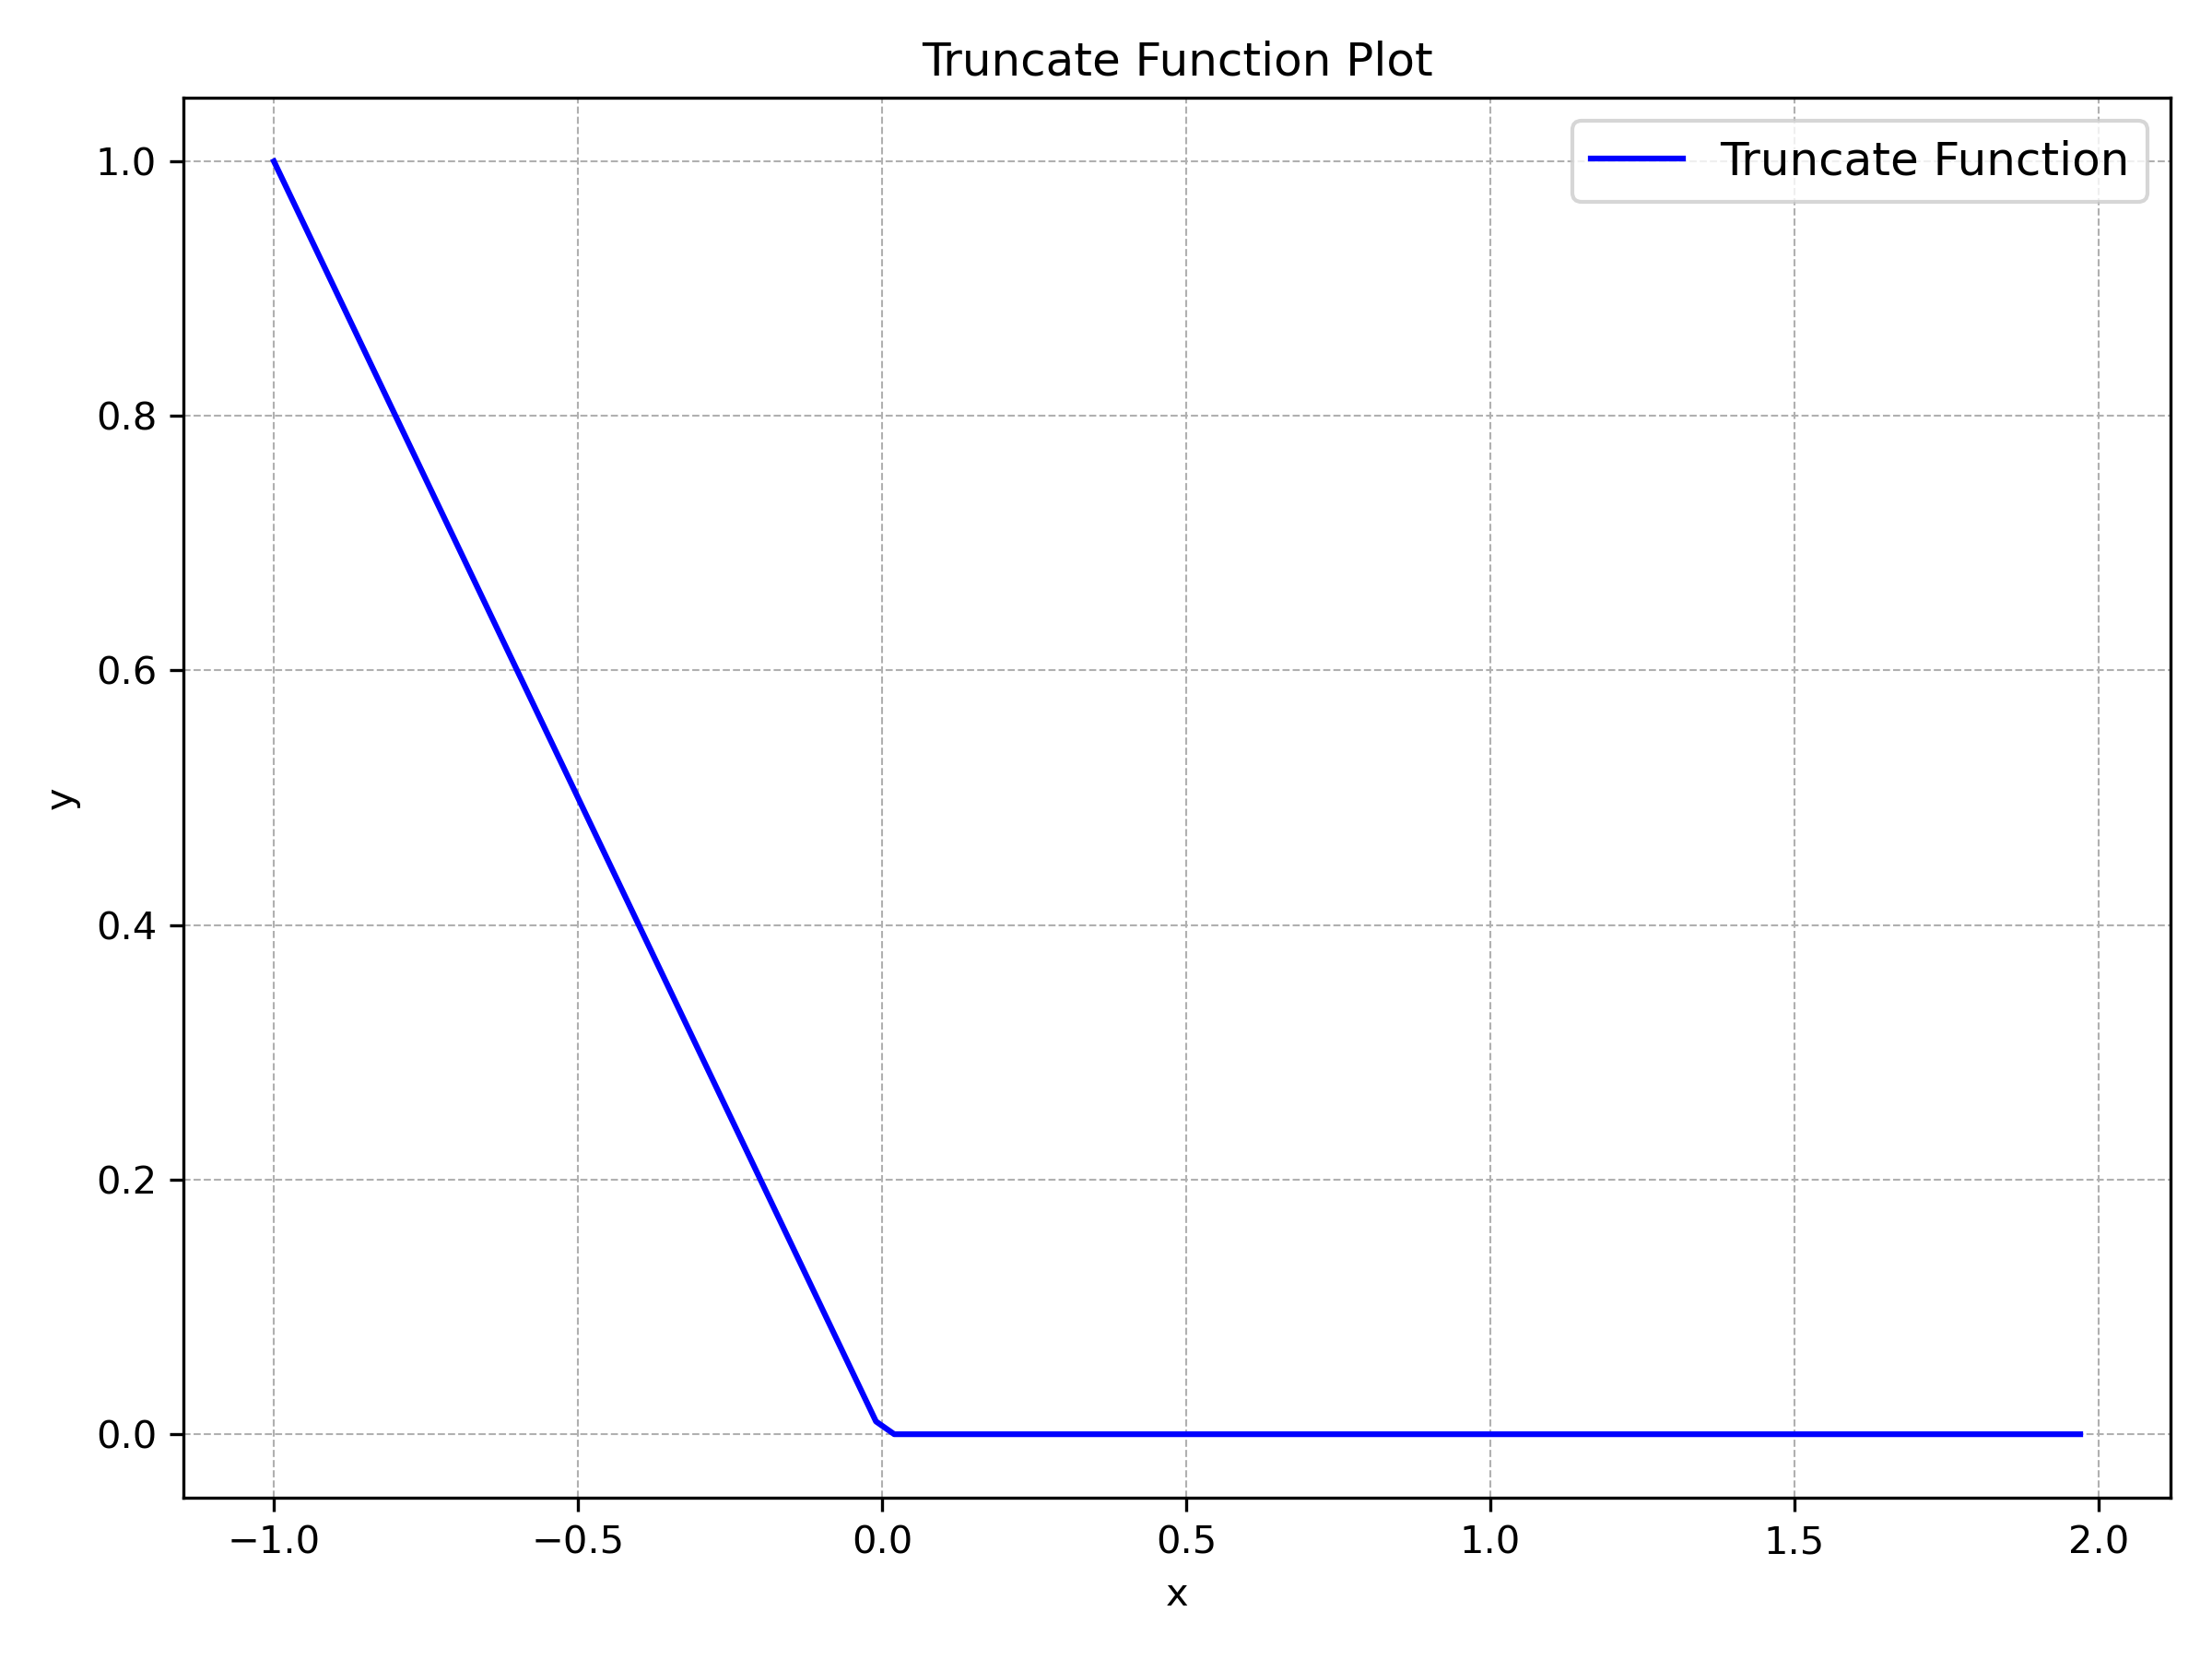
\includegraphics[width=0.6\textwidth]{../figure/problemF/trunc_1.png}
  \renewcommand{\figurename}{Fig.}
  \caption{Calculation and plotting of the first-order truncated power function}
  \label{fig:trunc_power_1}
\end{figure}

Next, the calculation and plotting of the second-order truncated power function
were tested, as shown in Fig.\ref{fig:trunc_power_2}.
\begin{figure}[H]
  \centering
  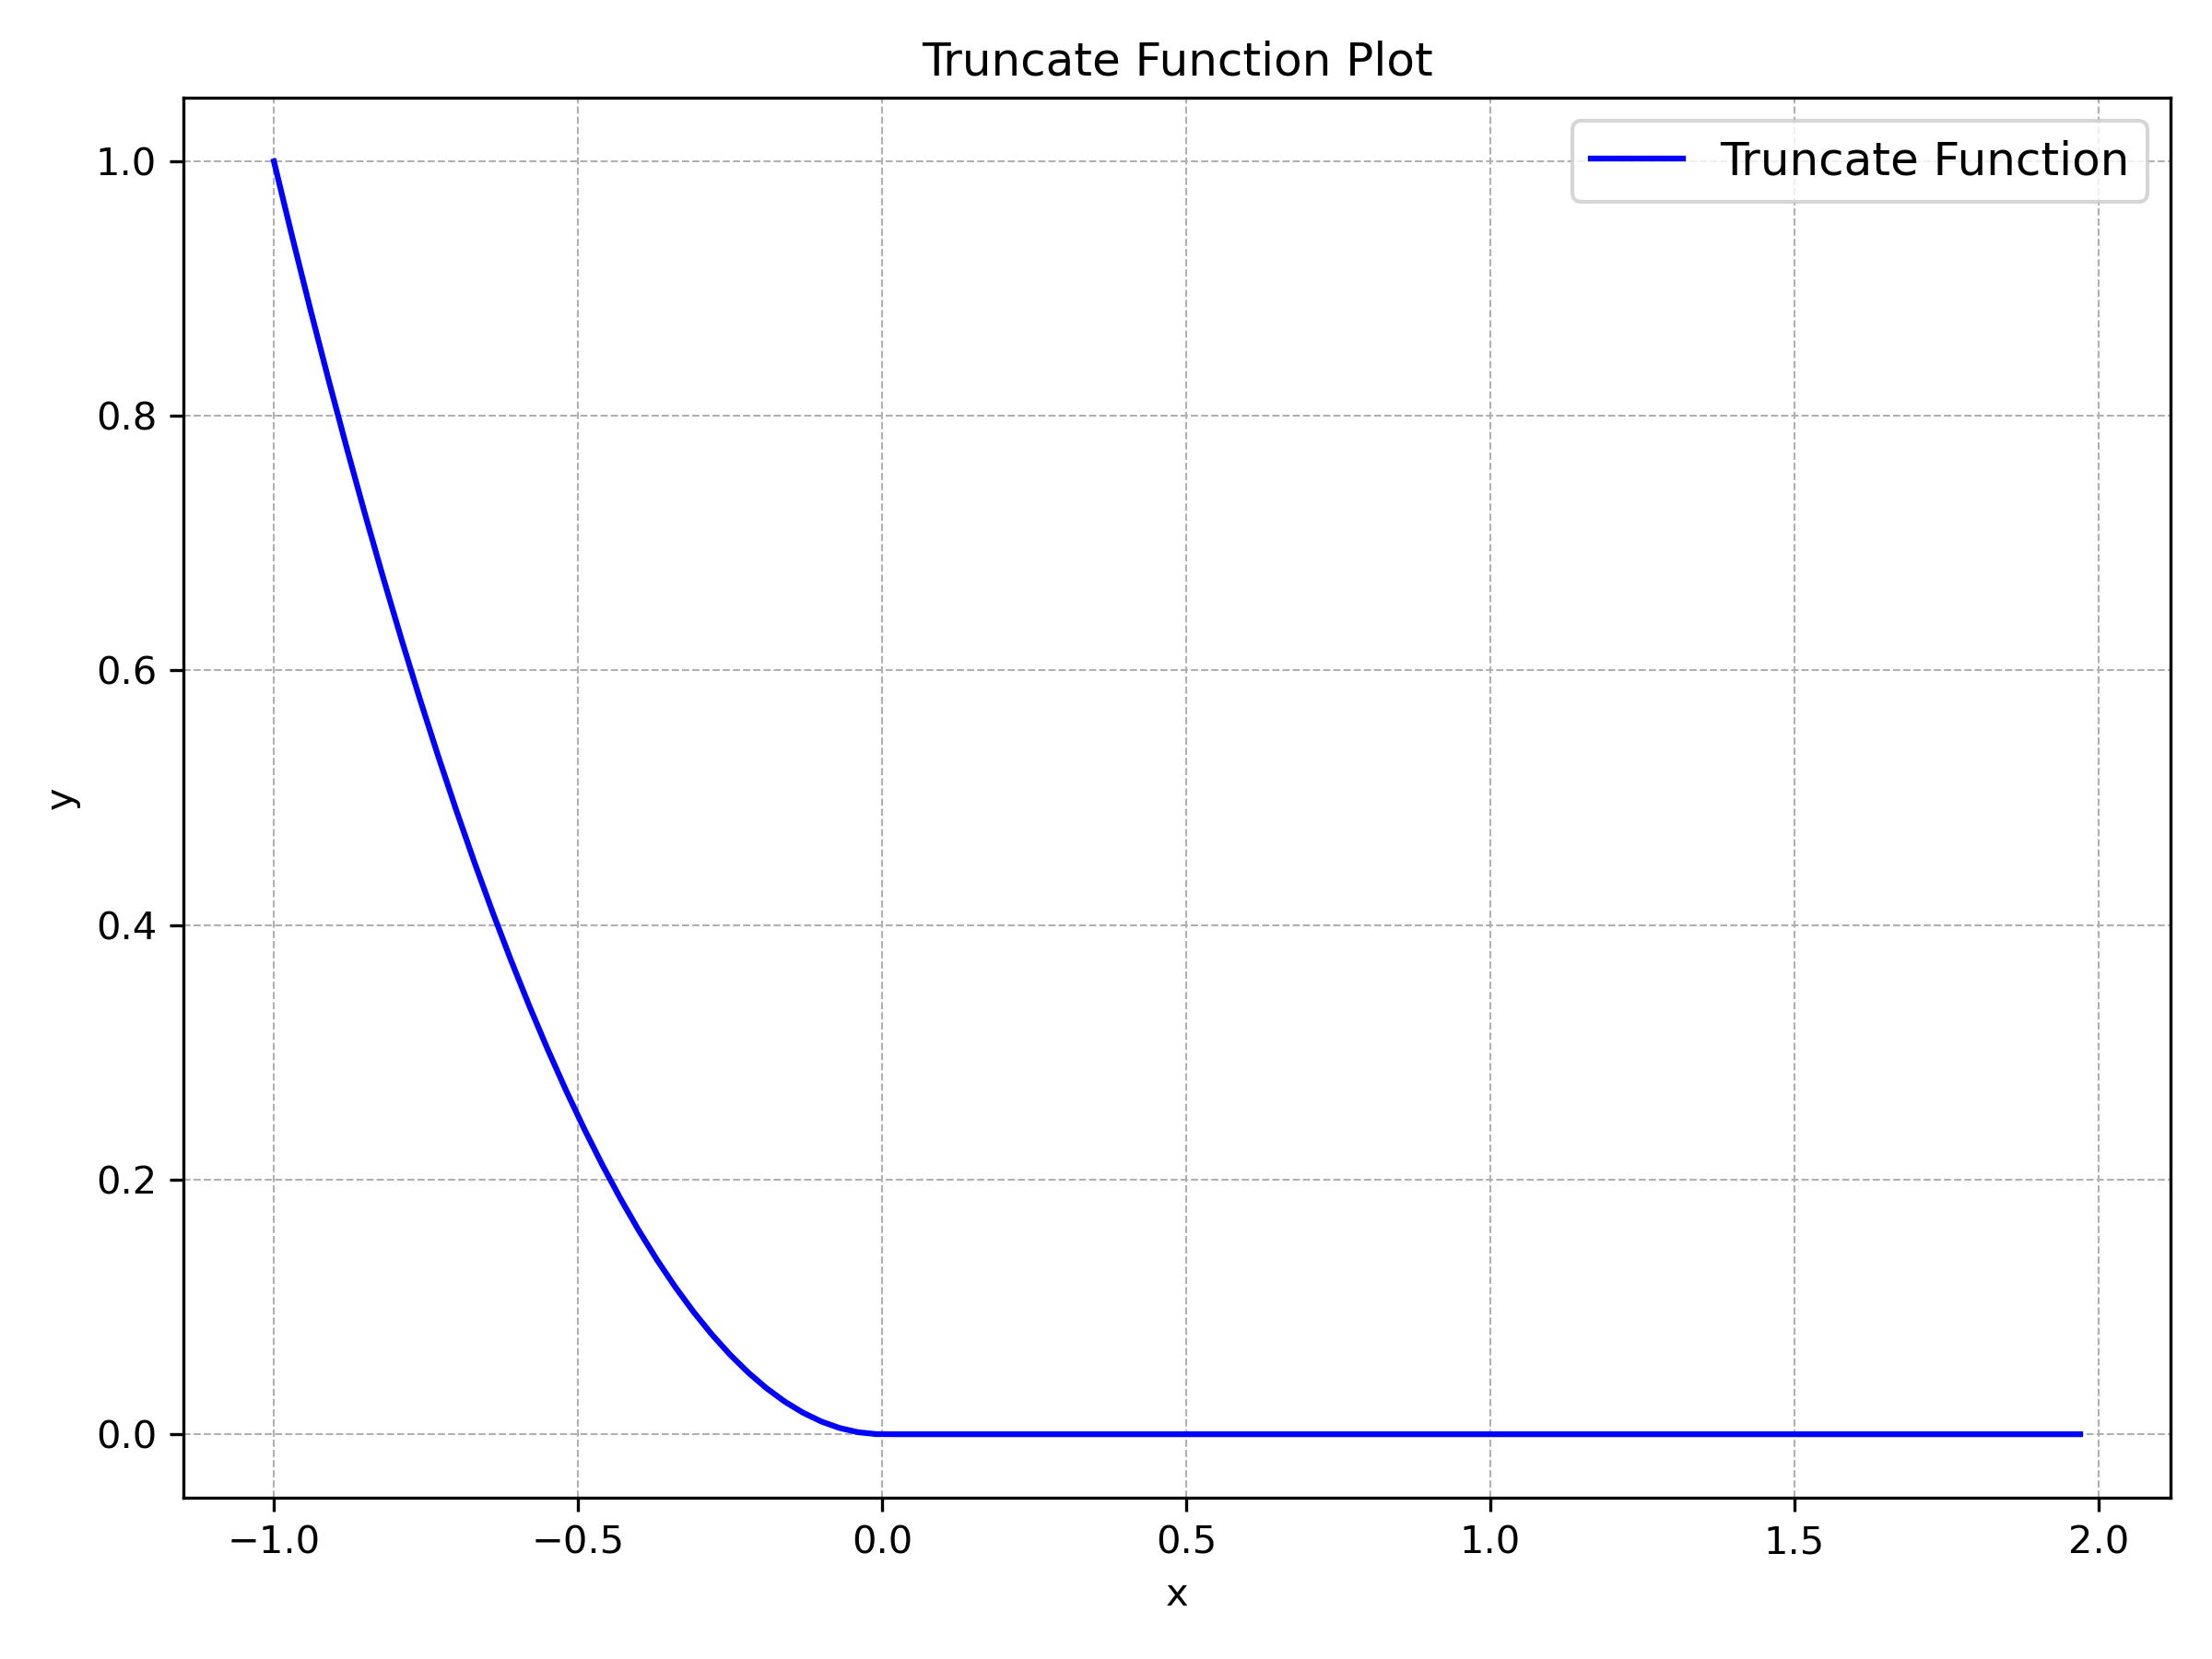
\includegraphics[width=0.6\textwidth]{../figure/problemF/trunc_2.png}
  \renewcommand{\figurename}{Fig.}
  \caption{Calculation and plotting of the second-order truncated power function}
  \label{fig:trunc_power_2}
\end{figure}

Additionally, the difference calculation and plotting of the first-order
truncated power function were tested, as shown in
Fig.\ref{fig:divided_trunc_power_1}.
\begin{figure}[H]
  \centering
  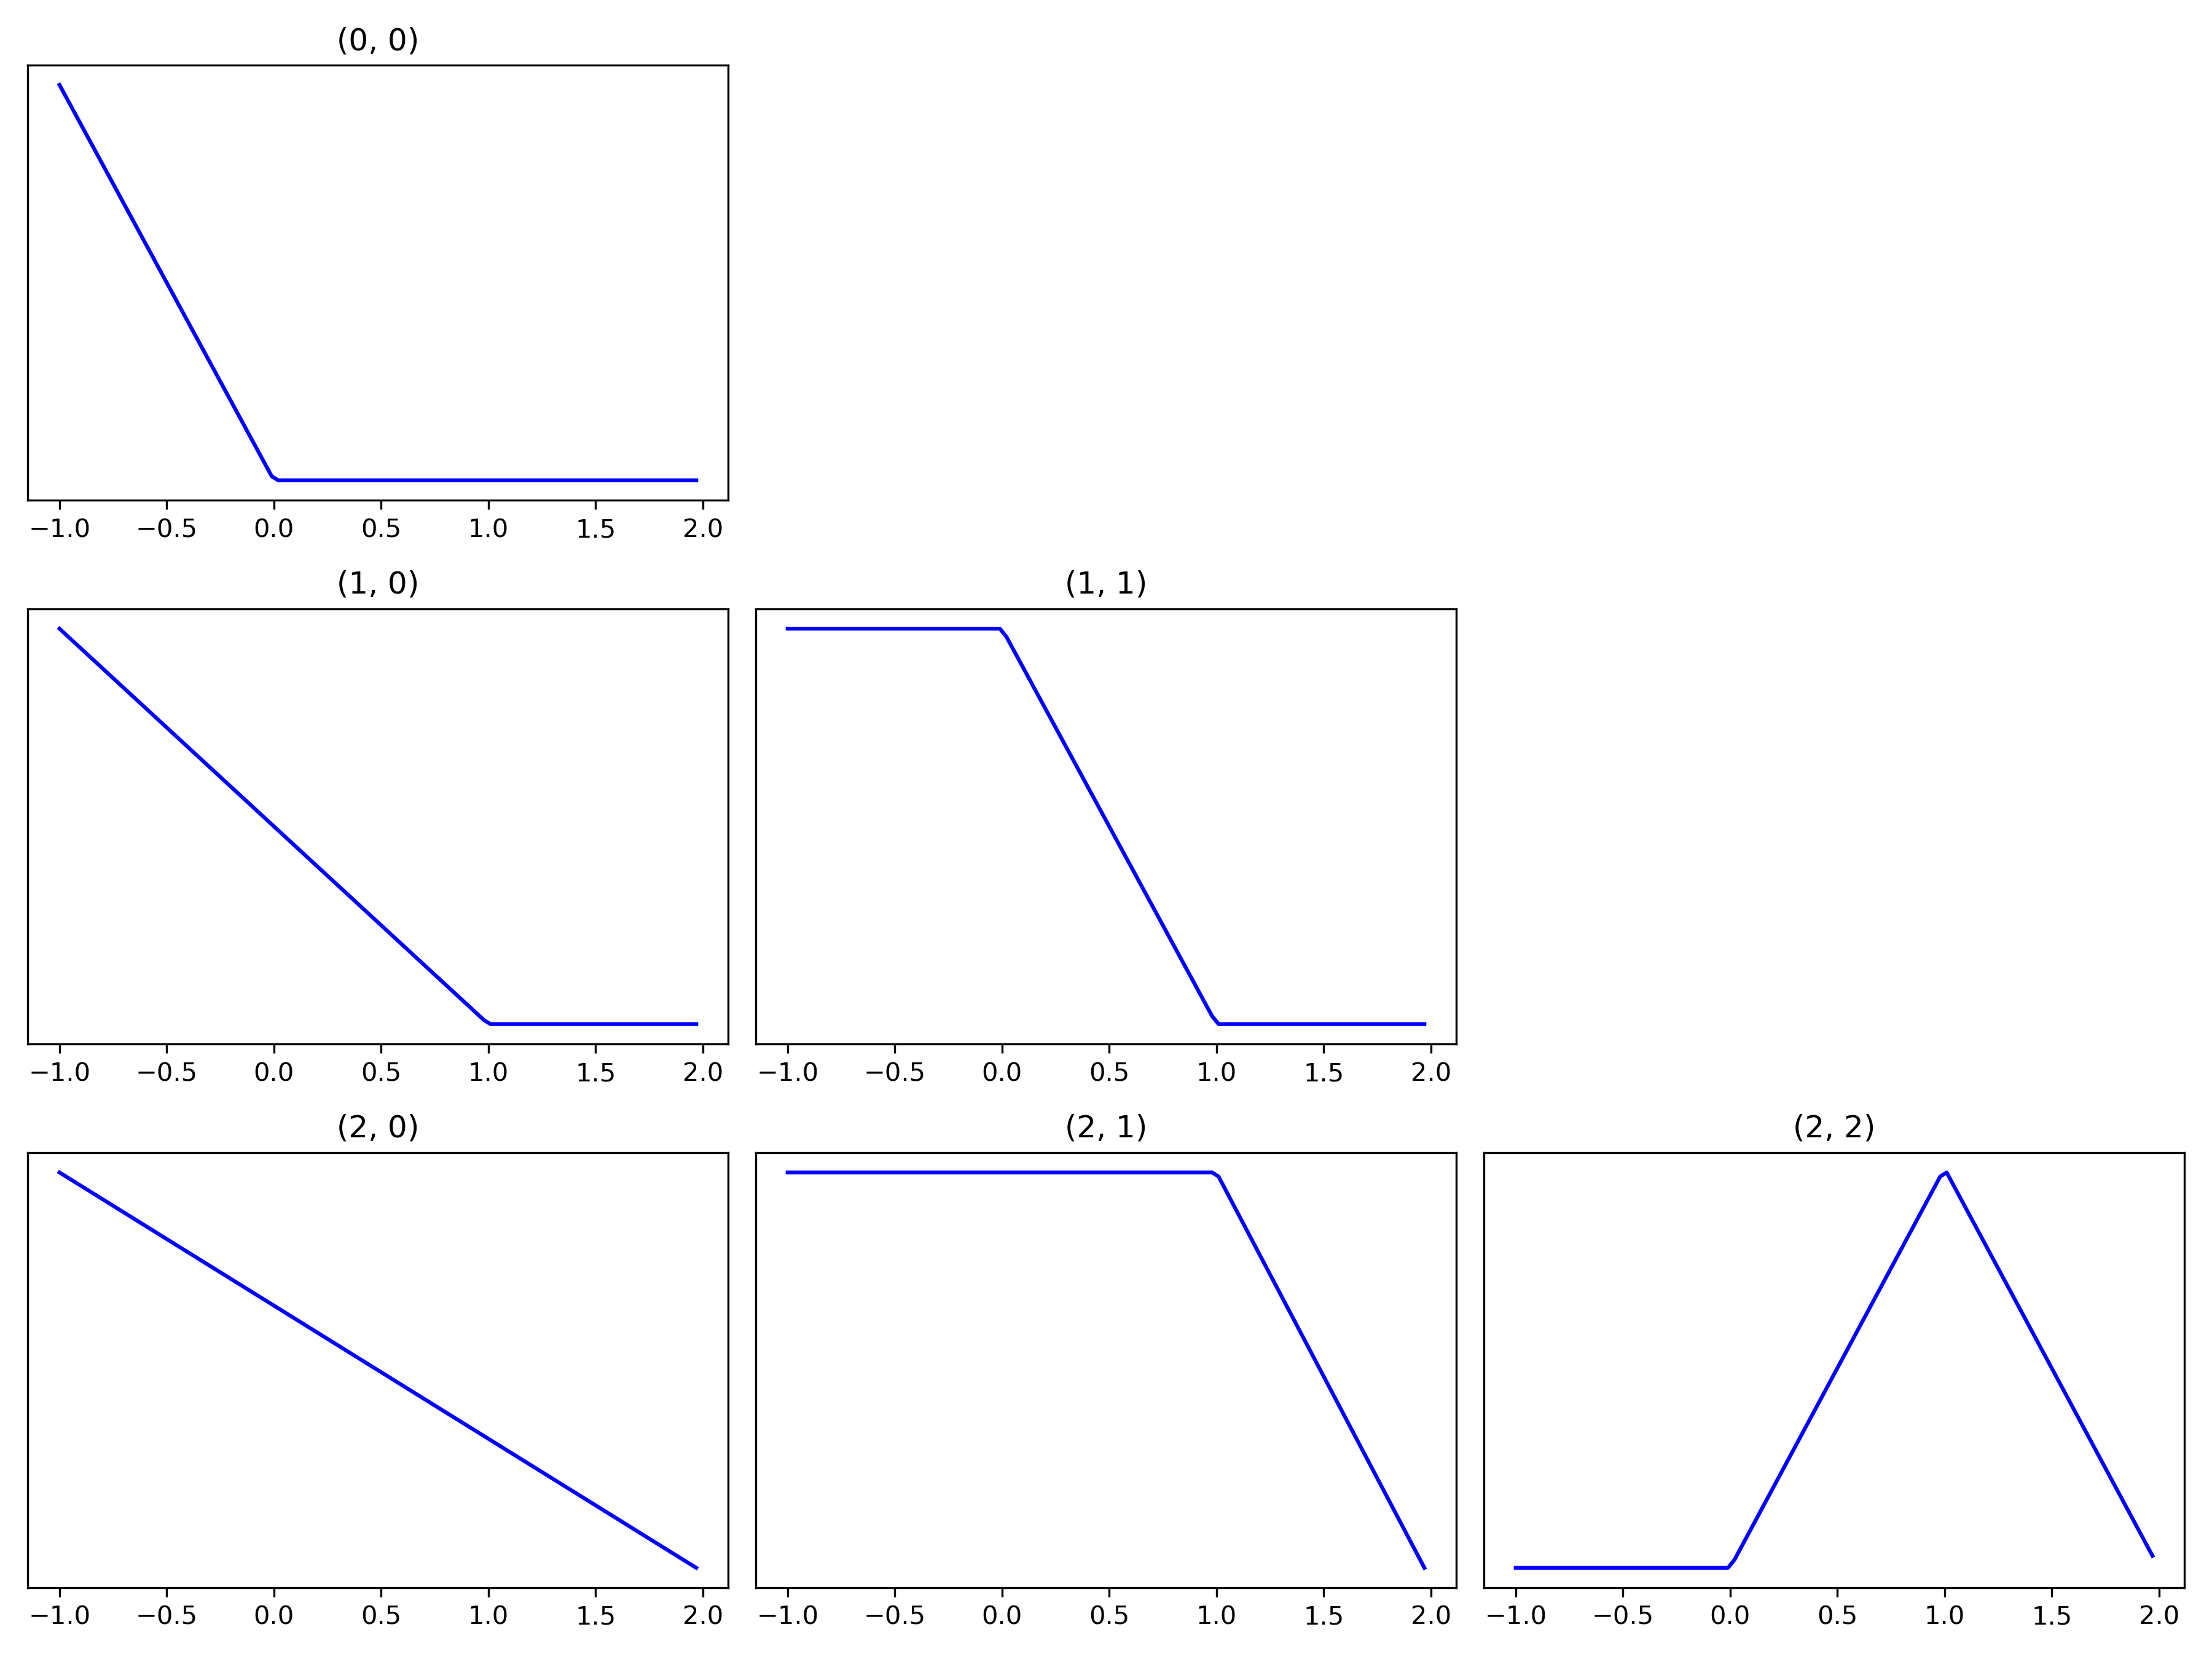
\includegraphics[width=0.6\textwidth]{../figure/problemF/divided_1.png}
  \renewcommand{\figurename}{Fig.}
  \caption{Difference matrix calculation of the first-order truncated power function}
  \label{fig:divided_trunc_power_1}
\end{figure}

Finally, the difference calculation and plotting of the second-order truncated
power function were tested, as shown in Fig.\ref{fig:divided_trunc_power_2}.
\begin{figure}[H]
  \centering
  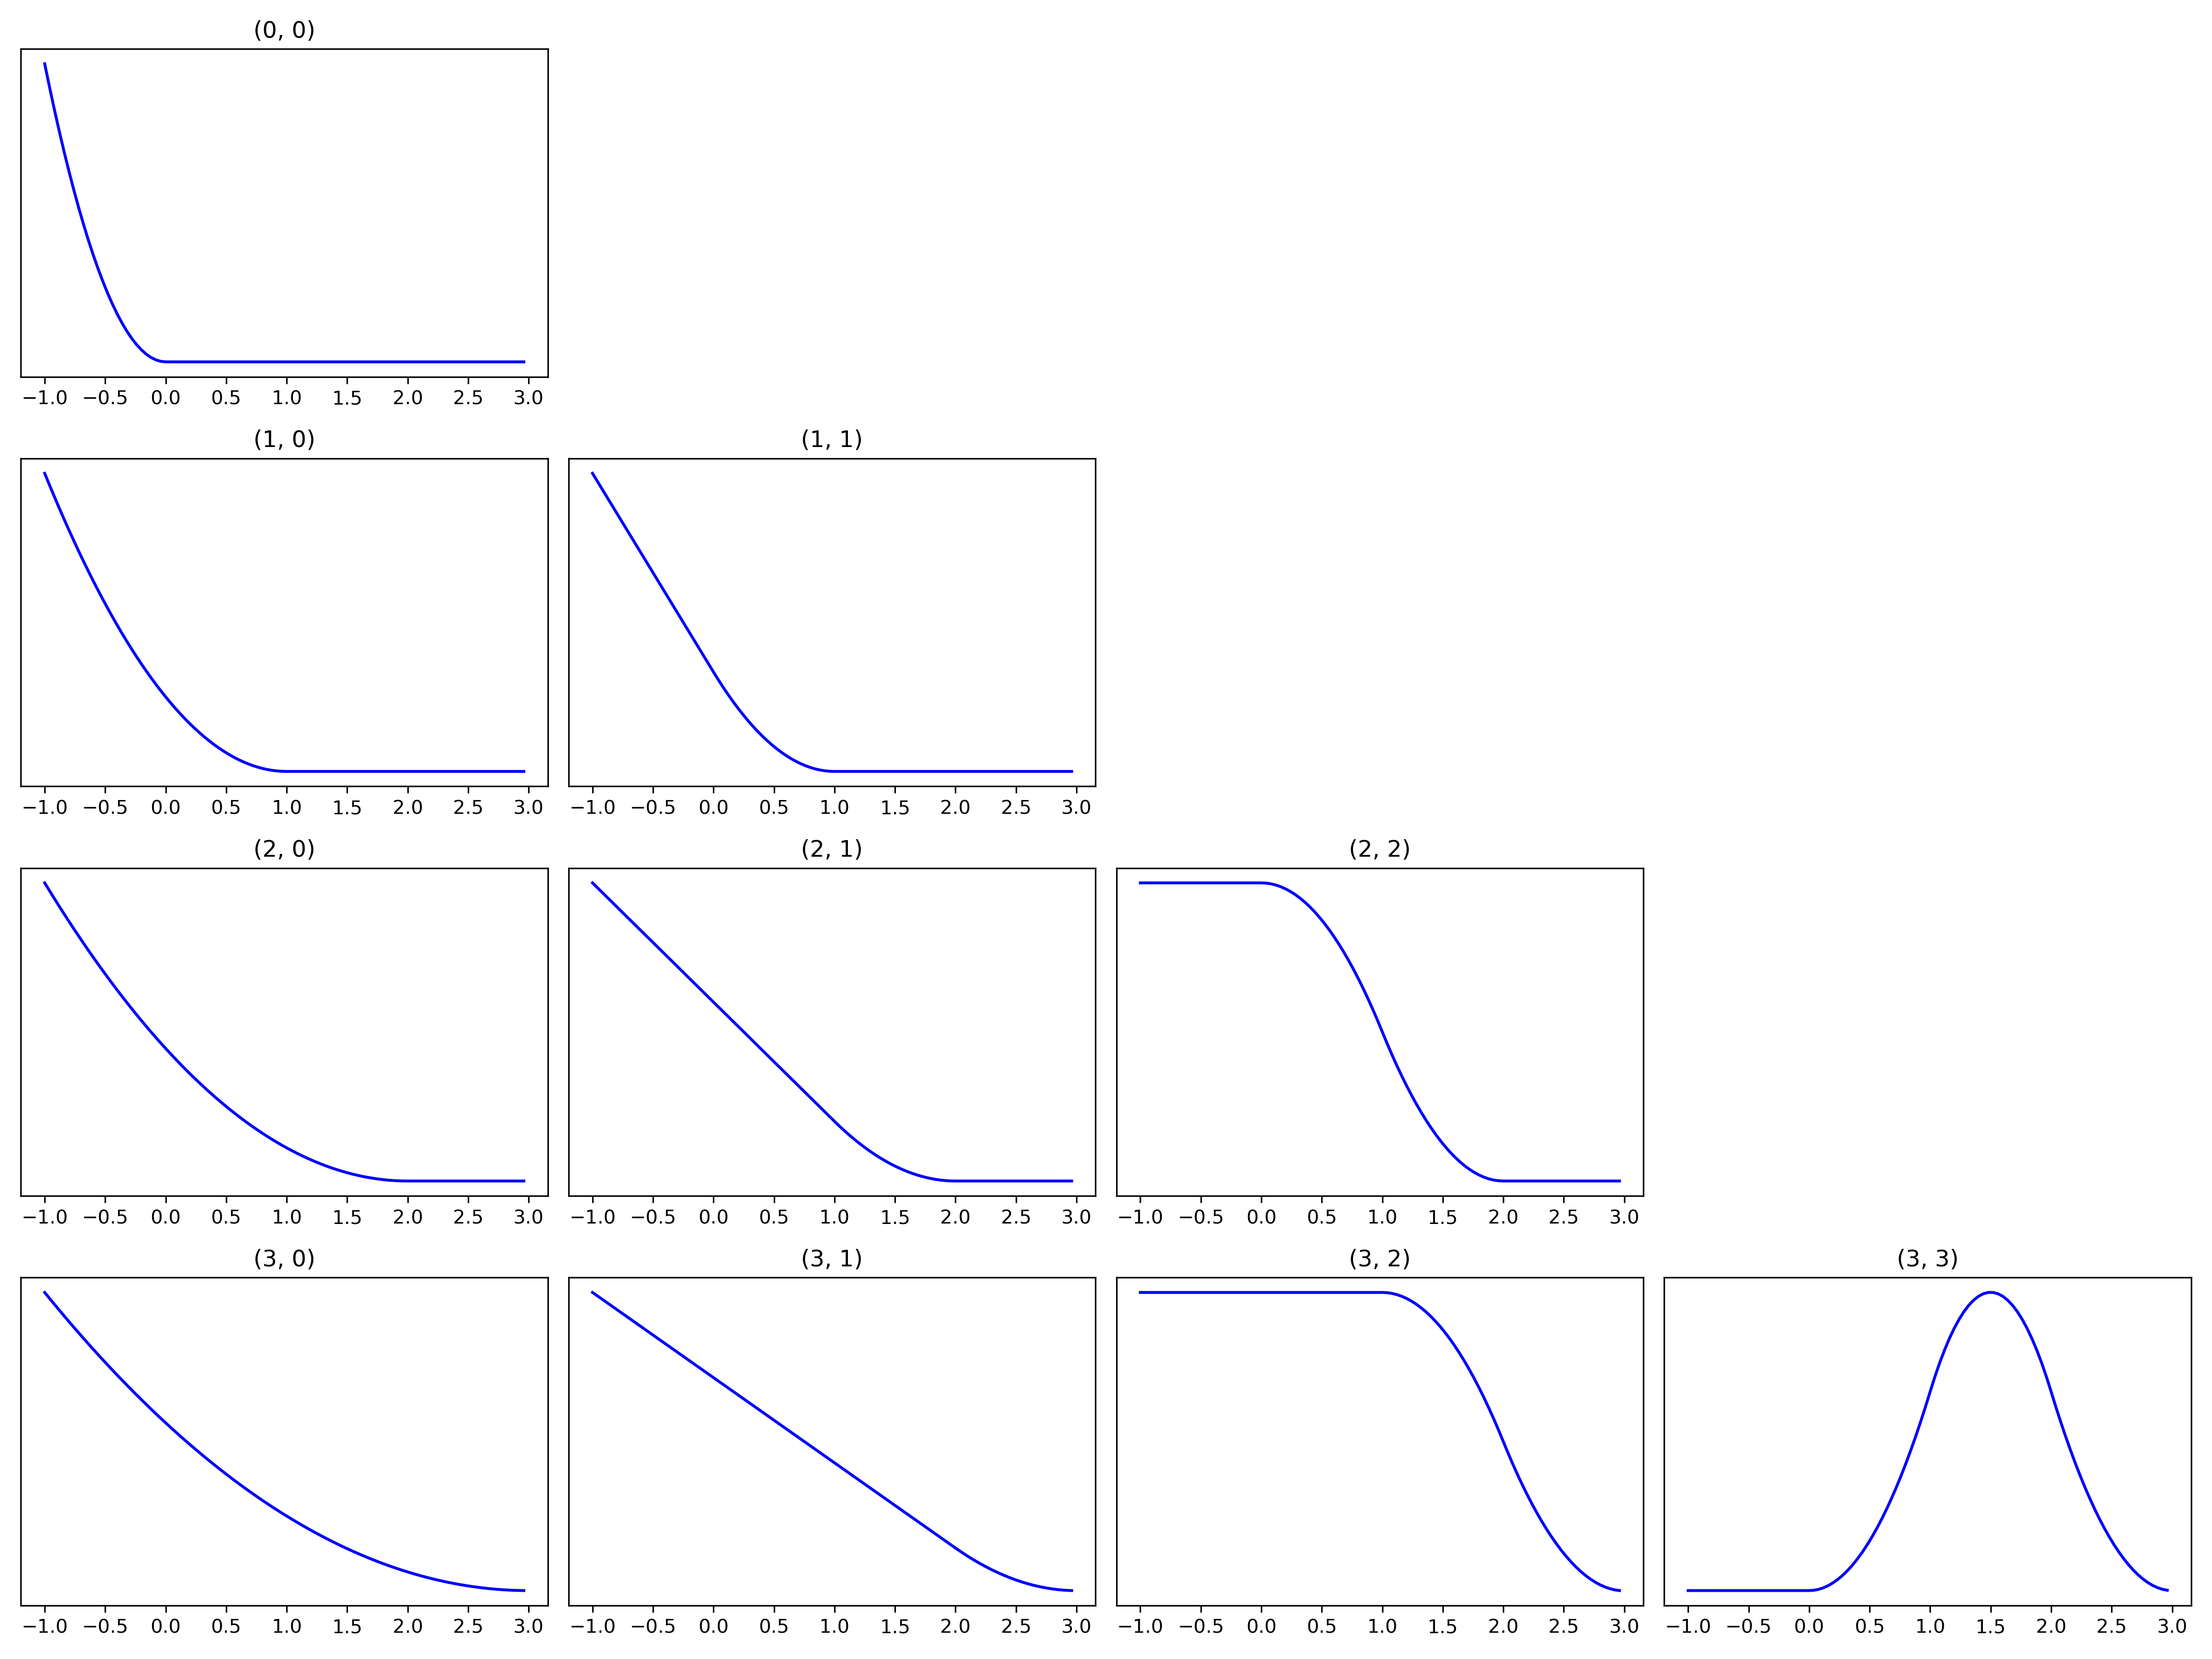
\includegraphics[width=0.8\textwidth]{../figure/problemF/divided_2.png}
  \renewcommand{\figurename}{Fig.}
  \caption{Difference calculation of the second-order truncated power function}
  \label{fig:divided_trunc_power_2}
\end{figure}

\section{Requirement 5}
Compile and run the program \verb|require5.cpp|. Its output includes the coordinate data of the fitted curves to be plotted. The data is stored in the directory \verb|output\requirement5|.

Compile and run the program \verb|plotRequire5.py| to plot the interpolation
curves. The figures are stored in the directory \verb|figure\requirement5|.

Using a third-order B-spline, the input data is:
\begin{verbatim}
std::vector<double> knots = {0, 1, 2, 3, 4, 5, 6};
std::vector<double> coefficients = {0, 1, 0, -1, 0, 1, 0, -1, 0};
\end{verbatim}

Using a fifth-order B-spline, the input data is:
\begin{verbatim}
std::vector<double> knots = {0, 1, 2, 3, 4};
std::vector<double> coefficients = {0, 2, 3, 2, 0, -1, 2, 3, 2};
\end{verbatim}

As shown in Fig.\ref{fig:require5_bspline_curves}, the third-order and
fifth-order B-spline curves are plotted respectively.

\begin{figure}[H]
  \centering
  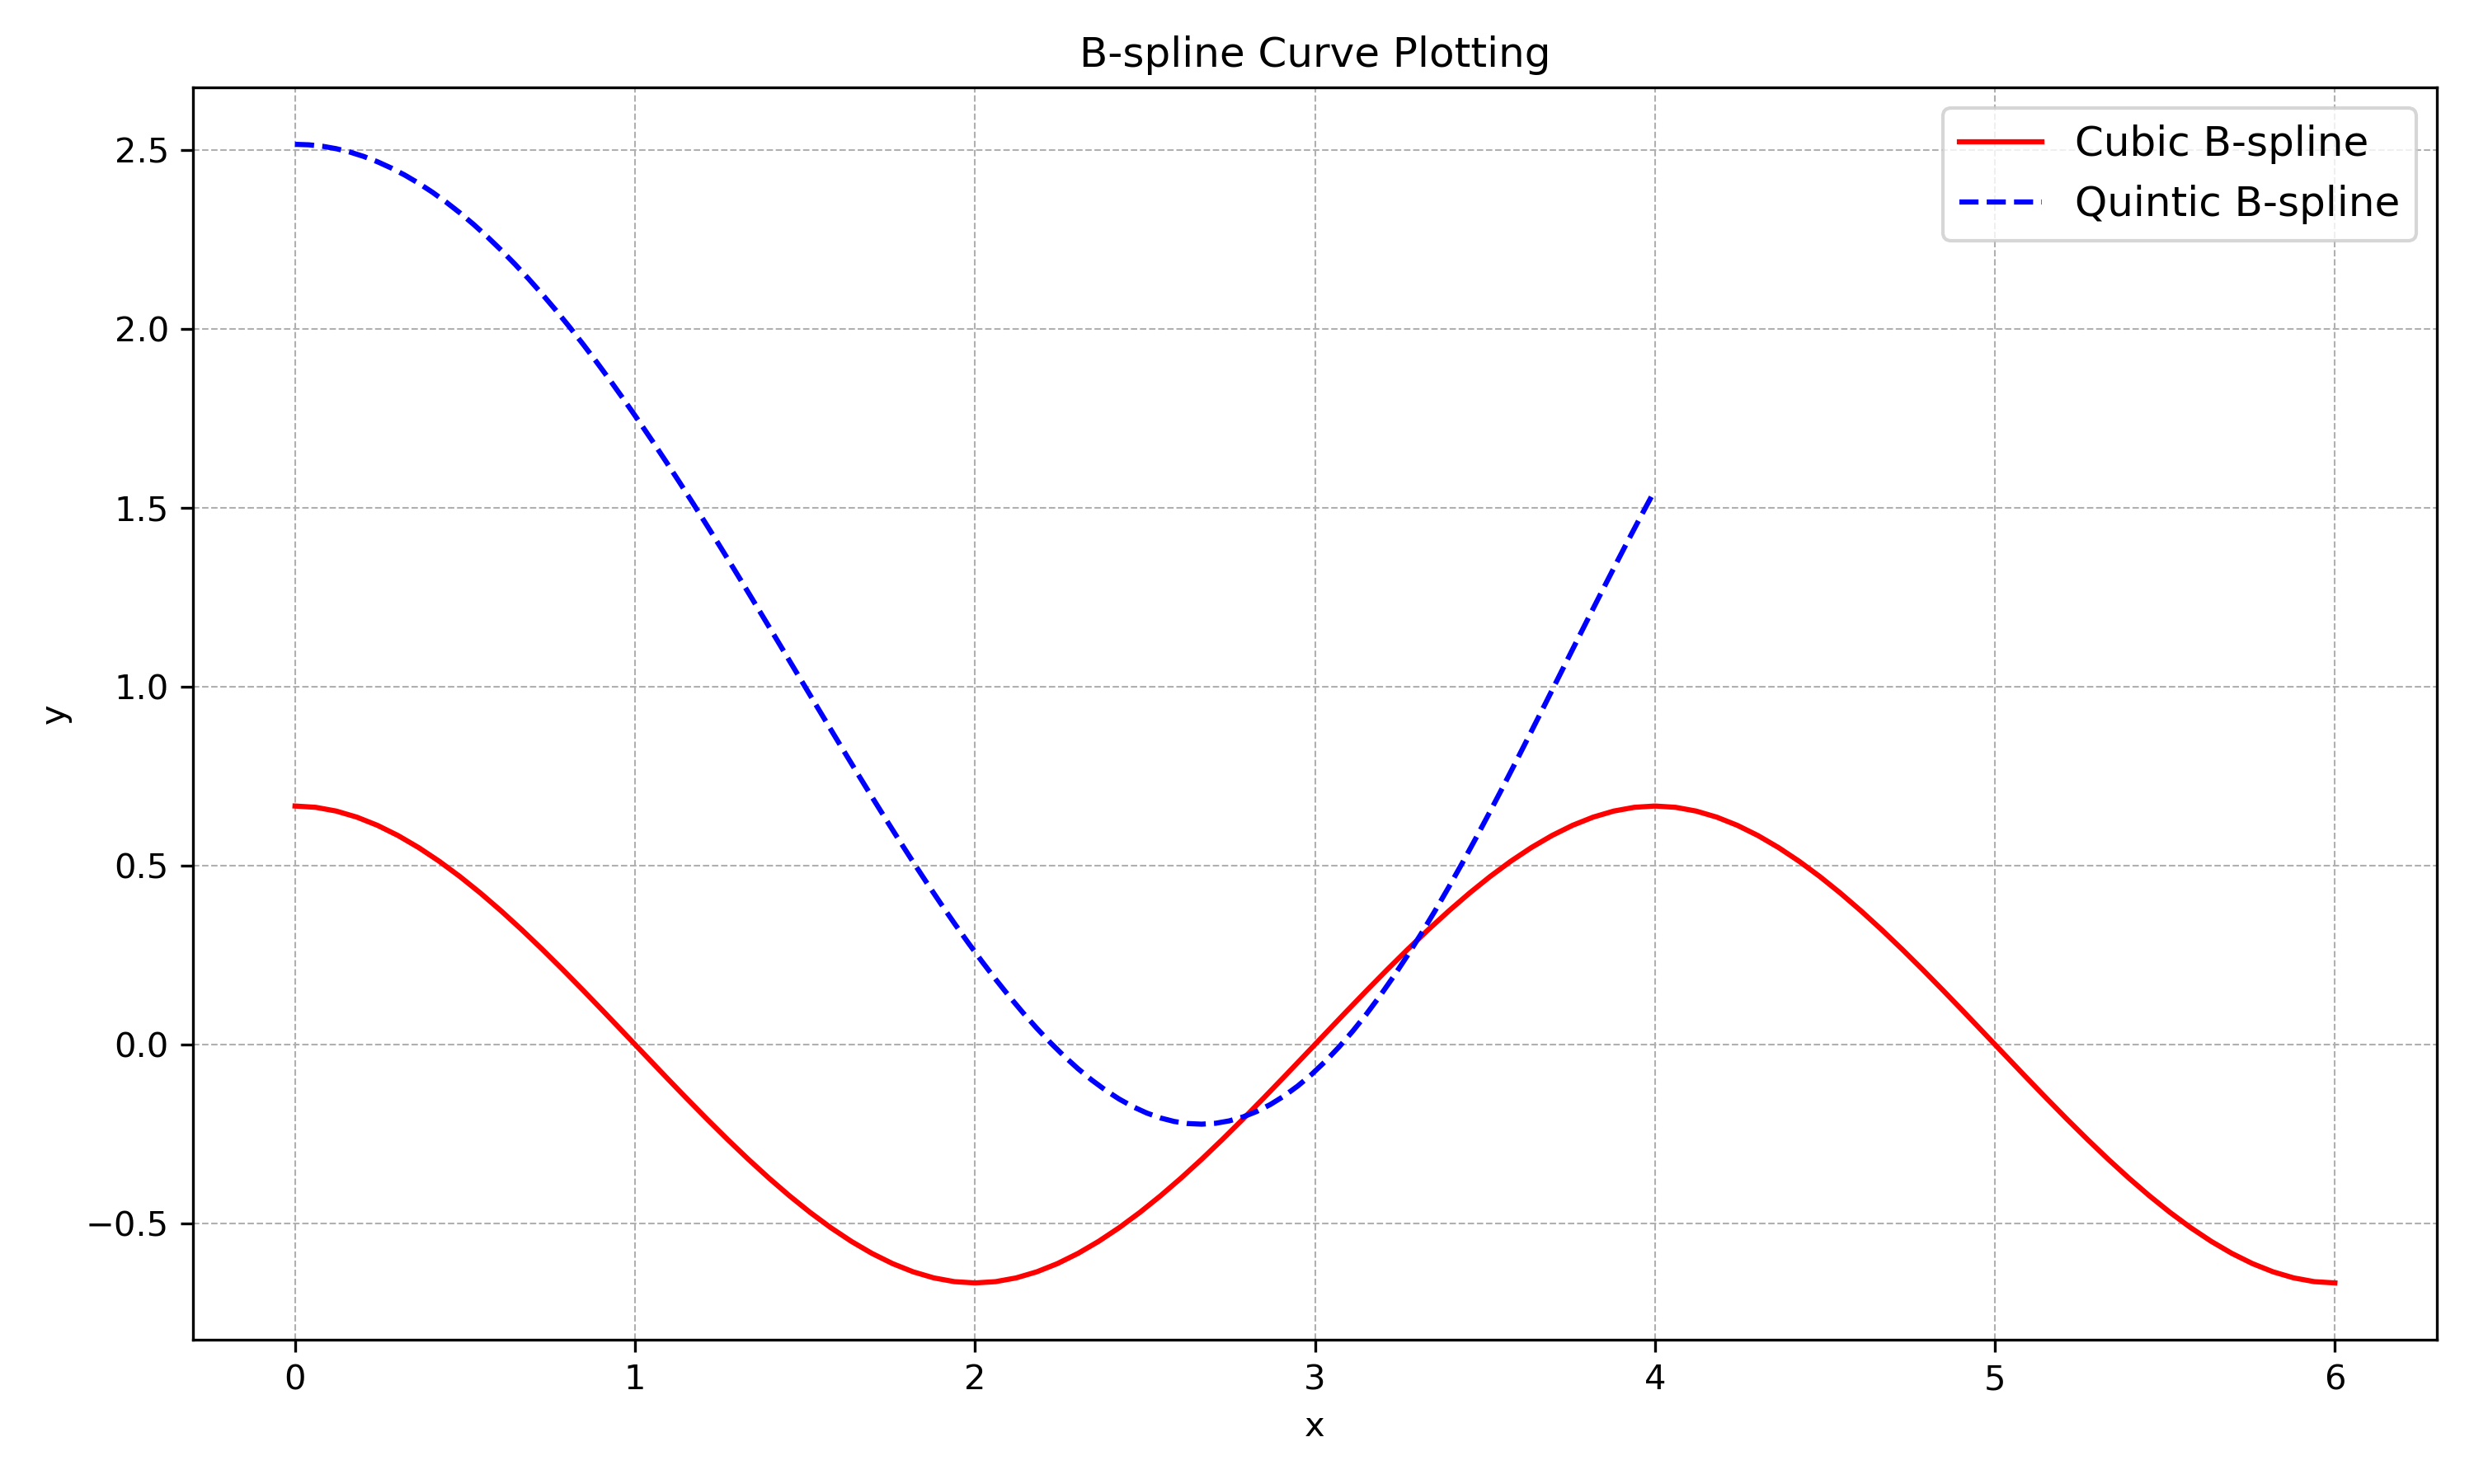
\includegraphics[width=0.8\textwidth]{../figure/requirement5/bspline_curves.png}
  \renewcommand{\figurename}{Fig.}
  \caption{B-spline curves for Requirement 5}
  \label{fig:require5_bspline_curves}
\end{figure}

Therefore, given the dimension and coefficients and knot sequences,
\verb|Bspline.hpp| can implement the plotting of splines of any order and any
nodes.

\section{Test}
Compile and run the program \verb|test.cpp|. Its output includes the max errors and convergence rate of different situations and the values of the interpolation curves for plotting. The data stores in the directory \verb|output\test|.
Run the program \verb|plotTest.py| to plot the interpolation curves and the original function. The figures are stored in the directory \verb|figure/test|.

The program is designed to test first-order B-spline and PPForm interpolation under non-uniform nodes, as well as third-order B-spline and PPForm interpolation under five different boundary conditions, along with their interpolation effects. The target function is $\sin x$, and the interval is $[0,2\pi]$. The program actually uses a quadratic distribution to generate non-uniform nodes.

As shown in Fig.\ref{fig:test_linear}, below are the interpolation results of linear PPForm and BSpline interpolation for different values of \(N\).

\begin{figure}[H]
  \centering
  \begin{tabular}{cc}
    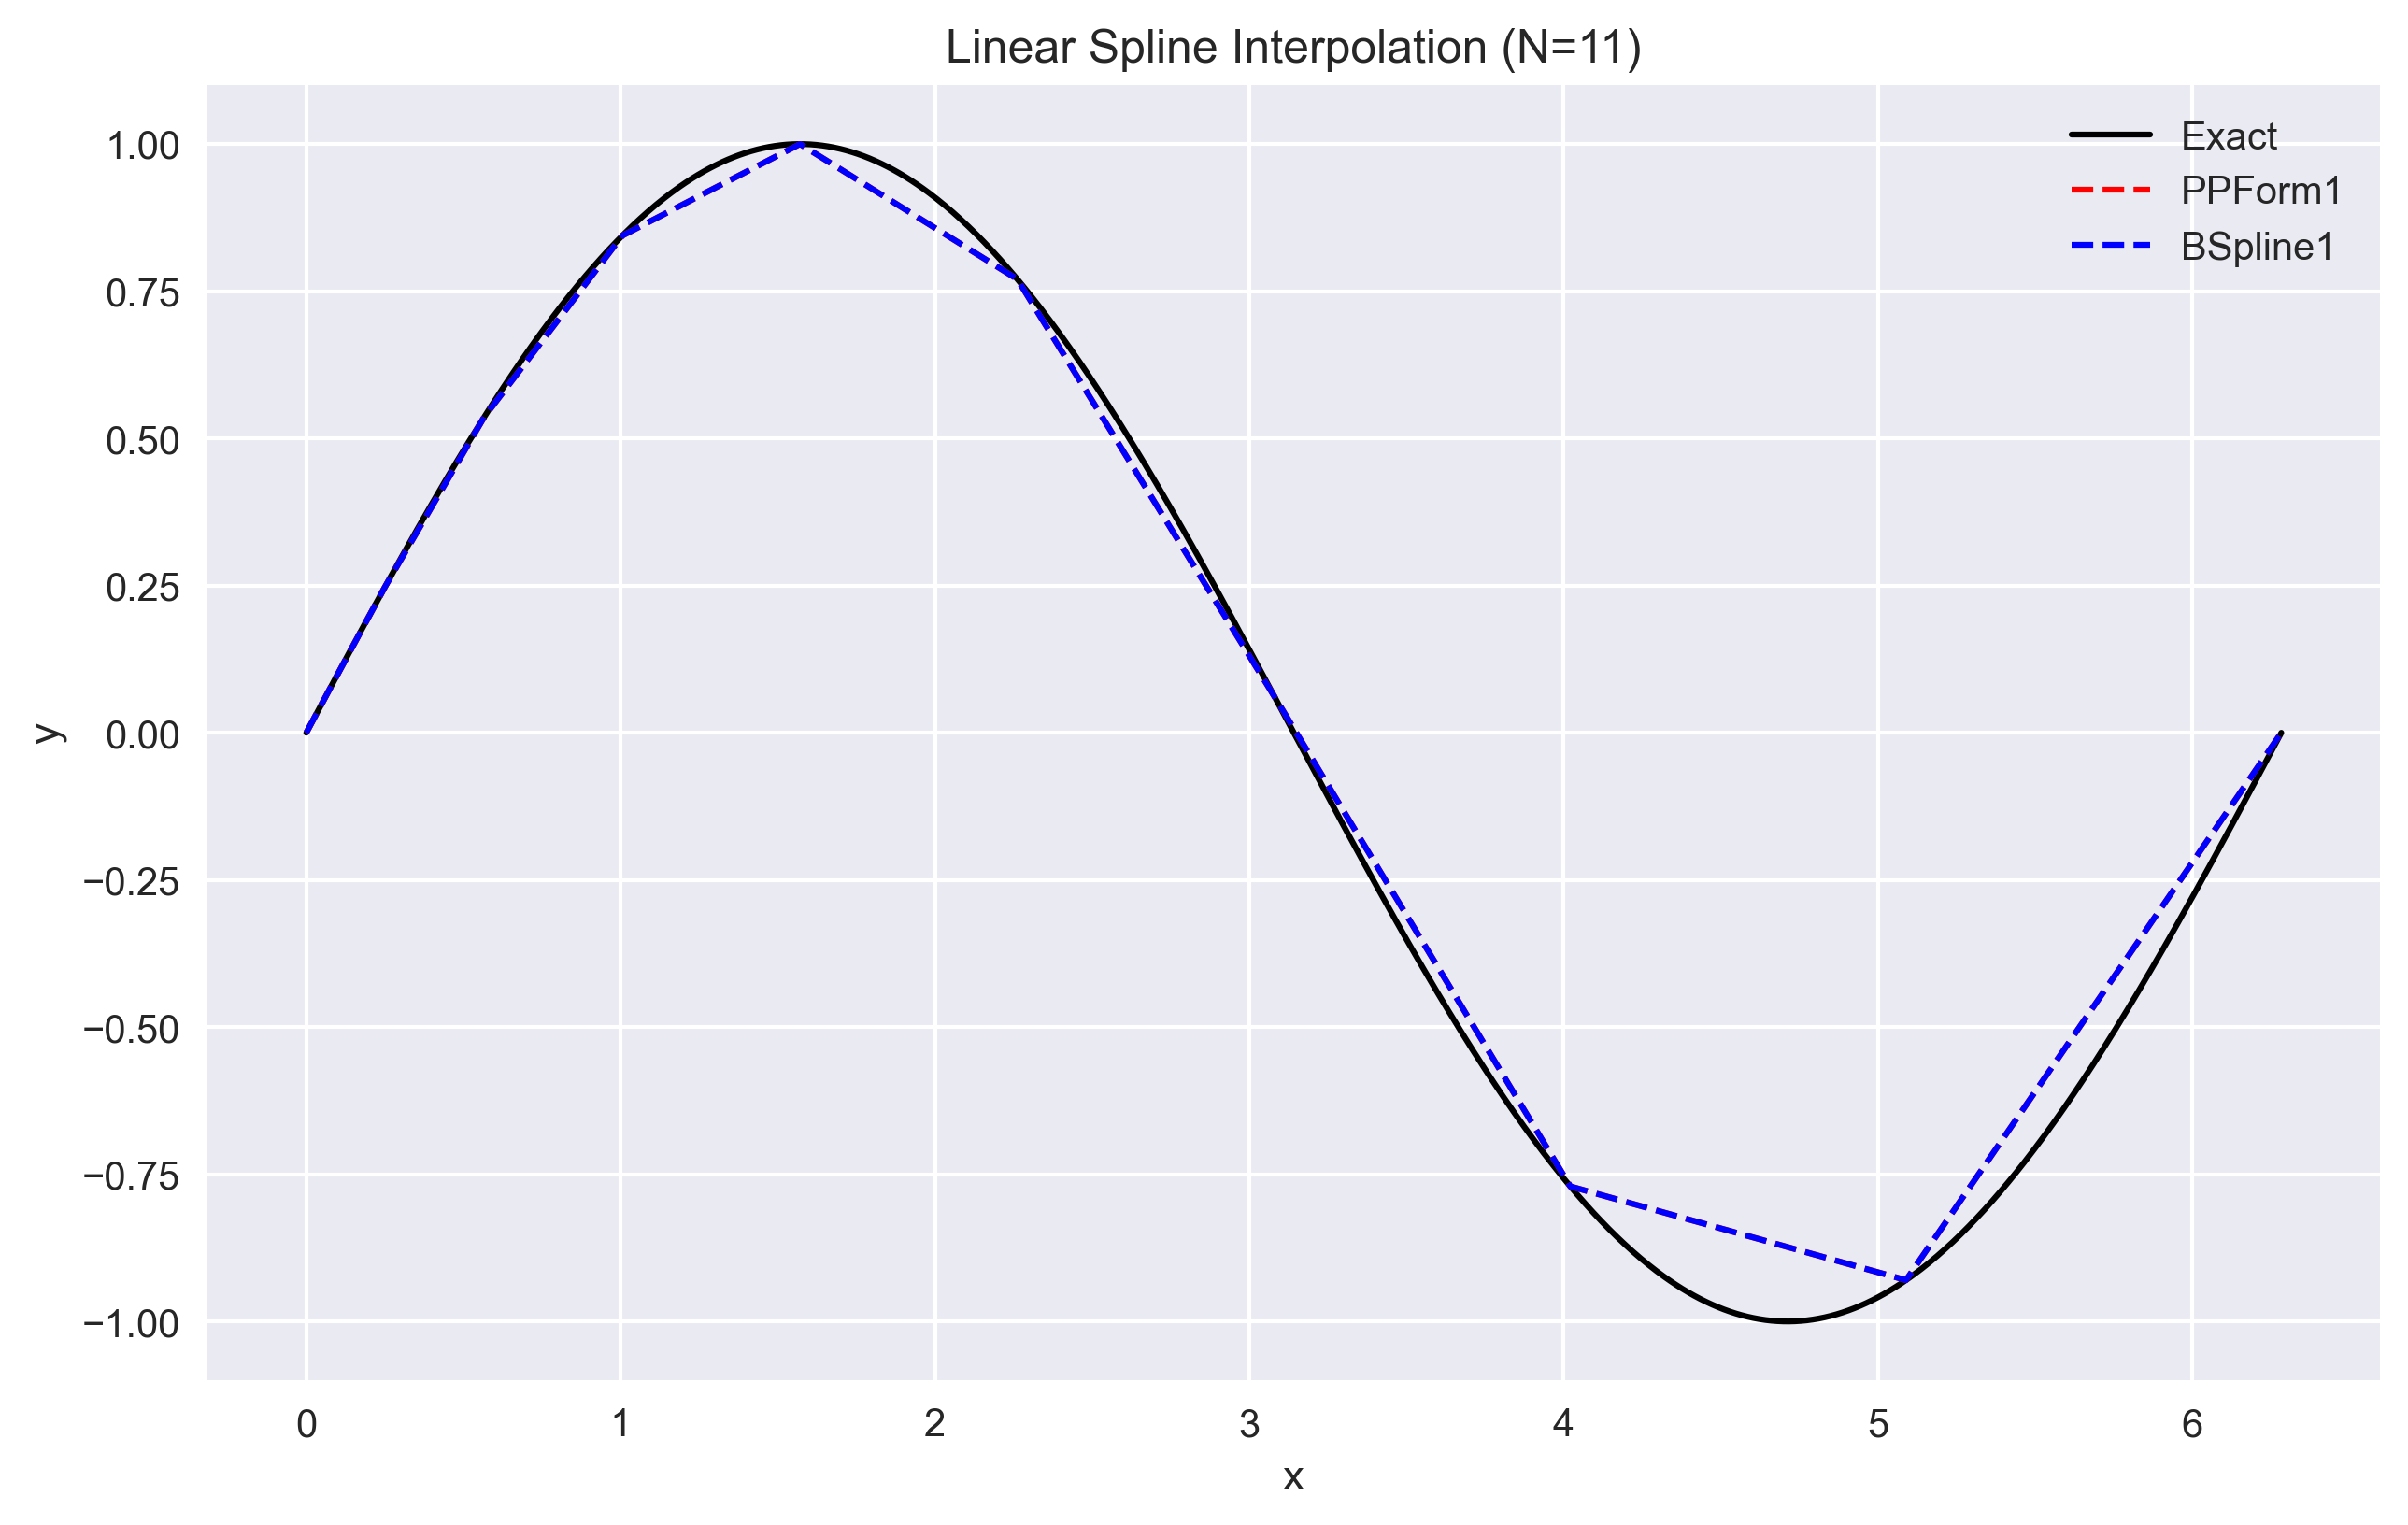
\includegraphics[width=0.45\textwidth]{../figure/test/linear_N11.png} &
    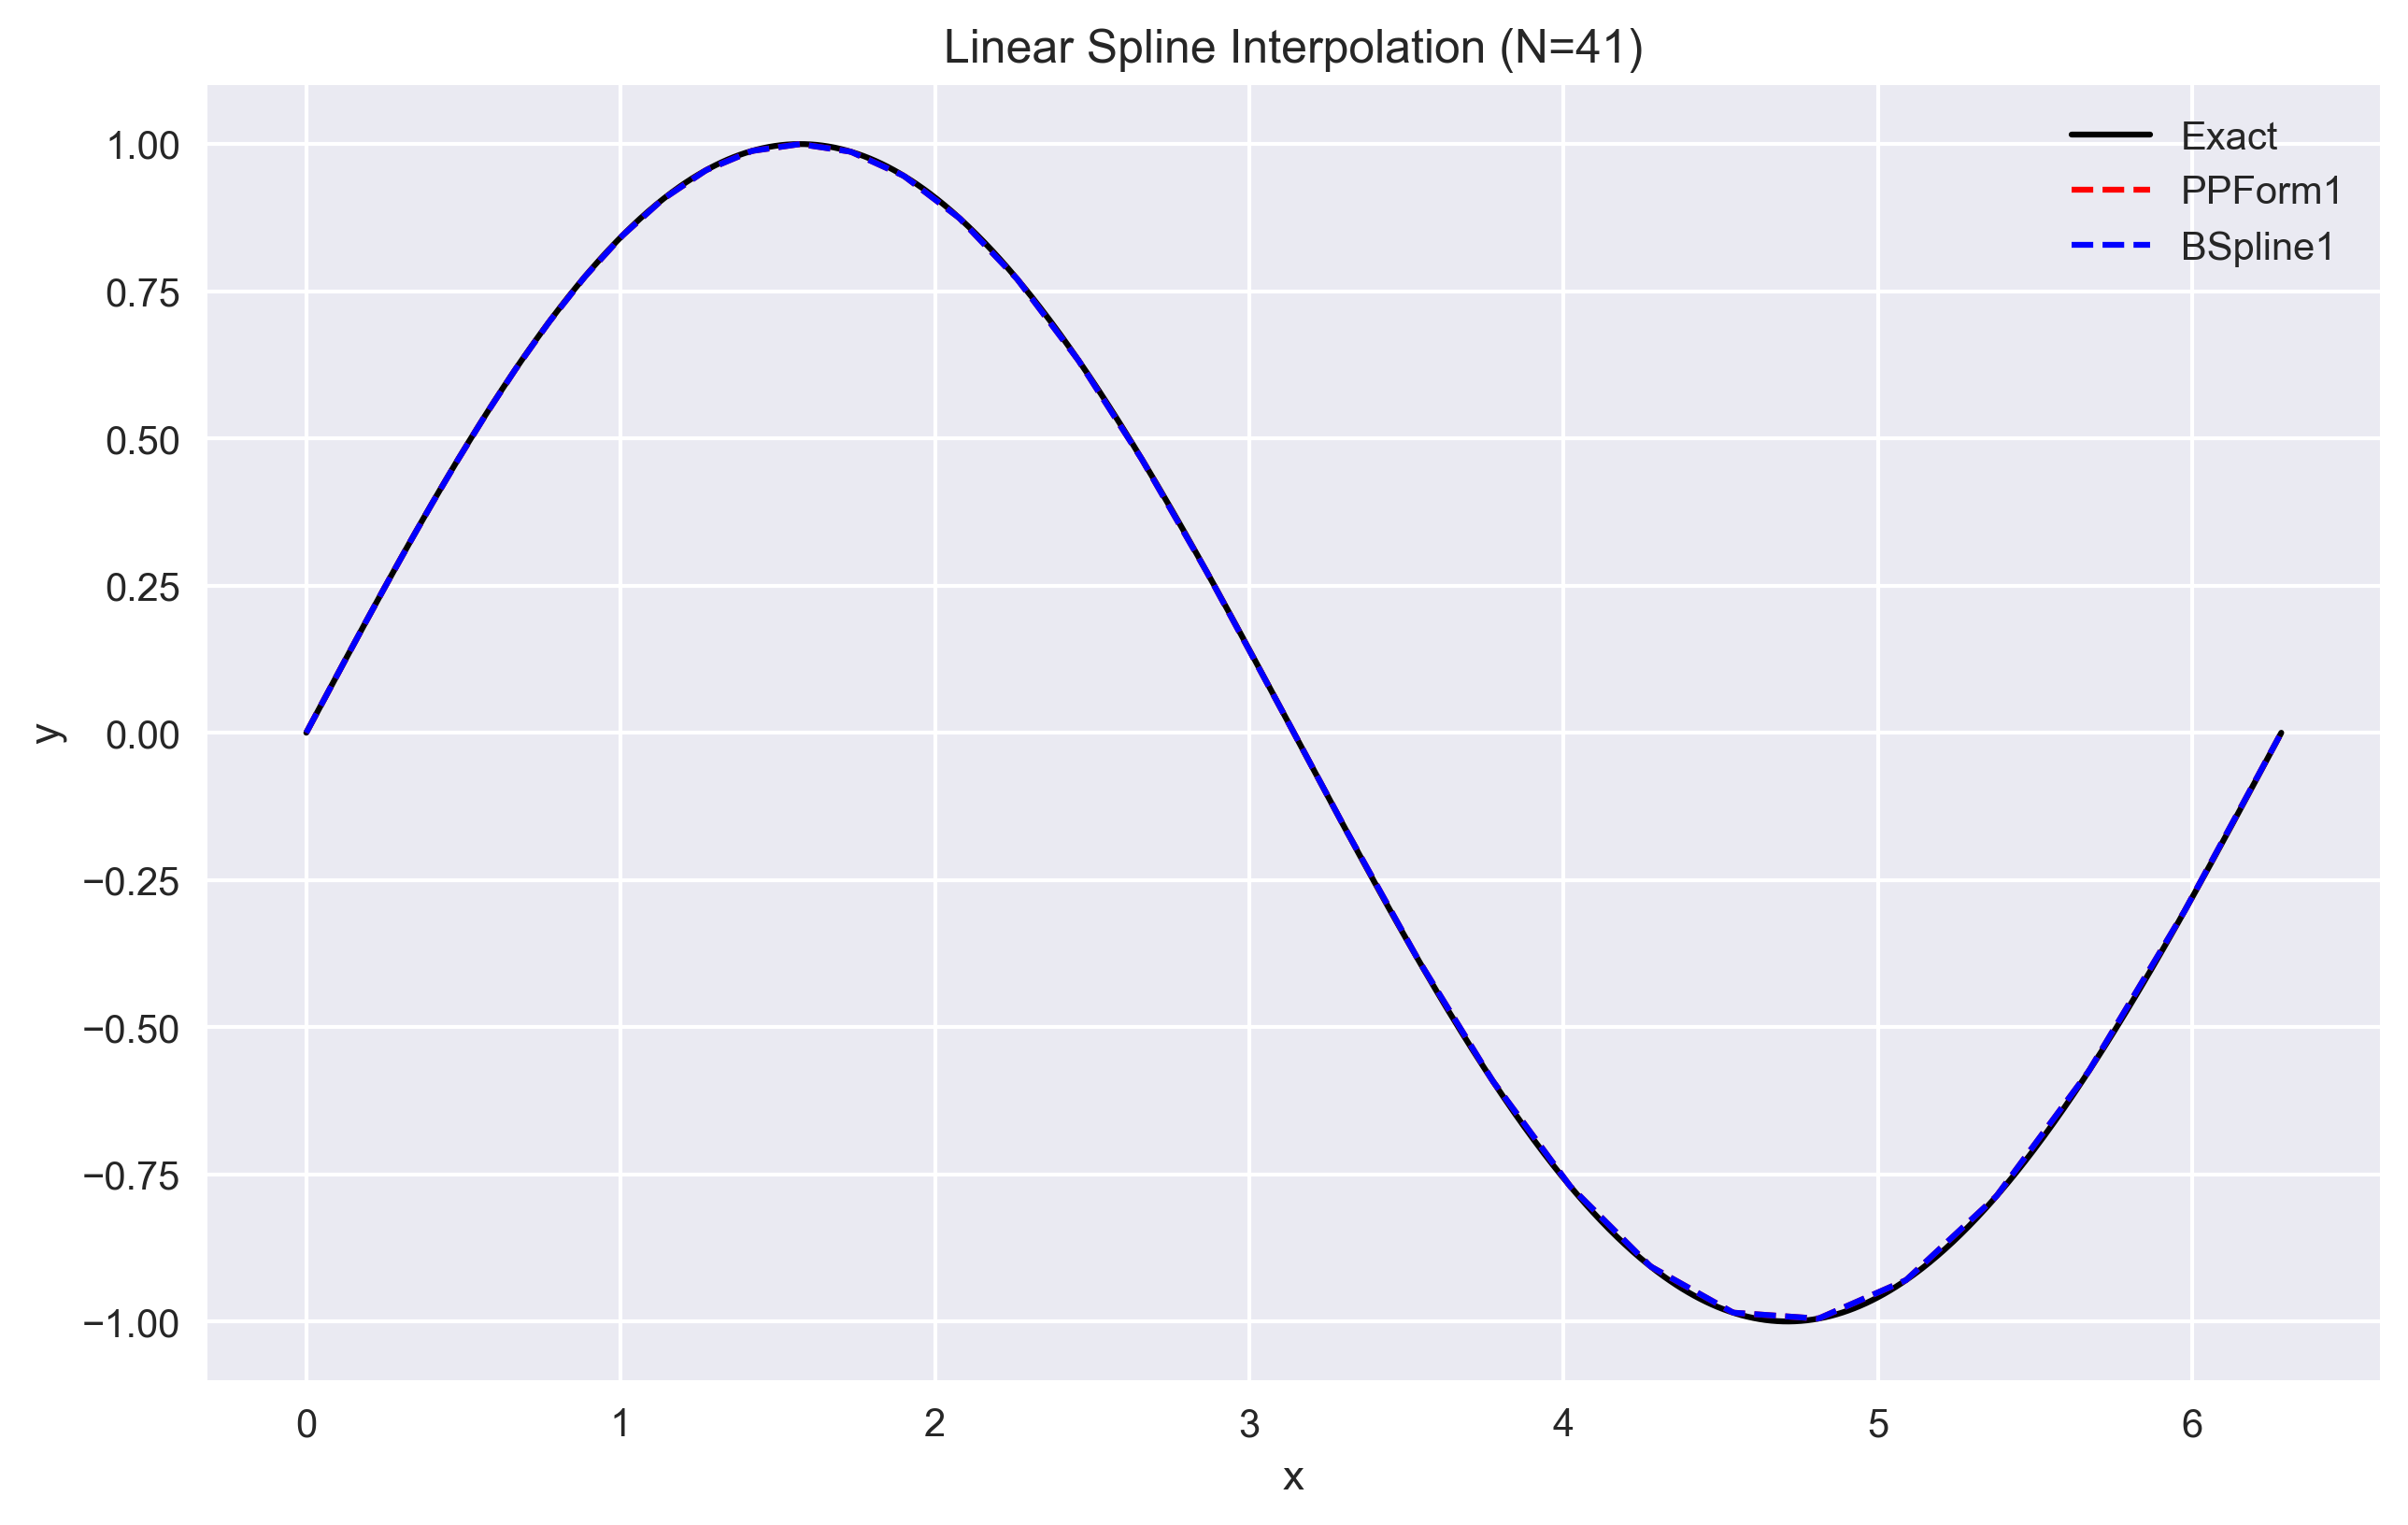
\includegraphics[width=0.45\textwidth]{../figure/test/linear_N41.png}   \\
    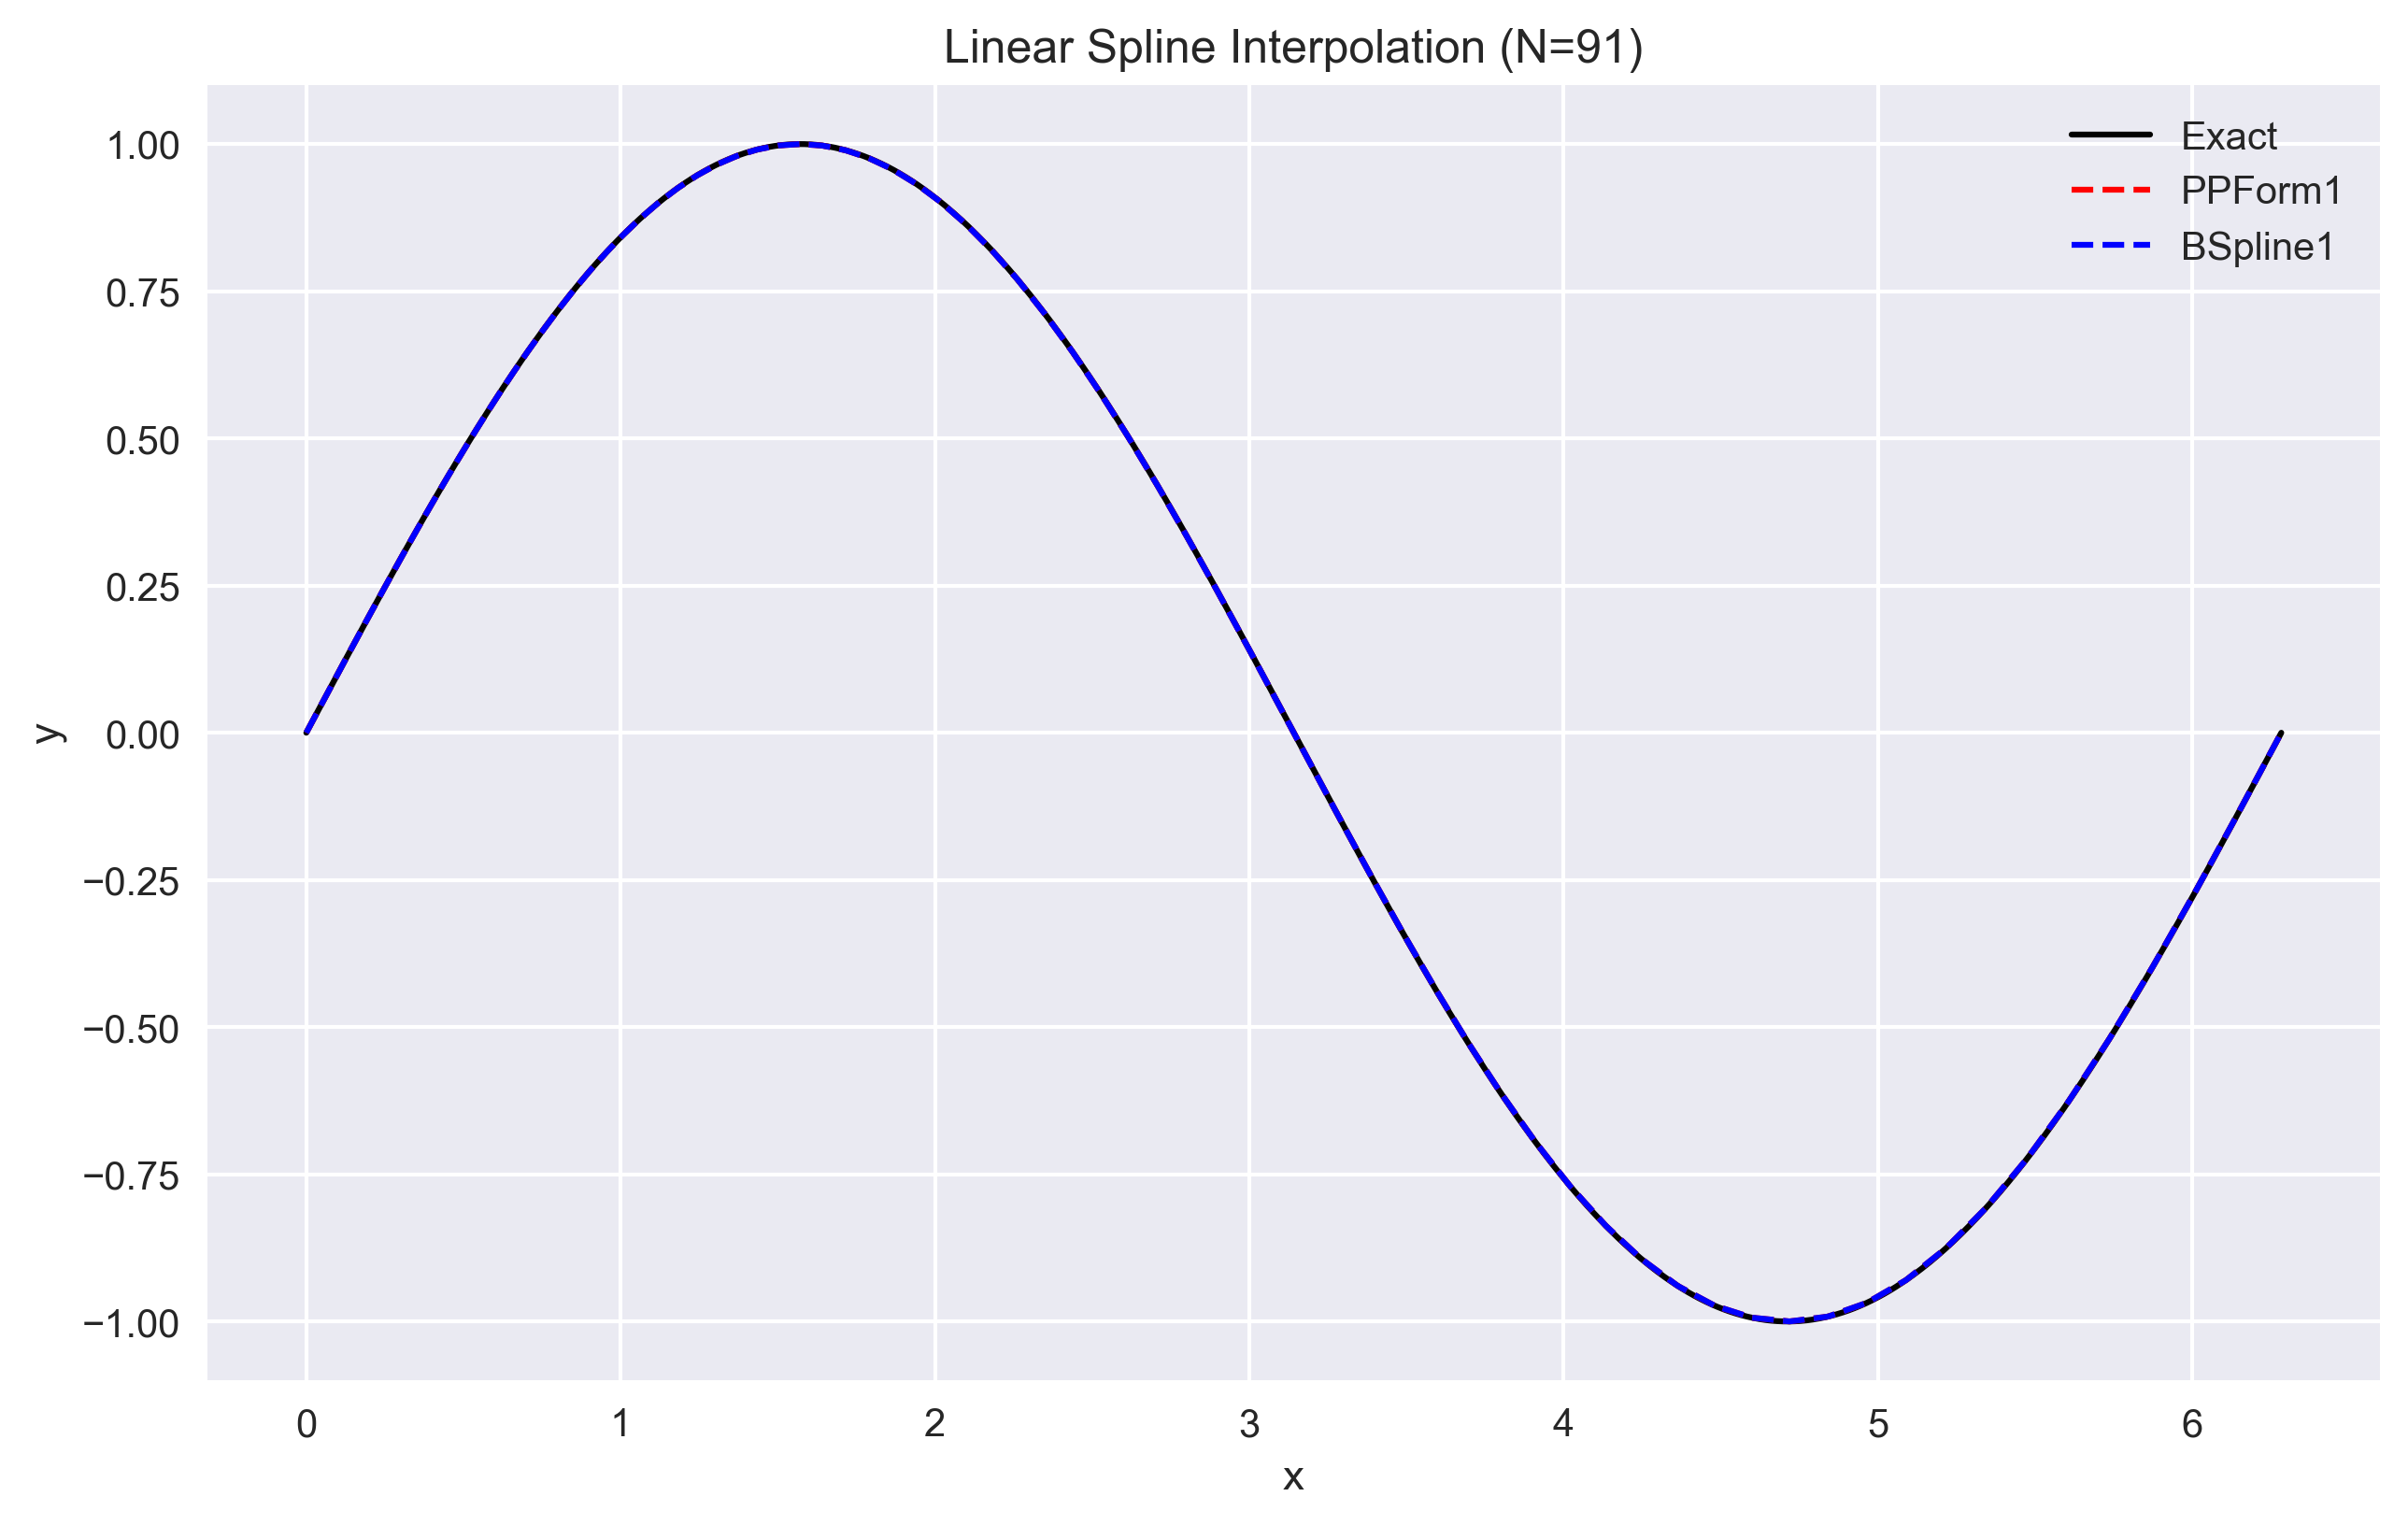
\includegraphics[width=0.45\textwidth]{../figure/test/linear_N91.png} &
  \end{tabular}
  \renewcommand{\figurename}{Fig.}
  \caption{Linear PPForm and BSpline interpolation for different \(N\) values}
  \label{fig:test_linear}
\end{figure}

As shown in Fig.\ref{fig:test_quadratic}, below are the interpolation results of third-order PPForm and BSpline interpolation for different values of \(N\).

\begin{figure}[H]
  \centering
  \begin{tabular}{cc}
    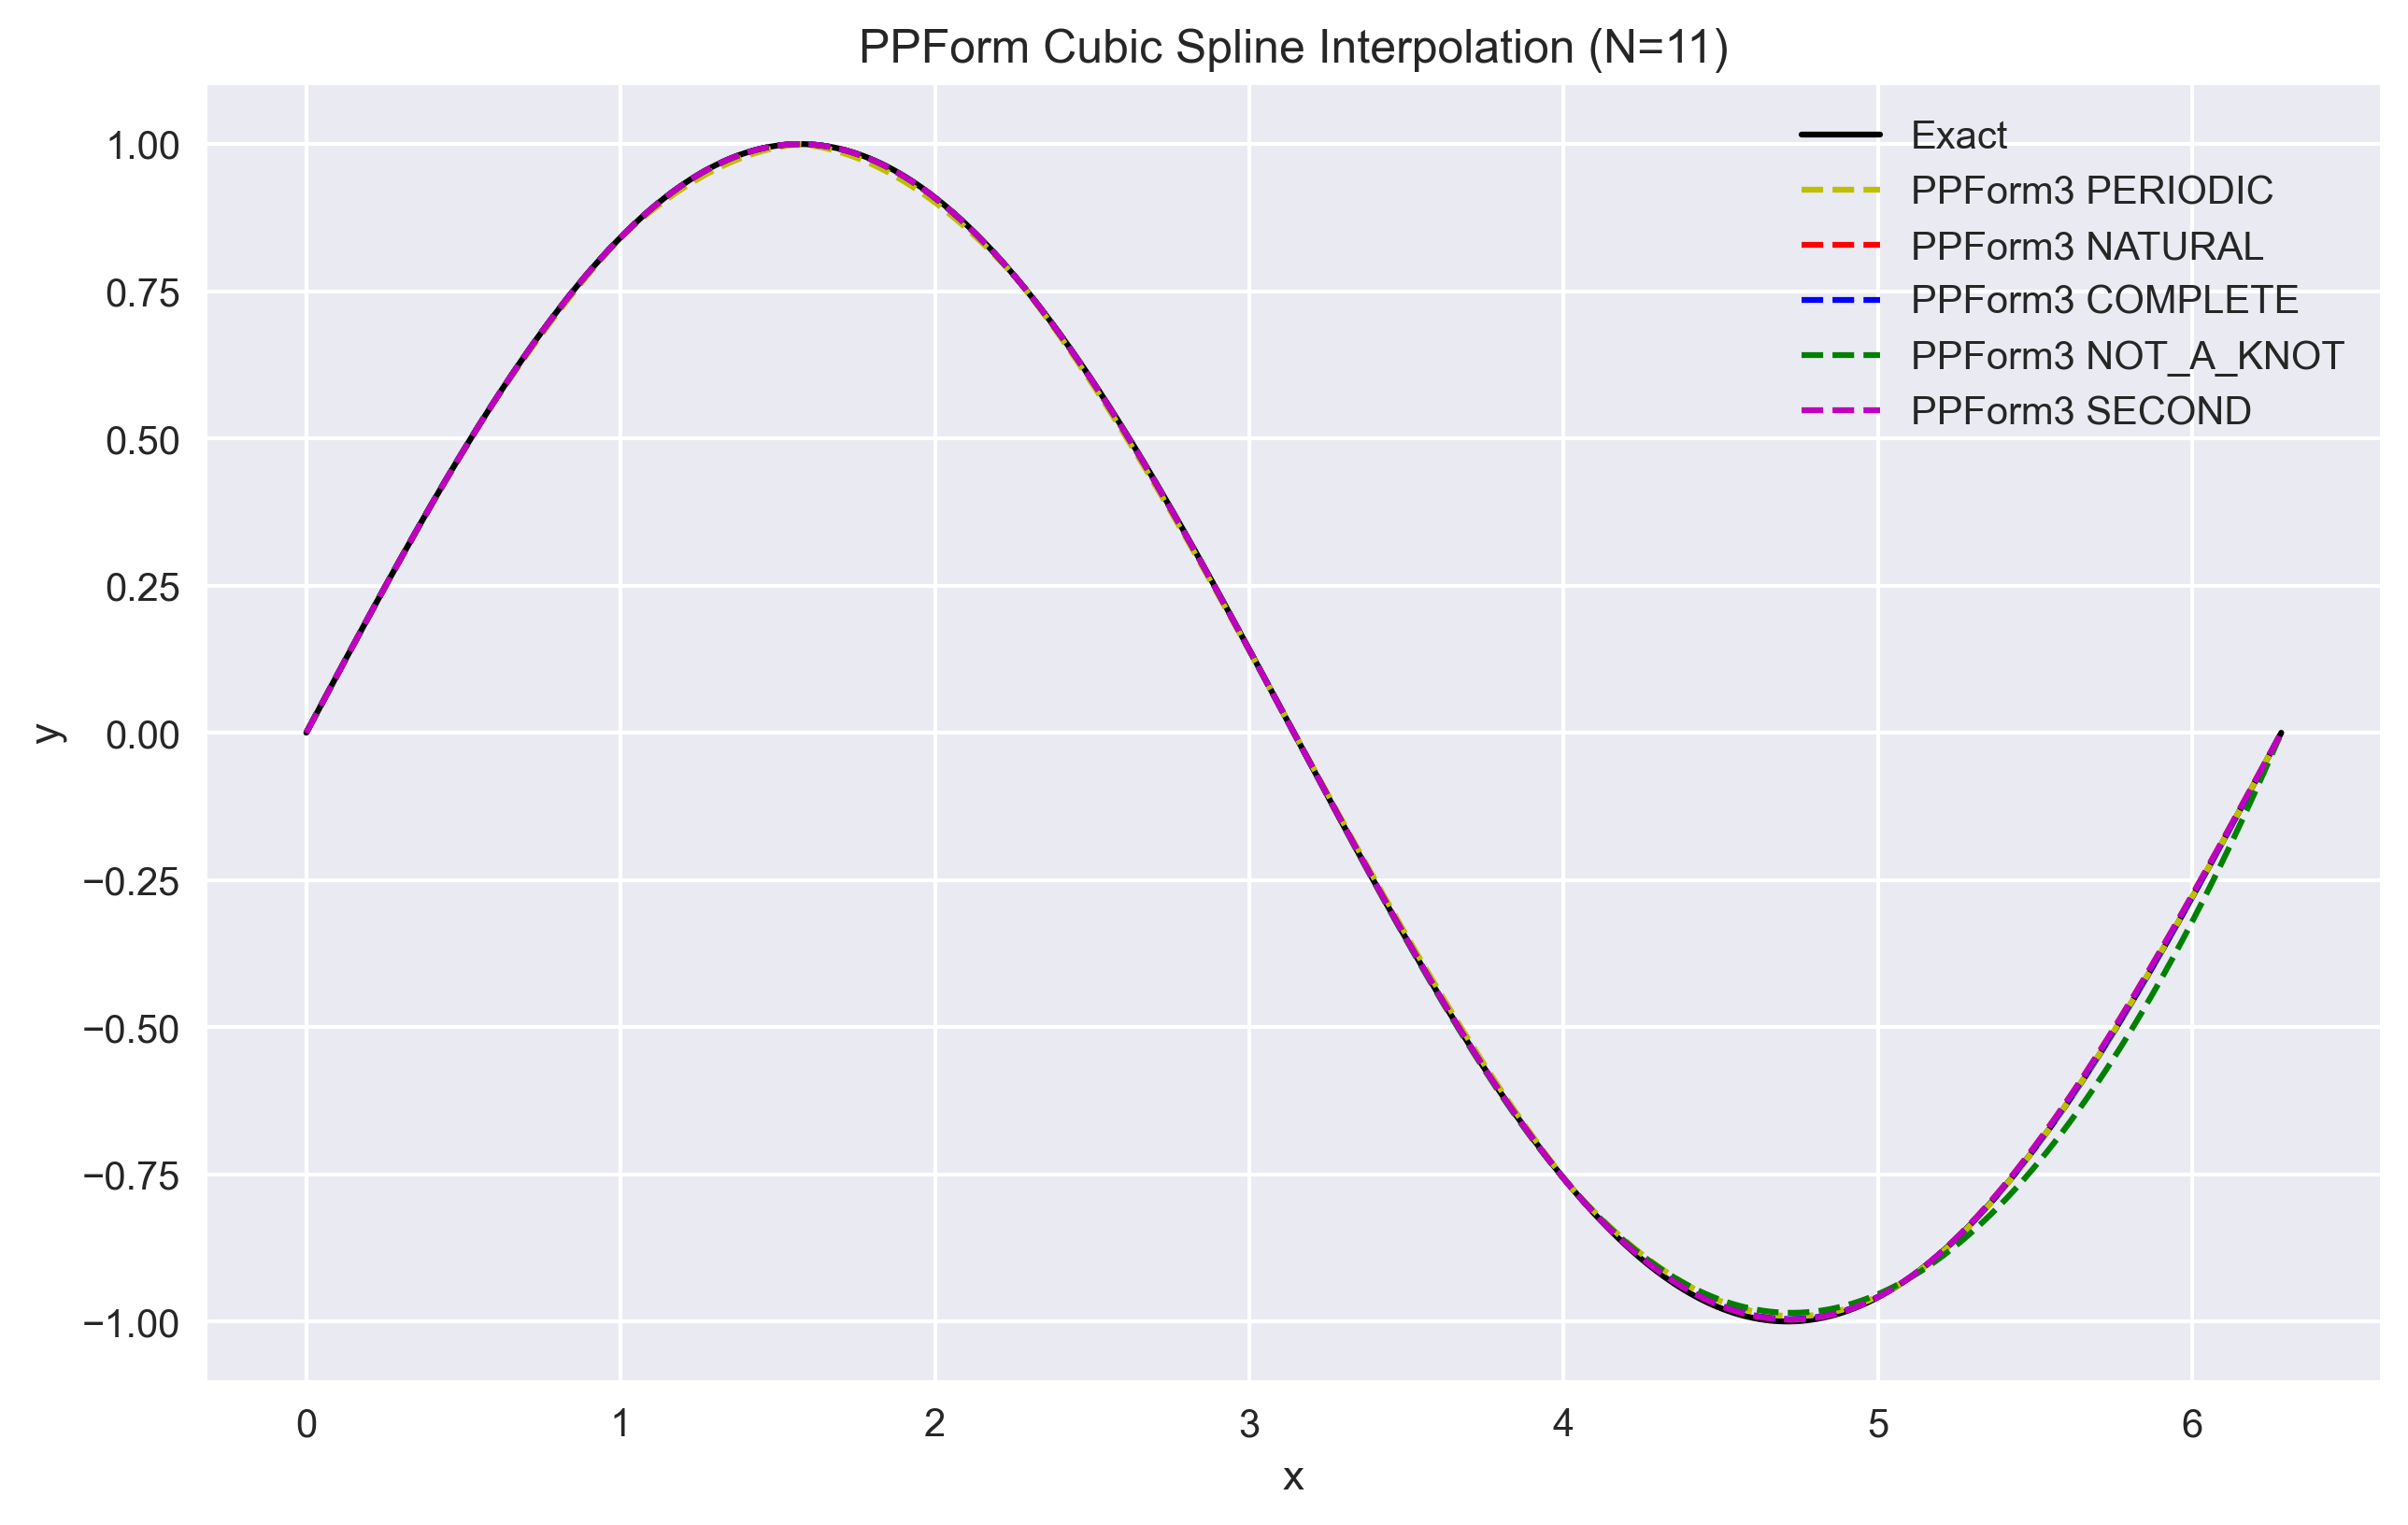
\includegraphics[width=0.45\textwidth]{../figure/test/PPForm3_N11.png} &
    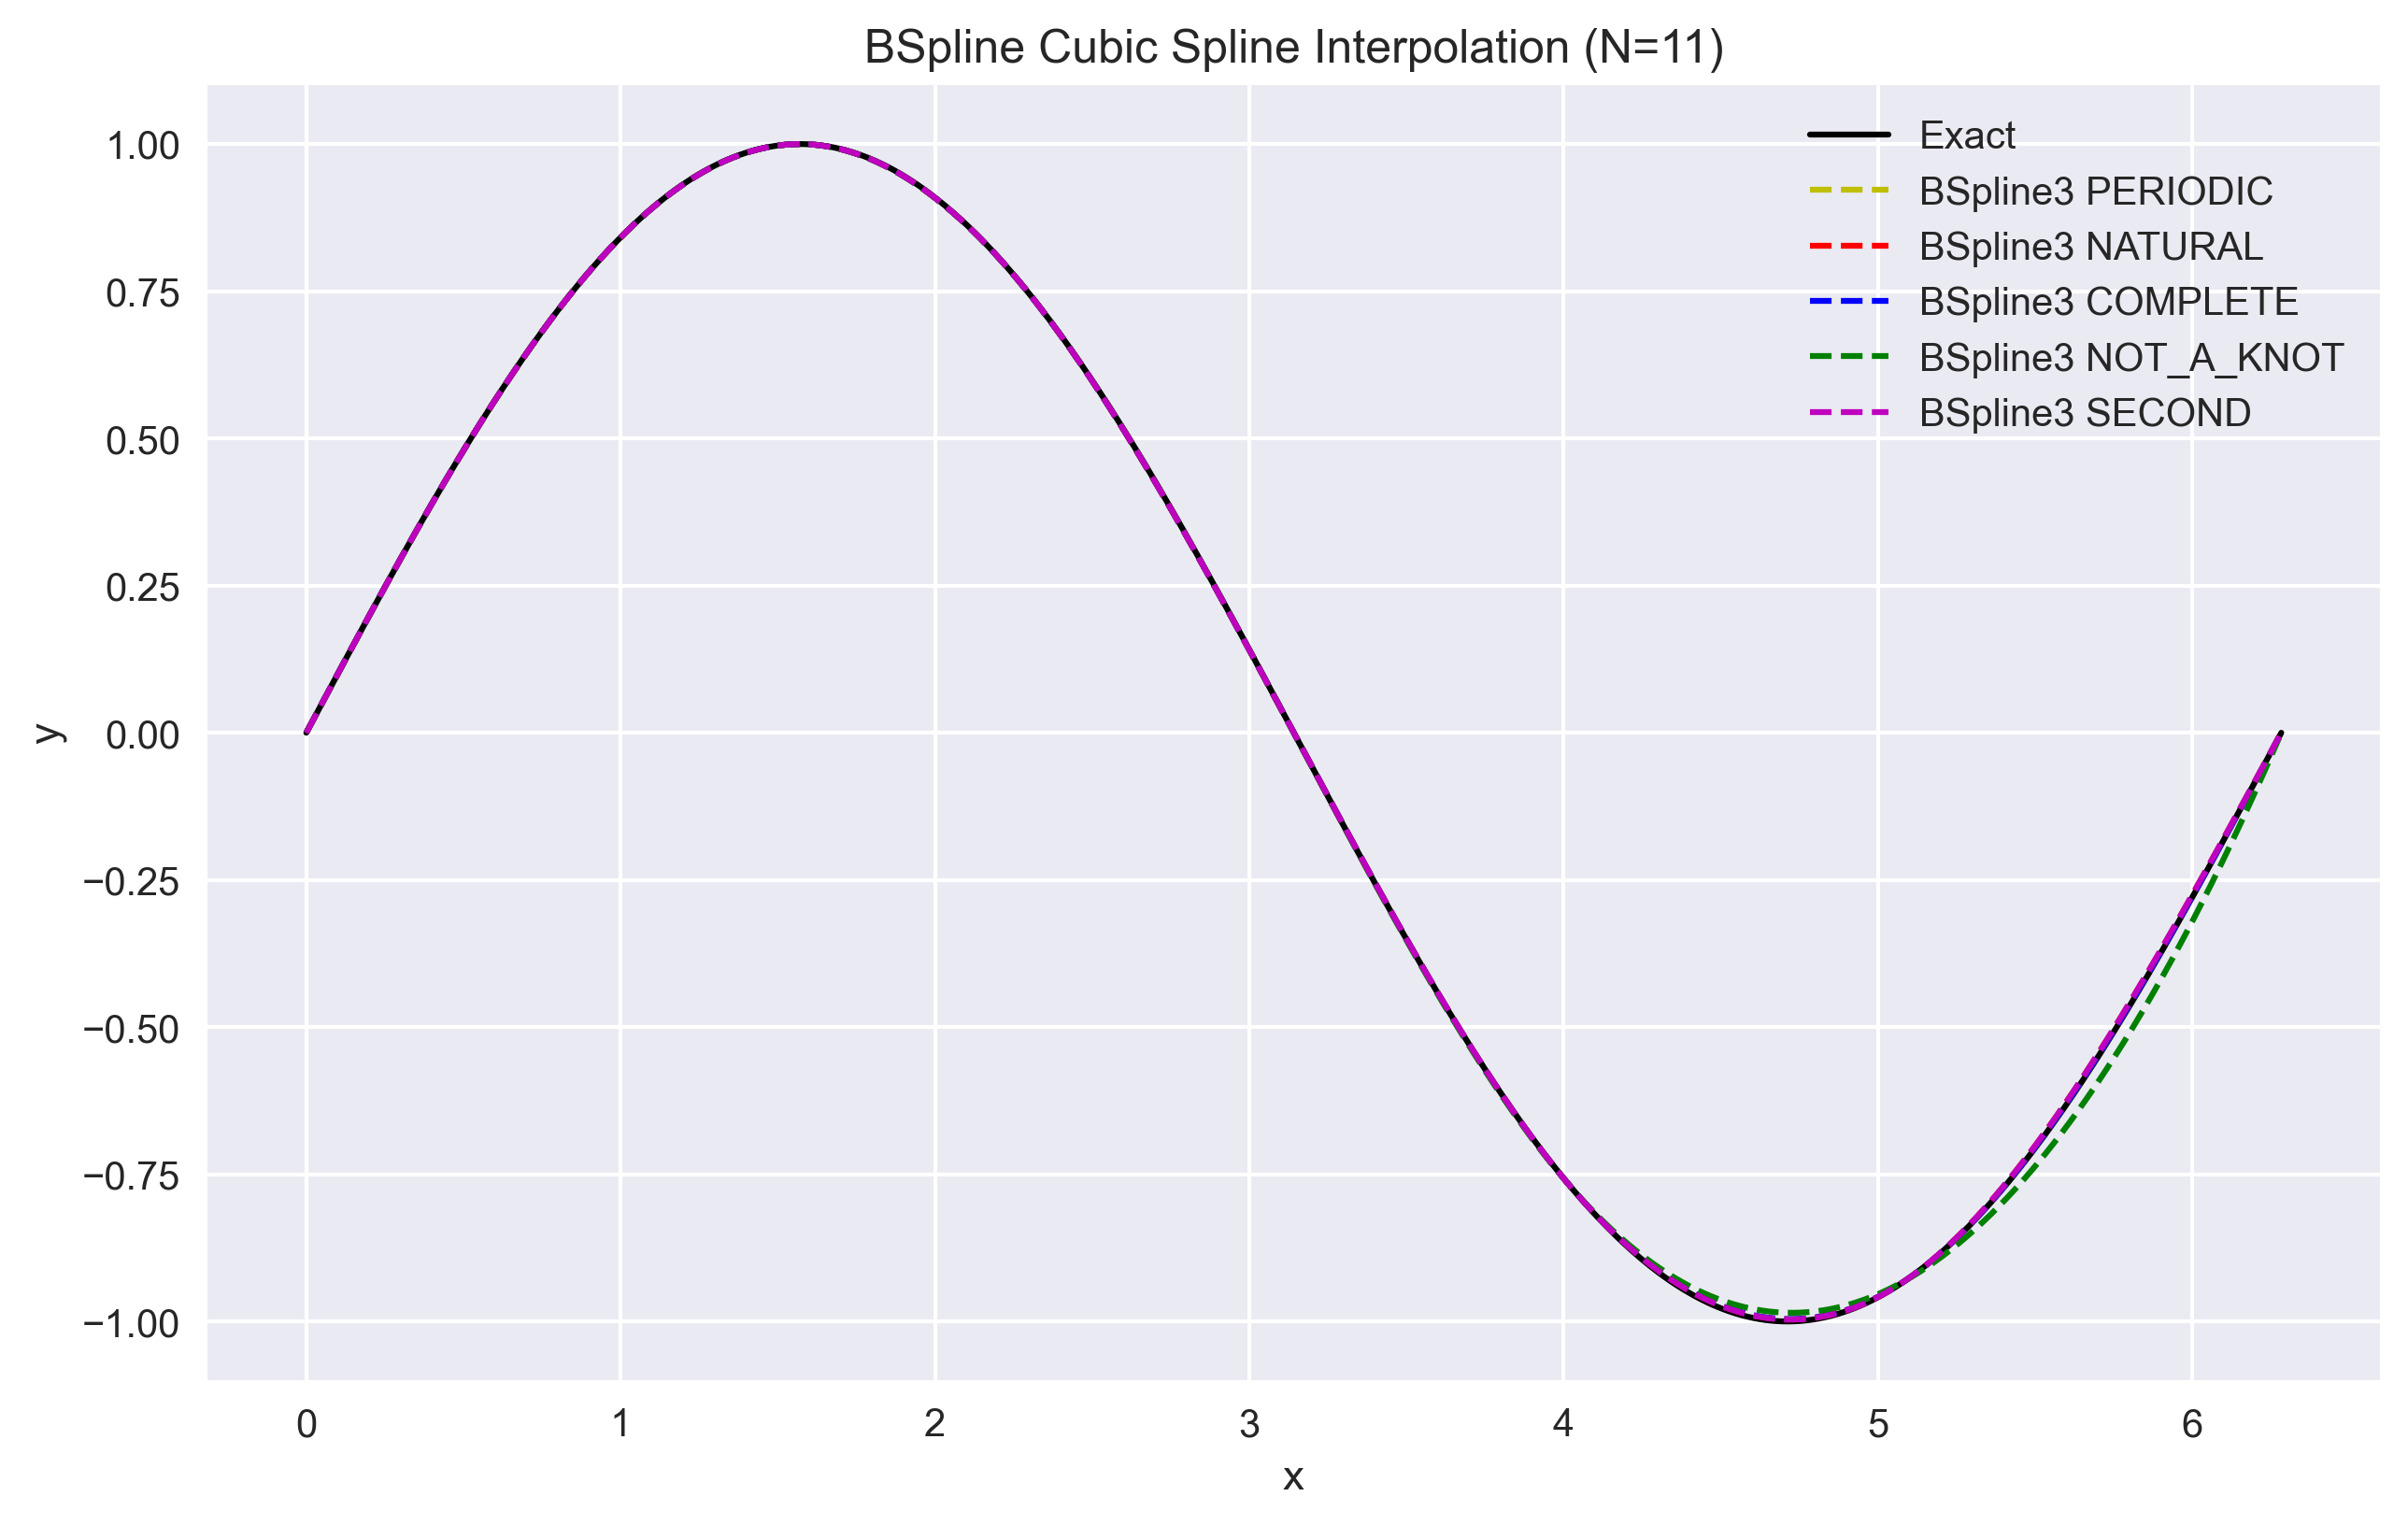
\includegraphics[width=0.45\textwidth]{../figure/test/BSpline3_N11.png}  \\
    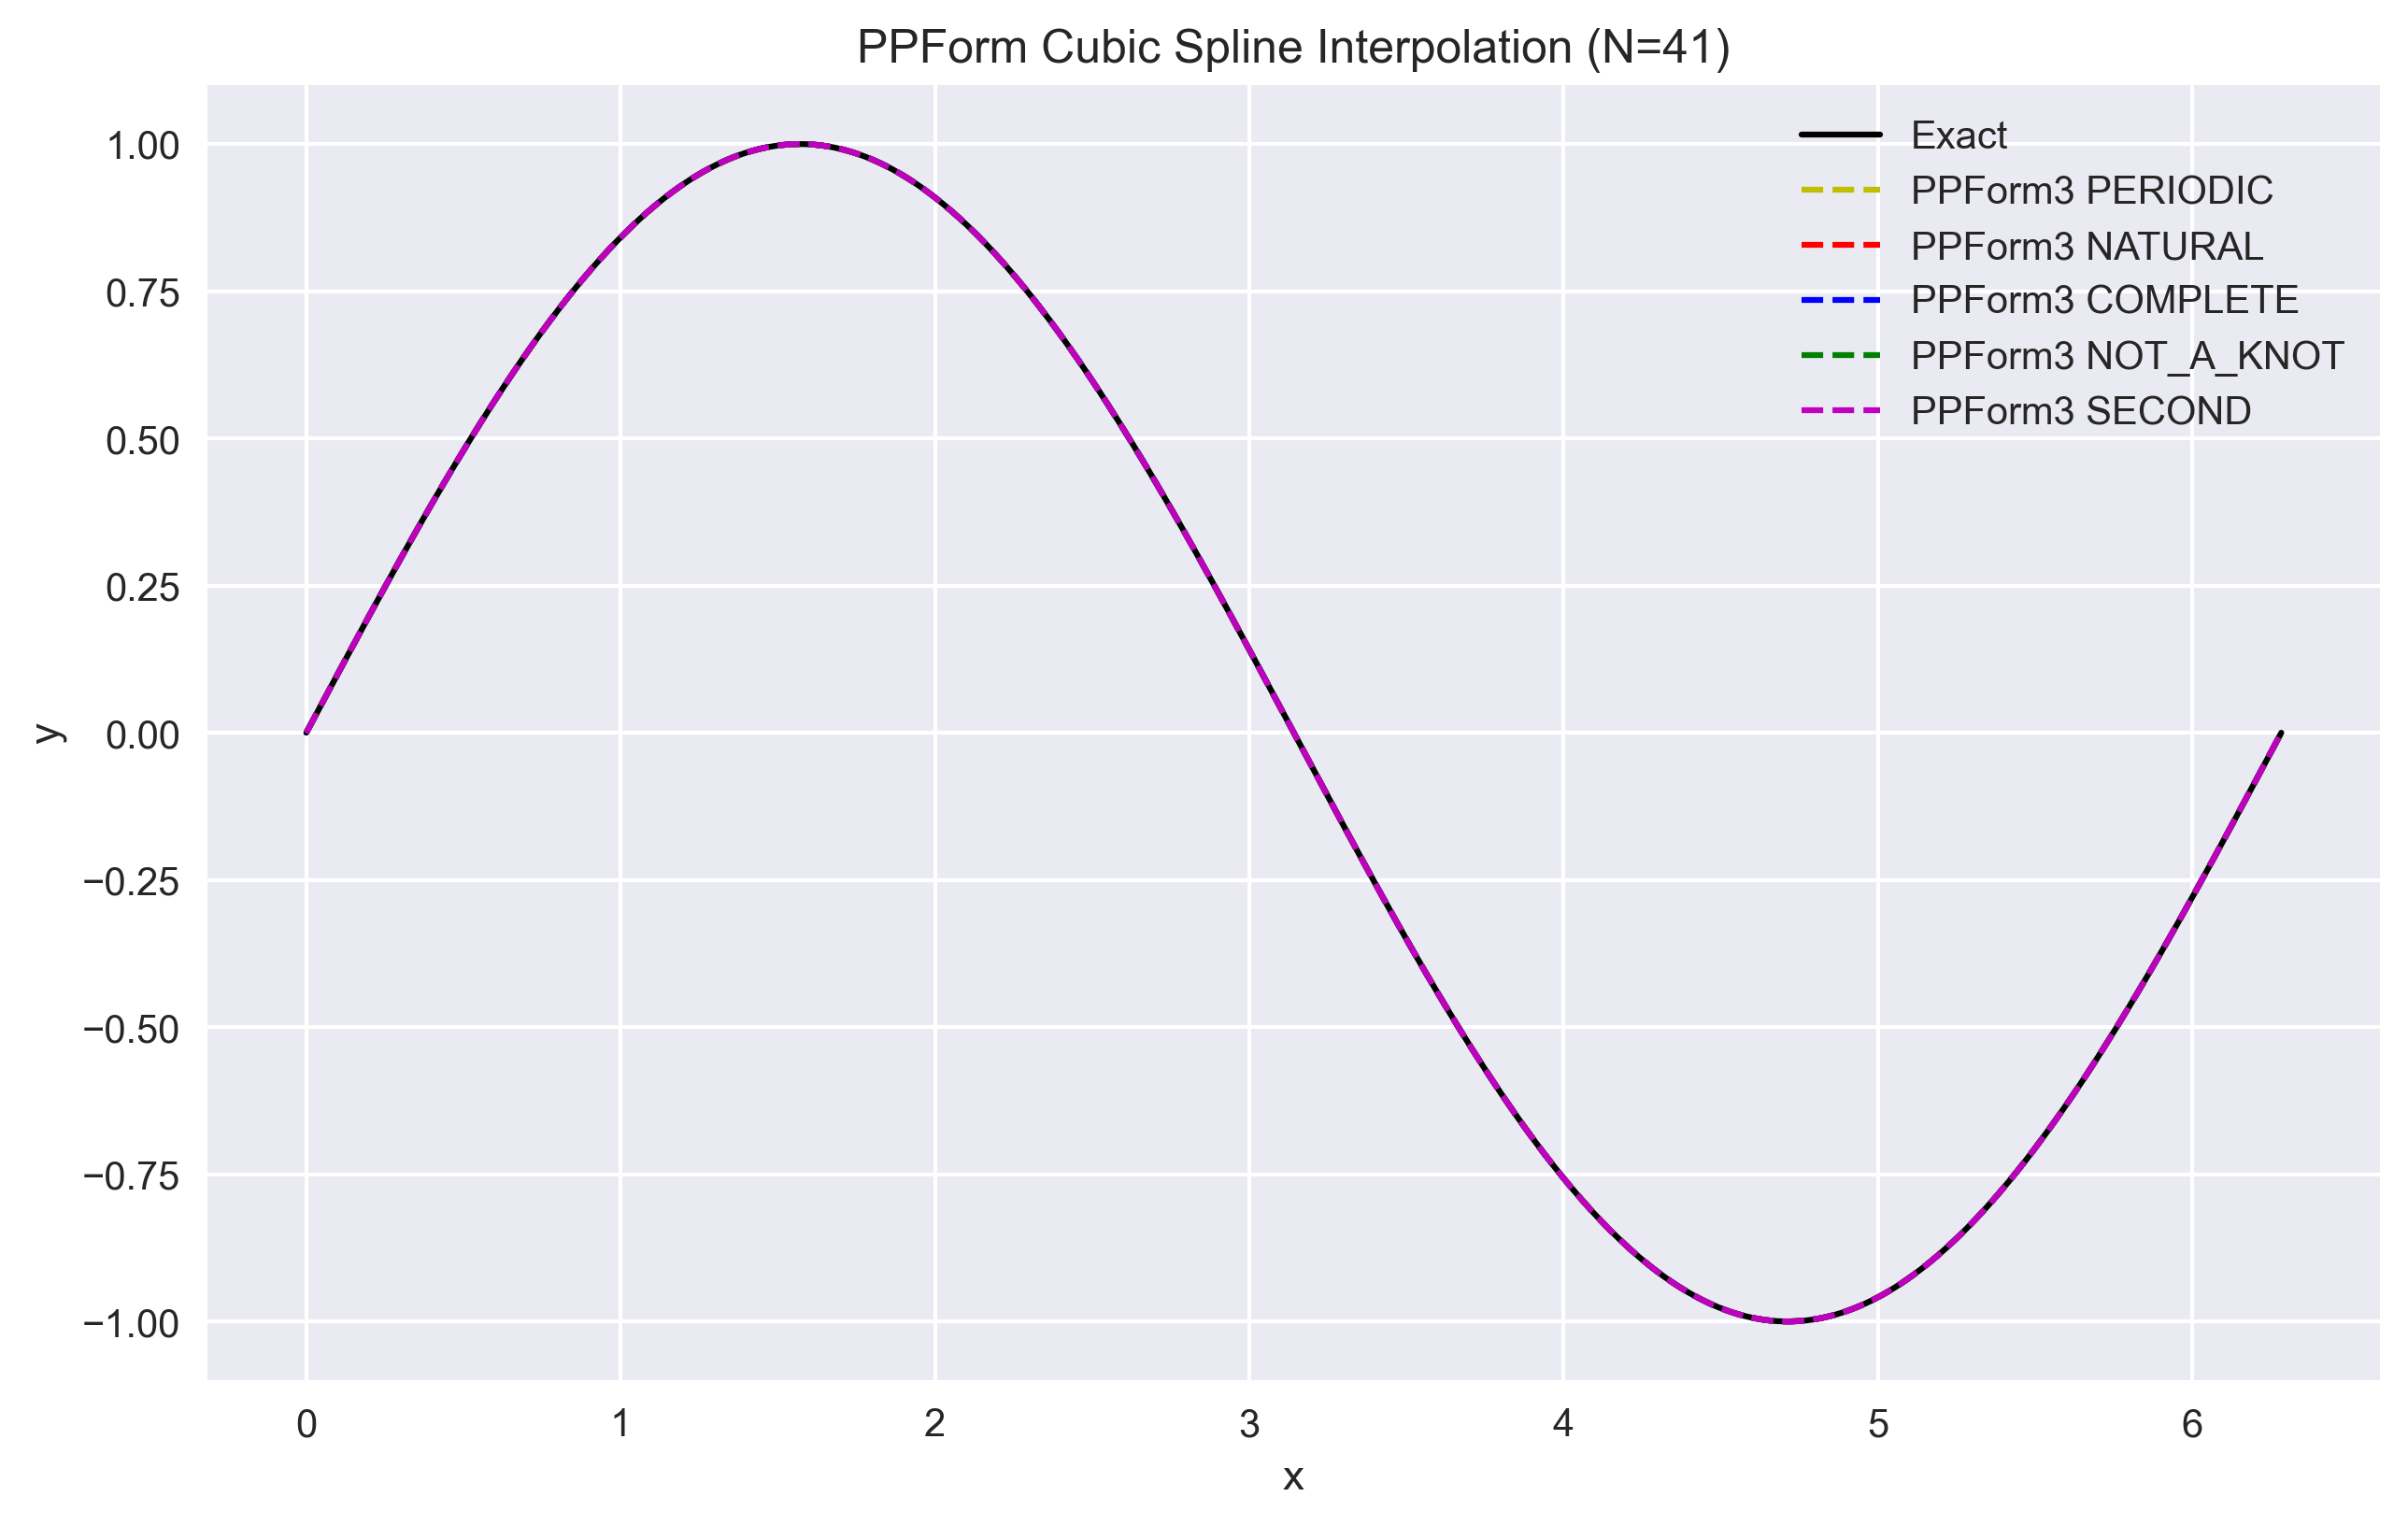
\includegraphics[width=0.45\textwidth]{../figure/test/PPForm3_N41.png} &
    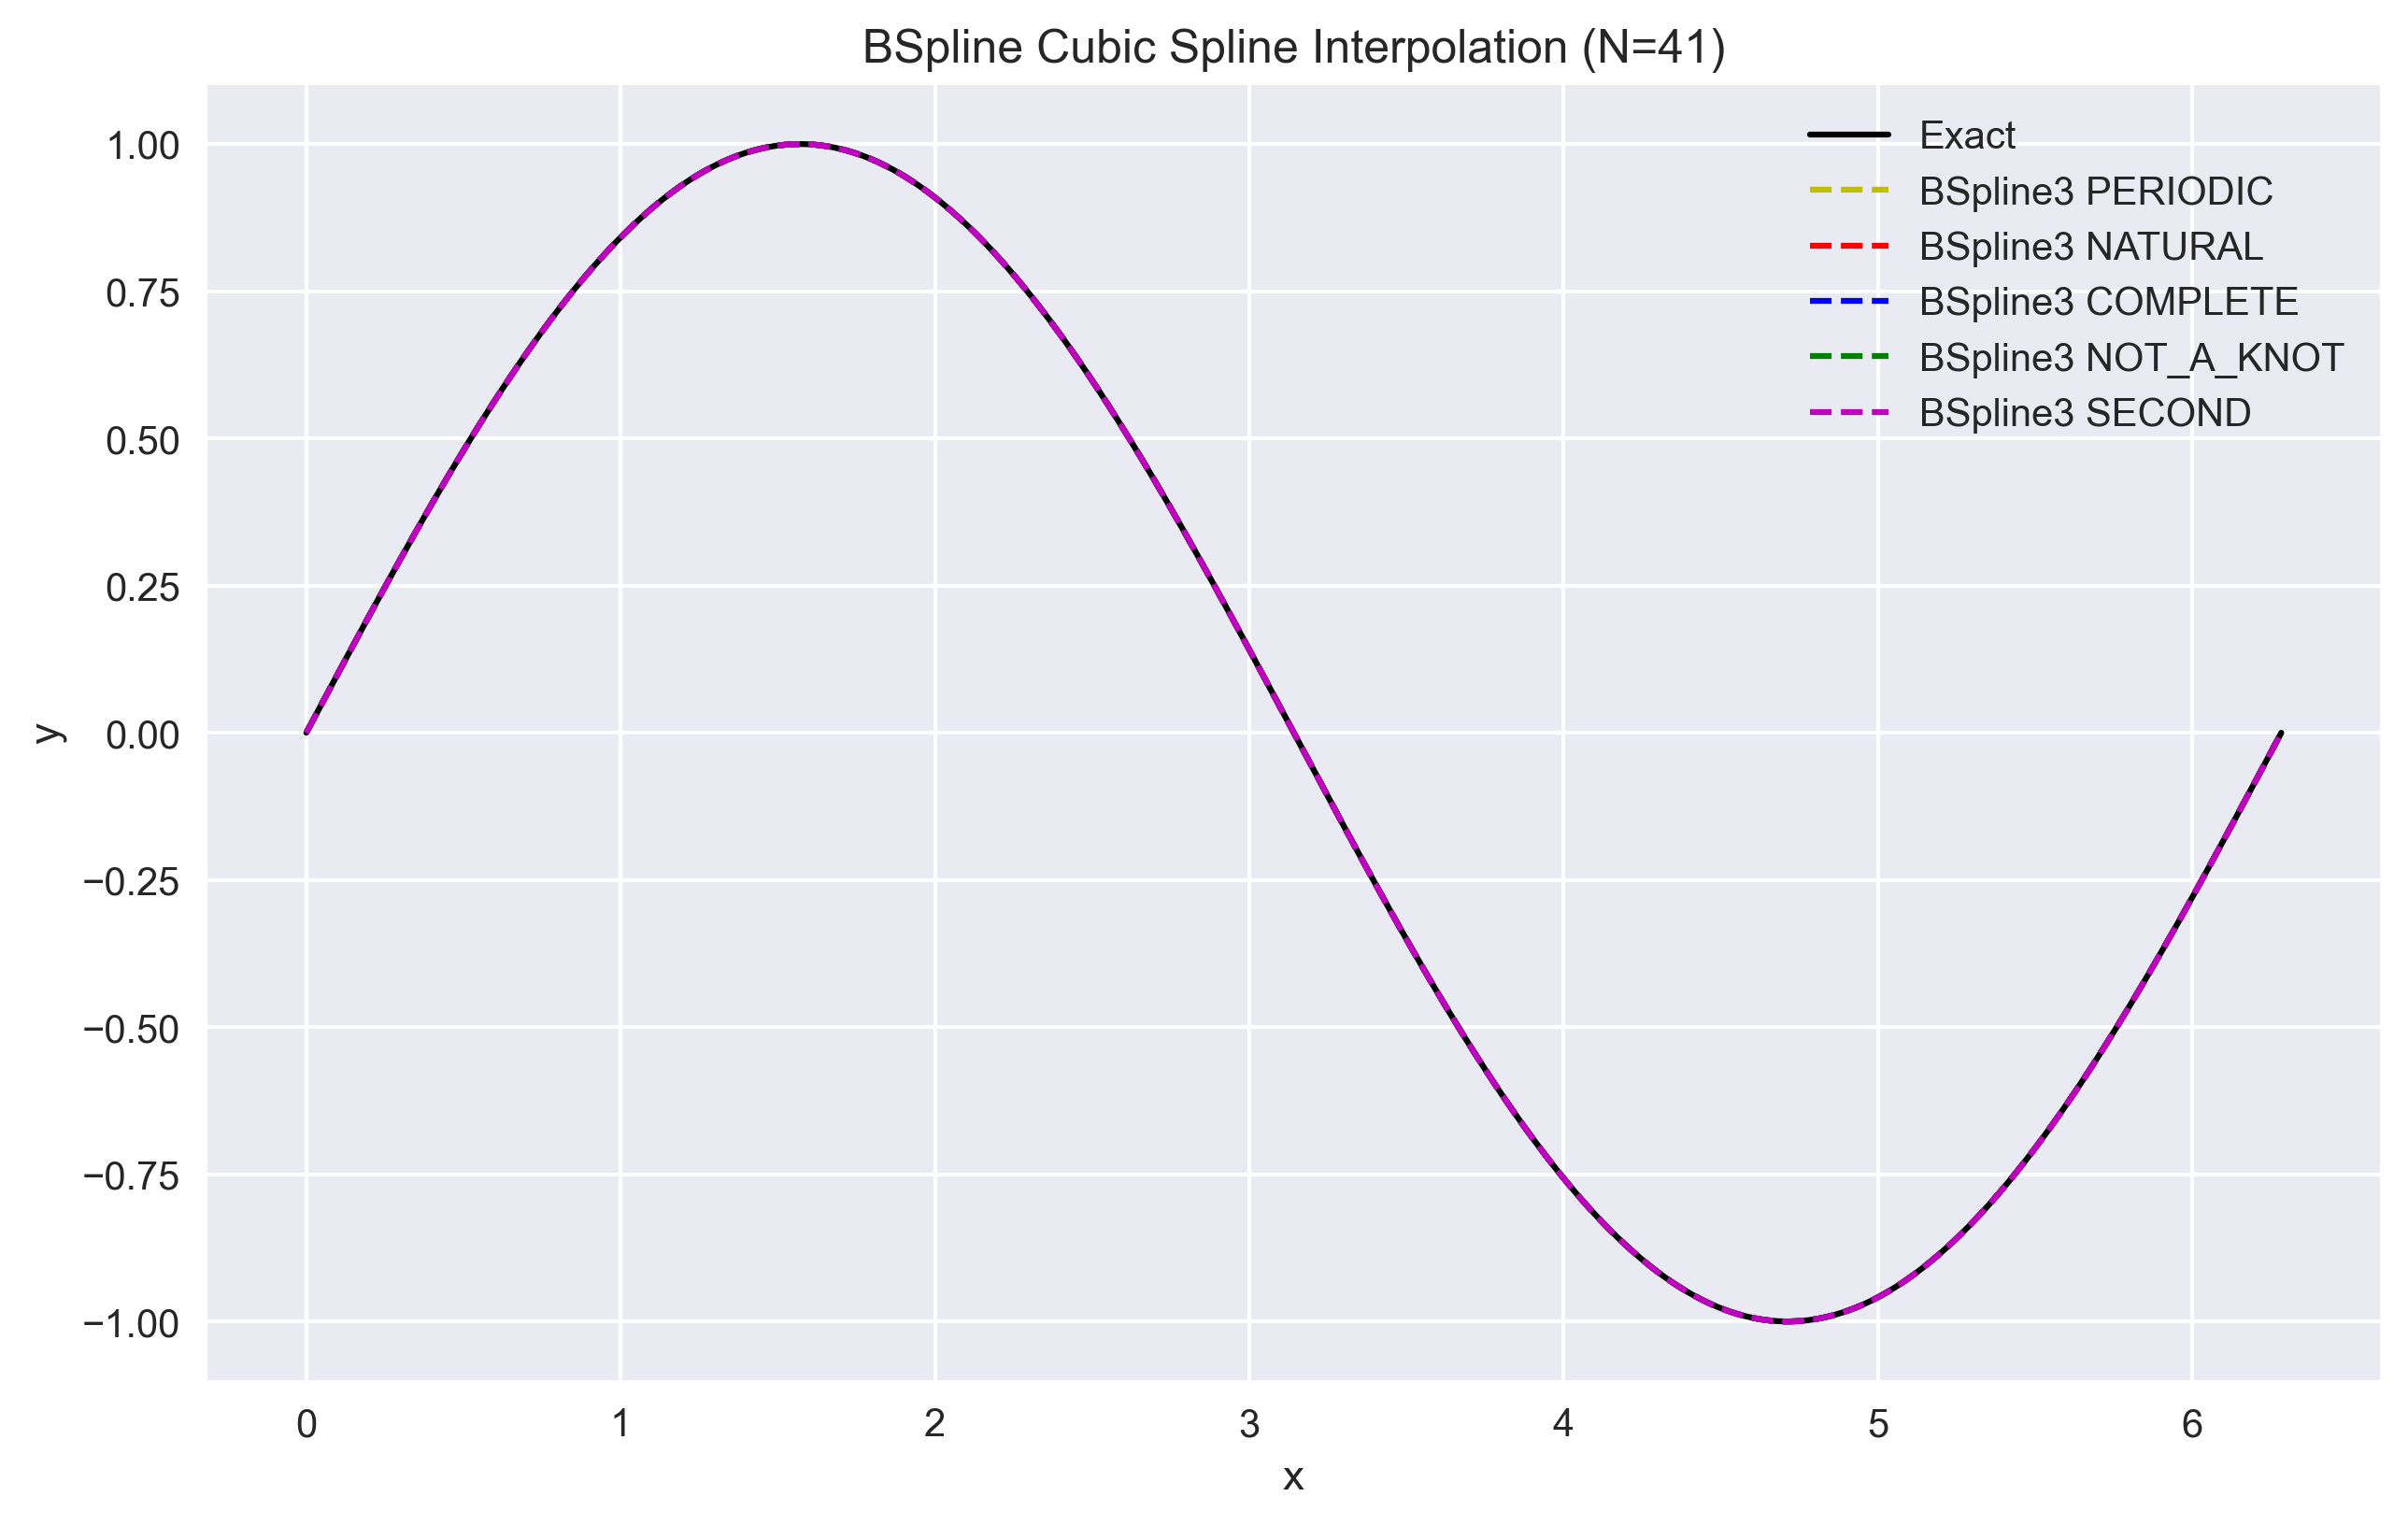
\includegraphics[width=0.45\textwidth]{../figure/test/BSpline3_N41.png}  \\
    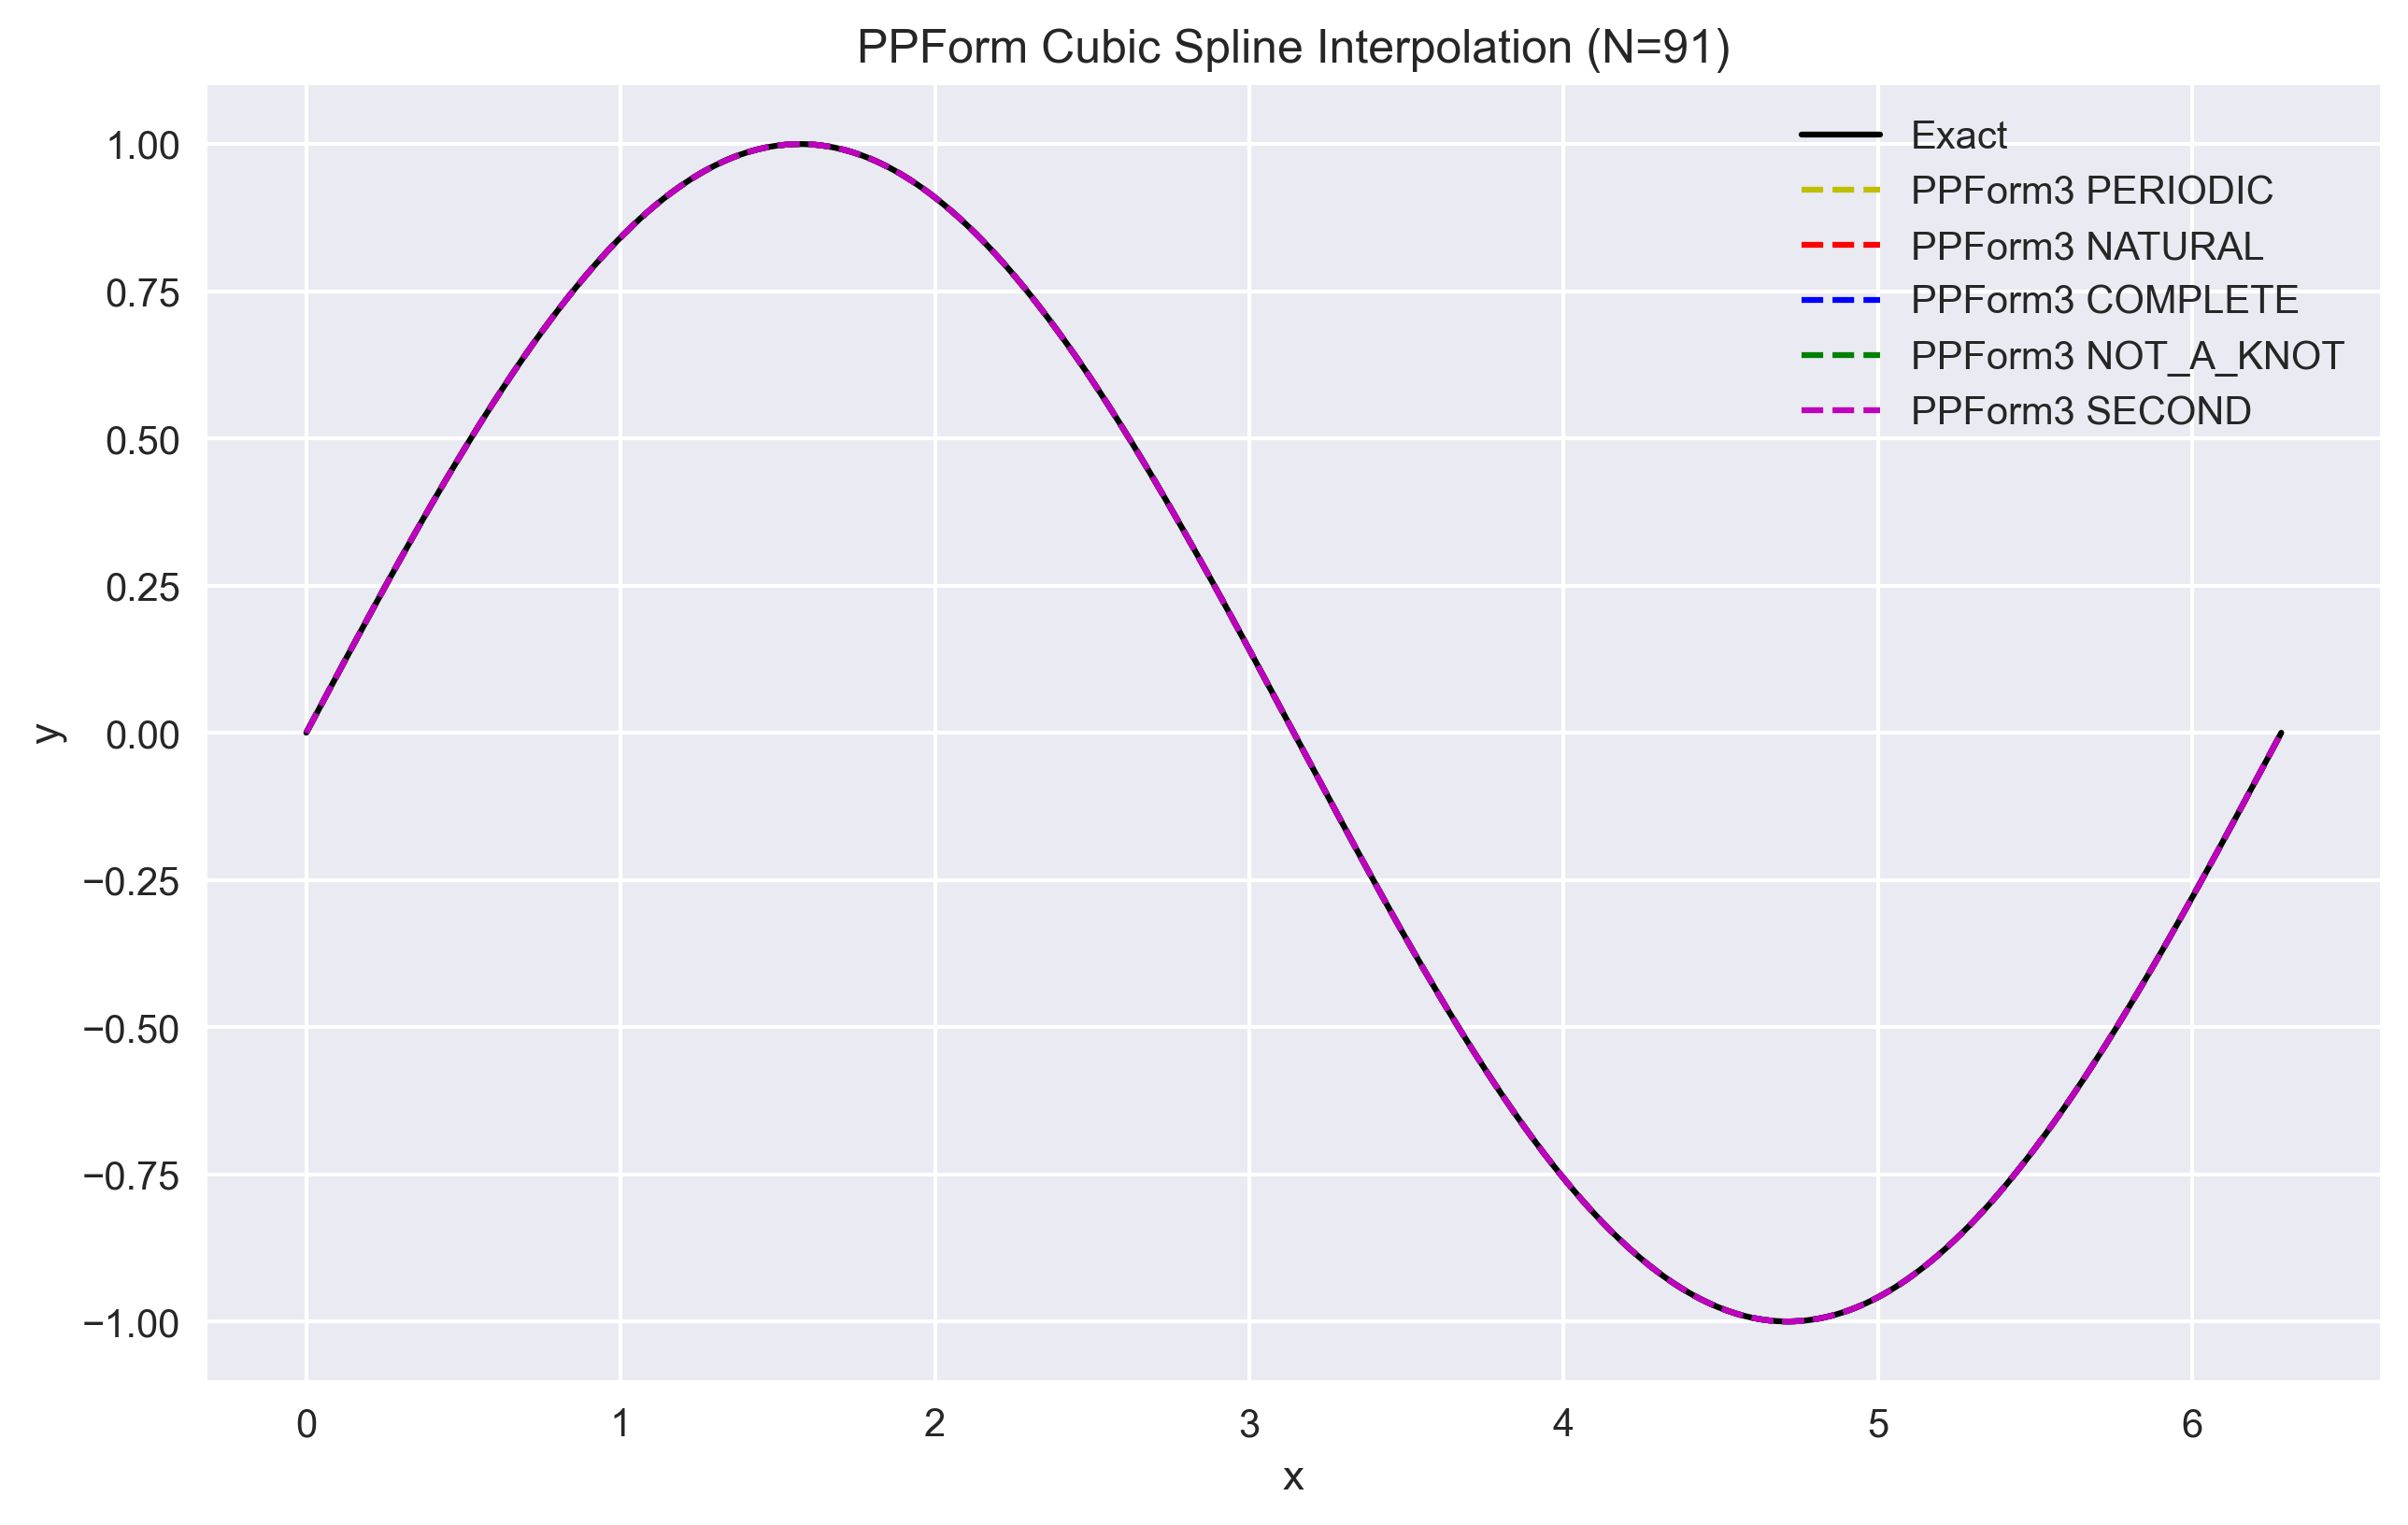
\includegraphics[width=0.45\textwidth]{../figure/test/PPForm3_N91.png} &
    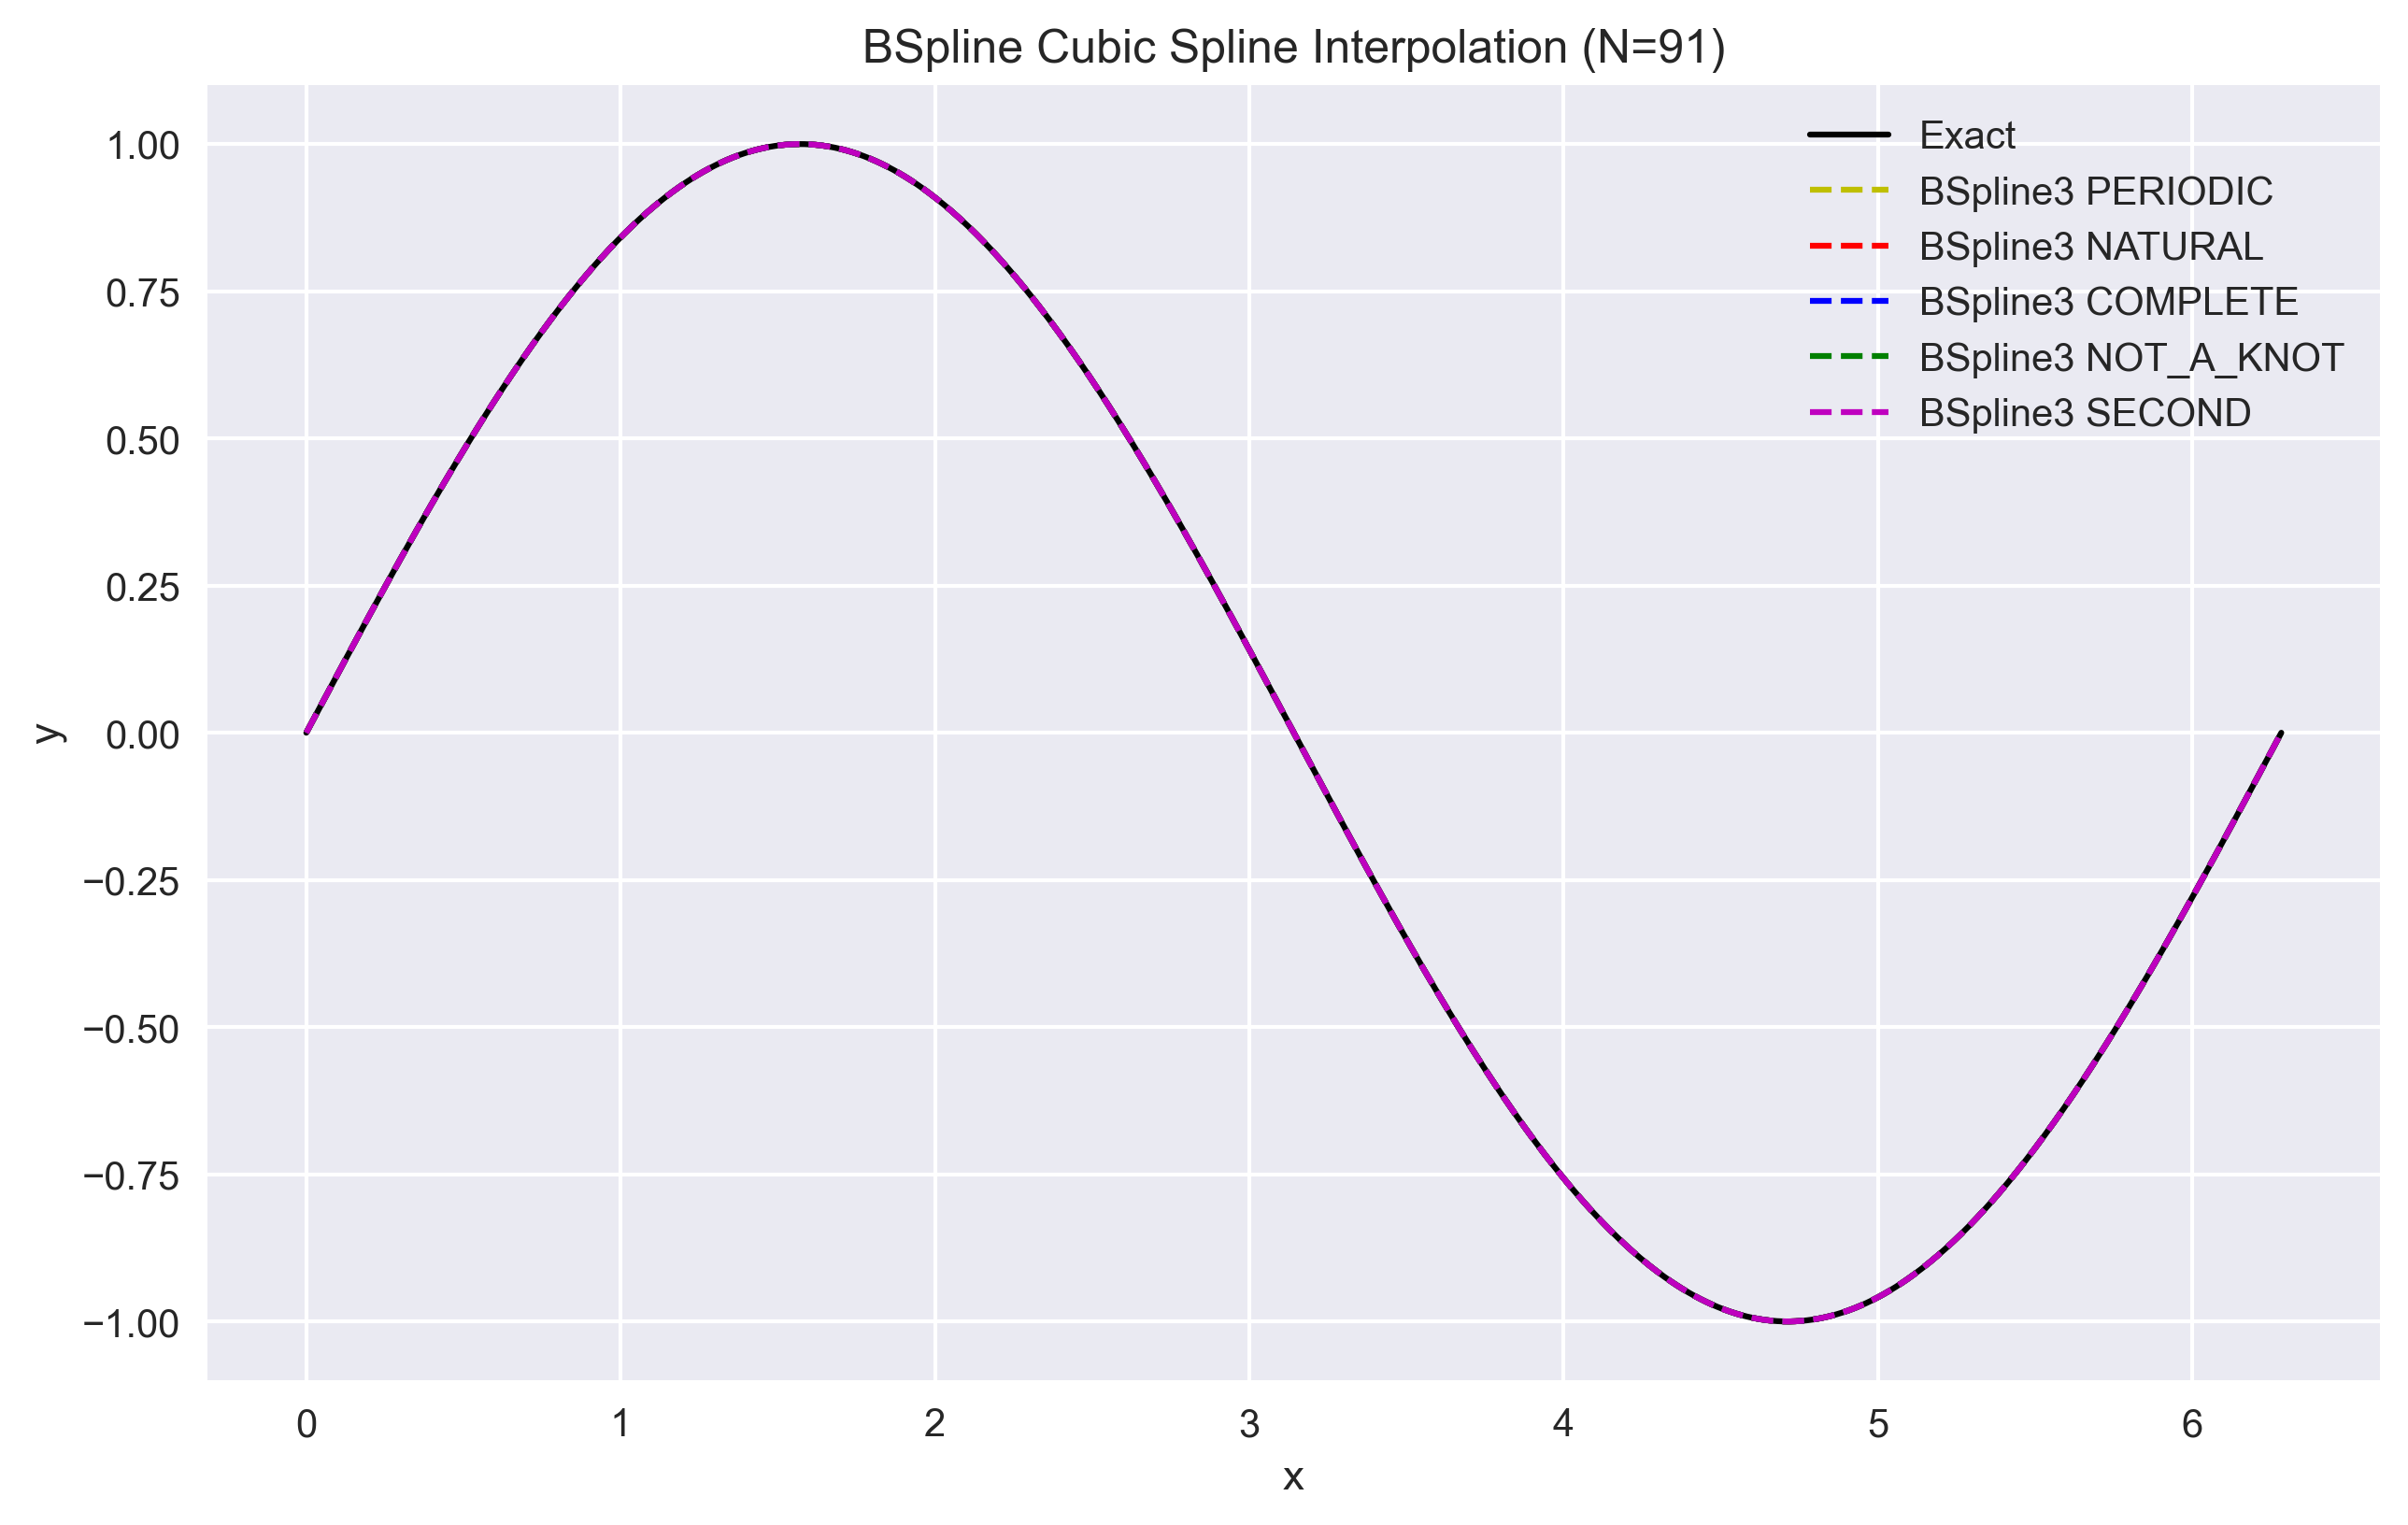
\includegraphics[width=0.45\textwidth]{../figure/test/BSpline3_N91.png}  \\
  \end{tabular}
  \renewcommand{\figurename}{Fig.}
  \caption{Comparison of quadratic PPForm and BSpline interpolation for different N values}
  \label{fig:test_quadratic}
\end{figure}

The error and convergence rate data for different methods and boundary conditions are shown in Table.\ref{tab:test_maxerror_convergence}:
It can be seen that under non-uniform node conditions, the fitting effect remains excellent, successfully achieving the fit.

\begin{table}[H]
  \centering
  \renewcommand{\tablename}{Table.}
  \caption{Max errors and convergence rates for different situations}
  \label{tab:test_maxerror_convergence}
  \pgfplotstabletypeset[
    col sep=comma,
    string type,
    columns/N/.style={
        column name=N,
        column type={|c}
      },
    columns/Method/.style={
        column name=Method,
        column type={|c}
      },
    columns/BoundaryCondition/.style={
        column name=BoundaryCondition,
        column type={|c},
        string replace*={_}{\_}
      },
    columns/MaxError/.style={
        column name=MaxError,
        column type={|c}
      },
    columns/ConvergenceRate/.style={
        column name=ConvergenceRate,
        column type={|c|} % Ensures the last column has a right border
      },
    every head row/.style={
        before row=\hline,
        after row=\hline
      },
    every last row/.style={
        after row=\hline
      },
  ]{../output/test/A_maxerror_convergence.csv}
\end{table}

\section{Intersection}
Compile and run the program \verb|intersect_test.cpp|. Its output includes the intersection information. The data stores in the directory \verb|output\intersect\intersect_curve.csv|.
Run the program \verb|plotIntersect.py| to plot the intersection curve $r_4$ with its self-intersection points calculated by python. The figures are stored in the directory \verb|figure/intersect|.

The program tests 4 curves including $r_1,r_2,r_3$ in problem E and a special curve $r_4$ for intersection. 
The formula for $r_4$ is 
$$
\begin{cases}
  x=\frac{3\sin t}{2}+a\sin\frac{3t}{2},\\
  y=\frac{3\cos t}{2}-a\cos\frac{3t}{2},
\end{cases}
$$
where $a$ is a constant. $a$ is 0.5 in the program and the interval is $[0,4\pi]$.

The figure of $r_4$ is shown in Fig.\ref{fig:r4_curve}.

\begin{figure}[H]
  \centering
  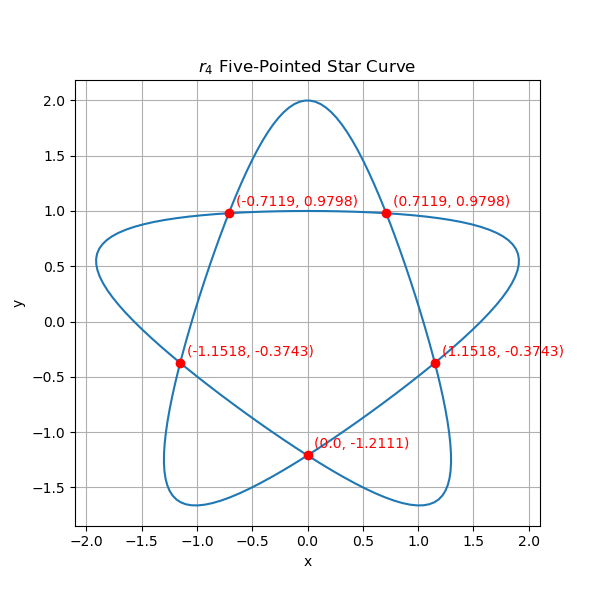
\includegraphics[width=0.6\textwidth]{../figure/intersect/five_pointed_star_curve.png}
  \renewcommand{\figurename}{Fig.}
  \caption{The figure of five pointed star curve \(r_4\)}
  \label{fig:r4_curve}
\end{figure}

The result is as follows:

\lstinputlisting{../output/intersect/intersect_curve.txt}

The results are consistent with the self-intersection conditions of the four curves. The calculation of the intersection points is also correct and within the computational error range.

\end{sloppypar}
\end{document}
